\documentclass{book}
\usepackage[a4paper,top=2.5cm,bottom=2.5cm,left=2.5cm,right=2.5cm]{geometry}
\usepackage{makeidx}
\usepackage{natbib}
\usepackage{graphicx}
\usepackage{multicol}
\usepackage{float}
\usepackage{listings}
\usepackage{color}
\usepackage{ifthen}
\usepackage[table]{xcolor}
\usepackage{textcomp}
\usepackage{alltt}
\usepackage[utf8]{inputenc}
\usepackage{mathptmx}
\usepackage[scaled=.90]{helvet}
\usepackage{courier}
\usepackage{sectsty}
\usepackage[titles]{tocloft}
\usepackage{doxygen}
\lstset{language=C++,inputencoding=utf8,basicstyle=\footnotesize,breaklines=true,breakatwhitespace=true,tabsize=5,numbers=left }
\makeindex
\setcounter{tocdepth}{3}
\renewcommand{\footrulewidth}{0.4pt}
\renewcommand{\familydefault}{\sfdefault}
\hfuzz=15pt
\setlength{\emergencystretch}{15pt}
\hbadness=750
\tolerance=750
\begin{document}
\begin{titlepage}
\vspace*{7cm}
\begin{center}
{\Large Phil\-Robokit }\\
\vspace*{1cm}
{\large Generated by Doxygen 1.8.1.1}\\
\vspace*{0.5cm}
{\small Sat Jul 14 2012 00:48:29}\\
\end{center}
\end{titlepage}
\clearemptydoublepage
\pagenumbering{roman}
\tableofcontents
\clearemptydoublepage
\pagenumbering{arabic}
\chapter{File Index}
\section{File List}
Here is a list of all files with brief descriptions\-:\begin{DoxyCompactList}
\item\contentsline{section}{{\bf Analog\-Output.\-phr} }{\pageref{_analog_output_8phr}}{}
\item\contentsline{section}{{\bf Blink\-Without\-Delay.\-phr} }{\pageref{_blink_without_delay_8phr}}{}
\item\contentsline{section}{{\bf corelib\-\_\-8bit\-\_\-timer.\-c} }{\pageref{corelib__8bit__timer_8c}}{}
\item\contentsline{section}{{\bf corelib\-\_\-8bit\-\_\-timer.\-h} }{\pageref{corelib__8bit__timer_8h}}{}
\item\contentsline{section}{{\bf corelib\-\_\-adc.\-c} }{\pageref{corelib__adc_8c}}{}
\item\contentsline{section}{{\bf corelib\-\_\-adc.\-h} }{\pageref{corelib__adc_8h}}{}
\item\contentsline{section}{{\bf corelib\-\_\-pwm.\-c} }{\pageref{corelib__pwm_8c}}{}
\item\contentsline{section}{{\bf corelib\-\_\-pwm.\-h} }{\pageref{corelib__pwm_8h}}{}
\item\contentsline{section}{{\bf corelib\-\_\-timer.\-c} }{\pageref{corelib__timer_8c}}{}
\item\contentsline{section}{{\bf corelib\-\_\-timer.\-h} }{\pageref{corelib__timer_8h}}{}
\item\contentsline{section}{{\bf corelib\-\_\-uart.\-c} }{\pageref{corelib__uart_8c}}{}
\item\contentsline{section}{{\bf corelib\-\_\-uart.\-h} }{\pageref{corelib__uart_8h}}{}
\item\contentsline{section}{{\bf corelib\-\_\-user\-\_\-interrupt.\-c} }{\pageref{corelib__user__interrupt_8c}}{}
\item\contentsline{section}{{\bf corelib\-\_\-user\-\_\-interrupt.\-h} }{\pageref{corelib__user__interrupt_8h}}{}
\item\contentsline{section}{{\bf htc\-\_\-16f87xa.\-h} }{\pageref{htc__16f87xa_8h}}{}
\item\contentsline{section}{{\bf htc\-\_\-16f87xa\-\_\-\-S\-P\-Lint.\-h} }{\pageref{htc__16f87xa___s_p_lint_8h}}{}
\item\contentsline{section}{{\bf htc\-\_\-common.\-h} }{\pageref{htc__common_8h}}{}
\item\contentsline{section}{{\bf htc\-\_\-common\-\_\-\-S\-P\-Lint.\-h} }{\pageref{htc__common___s_p_lint_8h}}{}
\item\contentsline{section}{{\bf i2c.\-c} }{\pageref{i2c_8c}}{}
\item\contentsline{section}{{\bf i2c.\-h} }{\pageref{i2c_8h}}{}
\item\contentsline{section}{{\bf Multiple\-Servos.\-phr} }{\pageref{_multiple_servos_8phr}}{}
\item\contentsline{section}{{\bf Phil\-Robo\-Kit\-\_\-\-Core\-Lib\-\_\-\-Data\-Types.\-h} }{\pageref{_phil_robo_kit___core_lib___data_types_8h}}{}
\item\contentsline{section}{{\bf Phil\-Robokit\-\_\-\-Core\-Lib\-\_\-\-Global\-Defs.\-c} }{\pageref{_phil_robokit___core_lib___global_defs_8c}}{}
\item\contentsline{section}{{\bf Phil\-Robo\-Kit\-\_\-\-Core\-Lib\-\_\-\-Header.\-h} }{\pageref{_phil_robo_kit___core_lib___header_8h}}{}
\item\contentsline{section}{{\bf Phil\-Robo\-Kit\-\_\-\-Core\-Lib\-\_\-\-Macro.\-c} }{\pageref{_phil_robo_kit___core_lib___macro_8c}}{}
\item\contentsline{section}{{\bf Phil\-Robo\-Kit\-\_\-\-Core\-Lib\-\_\-\-Macro.\-h} }{\pageref{_phil_robo_kit___core_lib___macro_8h}}{}
\item\contentsline{section}{{\bf P\-P\-M\-Generator.\-phr} }{\pageref{_p_p_m_generator_8phr}}{}
\item\contentsline{section}{{\bf P\-W\-M.\-phr} }{\pageref{_p_w_m_8phr}}{}
\item\contentsline{section}{{\bf servo.\-c} }{\pageref{servo_8c}}{}
\item\contentsline{section}{{\bf servo.\-h} }{\pageref{servo_8h}}{}
\item\contentsline{section}{{\bf Servo\-Port.\-phr} }{\pageref{_servo_port_8phr}}{}
\item\contentsline{section}{{\bf Servos.\-phr} }{\pageref{_servos_8phr}}{}
\item\contentsline{section}{{\bf spi.\-c} }{\pageref{spi_8c}}{}
\item\contentsline{section}{{\bf spi.\-h} }{\pageref{spi_8h}}{}
\item\contentsline{section}{{\bf User\-Interrupt.\-phr} }{\pageref{_user_interrupt_8phr}}{}
\end{DoxyCompactList}

\chapter{File Documentation}
\section{Analog\-Output.\-phr File Reference}
\label{_analog_output_8phr}\index{Analog\-Output.\-phr@{Analog\-Output.\-phr}}
\subsection*{Functions}
\begin{DoxyCompactItemize}
\item 
void {\bf init} ()
\item 
void {\bf program} ()
\end{DoxyCompactItemize}


\subsection{Function Documentation}
\index{Analog\-Output.\-phr@{Analog\-Output.\-phr}!init@{init}}
\index{init@{init}!AnalogOutput.phr@{Analog\-Output.\-phr}}
\subsubsection[{init}]{\setlength{\rightskip}{0pt plus 5cm}void init (
\begin{DoxyParamCaption}
\item[{void}]{}
\end{DoxyParamCaption}
)}\label{_analog_output_8phr_a02fd73d861ef2e4aabb38c0c9ff82947}


Definition at line 6 of file Analog\-Output.\-phr.



Here is the call graph for this function\-:\nopagebreak
\begin{figure}[H]
\begin{center}
\leavevmode
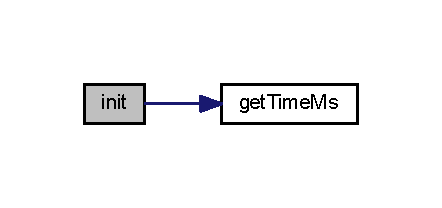
\includegraphics[width=212pt]{_analog_output_8phr_a02fd73d861ef2e4aabb38c0c9ff82947_cgraph}
\end{center}
\end{figure}


\index{Analog\-Output.\-phr@{Analog\-Output.\-phr}!program@{program}}
\index{program@{program}!AnalogOutput.phr@{Analog\-Output.\-phr}}
\subsubsection[{program}]{\setlength{\rightskip}{0pt plus 5cm}void program (
\begin{DoxyParamCaption}
\item[{void}]{}
\end{DoxyParamCaption}
)}\label{_analog_output_8phr_aaed33fe77209e582d96078370b5f8da4}


Definition at line 11 of file Analog\-Output.\-phr.



Here is the call graph for this function\-:\nopagebreak
\begin{figure}[H]
\begin{center}
\leavevmode
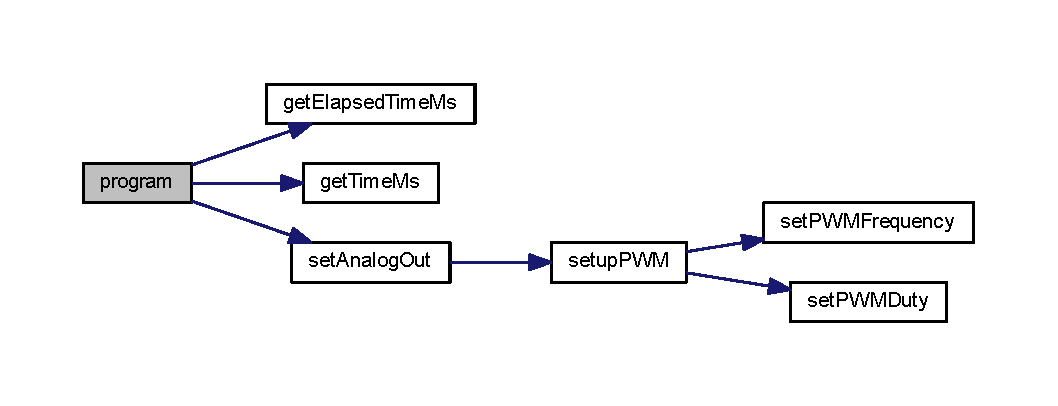
\includegraphics[width=350pt]{_analog_output_8phr_aaed33fe77209e582d96078370b5f8da4_cgraph}
\end{center}
\end{figure}



\section{Blink\-Without\-Delay.\-phr File Reference}
\label{_blink_without_delay_8phr}\index{Blink\-Without\-Delay.\-phr@{Blink\-Without\-Delay.\-phr}}
\subsection*{Functions}
\begin{DoxyCompactItemize}
\item 
void {\bf init} ()
\item 
void {\bf program} ()
\end{DoxyCompactItemize}
\subsection*{Variables}
\begin{DoxyCompactItemize}
\item 
unsigned int {\bf Timer}
\end{DoxyCompactItemize}


\subsection{Function Documentation}
\index{Blink\-Without\-Delay.\-phr@{Blink\-Without\-Delay.\-phr}!init@{init}}
\index{init@{init}!BlinkWithoutDelay.phr@{Blink\-Without\-Delay.\-phr}}
\subsubsection[{init}]{\setlength{\rightskip}{0pt plus 5cm}void init (
\begin{DoxyParamCaption}
\item[{void}]{}
\end{DoxyParamCaption}
)}\label{_blink_without_delay_8phr_a02fd73d861ef2e4aabb38c0c9ff82947}


Definition at line 17 of file Blink\-Without\-Delay.\-phr.



Here is the call graph for this function\-:\nopagebreak
\begin{figure}[H]
\begin{center}
\leavevmode
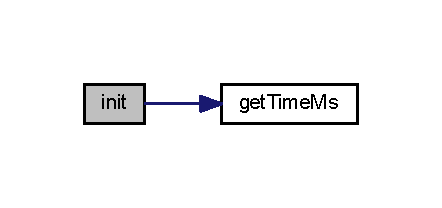
\includegraphics[width=212pt]{_blink_without_delay_8phr_a02fd73d861ef2e4aabb38c0c9ff82947_cgraph}
\end{center}
\end{figure}


\index{Blink\-Without\-Delay.\-phr@{Blink\-Without\-Delay.\-phr}!program@{program}}
\index{program@{program}!BlinkWithoutDelay.phr@{Blink\-Without\-Delay.\-phr}}
\subsubsection[{program}]{\setlength{\rightskip}{0pt plus 5cm}void program (
\begin{DoxyParamCaption}
\item[{void}]{}
\end{DoxyParamCaption}
)}\label{_blink_without_delay_8phr_aaed33fe77209e582d96078370b5f8da4}


Definition at line 27 of file Blink\-Without\-Delay.\-phr.



Here is the call graph for this function\-:\nopagebreak
\begin{figure}[H]
\begin{center}
\leavevmode
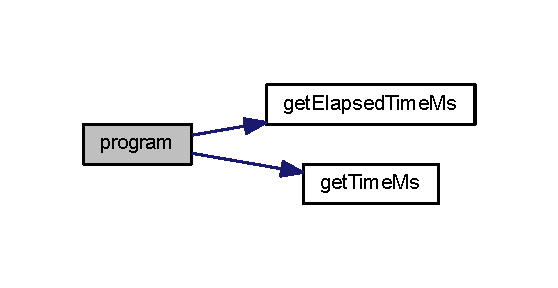
\includegraphics[width=268pt]{_blink_without_delay_8phr_aaed33fe77209e582d96078370b5f8da4_cgraph}
\end{center}
\end{figure}




\subsection{Variable Documentation}
\index{Blink\-Without\-Delay.\-phr@{Blink\-Without\-Delay.\-phr}!Timer@{Timer}}
\index{Timer@{Timer}!BlinkWithoutDelay.phr@{Blink\-Without\-Delay.\-phr}}
\subsubsection[{Timer}]{\setlength{\rightskip}{0pt plus 5cm}unsigned int Timer}\label{_blink_without_delay_8phr_a4ca5eb0caf1598b631642d7ef56bfa21}


Definition at line 13 of file Blink\-Without\-Delay.\-phr.


\section{corelib\-\_\-8bit\-\_\-timer.\-c File Reference}
\label{corelib__8bit__timer_8c}\index{corelib\-\_\-8bit\-\_\-timer.\-c@{corelib\-\_\-8bit\-\_\-timer.\-c}}
{\ttfamily \#include \char`\"{}corelib\-\_\-8bit\-\_\-timer.\-h\char`\"{}}\\*
Include dependency graph for corelib\-\_\-8bit\-\_\-timer.\-c\-:\nopagebreak
\begin{figure}[H]
\begin{center}
\leavevmode
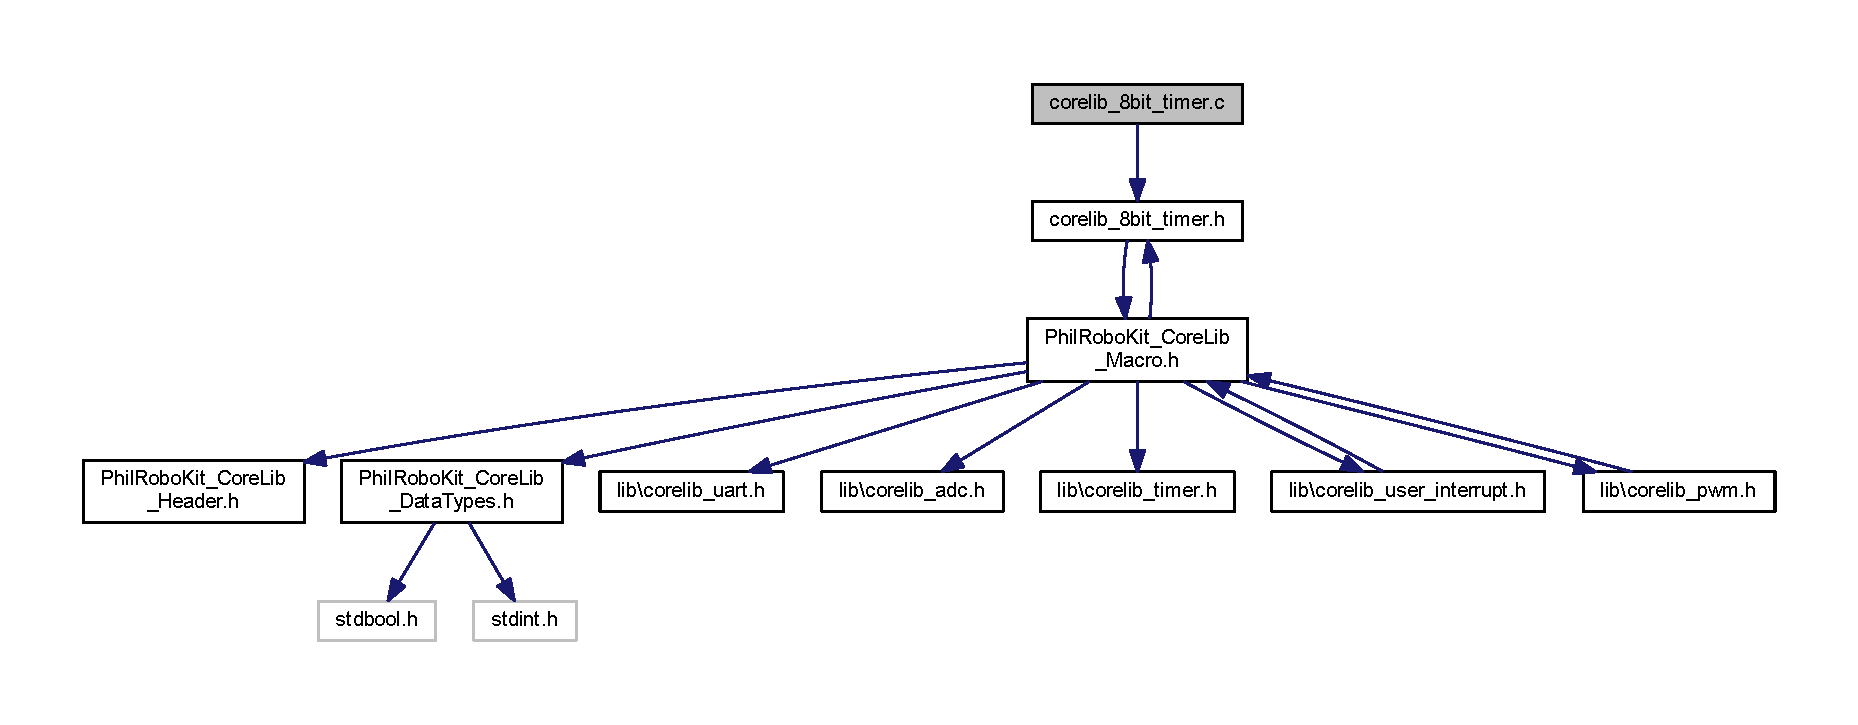
\includegraphics[width=350pt]{corelib__8bit__timer_8c__incl}
\end{center}
\end{figure}
\subsection*{Functions}
\begin{DoxyCompactItemize}
\item 
void {\bf setup8\-Bit\-Timer\-Def} (enum {\bf e\-Tmr\-Modules} tmr\-Module, void($\ast$function)())
\item 
void {\bf setup8\-Bit\-Timer} (enum {\bf e\-Tmr\-Modules} tmr\-Module, uint8\-\_\-t ui8\-Prescaler, uint8\-\_\-t ui8\-Postscaler)
\item 
void {\bf set\-Timer\-Value} (enum {\bf e\-Tmr\-Modules} tmr\-Module, uint8\-\_\-t ui8\-Value)
\item 
void {\bf timer8bit\-Interrupt\-Handler} (void)
\end{DoxyCompactItemize}
\subsection*{Variables}
\begin{DoxyCompactItemize}
\item 
void($\ast$ {\bf pt2\-T\-M\-R2} )() = \&null\-T\-M\-R\-Function
\end{DoxyCompactItemize}


\subsection{Function Documentation}
\index{corelib\-\_\-8bit\-\_\-timer.\-c@{corelib\-\_\-8bit\-\_\-timer.\-c}!set\-Timer\-Value@{set\-Timer\-Value}}
\index{set\-Timer\-Value@{set\-Timer\-Value}!corelib_8bit_timer.c@{corelib\-\_\-8bit\-\_\-timer.\-c}}
\subsubsection[{set\-Timer\-Value}]{\setlength{\rightskip}{0pt plus 5cm}void set\-Timer\-Value (
\begin{DoxyParamCaption}
\item[{enum {\bf e\-Tmr\-Modules}}]{tmr\-Module, }
\item[{uint8\-\_\-t}]{ui8\-Value}
\end{DoxyParamCaption}
)}\label{corelib__8bit__timer_8c_a2d25345b7b4cad4443ad55dd860f9bdf}


Definition at line 129 of file corelib\-\_\-8bit\-\_\-timer.\-c.

\index{corelib\-\_\-8bit\-\_\-timer.\-c@{corelib\-\_\-8bit\-\_\-timer.\-c}!setup8\-Bit\-Timer@{setup8\-Bit\-Timer}}
\index{setup8\-Bit\-Timer@{setup8\-Bit\-Timer}!corelib_8bit_timer.c@{corelib\-\_\-8bit\-\_\-timer.\-c}}
\subsubsection[{setup8\-Bit\-Timer}]{\setlength{\rightskip}{0pt plus 5cm}void setup8\-Bit\-Timer (
\begin{DoxyParamCaption}
\item[{enum {\bf e\-Tmr\-Modules}}]{tmr\-Module, }
\item[{uint8\-\_\-t}]{ui8\-Prescaler, }
\item[{uint8\-\_\-t}]{ui8\-Postscaler}
\end{DoxyParamCaption}
)}\label{corelib__8bit__timer_8c_a2b810b302fcd351ee1c1638af675fe88}


Definition at line 101 of file corelib\-\_\-8bit\-\_\-timer.\-c.

\index{corelib\-\_\-8bit\-\_\-timer.\-c@{corelib\-\_\-8bit\-\_\-timer.\-c}!setup8\-Bit\-Timer\-Def@{setup8\-Bit\-Timer\-Def}}
\index{setup8\-Bit\-Timer\-Def@{setup8\-Bit\-Timer\-Def}!corelib_8bit_timer.c@{corelib\-\_\-8bit\-\_\-timer.\-c}}
\subsubsection[{setup8\-Bit\-Timer\-Def}]{\setlength{\rightskip}{0pt plus 5cm}void setup8\-Bit\-Timer\-Def (
\begin{DoxyParamCaption}
\item[{enum {\bf e\-Tmr\-Modules}}]{tmr\-Module, }
\item[{void($\ast$)()}]{function}
\end{DoxyParamCaption}
)}\label{corelib__8bit__timer_8c_ad5862ac054692c86c9061c7f41ac6239}


Definition at line 70 of file corelib\-\_\-8bit\-\_\-timer.\-c.

\index{corelib\-\_\-8bit\-\_\-timer.\-c@{corelib\-\_\-8bit\-\_\-timer.\-c}!timer8bit\-Interrupt\-Handler@{timer8bit\-Interrupt\-Handler}}
\index{timer8bit\-Interrupt\-Handler@{timer8bit\-Interrupt\-Handler}!corelib_8bit_timer.c@{corelib\-\_\-8bit\-\_\-timer.\-c}}
\subsubsection[{timer8bit\-Interrupt\-Handler}]{\setlength{\rightskip}{0pt plus 5cm}void timer8bit\-Interrupt\-Handler (
\begin{DoxyParamCaption}
\item[{void}]{}
\end{DoxyParamCaption}
)}\label{corelib__8bit__timer_8c_ae50d8b3d1589fa043eb15e8644275f1b}


Definition at line 165 of file corelib\-\_\-8bit\-\_\-timer.\-c.



\subsection{Variable Documentation}
\index{corelib\-\_\-8bit\-\_\-timer.\-c@{corelib\-\_\-8bit\-\_\-timer.\-c}!pt2\-T\-M\-R2@{pt2\-T\-M\-R2}}
\index{pt2\-T\-M\-R2@{pt2\-T\-M\-R2}!corelib_8bit_timer.c@{corelib\-\_\-8bit\-\_\-timer.\-c}}
\subsubsection[{pt2\-T\-M\-R2}]{\setlength{\rightskip}{0pt plus 5cm}void($\ast$ pt2\-T\-M\-R2)() = \&null\-T\-M\-R\-Function}\label{corelib__8bit__timer_8c_a0068139de556494b576b4715d623e719}


Definition at line 40 of file corelib\-\_\-8bit\-\_\-timer.\-c.


\section{corelib\-\_\-8bit\-\_\-timer.\-h File Reference}
\label{corelib__8bit__timer_8h}\index{corelib\-\_\-8bit\-\_\-timer.\-h@{corelib\-\_\-8bit\-\_\-timer.\-h}}
{\ttfamily \#include $<$Phil\-Robo\-Kit\-\_\-\-Core\-Lib\-\_\-\-Macro.\-h$>$}\\*
Include dependency graph for corelib\-\_\-8bit\-\_\-timer.\-h\-:\nopagebreak
\begin{figure}[H]
\begin{center}
\leavevmode
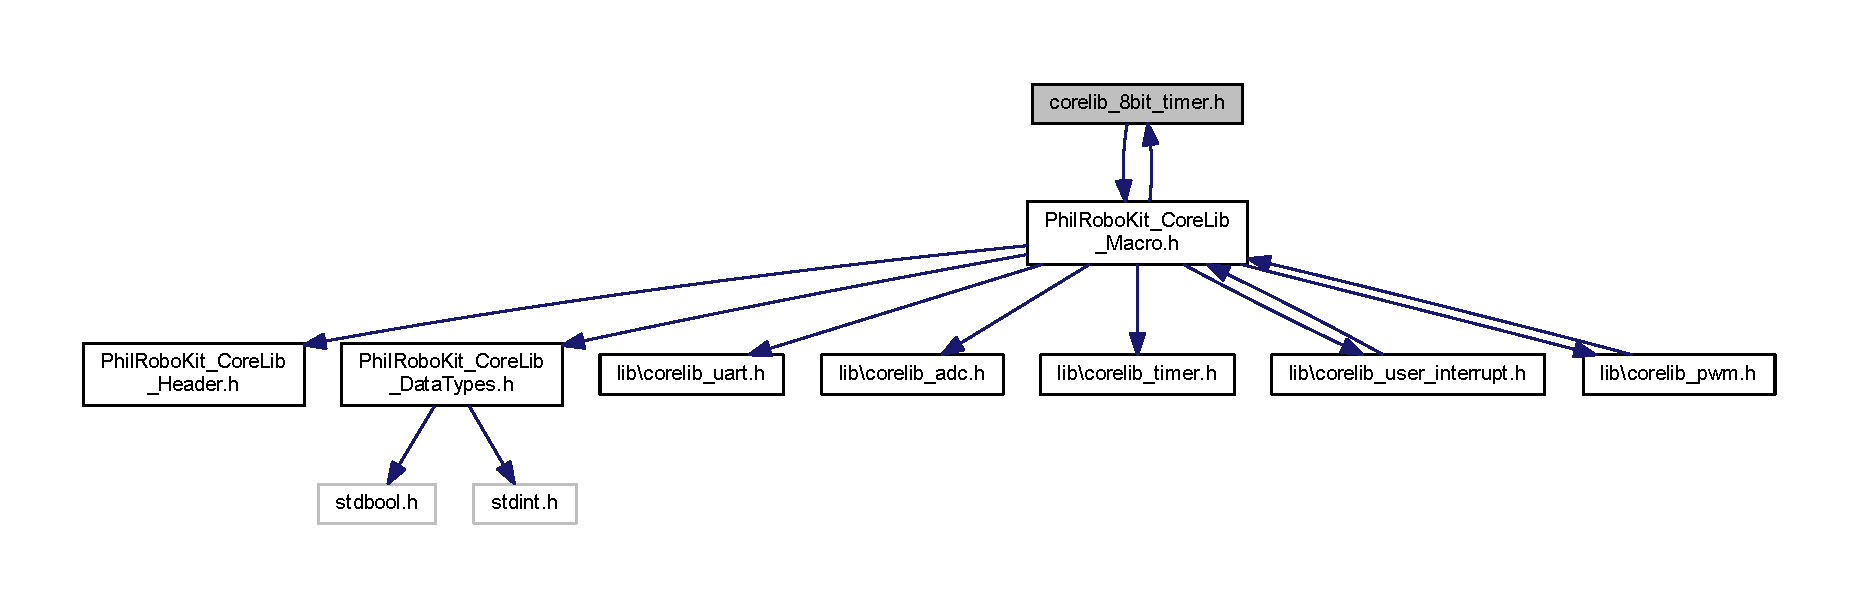
\includegraphics[width=350pt]{corelib__8bit__timer_8h__incl}
\end{center}
\end{figure}
This graph shows which files directly or indirectly include this file\-:\nopagebreak
\begin{figure}[H]
\begin{center}
\leavevmode
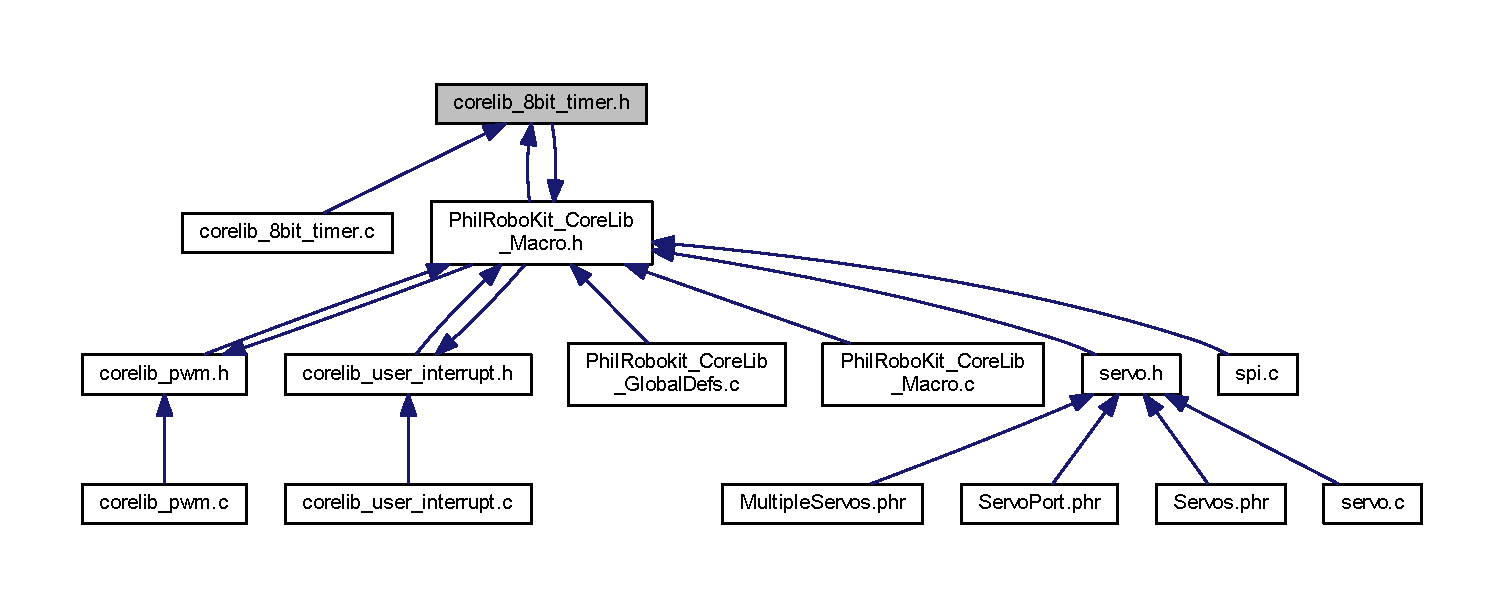
\includegraphics[width=350pt]{corelib__8bit__timer_8h__dep__incl}
\end{center}
\end{figure}
\subsection*{Macros}
\begin{DoxyCompactItemize}
\item 
\#define {\bf T\-I\-M\-E\-R\-\_\-8\-B\-I\-T\-\_\-\-E\-N\-A\-B\-L\-E\-D}~{\bf T\-R\-U\-E}
\item 
\#define {\bf T\-I\-M\-E\-R2\-\_\-\-E\-N\-A\-B\-L\-E\-D}~{\bf T\-R\-U\-E}
\item 
\#define {\bf mc\-\_\-timer2\-Int\-En}()~({\bf B\-I\-T\-\_\-\-P\-I\-E1\-\_\-\-T\-M\-R2\-I\-E} = 1)
\item 
\#define {\bf mc\-\_\-timer2\-Int\-Dis}()~({\bf B\-I\-T\-\_\-\-P\-I\-E1\-\_\-\-T\-M\-R2\-I\-E} = 0)
\item 
\#define {\bf mc\-\_\-timer2\-I\-F\-Clr}()~({\bf B\-I\-T\-\_\-\-P\-I\-R1\-\_\-\-T\-M\-R2\-I\-F} = 0)
\item 
\#define {\bf mc\-\_\-enable\-T\-M\-R2}()~({\bf B\-I\-T\-\_\-\-T2\-C\-O\-N\-\_\-\-T\-M\-R2\-O\-N} = 1)
\item 
\#define {\bf mc\-\_\-disable\-T\-M\-R2}()~({\bf B\-I\-T\-\_\-\-T2\-C\-O\-N\-\_\-\-T\-M\-R2\-O\-N} = 0)
\item 
\#define {\bf mc\-\_\-clear\-T\-M\-R2\-I\-F}()
\item 
\#define {\bf mc\-\_\-set\-T\-M\-R2\-Prescaler}(a)
\item 
\#define {\bf mc\-\_\-set\-T\-M\-R2\-Postscaler}(a)
\end{DoxyCompactItemize}
\subsection*{Enumerations}
\begin{DoxyCompactItemize}
\item 
enum {\bf e\-Tmr\-Modules} \{ {\bf T\-I\-M\-E\-R2} =  2, 
{\bf T\-I\-M\-E\-R4} =  4, 
{\bf T\-I\-M\-E\-R6} =  6
 \}
\end{DoxyCompactItemize}
\subsection*{Functions}
\begin{DoxyCompactItemize}
\item 
void {\bf timer8bit\-Interrupt\-Handler} (void)
\item 
void {\bf setup8\-Bit\-Timer\-Def} (enum {\bf e\-Tmr\-Modules} tmr\-Module, void($\ast$function)())
\item 
void {\bf setup8\-Bit\-Timer} (enum {\bf e\-Tmr\-Modules} tmr\-Module, uint8\-\_\-t ui8\-Prescaler, uint8\-\_\-t ui8\-Postscaler)
\item 
void {\bf set\-Timer\-Value} (enum {\bf e\-Tmr\-Modules} tmr\-Module, uint8\-\_\-t ui8\-Value)
\end{DoxyCompactItemize}


\subsection{Macro Definition Documentation}
\index{corelib\-\_\-8bit\-\_\-timer.\-h@{corelib\-\_\-8bit\-\_\-timer.\-h}!mc\-\_\-clear\-T\-M\-R2\-I\-F@{mc\-\_\-clear\-T\-M\-R2\-I\-F}}
\index{mc\-\_\-clear\-T\-M\-R2\-I\-F@{mc\-\_\-clear\-T\-M\-R2\-I\-F}!corelib_8bit_timer.h@{corelib\-\_\-8bit\-\_\-timer.\-h}}
\subsubsection[{mc\-\_\-clear\-T\-M\-R2\-I\-F}]{\setlength{\rightskip}{0pt plus 5cm}\#define mc\-\_\-clear\-T\-M\-R2\-I\-F(
\begin{DoxyParamCaption}
{}
\end{DoxyParamCaption}
)}\label{corelib__8bit__timer_8h_a68c7aa77163ea49bef2298213ffcc5b3}


Definition at line 74 of file corelib\-\_\-8bit\-\_\-timer.\-h.

\index{corelib\-\_\-8bit\-\_\-timer.\-h@{corelib\-\_\-8bit\-\_\-timer.\-h}!mc\-\_\-disable\-T\-M\-R2@{mc\-\_\-disable\-T\-M\-R2}}
\index{mc\-\_\-disable\-T\-M\-R2@{mc\-\_\-disable\-T\-M\-R2}!corelib_8bit_timer.h@{corelib\-\_\-8bit\-\_\-timer.\-h}}
\subsubsection[{mc\-\_\-disable\-T\-M\-R2}]{\setlength{\rightskip}{0pt plus 5cm}\#define mc\-\_\-disable\-T\-M\-R2(
\begin{DoxyParamCaption}
{}
\end{DoxyParamCaption}
)~({\bf B\-I\-T\-\_\-\-T2\-C\-O\-N\-\_\-\-T\-M\-R2\-O\-N} = 0)}\label{corelib__8bit__timer_8h_aee737045d808621d63fdf2abefc0b11b}


Definition at line 72 of file corelib\-\_\-8bit\-\_\-timer.\-h.

\index{corelib\-\_\-8bit\-\_\-timer.\-h@{corelib\-\_\-8bit\-\_\-timer.\-h}!mc\-\_\-enable\-T\-M\-R2@{mc\-\_\-enable\-T\-M\-R2}}
\index{mc\-\_\-enable\-T\-M\-R2@{mc\-\_\-enable\-T\-M\-R2}!corelib_8bit_timer.h@{corelib\-\_\-8bit\-\_\-timer.\-h}}
\subsubsection[{mc\-\_\-enable\-T\-M\-R2}]{\setlength{\rightskip}{0pt plus 5cm}\#define mc\-\_\-enable\-T\-M\-R2(
\begin{DoxyParamCaption}
{}
\end{DoxyParamCaption}
)~({\bf B\-I\-T\-\_\-\-T2\-C\-O\-N\-\_\-\-T\-M\-R2\-O\-N} = 1)}\label{corelib__8bit__timer_8h_a1ee851a06b82d6c8b8244cf30da540ba}


Definition at line 70 of file corelib\-\_\-8bit\-\_\-timer.\-h.

\index{corelib\-\_\-8bit\-\_\-timer.\-h@{corelib\-\_\-8bit\-\_\-timer.\-h}!mc\-\_\-set\-T\-M\-R2\-Postscaler@{mc\-\_\-set\-T\-M\-R2\-Postscaler}}
\index{mc\-\_\-set\-T\-M\-R2\-Postscaler@{mc\-\_\-set\-T\-M\-R2\-Postscaler}!corelib_8bit_timer.h@{corelib\-\_\-8bit\-\_\-timer.\-h}}
\subsubsection[{mc\-\_\-set\-T\-M\-R2\-Postscaler}]{\setlength{\rightskip}{0pt plus 5cm}\#define mc\-\_\-set\-T\-M\-R2\-Postscaler(
\begin{DoxyParamCaption}
\item[{}]{a}
\end{DoxyParamCaption}
)}\label{corelib__8bit__timer_8h_adf0aead416561df0501816fc76e1b745}
{\bfseries Value\-:}
\begin{DoxyCode}
REGISTER_T2CON &=~TMR_POSTSCALE_MASK;             \(\backslash\)
     REGISTER\_T2CON |= (a<<3)&TMR_POSTSCALE_MASK
\end{DoxyCode}


Definition at line 82 of file corelib\-\_\-8bit\-\_\-timer.\-h.

\index{corelib\-\_\-8bit\-\_\-timer.\-h@{corelib\-\_\-8bit\-\_\-timer.\-h}!mc\-\_\-set\-T\-M\-R2\-Prescaler@{mc\-\_\-set\-T\-M\-R2\-Prescaler}}
\index{mc\-\_\-set\-T\-M\-R2\-Prescaler@{mc\-\_\-set\-T\-M\-R2\-Prescaler}!corelib_8bit_timer.h@{corelib\-\_\-8bit\-\_\-timer.\-h}}
\subsubsection[{mc\-\_\-set\-T\-M\-R2\-Prescaler}]{\setlength{\rightskip}{0pt plus 5cm}\#define mc\-\_\-set\-T\-M\-R2\-Prescaler(
\begin{DoxyParamCaption}
\item[{}]{a}
\end{DoxyParamCaption}
)}\label{corelib__8bit__timer_8h_a460e04b9afdf2393e36f572174e3ca10}
{\bfseries Value\-:}
\begin{DoxyCode}
REGISTER_T2CON &=~TMR_PRESCALE_MASK;              \(\backslash\)
     REGISTER\_T2CON |= a&TMR_PRESCALE_MASK
\end{DoxyCode}


Definition at line 77 of file corelib\-\_\-8bit\-\_\-timer.\-h.

\index{corelib\-\_\-8bit\-\_\-timer.\-h@{corelib\-\_\-8bit\-\_\-timer.\-h}!mc\-\_\-timer2\-I\-F\-Clr@{mc\-\_\-timer2\-I\-F\-Clr}}
\index{mc\-\_\-timer2\-I\-F\-Clr@{mc\-\_\-timer2\-I\-F\-Clr}!corelib_8bit_timer.h@{corelib\-\_\-8bit\-\_\-timer.\-h}}
\subsubsection[{mc\-\_\-timer2\-I\-F\-Clr}]{\setlength{\rightskip}{0pt plus 5cm}\#define mc\-\_\-timer2\-I\-F\-Clr(
\begin{DoxyParamCaption}
{}
\end{DoxyParamCaption}
)~({\bf B\-I\-T\-\_\-\-P\-I\-R1\-\_\-\-T\-M\-R2\-I\-F} = 0)}\label{corelib__8bit__timer_8h_a5b8e6f6b267dc9ed3db177ce593d717a}


Definition at line 67 of file corelib\-\_\-8bit\-\_\-timer.\-h.

\index{corelib\-\_\-8bit\-\_\-timer.\-h@{corelib\-\_\-8bit\-\_\-timer.\-h}!mc\-\_\-timer2\-Int\-Dis@{mc\-\_\-timer2\-Int\-Dis}}
\index{mc\-\_\-timer2\-Int\-Dis@{mc\-\_\-timer2\-Int\-Dis}!corelib_8bit_timer.h@{corelib\-\_\-8bit\-\_\-timer.\-h}}
\subsubsection[{mc\-\_\-timer2\-Int\-Dis}]{\setlength{\rightskip}{0pt plus 5cm}\#define mc\-\_\-timer2\-Int\-Dis(
\begin{DoxyParamCaption}
{}
\end{DoxyParamCaption}
)~({\bf B\-I\-T\-\_\-\-P\-I\-E1\-\_\-\-T\-M\-R2\-I\-E} = 0)}\label{corelib__8bit__timer_8h_a96de9ffd78071d0096ad16aedaa965bc}


Definition at line 65 of file corelib\-\_\-8bit\-\_\-timer.\-h.

\index{corelib\-\_\-8bit\-\_\-timer.\-h@{corelib\-\_\-8bit\-\_\-timer.\-h}!mc\-\_\-timer2\-Int\-En@{mc\-\_\-timer2\-Int\-En}}
\index{mc\-\_\-timer2\-Int\-En@{mc\-\_\-timer2\-Int\-En}!corelib_8bit_timer.h@{corelib\-\_\-8bit\-\_\-timer.\-h}}
\subsubsection[{mc\-\_\-timer2\-Int\-En}]{\setlength{\rightskip}{0pt plus 5cm}\#define mc\-\_\-timer2\-Int\-En(
\begin{DoxyParamCaption}
{}
\end{DoxyParamCaption}
)~({\bf B\-I\-T\-\_\-\-P\-I\-E1\-\_\-\-T\-M\-R2\-I\-E} = 1)}\label{corelib__8bit__timer_8h_a418288f933a390f6c8a7ca4d531946c6}


Definition at line 63 of file corelib\-\_\-8bit\-\_\-timer.\-h.

\index{corelib\-\_\-8bit\-\_\-timer.\-h@{corelib\-\_\-8bit\-\_\-timer.\-h}!T\-I\-M\-E\-R2\-\_\-\-E\-N\-A\-B\-L\-E\-D@{T\-I\-M\-E\-R2\-\_\-\-E\-N\-A\-B\-L\-E\-D}}
\index{T\-I\-M\-E\-R2\-\_\-\-E\-N\-A\-B\-L\-E\-D@{T\-I\-M\-E\-R2\-\_\-\-E\-N\-A\-B\-L\-E\-D}!corelib_8bit_timer.h@{corelib\-\_\-8bit\-\_\-timer.\-h}}
\subsubsection[{T\-I\-M\-E\-R2\-\_\-\-E\-N\-A\-B\-L\-E\-D}]{\setlength{\rightskip}{0pt plus 5cm}\#define T\-I\-M\-E\-R2\-\_\-\-E\-N\-A\-B\-L\-E\-D~{\bf T\-R\-U\-E}}\label{corelib__8bit__timer_8h_a83440b416ee46c2066df4336d3996716}


Definition at line 56 of file corelib\-\_\-8bit\-\_\-timer.\-h.

\index{corelib\-\_\-8bit\-\_\-timer.\-h@{corelib\-\_\-8bit\-\_\-timer.\-h}!T\-I\-M\-E\-R\-\_\-8\-B\-I\-T\-\_\-\-E\-N\-A\-B\-L\-E\-D@{T\-I\-M\-E\-R\-\_\-8\-B\-I\-T\-\_\-\-E\-N\-A\-B\-L\-E\-D}}
\index{T\-I\-M\-E\-R\-\_\-8\-B\-I\-T\-\_\-\-E\-N\-A\-B\-L\-E\-D@{T\-I\-M\-E\-R\-\_\-8\-B\-I\-T\-\_\-\-E\-N\-A\-B\-L\-E\-D}!corelib_8bit_timer.h@{corelib\-\_\-8bit\-\_\-timer.\-h}}
\subsubsection[{T\-I\-M\-E\-R\-\_\-8\-B\-I\-T\-\_\-\-E\-N\-A\-B\-L\-E\-D}]{\setlength{\rightskip}{0pt plus 5cm}\#define T\-I\-M\-E\-R\-\_\-8\-B\-I\-T\-\_\-\-E\-N\-A\-B\-L\-E\-D~{\bf T\-R\-U\-E}}\label{corelib__8bit__timer_8h_aa1cb2ea285c3d3f67955a24966e82f42}


Definition at line 55 of file corelib\-\_\-8bit\-\_\-timer.\-h.



\subsection{Enumeration Type Documentation}
\index{corelib\-\_\-8bit\-\_\-timer.\-h@{corelib\-\_\-8bit\-\_\-timer.\-h}!e\-Tmr\-Modules@{e\-Tmr\-Modules}}
\index{e\-Tmr\-Modules@{e\-Tmr\-Modules}!corelib_8bit_timer.h@{corelib\-\_\-8bit\-\_\-timer.\-h}}
\subsubsection[{e\-Tmr\-Modules}]{\setlength{\rightskip}{0pt plus 5cm}enum {\bf e\-Tmr\-Modules}}\label{corelib__8bit__timer_8h_a3c16f8cefe4d29120e4eaf3ef80c03cf}
\begin{Desc}
\item[Enumerator\-: ]\par
\begin{description}
\index{T\-I\-M\-E\-R2@{T\-I\-M\-E\-R2}!corelib\-\_\-8bit\-\_\-timer.\-h@{corelib\-\_\-8bit\-\_\-timer.\-h}}\index{corelib\-\_\-8bit\-\_\-timer.\-h@{corelib\-\_\-8bit\-\_\-timer.\-h}!T\-I\-M\-E\-R2@{T\-I\-M\-E\-R2}}\item[{\em 
T\-I\-M\-E\-R2\label{corelib__8bit__timer_8h_a3c16f8cefe4d29120e4eaf3ef80c03cfa9fdce91e07a880b720491a6667122d5d}
}]\index{T\-I\-M\-E\-R4@{T\-I\-M\-E\-R4}!corelib\-\_\-8bit\-\_\-timer.\-h@{corelib\-\_\-8bit\-\_\-timer.\-h}}\index{corelib\-\_\-8bit\-\_\-timer.\-h@{corelib\-\_\-8bit\-\_\-timer.\-h}!T\-I\-M\-E\-R4@{T\-I\-M\-E\-R4}}\item[{\em 
T\-I\-M\-E\-R4\label{corelib__8bit__timer_8h_a3c16f8cefe4d29120e4eaf3ef80c03cfa355d56fa51f1cbf3b5151d14b278f9e3}
}]\index{T\-I\-M\-E\-R6@{T\-I\-M\-E\-R6}!corelib\-\_\-8bit\-\_\-timer.\-h@{corelib\-\_\-8bit\-\_\-timer.\-h}}\index{corelib\-\_\-8bit\-\_\-timer.\-h@{corelib\-\_\-8bit\-\_\-timer.\-h}!T\-I\-M\-E\-R6@{T\-I\-M\-E\-R6}}\item[{\em 
T\-I\-M\-E\-R6\label{corelib__8bit__timer_8h_a3c16f8cefe4d29120e4eaf3ef80c03cfa9c5fe9b5bded3f1863f6c005063f6f14}
}]\end{description}
\end{Desc}



Definition at line 88 of file corelib\-\_\-8bit\-\_\-timer.\-h.



\subsection{Function Documentation}
\index{corelib\-\_\-8bit\-\_\-timer.\-h@{corelib\-\_\-8bit\-\_\-timer.\-h}!set\-Timer\-Value@{set\-Timer\-Value}}
\index{set\-Timer\-Value@{set\-Timer\-Value}!corelib_8bit_timer.h@{corelib\-\_\-8bit\-\_\-timer.\-h}}
\subsubsection[{set\-Timer\-Value}]{\setlength{\rightskip}{0pt plus 5cm}void set\-Timer\-Value (
\begin{DoxyParamCaption}
\item[{enum {\bf e\-Tmr\-Modules}}]{tmr\-Module, }
\item[{uint8\-\_\-t}]{ui8\-Value}
\end{DoxyParamCaption}
)}\label{corelib__8bit__timer_8h_a2d25345b7b4cad4443ad55dd860f9bdf}


Definition at line 129 of file corelib\-\_\-8bit\-\_\-timer.\-c.

\index{corelib\-\_\-8bit\-\_\-timer.\-h@{corelib\-\_\-8bit\-\_\-timer.\-h}!setup8\-Bit\-Timer@{setup8\-Bit\-Timer}}
\index{setup8\-Bit\-Timer@{setup8\-Bit\-Timer}!corelib_8bit_timer.h@{corelib\-\_\-8bit\-\_\-timer.\-h}}
\subsubsection[{setup8\-Bit\-Timer}]{\setlength{\rightskip}{0pt plus 5cm}void setup8\-Bit\-Timer (
\begin{DoxyParamCaption}
\item[{enum {\bf e\-Tmr\-Modules}}]{tmr\-Module, }
\item[{uint8\-\_\-t}]{ui8\-Prescaler, }
\item[{uint8\-\_\-t}]{ui8\-Postscaler}
\end{DoxyParamCaption}
)}\label{corelib__8bit__timer_8h_a2b810b302fcd351ee1c1638af675fe88}


Definition at line 101 of file corelib\-\_\-8bit\-\_\-timer.\-c.

\index{corelib\-\_\-8bit\-\_\-timer.\-h@{corelib\-\_\-8bit\-\_\-timer.\-h}!setup8\-Bit\-Timer\-Def@{setup8\-Bit\-Timer\-Def}}
\index{setup8\-Bit\-Timer\-Def@{setup8\-Bit\-Timer\-Def}!corelib_8bit_timer.h@{corelib\-\_\-8bit\-\_\-timer.\-h}}
\subsubsection[{setup8\-Bit\-Timer\-Def}]{\setlength{\rightskip}{0pt plus 5cm}void setup8\-Bit\-Timer\-Def (
\begin{DoxyParamCaption}
\item[{enum {\bf e\-Tmr\-Modules}}]{tmr\-Module, }
\item[{void($\ast$)()}]{function}
\end{DoxyParamCaption}
)}\label{corelib__8bit__timer_8h_ad5862ac054692c86c9061c7f41ac6239}


Definition at line 70 of file corelib\-\_\-8bit\-\_\-timer.\-c.

\index{corelib\-\_\-8bit\-\_\-timer.\-h@{corelib\-\_\-8bit\-\_\-timer.\-h}!timer8bit\-Interrupt\-Handler@{timer8bit\-Interrupt\-Handler}}
\index{timer8bit\-Interrupt\-Handler@{timer8bit\-Interrupt\-Handler}!corelib_8bit_timer.h@{corelib\-\_\-8bit\-\_\-timer.\-h}}
\subsubsection[{timer8bit\-Interrupt\-Handler}]{\setlength{\rightskip}{0pt plus 5cm}void timer8bit\-Interrupt\-Handler (
\begin{DoxyParamCaption}
\item[{void}]{}
\end{DoxyParamCaption}
)}\label{corelib__8bit__timer_8h_ae50d8b3d1589fa043eb15e8644275f1b}


Definition at line 165 of file corelib\-\_\-8bit\-\_\-timer.\-c.


\section{corelib\-\_\-adc.\-c File Reference}
\label{corelib__adc_8c}\index{corelib\-\_\-adc.\-c@{corelib\-\_\-adc.\-c}}
{\ttfamily \#include \char`\"{}corelib\-\_\-adc.\-h\char`\"{}}\\*
Include dependency graph for corelib\-\_\-adc.\-c\-:\nopagebreak
\begin{figure}[H]
\begin{center}
\leavevmode
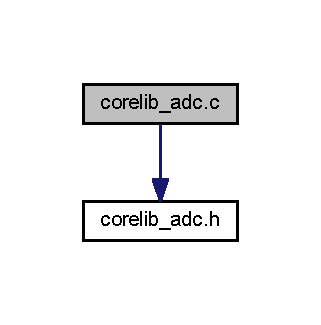
\includegraphics[width=154pt]{corelib__adc_8c__incl}
\end{center}
\end{figure}
\subsection*{Functions}
\begin{DoxyCompactItemize}
\item 
void {\bf setup\-A\-D\-C} (void)
\item 
void {\bf setup\-A\-D\-C\-Pins\-To\-Digital} (void)
\item 
void {\bf adc\-Set\-Channel} (unsigned char uc\-Channel)
\item 
float {\bf adc\-Read\-Only} (void)
\item 
void {\bf adc\-Start} (void)
\item 
void {\bf adc\-Set\-Vref} (float Vref)
\end{DoxyCompactItemize}


\subsection{Function Documentation}
\index{corelib\-\_\-adc.\-c@{corelib\-\_\-adc.\-c}!adc\-Read\-Only@{adc\-Read\-Only}}
\index{adc\-Read\-Only@{adc\-Read\-Only}!corelib_adc.c@{corelib\-\_\-adc.\-c}}
\subsubsection[{adc\-Read\-Only}]{\setlength{\rightskip}{0pt plus 5cm}float adc\-Read\-Only (
\begin{DoxyParamCaption}
\item[{void}]{}
\end{DoxyParamCaption}
)}\label{corelib__adc_8c_ac8b3feac26439e9b19303931e7f9a268}


Definition at line 119 of file corelib\-\_\-adc.\-c.

\index{corelib\-\_\-adc.\-c@{corelib\-\_\-adc.\-c}!adc\-Set\-Channel@{adc\-Set\-Channel}}
\index{adc\-Set\-Channel@{adc\-Set\-Channel}!corelib_adc.c@{corelib\-\_\-adc.\-c}}
\subsubsection[{adc\-Set\-Channel}]{\setlength{\rightskip}{0pt plus 5cm}void adc\-Set\-Channel (
\begin{DoxyParamCaption}
\item[{unsigned char}]{uc\-Channel}
\end{DoxyParamCaption}
)}\label{corelib__adc_8c_a91365887a1a86d19034945a79b08567c}


Definition at line 91 of file corelib\-\_\-adc.\-c.

\index{corelib\-\_\-adc.\-c@{corelib\-\_\-adc.\-c}!adc\-Set\-Vref@{adc\-Set\-Vref}}
\index{adc\-Set\-Vref@{adc\-Set\-Vref}!corelib_adc.c@{corelib\-\_\-adc.\-c}}
\subsubsection[{adc\-Set\-Vref}]{\setlength{\rightskip}{0pt plus 5cm}void adc\-Set\-Vref (
\begin{DoxyParamCaption}
\item[{float}]{Vref}
\end{DoxyParamCaption}
)}\label{corelib__adc_8c_a399f78b6f492b8f00550315d39ae641d}


Definition at line 137 of file corelib\-\_\-adc.\-c.

\index{corelib\-\_\-adc.\-c@{corelib\-\_\-adc.\-c}!adc\-Start@{adc\-Start}}
\index{adc\-Start@{adc\-Start}!corelib_adc.c@{corelib\-\_\-adc.\-c}}
\subsubsection[{adc\-Start}]{\setlength{\rightskip}{0pt plus 5cm}void adc\-Start (
\begin{DoxyParamCaption}
\item[{void}]{}
\end{DoxyParamCaption}
)}\label{corelib__adc_8c_a716f2932005a7a9b55d077cb3c177ca2}


Definition at line 127 of file corelib\-\_\-adc.\-c.

\index{corelib\-\_\-adc.\-c@{corelib\-\_\-adc.\-c}!setup\-A\-D\-C@{setup\-A\-D\-C}}
\index{setup\-A\-D\-C@{setup\-A\-D\-C}!corelib_adc.c@{corelib\-\_\-adc.\-c}}
\subsubsection[{setup\-A\-D\-C}]{\setlength{\rightskip}{0pt plus 5cm}void setup\-A\-D\-C (
\begin{DoxyParamCaption}
\item[{void}]{}
\end{DoxyParamCaption}
)}\label{corelib__adc_8c_abd26438ee5b31bb1a8d2e808336d4301}


Definition at line 46 of file corelib\-\_\-adc.\-c.

\index{corelib\-\_\-adc.\-c@{corelib\-\_\-adc.\-c}!setup\-A\-D\-C\-Pins\-To\-Digital@{setup\-A\-D\-C\-Pins\-To\-Digital}}
\index{setup\-A\-D\-C\-Pins\-To\-Digital@{setup\-A\-D\-C\-Pins\-To\-Digital}!corelib_adc.c@{corelib\-\_\-adc.\-c}}
\subsubsection[{setup\-A\-D\-C\-Pins\-To\-Digital}]{\setlength{\rightskip}{0pt plus 5cm}void setup\-A\-D\-C\-Pins\-To\-Digital (
\begin{DoxyParamCaption}
\item[{void}]{}
\end{DoxyParamCaption}
)}\label{corelib__adc_8c_a03e1cf9150f81b0626da03d64efcf011}


Definition at line 82 of file corelib\-\_\-adc.\-c.


\section{corelib\-\_\-adc.\-h File Reference}
\label{corelib__adc_8h}\index{corelib\-\_\-adc.\-h@{corelib\-\_\-adc.\-h}}
This graph shows which files directly or indirectly include this file\-:\nopagebreak
\begin{figure}[H]
\begin{center}
\leavevmode
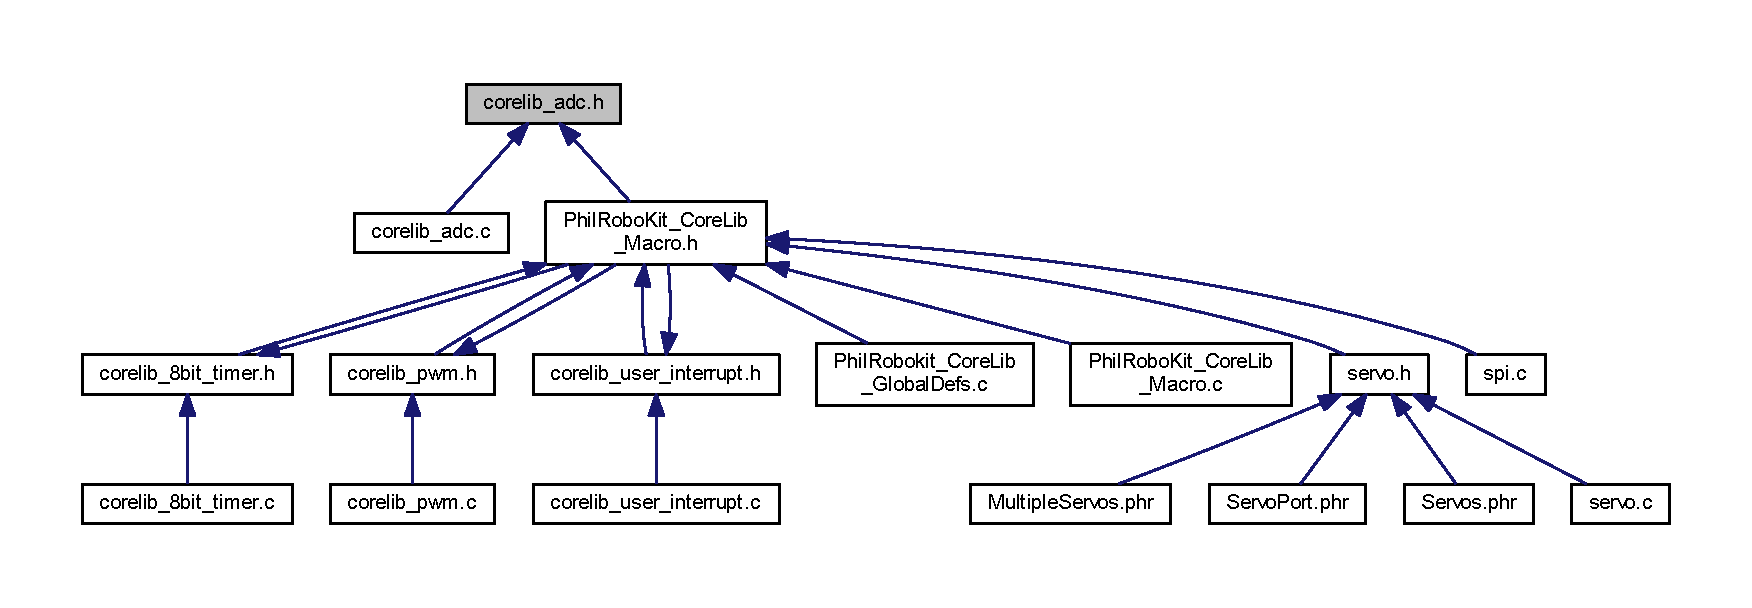
\includegraphics[width=350pt]{corelib__adc_8h__dep__incl}
\end{center}
\end{figure}
\subsection*{Macros}
\begin{DoxyCompactItemize}
\item 
\#define {\bf is\-A\-D\-C\-Conversion\-Done}()~({\bf B\-I\-T\-\_\-\-A\-D\-C\-O\-N0\-\_\-\-G\-O\-\_\-\-D\-O\-N\-E}? 0\-: 1)
\end{DoxyCompactItemize}
\subsection*{Functions}
\begin{DoxyCompactItemize}
\item 
void {\bf setup\-A\-D\-C} (void)
\item 
void {\bf setup\-A\-D\-C\-Pins\-To\-Digital} (void)
\item 
void {\bf adc\-Start} (void)
\item 
void {\bf adc\-Set\-Channel} (unsigned char uc\-Channel)
\item 
float {\bf adc\-Read\-Only} (void)
\item 
void {\bf adc\-Set\-Vref} (float Vref)
\end{DoxyCompactItemize}


\subsection{Macro Definition Documentation}
\index{corelib\-\_\-adc.\-h@{corelib\-\_\-adc.\-h}!is\-A\-D\-C\-Conversion\-Done@{is\-A\-D\-C\-Conversion\-Done}}
\index{is\-A\-D\-C\-Conversion\-Done@{is\-A\-D\-C\-Conversion\-Done}!corelib_adc.h@{corelib\-\_\-adc.\-h}}
\subsubsection[{is\-A\-D\-C\-Conversion\-Done}]{\setlength{\rightskip}{0pt plus 5cm}\#define is\-A\-D\-C\-Conversion\-Done(
\begin{DoxyParamCaption}
{}
\end{DoxyParamCaption}
)~({\bf B\-I\-T\-\_\-\-A\-D\-C\-O\-N0\-\_\-\-G\-O\-\_\-\-D\-O\-N\-E}? 0\-: 1)}\label{corelib__adc_8h_a9e8fa1458f9015483c979ccdbb5a0bcf}


Definition at line 53 of file corelib\-\_\-adc.\-h.



\subsection{Function Documentation}
\index{corelib\-\_\-adc.\-h@{corelib\-\_\-adc.\-h}!adc\-Read\-Only@{adc\-Read\-Only}}
\index{adc\-Read\-Only@{adc\-Read\-Only}!corelib_adc.h@{corelib\-\_\-adc.\-h}}
\subsubsection[{adc\-Read\-Only}]{\setlength{\rightskip}{0pt plus 5cm}float adc\-Read\-Only (
\begin{DoxyParamCaption}
\item[{void}]{}
\end{DoxyParamCaption}
)}\label{corelib__adc_8h_ac8b3feac26439e9b19303931e7f9a268}


Definition at line 119 of file corelib\-\_\-adc.\-c.

\index{corelib\-\_\-adc.\-h@{corelib\-\_\-adc.\-h}!adc\-Set\-Channel@{adc\-Set\-Channel}}
\index{adc\-Set\-Channel@{adc\-Set\-Channel}!corelib_adc.h@{corelib\-\_\-adc.\-h}}
\subsubsection[{adc\-Set\-Channel}]{\setlength{\rightskip}{0pt plus 5cm}void adc\-Set\-Channel (
\begin{DoxyParamCaption}
\item[{unsigned char}]{uc\-Channel}
\end{DoxyParamCaption}
)}\label{corelib__adc_8h_a91365887a1a86d19034945a79b08567c}


Definition at line 91 of file corelib\-\_\-adc.\-c.

\index{corelib\-\_\-adc.\-h@{corelib\-\_\-adc.\-h}!adc\-Set\-Vref@{adc\-Set\-Vref}}
\index{adc\-Set\-Vref@{adc\-Set\-Vref}!corelib_adc.h@{corelib\-\_\-adc.\-h}}
\subsubsection[{adc\-Set\-Vref}]{\setlength{\rightskip}{0pt plus 5cm}void adc\-Set\-Vref (
\begin{DoxyParamCaption}
\item[{float}]{Vref}
\end{DoxyParamCaption}
)}\label{corelib__adc_8h_a399f78b6f492b8f00550315d39ae641d}


Definition at line 137 of file corelib\-\_\-adc.\-c.

\index{corelib\-\_\-adc.\-h@{corelib\-\_\-adc.\-h}!adc\-Start@{adc\-Start}}
\index{adc\-Start@{adc\-Start}!corelib_adc.h@{corelib\-\_\-adc.\-h}}
\subsubsection[{adc\-Start}]{\setlength{\rightskip}{0pt plus 5cm}void adc\-Start (
\begin{DoxyParamCaption}
\item[{void}]{}
\end{DoxyParamCaption}
)}\label{corelib__adc_8h_a716f2932005a7a9b55d077cb3c177ca2}


Definition at line 127 of file corelib\-\_\-adc.\-c.

\index{corelib\-\_\-adc.\-h@{corelib\-\_\-adc.\-h}!setup\-A\-D\-C@{setup\-A\-D\-C}}
\index{setup\-A\-D\-C@{setup\-A\-D\-C}!corelib_adc.h@{corelib\-\_\-adc.\-h}}
\subsubsection[{setup\-A\-D\-C}]{\setlength{\rightskip}{0pt plus 5cm}void setup\-A\-D\-C (
\begin{DoxyParamCaption}
\item[{void}]{}
\end{DoxyParamCaption}
)}\label{corelib__adc_8h_abd26438ee5b31bb1a8d2e808336d4301}


Definition at line 46 of file corelib\-\_\-adc.\-c.

\index{corelib\-\_\-adc.\-h@{corelib\-\_\-adc.\-h}!setup\-A\-D\-C\-Pins\-To\-Digital@{setup\-A\-D\-C\-Pins\-To\-Digital}}
\index{setup\-A\-D\-C\-Pins\-To\-Digital@{setup\-A\-D\-C\-Pins\-To\-Digital}!corelib_adc.h@{corelib\-\_\-adc.\-h}}
\subsubsection[{setup\-A\-D\-C\-Pins\-To\-Digital}]{\setlength{\rightskip}{0pt plus 5cm}void setup\-A\-D\-C\-Pins\-To\-Digital (
\begin{DoxyParamCaption}
\item[{void}]{}
\end{DoxyParamCaption}
)}\label{corelib__adc_8h_a03e1cf9150f81b0626da03d64efcf011}


Definition at line 82 of file corelib\-\_\-adc.\-c.


\section{corelib\-\_\-pwm.\-c File Reference}
\label{corelib__pwm_8c}\index{corelib\-\_\-pwm.\-c@{corelib\-\_\-pwm.\-c}}
{\ttfamily \#include \char`\"{}corelib\-\_\-pwm.\-h\char`\"{}}\\*
Include dependency graph for corelib\-\_\-pwm.\-c\-:\nopagebreak
\begin{figure}[H]
\begin{center}
\leavevmode
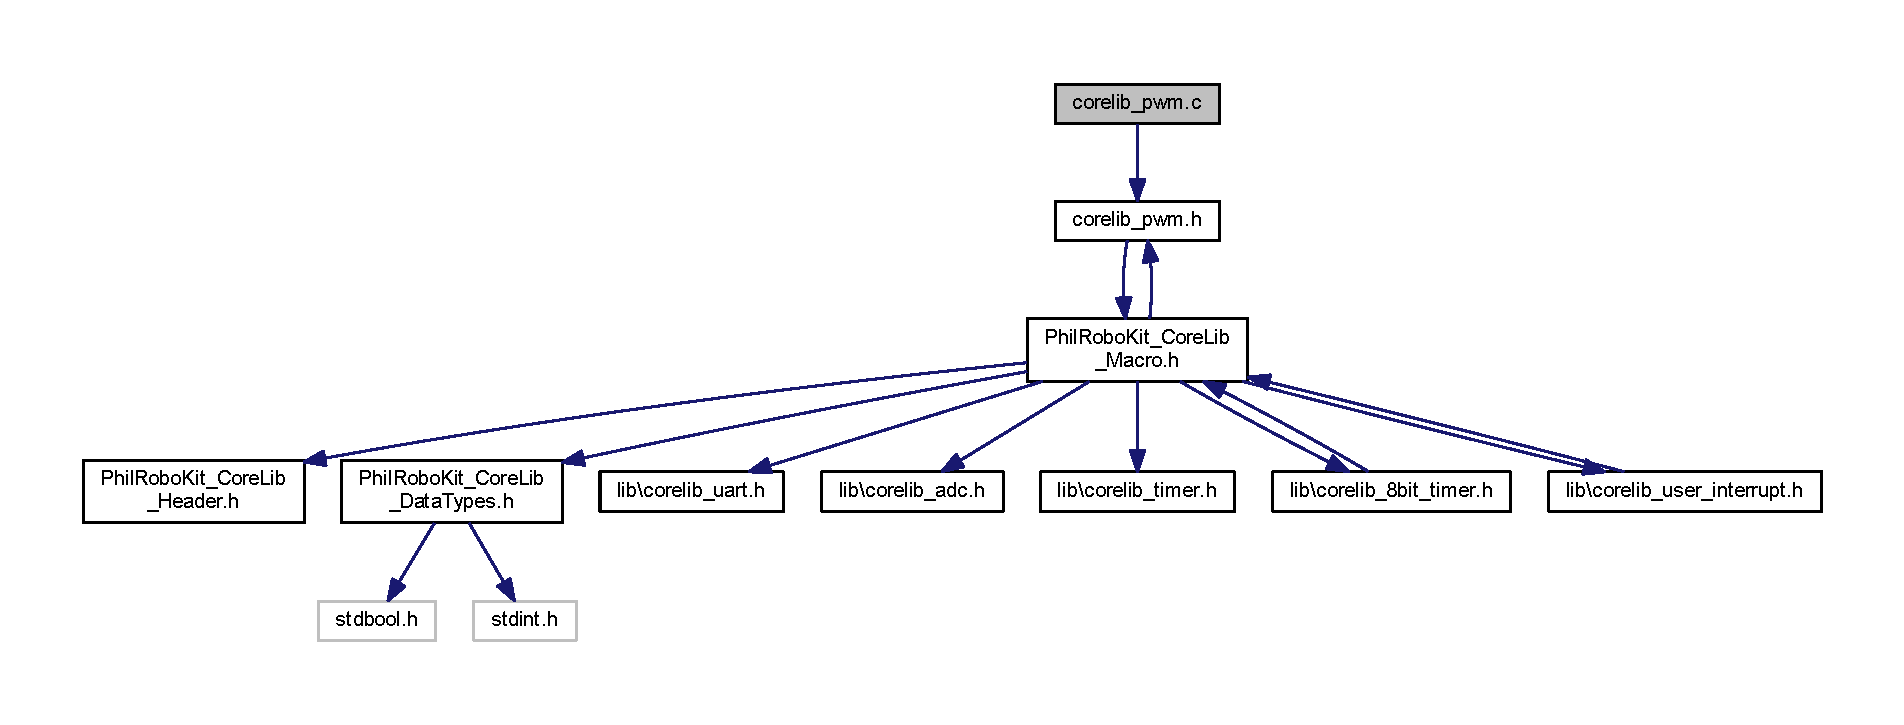
\includegraphics[width=350pt]{corelib__pwm_8c__incl}
\end{center}
\end{figure}
\subsection*{Functions}
\begin{DoxyCompactItemize}
\item 
void {\bf set\-P\-W\-M\-Frequency} (uint16\-\_\-t ui16\-Frequency)
\item 
void {\bf set\-P\-W\-M\-Duty} (enum {\bf e\-P\-W\-M\-Modules} e\-P\-W\-M\-\_\-\-Module, uint16\-\_\-t ui16\-Duty\-Cycle)
\item 
void {\bf setup\-P\-W\-M} (enum {\bf e\-P\-W\-M\-Modules} e\-P\-W\-M\-\_\-\-Module, uint16\-\_\-t ui16\-Frequency, uint16\-\_\-t ui16\-Duty\-Cycle)
\item 
void {\bf set\-Analog\-Out} (enum {\bf e\-P\-W\-M\-Modules} e\-D\-A\-C\-\_\-\-Module, uint16\-\_\-t ui16\-Value)
\item 
void {\bf remove\-Analog\-Out} (enum {\bf e\-P\-W\-M\-Modules} e\-D\-A\-C\-\_\-\-Module)
\item 
void {\bf remove\-P\-W\-M} (enum {\bf e\-P\-W\-M\-Modules} e\-P\-W\-M\-\_\-\-Module)
\end{DoxyCompactItemize}


\subsection{Function Documentation}
\index{corelib\-\_\-pwm.\-c@{corelib\-\_\-pwm.\-c}!remove\-Analog\-Out@{remove\-Analog\-Out}}
\index{remove\-Analog\-Out@{remove\-Analog\-Out}!corelib_pwm.c@{corelib\-\_\-pwm.\-c}}
\subsubsection[{remove\-Analog\-Out}]{\setlength{\rightskip}{0pt plus 5cm}void remove\-Analog\-Out (
\begin{DoxyParamCaption}
\item[{enum {\bf e\-P\-W\-M\-Modules}}]{e\-D\-A\-C\-\_\-\-Module}
\end{DoxyParamCaption}
)}\label{corelib__pwm_8c_af28b8a69190fdf2709585f9e36bd98d4}


Definition at line 194 of file corelib\-\_\-pwm.\-c.



Here is the call graph for this function\-:\nopagebreak
\begin{figure}[H]
\begin{center}
\leavevmode
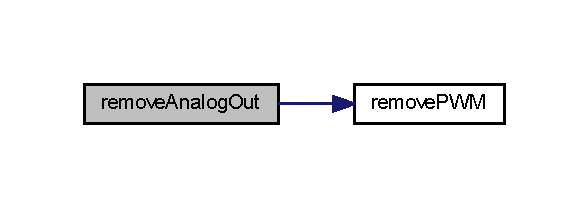
\includegraphics[width=282pt]{corelib__pwm_8c_af28b8a69190fdf2709585f9e36bd98d4_cgraph}
\end{center}
\end{figure}


\index{corelib\-\_\-pwm.\-c@{corelib\-\_\-pwm.\-c}!remove\-P\-W\-M@{remove\-P\-W\-M}}
\index{remove\-P\-W\-M@{remove\-P\-W\-M}!corelib_pwm.c@{corelib\-\_\-pwm.\-c}}
\subsubsection[{remove\-P\-W\-M}]{\setlength{\rightskip}{0pt plus 5cm}void remove\-P\-W\-M (
\begin{DoxyParamCaption}
\item[{enum {\bf e\-P\-W\-M\-Modules}}]{e\-P\-W\-M\-\_\-\-Module}
\end{DoxyParamCaption}
)}\label{corelib__pwm_8c_a0c549ab97a20654a43590a51ba61f706}


Definition at line 199 of file corelib\-\_\-pwm.\-c.

\index{corelib\-\_\-pwm.\-c@{corelib\-\_\-pwm.\-c}!set\-Analog\-Out@{set\-Analog\-Out}}
\index{set\-Analog\-Out@{set\-Analog\-Out}!corelib_pwm.c@{corelib\-\_\-pwm.\-c}}
\subsubsection[{set\-Analog\-Out}]{\setlength{\rightskip}{0pt plus 5cm}void set\-Analog\-Out (
\begin{DoxyParamCaption}
\item[{enum {\bf e\-P\-W\-M\-Modules}}]{e\-D\-A\-C\-\_\-\-Module, }
\item[{uint16\-\_\-t}]{ui16\-Value}
\end{DoxyParamCaption}
)}\label{corelib__pwm_8c_acbef1791f4d3d135da66a88b1f69988b}


Definition at line 184 of file corelib\-\_\-pwm.\-c.



Here is the call graph for this function\-:\nopagebreak
\begin{figure}[H]
\begin{center}
\leavevmode
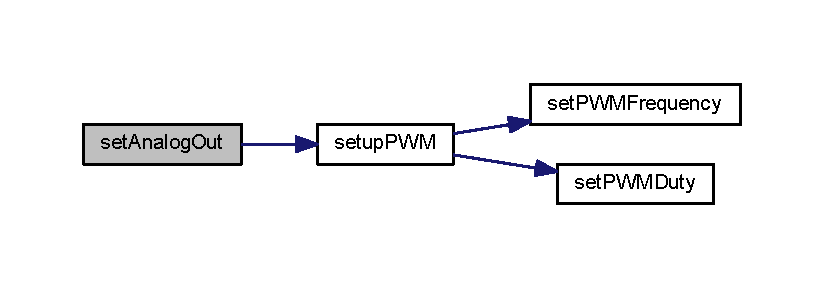
\includegraphics[width=350pt]{corelib__pwm_8c_acbef1791f4d3d135da66a88b1f69988b_cgraph}
\end{center}
\end{figure}


\index{corelib\-\_\-pwm.\-c@{corelib\-\_\-pwm.\-c}!set\-P\-W\-M\-Duty@{set\-P\-W\-M\-Duty}}
\index{set\-P\-W\-M\-Duty@{set\-P\-W\-M\-Duty}!corelib_pwm.c@{corelib\-\_\-pwm.\-c}}
\subsubsection[{set\-P\-W\-M\-Duty}]{\setlength{\rightskip}{0pt plus 5cm}void set\-P\-W\-M\-Duty (
\begin{DoxyParamCaption}
\item[{enum {\bf e\-P\-W\-M\-Modules}}]{e\-P\-W\-M\-\_\-\-Module, }
\item[{uint16\-\_\-t}]{ui16\-Duty\-Cycle}
\end{DoxyParamCaption}
)}\label{corelib__pwm_8c_a27c205e7d1e45f5bdb245bd38c23d51e}


Definition at line 115 of file corelib\-\_\-pwm.\-c.

\index{corelib\-\_\-pwm.\-c@{corelib\-\_\-pwm.\-c}!set\-P\-W\-M\-Frequency@{set\-P\-W\-M\-Frequency}}
\index{set\-P\-W\-M\-Frequency@{set\-P\-W\-M\-Frequency}!corelib_pwm.c@{corelib\-\_\-pwm.\-c}}
\subsubsection[{set\-P\-W\-M\-Frequency}]{\setlength{\rightskip}{0pt plus 5cm}void set\-P\-W\-M\-Frequency (
\begin{DoxyParamCaption}
\item[{uint16\-\_\-t}]{ui16\-Frequency}
\end{DoxyParamCaption}
)}\label{corelib__pwm_8c_ad30cbd98de04abc5d58ec540df5a04fc}


Definition at line 52 of file corelib\-\_\-pwm.\-c.

\index{corelib\-\_\-pwm.\-c@{corelib\-\_\-pwm.\-c}!setup\-P\-W\-M@{setup\-P\-W\-M}}
\index{setup\-P\-W\-M@{setup\-P\-W\-M}!corelib_pwm.c@{corelib\-\_\-pwm.\-c}}
\subsubsection[{setup\-P\-W\-M}]{\setlength{\rightskip}{0pt plus 5cm}void setup\-P\-W\-M (
\begin{DoxyParamCaption}
\item[{enum {\bf e\-P\-W\-M\-Modules}}]{e\-P\-W\-M\-\_\-\-Module, }
\item[{uint16\-\_\-t}]{ui16\-Frequency, }
\item[{uint16\-\_\-t}]{ui16\-Duty\-Cycle}
\end{DoxyParamCaption}
)}\label{corelib__pwm_8c_a21481afa7d76f35cb0bb0140613352e4}


Definition at line 144 of file corelib\-\_\-pwm.\-c.



Here is the call graph for this function\-:\nopagebreak
\begin{figure}[H]
\begin{center}
\leavevmode
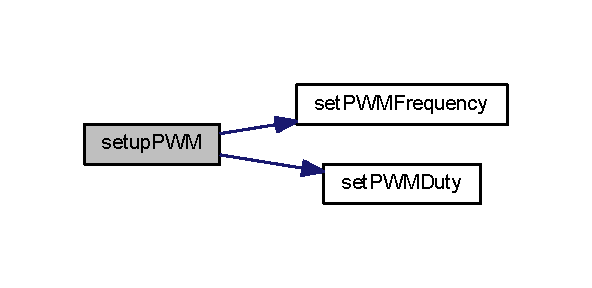
\includegraphics[width=284pt]{corelib__pwm_8c_a21481afa7d76f35cb0bb0140613352e4_cgraph}
\end{center}
\end{figure}



\section{corelib\-\_\-pwm.\-h File Reference}
\label{corelib__pwm_8h}\index{corelib\-\_\-pwm.\-h@{corelib\-\_\-pwm.\-h}}
{\ttfamily \#include $<$Phil\-Robo\-Kit\-\_\-\-Core\-Lib\-\_\-\-Macro.\-h$>$}\\*
Include dependency graph for corelib\-\_\-pwm.\-h\-:\nopagebreak
\begin{figure}[H]
\begin{center}
\leavevmode
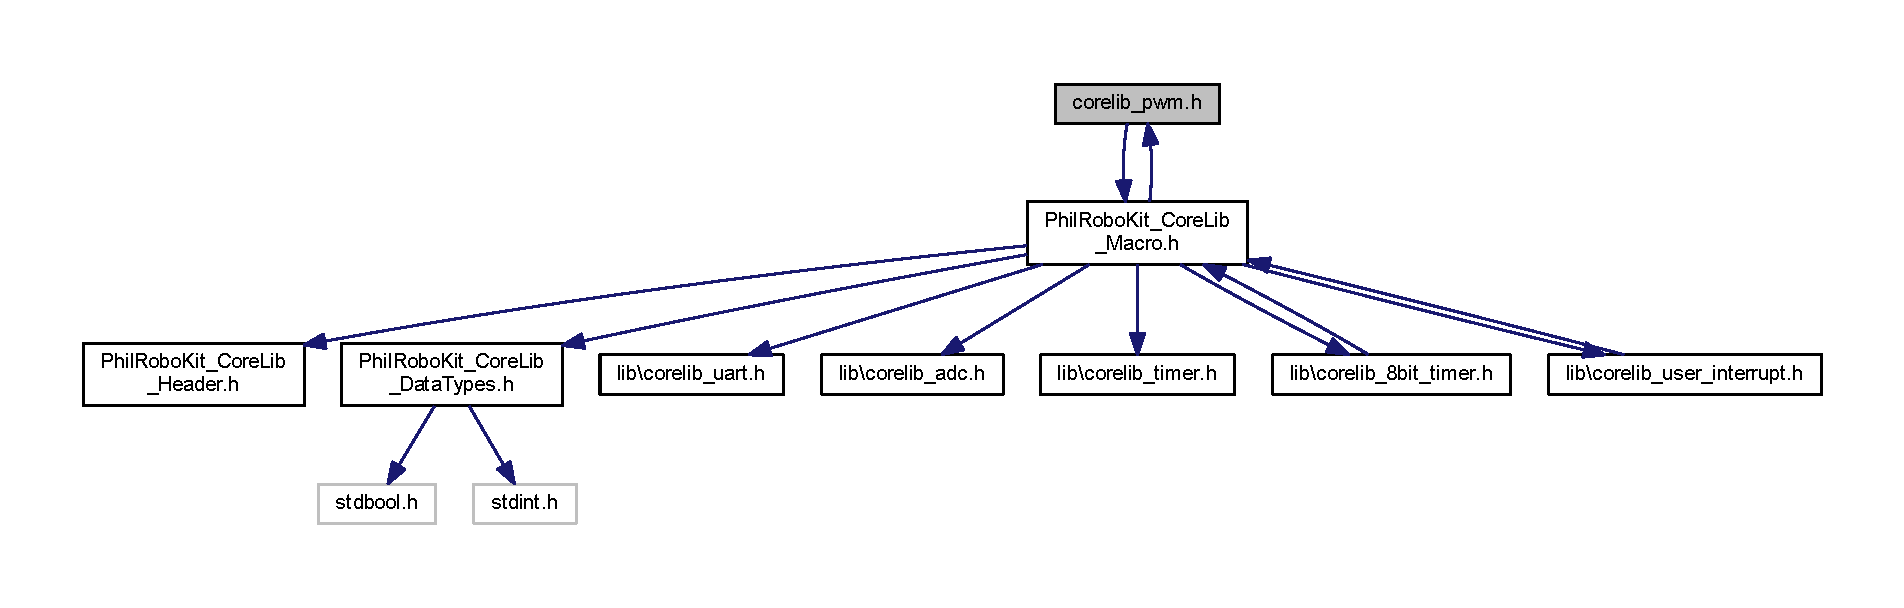
\includegraphics[width=350pt]{corelib__pwm_8h__incl}
\end{center}
\end{figure}
This graph shows which files directly or indirectly include this file\-:\nopagebreak
\begin{figure}[H]
\begin{center}
\leavevmode
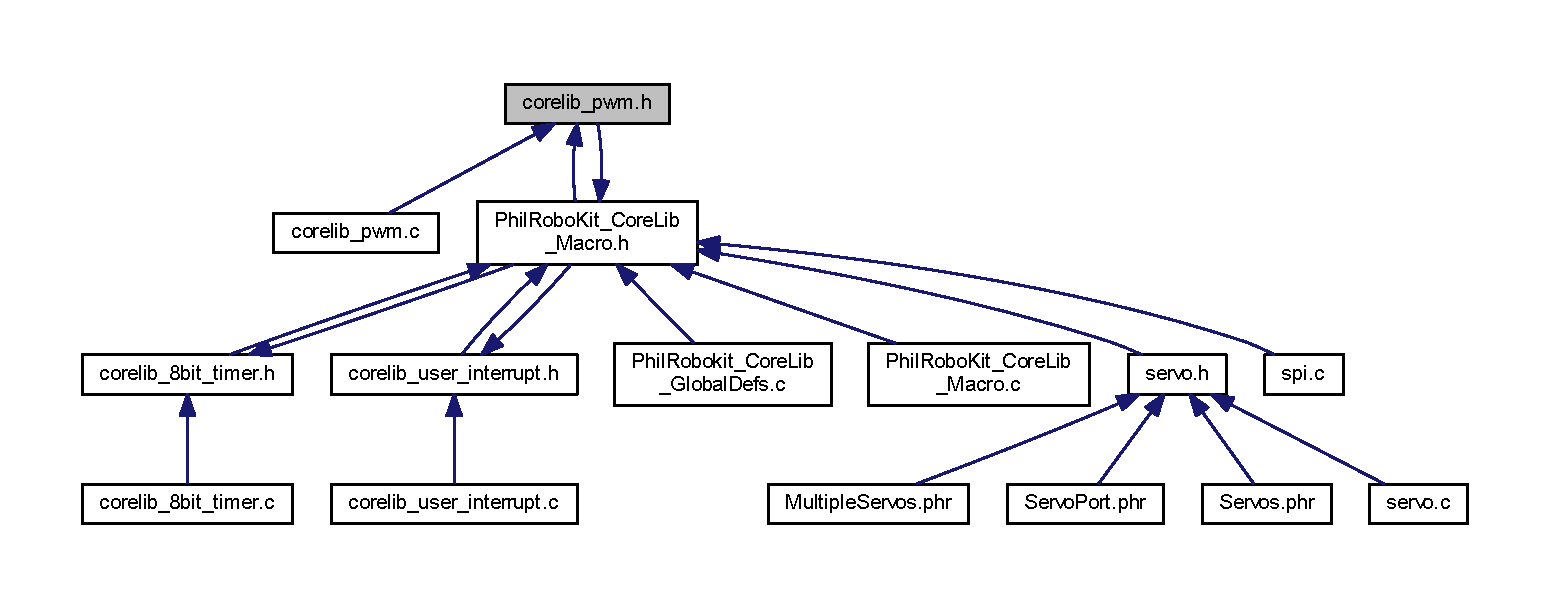
\includegraphics[width=350pt]{corelib__pwm_8h__dep__incl}
\end{center}
\end{figure}
\subsection*{Macros}
\begin{DoxyCompactItemize}
\item 
\#define {\bf D\-A\-C0}~{\bf P\-W\-M0}
\item 
\#define {\bf D\-A\-C1}~{\bf P\-W\-M1}
\item 
\#define {\bf C\-C\-P\-\_\-\-P\-W\-M\-\_\-\-M\-O\-D\-E}~{\bf P\-W\-M\-\_\-\-M\-O\-D\-E}
\item 
\#define {\bf mc\-\_\-\-P\-W\-M\-Timer\-Int\-En}()~{\bf mc\-\_\-timer2\-Int\-En}()
\item 
\#define {\bf mc\-\_\-\-P\-W\-M\-Timer\-Int\-Dis}()~{\bf mc\-\_\-timer2\-Int\-Dis}()
\item 
\#define {\bf mc\-\_\-\-P\-W\-M\-Timer\-I\-F\-Clr}()~{\bf mc\-\_\-timer2\-I\-F\-Clr}()
\item 
\#define {\bf mc\-\_\-\-Enable\-P\-W\-M\-Tmr}()~{\bf mc\-\_\-enable\-T\-M\-R2}()
\item 
\#define {\bf mc\-\_\-\-Disable\-P\-W\-M\-Tmr}()~{\bf mc\-\_\-disable\-T\-M\-R2}()
\item 
\#define {\bf mc\-\_\-config\-C\-C\-P1\-Mode}(a)~{\bf R\-E\-G\-I\-S\-T\-E\-R\-\_\-\-C\-C\-P1\-C\-O\-N} = a\&{\bf C\-C\-P\-\_\-\-M\-O\-D\-E\-\_\-\-M\-A\-S\-K}
\item 
\#define {\bf mc\-\_\-config\-C\-C\-P2\-Mode}(a)~{\bf R\-E\-G\-I\-S\-T\-E\-R\-\_\-\-C\-C\-P2\-C\-O\-N} = a\&{\bf C\-C\-P\-\_\-\-M\-O\-D\-E\-\_\-\-M\-A\-S\-K}
\item 
\#define {\bf mc\-\_\-set\-P\-W\-M0\-\_\-\-On}()~{\bf mc\-\_\-config\-C\-C\-P1\-Mode}({\bf P\-W\-M\-\_\-\-M\-O\-D\-E});
\item 
\#define {\bf mc\-\_\-set\-P\-W\-M0\-\_\-\-Off}()~{\bf mc\-\_\-config\-C\-C\-P1\-Mode}({\bf P\-W\-M\-\_\-\-O\-F\-F});
\item 
\#define {\bf mc\-\_\-set\-P\-W\-M1\-\_\-\-On}()~{\bf mc\-\_\-config\-C\-C\-P2\-Mode}({\bf P\-W\-M\-\_\-\-M\-O\-D\-E});
\item 
\#define {\bf mc\-\_\-set\-P\-W\-M1\-\_\-\-Off}()~{\bf mc\-\_\-config\-C\-C\-P2\-Mode}({\bf P\-W\-M\-\_\-\-O\-F\-F});
\item 
\#define {\bf mc\-\_\-\-P\-W\-M\-Timer\-\_\-\-Init}(a)~{\bf setup8\-Bit\-Timer}({\bf T\-I\-M\-E\-R2},a,0)
\item 
\#define {\bf mc\-\_\-set\-P\-W\-M\-Period}(a)~{\bf set\-Timer\-Value}({\bf T\-I\-M\-E\-R2},a)
\item 
\#define {\bf mc\-\_\-set\-P\-W\-M0\-Ton}(a)
\item 
\#define {\bf mc\-\_\-set\-P\-W\-M1\-Ton}(a)
\end{DoxyCompactItemize}
\subsection*{Enumerations}
\begin{DoxyCompactItemize}
\item 
enum {\bf e\-P\-W\-M\-Modules} \{ {\bf P\-W\-M0}, 
{\bf P\-W\-M1}
 \}
\item 
enum {\bf e\-P\-W\-M\-Modes} \{ \\*
{\bf P\-W\-M\-\_\-\-O\-F\-F} =  0x00, 
{\bf C\-O\-M\-P\-\_\-\-T\-O\-G\-G\-L\-E\-\_\-\-C\-C\-P\-O} =  0x02, 
{\bf C\-A\-P\-T\-U\-R\-E\-\_\-\-F\-A\-L\-L} =  0x04, 
{\bf C\-A\-P\-T\-U\-R\-E\-\_\-\-R\-I\-S\-E} =  0x05, 
\\*
{\bf C\-A\-P\-T\-U\-R\-E\-\_\-4\-T\-H\-\_\-\-F\-A\-L\-L} =  0x06, 
{\bf C\-A\-P\-T\-U\-R\-E\-\_\-16\-T\-H\-\_\-\-R\-I\-S\-E} =  0x07, 
{\bf P\-W\-M\-\_\-\-M\-O\-D\-E} =  0x0\-C
 \}
\end{DoxyCompactItemize}
\subsection*{Functions}
\begin{DoxyCompactItemize}
\item 
void {\bf setup\-P\-W\-M} (enum {\bf e\-P\-W\-M\-Modules} e\-P\-W\-M\-\_\-\-Module, uint16\-\_\-t ui16\-Frequency, uint16\-\_\-t ui16\-Duty\-Cycle)
\item 
void {\bf set\-P\-W\-M\-Frequency} (uint16\-\_\-t ui16\-Frequency)
\item 
void {\bf set\-P\-W\-M\-Duty} (enum {\bf e\-P\-W\-M\-Modules} e\-P\-W\-M\-\_\-\-Module, uint16\-\_\-t ui16\-Duty\-Cycle)
\item 
void {\bf remove\-P\-W\-M} (enum {\bf e\-P\-W\-M\-Modules} e\-P\-W\-M\-\_\-\-Module)
\item 
void {\bf set\-Analog\-Out} (enum {\bf e\-P\-W\-M\-Modules} e\-D\-A\-C\-\_\-\-Module, uint16\-\_\-t ui16\-Value)
\item 
void {\bf remove\-Analog\-Out} (enum {\bf e\-P\-W\-M\-Modules} e\-D\-A\-C\-\_\-\-Module)
\end{DoxyCompactItemize}


\subsection{Macro Definition Documentation}
\index{corelib\-\_\-pwm.\-h@{corelib\-\_\-pwm.\-h}!C\-C\-P\-\_\-\-P\-W\-M\-\_\-\-M\-O\-D\-E@{C\-C\-P\-\_\-\-P\-W\-M\-\_\-\-M\-O\-D\-E}}
\index{C\-C\-P\-\_\-\-P\-W\-M\-\_\-\-M\-O\-D\-E@{C\-C\-P\-\_\-\-P\-W\-M\-\_\-\-M\-O\-D\-E}!corelib_pwm.h@{corelib\-\_\-pwm.\-h}}
\subsubsection[{C\-C\-P\-\_\-\-P\-W\-M\-\_\-\-M\-O\-D\-E}]{\setlength{\rightskip}{0pt plus 5cm}\#define C\-C\-P\-\_\-\-P\-W\-M\-\_\-\-M\-O\-D\-E~{\bf P\-W\-M\-\_\-\-M\-O\-D\-E}}\label{corelib__pwm_8h_ac360f480cfde33db8392547be6ee2bc9}


Definition at line 79 of file corelib\-\_\-pwm.\-h.

\index{corelib\-\_\-pwm.\-h@{corelib\-\_\-pwm.\-h}!D\-A\-C0@{D\-A\-C0}}
\index{D\-A\-C0@{D\-A\-C0}!corelib_pwm.h@{corelib\-\_\-pwm.\-h}}
\subsubsection[{D\-A\-C0}]{\setlength{\rightskip}{0pt plus 5cm}\#define D\-A\-C0~{\bf P\-W\-M0}}\label{corelib__pwm_8h_adfe0025fe66918c644e110c3b055c955}


Definition at line 61 of file corelib\-\_\-pwm.\-h.

\index{corelib\-\_\-pwm.\-h@{corelib\-\_\-pwm.\-h}!D\-A\-C1@{D\-A\-C1}}
\index{D\-A\-C1@{D\-A\-C1}!corelib_pwm.h@{corelib\-\_\-pwm.\-h}}
\subsubsection[{D\-A\-C1}]{\setlength{\rightskip}{0pt plus 5cm}\#define D\-A\-C1~{\bf P\-W\-M1}}\label{corelib__pwm_8h_affb5ff8779fa698f3c7165a617d56e4f}


Definition at line 62 of file corelib\-\_\-pwm.\-h.

\index{corelib\-\_\-pwm.\-h@{corelib\-\_\-pwm.\-h}!mc\-\_\-config\-C\-C\-P1\-Mode@{mc\-\_\-config\-C\-C\-P1\-Mode}}
\index{mc\-\_\-config\-C\-C\-P1\-Mode@{mc\-\_\-config\-C\-C\-P1\-Mode}!corelib_pwm.h@{corelib\-\_\-pwm.\-h}}
\subsubsection[{mc\-\_\-config\-C\-C\-P1\-Mode}]{\setlength{\rightskip}{0pt plus 5cm}\#define mc\-\_\-config\-C\-C\-P1\-Mode(
\begin{DoxyParamCaption}
\item[{}]{a}
\end{DoxyParamCaption}
)~{\bf R\-E\-G\-I\-S\-T\-E\-R\-\_\-\-C\-C\-P1\-C\-O\-N} = a\&{\bf C\-C\-P\-\_\-\-M\-O\-D\-E\-\_\-\-M\-A\-S\-K}}\label{corelib__pwm_8h_a78bf3c6004f792de8090235ef6f3b9ee}


Definition at line 101 of file corelib\-\_\-pwm.\-h.

\index{corelib\-\_\-pwm.\-h@{corelib\-\_\-pwm.\-h}!mc\-\_\-config\-C\-C\-P2\-Mode@{mc\-\_\-config\-C\-C\-P2\-Mode}}
\index{mc\-\_\-config\-C\-C\-P2\-Mode@{mc\-\_\-config\-C\-C\-P2\-Mode}!corelib_pwm.h@{corelib\-\_\-pwm.\-h}}
\subsubsection[{mc\-\_\-config\-C\-C\-P2\-Mode}]{\setlength{\rightskip}{0pt plus 5cm}\#define mc\-\_\-config\-C\-C\-P2\-Mode(
\begin{DoxyParamCaption}
\item[{}]{a}
\end{DoxyParamCaption}
)~{\bf R\-E\-G\-I\-S\-T\-E\-R\-\_\-\-C\-C\-P2\-C\-O\-N} = a\&{\bf C\-C\-P\-\_\-\-M\-O\-D\-E\-\_\-\-M\-A\-S\-K}}\label{corelib__pwm_8h_a3434882bab79cf0630d184625c34fd22}


Definition at line 104 of file corelib\-\_\-pwm.\-h.

\index{corelib\-\_\-pwm.\-h@{corelib\-\_\-pwm.\-h}!mc\-\_\-\-Disable\-P\-W\-M\-Tmr@{mc\-\_\-\-Disable\-P\-W\-M\-Tmr}}
\index{mc\-\_\-\-Disable\-P\-W\-M\-Tmr@{mc\-\_\-\-Disable\-P\-W\-M\-Tmr}!corelib_pwm.h@{corelib\-\_\-pwm.\-h}}
\subsubsection[{mc\-\_\-\-Disable\-P\-W\-M\-Tmr}]{\setlength{\rightskip}{0pt plus 5cm}\#define mc\-\_\-\-Disable\-P\-W\-M\-Tmr(
\begin{DoxyParamCaption}
{}
\end{DoxyParamCaption}
)~{\bf mc\-\_\-disable\-T\-M\-R2}()}\label{corelib__pwm_8h_addb7f485cd1e6c599a8037b92913e27d}


Definition at line 99 of file corelib\-\_\-pwm.\-h.

\index{corelib\-\_\-pwm.\-h@{corelib\-\_\-pwm.\-h}!mc\-\_\-\-Enable\-P\-W\-M\-Tmr@{mc\-\_\-\-Enable\-P\-W\-M\-Tmr}}
\index{mc\-\_\-\-Enable\-P\-W\-M\-Tmr@{mc\-\_\-\-Enable\-P\-W\-M\-Tmr}!corelib_pwm.h@{corelib\-\_\-pwm.\-h}}
\subsubsection[{mc\-\_\-\-Enable\-P\-W\-M\-Tmr}]{\setlength{\rightskip}{0pt plus 5cm}\#define mc\-\_\-\-Enable\-P\-W\-M\-Tmr(
\begin{DoxyParamCaption}
{}
\end{DoxyParamCaption}
)~{\bf mc\-\_\-enable\-T\-M\-R2}()}\label{corelib__pwm_8h_a5d66695ca5af5c07b0f4a18f301d1d1a}


Definition at line 98 of file corelib\-\_\-pwm.\-h.

\index{corelib\-\_\-pwm.\-h@{corelib\-\_\-pwm.\-h}!mc\-\_\-\-P\-W\-M\-Timer\-\_\-\-Init@{mc\-\_\-\-P\-W\-M\-Timer\-\_\-\-Init}}
\index{mc\-\_\-\-P\-W\-M\-Timer\-\_\-\-Init@{mc\-\_\-\-P\-W\-M\-Timer\-\_\-\-Init}!corelib_pwm.h@{corelib\-\_\-pwm.\-h}}
\subsubsection[{mc\-\_\-\-P\-W\-M\-Timer\-\_\-\-Init}]{\setlength{\rightskip}{0pt plus 5cm}\#define mc\-\_\-\-P\-W\-M\-Timer\-\_\-\-Init(
\begin{DoxyParamCaption}
\item[{}]{a}
\end{DoxyParamCaption}
)~{\bf setup8\-Bit\-Timer}({\bf T\-I\-M\-E\-R2},a,0)}\label{corelib__pwm_8h_aacd1c8895939bf3d5b152c2112cf6100}


Definition at line 123 of file corelib\-\_\-pwm.\-h.

\index{corelib\-\_\-pwm.\-h@{corelib\-\_\-pwm.\-h}!mc\-\_\-\-P\-W\-M\-Timer\-I\-F\-Clr@{mc\-\_\-\-P\-W\-M\-Timer\-I\-F\-Clr}}
\index{mc\-\_\-\-P\-W\-M\-Timer\-I\-F\-Clr@{mc\-\_\-\-P\-W\-M\-Timer\-I\-F\-Clr}!corelib_pwm.h@{corelib\-\_\-pwm.\-h}}
\subsubsection[{mc\-\_\-\-P\-W\-M\-Timer\-I\-F\-Clr}]{\setlength{\rightskip}{0pt plus 5cm}\#define mc\-\_\-\-P\-W\-M\-Timer\-I\-F\-Clr(
\begin{DoxyParamCaption}
{}
\end{DoxyParamCaption}
)~{\bf mc\-\_\-timer2\-I\-F\-Clr}()}\label{corelib__pwm_8h_aa4381c22db0c13a3c1ed7c0a3a7d74a3}


Definition at line 96 of file corelib\-\_\-pwm.\-h.

\index{corelib\-\_\-pwm.\-h@{corelib\-\_\-pwm.\-h}!mc\-\_\-\-P\-W\-M\-Timer\-Int\-Dis@{mc\-\_\-\-P\-W\-M\-Timer\-Int\-Dis}}
\index{mc\-\_\-\-P\-W\-M\-Timer\-Int\-Dis@{mc\-\_\-\-P\-W\-M\-Timer\-Int\-Dis}!corelib_pwm.h@{corelib\-\_\-pwm.\-h}}
\subsubsection[{mc\-\_\-\-P\-W\-M\-Timer\-Int\-Dis}]{\setlength{\rightskip}{0pt plus 5cm}\#define mc\-\_\-\-P\-W\-M\-Timer\-Int\-Dis(
\begin{DoxyParamCaption}
{}
\end{DoxyParamCaption}
)~{\bf mc\-\_\-timer2\-Int\-Dis}()}\label{corelib__pwm_8h_a887e6f0073aced33ac69b12185a1ecc6}


Definition at line 95 of file corelib\-\_\-pwm.\-h.

\index{corelib\-\_\-pwm.\-h@{corelib\-\_\-pwm.\-h}!mc\-\_\-\-P\-W\-M\-Timer\-Int\-En@{mc\-\_\-\-P\-W\-M\-Timer\-Int\-En}}
\index{mc\-\_\-\-P\-W\-M\-Timer\-Int\-En@{mc\-\_\-\-P\-W\-M\-Timer\-Int\-En}!corelib_pwm.h@{corelib\-\_\-pwm.\-h}}
\subsubsection[{mc\-\_\-\-P\-W\-M\-Timer\-Int\-En}]{\setlength{\rightskip}{0pt plus 5cm}\#define mc\-\_\-\-P\-W\-M\-Timer\-Int\-En(
\begin{DoxyParamCaption}
{}
\end{DoxyParamCaption}
)~{\bf mc\-\_\-timer2\-Int\-En}()}\label{corelib__pwm_8h_a5ea4853bff66fc720f2aab00f46686d2}


Definition at line 94 of file corelib\-\_\-pwm.\-h.

\index{corelib\-\_\-pwm.\-h@{corelib\-\_\-pwm.\-h}!mc\-\_\-set\-P\-W\-M0\-\_\-\-Off@{mc\-\_\-set\-P\-W\-M0\-\_\-\-Off}}
\index{mc\-\_\-set\-P\-W\-M0\-\_\-\-Off@{mc\-\_\-set\-P\-W\-M0\-\_\-\-Off}!corelib_pwm.h@{corelib\-\_\-pwm.\-h}}
\subsubsection[{mc\-\_\-set\-P\-W\-M0\-\_\-\-Off}]{\setlength{\rightskip}{0pt plus 5cm}\#define mc\-\_\-set\-P\-W\-M0\-\_\-\-Off(
\begin{DoxyParamCaption}
{}
\end{DoxyParamCaption}
)~{\bf mc\-\_\-config\-C\-C\-P1\-Mode}({\bf P\-W\-M\-\_\-\-O\-F\-F});}\label{corelib__pwm_8h_a8308316bc0968fdf532703d5af07cbdb}


Definition at line 111 of file corelib\-\_\-pwm.\-h.

\index{corelib\-\_\-pwm.\-h@{corelib\-\_\-pwm.\-h}!mc\-\_\-set\-P\-W\-M0\-\_\-\-On@{mc\-\_\-set\-P\-W\-M0\-\_\-\-On}}
\index{mc\-\_\-set\-P\-W\-M0\-\_\-\-On@{mc\-\_\-set\-P\-W\-M0\-\_\-\-On}!corelib_pwm.h@{corelib\-\_\-pwm.\-h}}
\subsubsection[{mc\-\_\-set\-P\-W\-M0\-\_\-\-On}]{\setlength{\rightskip}{0pt plus 5cm}\#define mc\-\_\-set\-P\-W\-M0\-\_\-\-On(
\begin{DoxyParamCaption}
{}
\end{DoxyParamCaption}
)~{\bf mc\-\_\-config\-C\-C\-P1\-Mode}({\bf P\-W\-M\-\_\-\-M\-O\-D\-E});}\label{corelib__pwm_8h_a82946d85050eb117a9001bb76bc240b0}


Definition at line 107 of file corelib\-\_\-pwm.\-h.

\index{corelib\-\_\-pwm.\-h@{corelib\-\_\-pwm.\-h}!mc\-\_\-set\-P\-W\-M0\-Ton@{mc\-\_\-set\-P\-W\-M0\-Ton}}
\index{mc\-\_\-set\-P\-W\-M0\-Ton@{mc\-\_\-set\-P\-W\-M0\-Ton}!corelib_pwm.h@{corelib\-\_\-pwm.\-h}}
\subsubsection[{mc\-\_\-set\-P\-W\-M0\-Ton}]{\setlength{\rightskip}{0pt plus 5cm}\#define mc\-\_\-set\-P\-W\-M0\-Ton(
\begin{DoxyParamCaption}
\item[{}]{a}
\end{DoxyParamCaption}
)}\label{corelib__pwm_8h_aa641e26d101dcced4ecbfebcfb435feb}
{\bfseries Value\-:}
\begin{DoxyCode}
REGISTER_CCP1CON &= ~PWM_DC_LSB_MASK;   \(\backslash\)
    REGISTER\_CCP1CON |= (a&0x0003)<<4;      \(\backslash\)
    REGISTER\_CCPR1L = (a&0x03FC)>>2
\end{DoxyCode}


Definition at line 126 of file corelib\-\_\-pwm.\-h.

\index{corelib\-\_\-pwm.\-h@{corelib\-\_\-pwm.\-h}!mc\-\_\-set\-P\-W\-M1\-\_\-\-Off@{mc\-\_\-set\-P\-W\-M1\-\_\-\-Off}}
\index{mc\-\_\-set\-P\-W\-M1\-\_\-\-Off@{mc\-\_\-set\-P\-W\-M1\-\_\-\-Off}!corelib_pwm.h@{corelib\-\_\-pwm.\-h}}
\subsubsection[{mc\-\_\-set\-P\-W\-M1\-\_\-\-Off}]{\setlength{\rightskip}{0pt plus 5cm}\#define mc\-\_\-set\-P\-W\-M1\-\_\-\-Off(
\begin{DoxyParamCaption}
{}
\end{DoxyParamCaption}
)~{\bf mc\-\_\-config\-C\-C\-P2\-Mode}({\bf P\-W\-M\-\_\-\-O\-F\-F});}\label{corelib__pwm_8h_a57680580e13685e77d9f1fd50417ddac}


Definition at line 119 of file corelib\-\_\-pwm.\-h.

\index{corelib\-\_\-pwm.\-h@{corelib\-\_\-pwm.\-h}!mc\-\_\-set\-P\-W\-M1\-\_\-\-On@{mc\-\_\-set\-P\-W\-M1\-\_\-\-On}}
\index{mc\-\_\-set\-P\-W\-M1\-\_\-\-On@{mc\-\_\-set\-P\-W\-M1\-\_\-\-On}!corelib_pwm.h@{corelib\-\_\-pwm.\-h}}
\subsubsection[{mc\-\_\-set\-P\-W\-M1\-\_\-\-On}]{\setlength{\rightskip}{0pt plus 5cm}\#define mc\-\_\-set\-P\-W\-M1\-\_\-\-On(
\begin{DoxyParamCaption}
{}
\end{DoxyParamCaption}
)~{\bf mc\-\_\-config\-C\-C\-P2\-Mode}({\bf P\-W\-M\-\_\-\-M\-O\-D\-E});}\label{corelib__pwm_8h_aabb6449a94f06e1cc954d65b91663f08}


Definition at line 115 of file corelib\-\_\-pwm.\-h.

\index{corelib\-\_\-pwm.\-h@{corelib\-\_\-pwm.\-h}!mc\-\_\-set\-P\-W\-M1\-Ton@{mc\-\_\-set\-P\-W\-M1\-Ton}}
\index{mc\-\_\-set\-P\-W\-M1\-Ton@{mc\-\_\-set\-P\-W\-M1\-Ton}!corelib_pwm.h@{corelib\-\_\-pwm.\-h}}
\subsubsection[{mc\-\_\-set\-P\-W\-M1\-Ton}]{\setlength{\rightskip}{0pt plus 5cm}\#define mc\-\_\-set\-P\-W\-M1\-Ton(
\begin{DoxyParamCaption}
\item[{}]{a}
\end{DoxyParamCaption}
)}\label{corelib__pwm_8h_aec2cae4085a744b3774713e5729b2957}
{\bfseries Value\-:}
\begin{DoxyCode}
REGISTER_CCP2CON &= ~PWM_DC_LSB_MASK;   \(\backslash\)
    REGISTER\_CCP2CON |= (a&0x0003)<<4;      \(\backslash\)
    REGISTER\_CCPR2L = (a&0x03FC)>>2
\end{DoxyCode}


Definition at line 130 of file corelib\-\_\-pwm.\-h.

\index{corelib\-\_\-pwm.\-h@{corelib\-\_\-pwm.\-h}!mc\-\_\-set\-P\-W\-M\-Period@{mc\-\_\-set\-P\-W\-M\-Period}}
\index{mc\-\_\-set\-P\-W\-M\-Period@{mc\-\_\-set\-P\-W\-M\-Period}!corelib_pwm.h@{corelib\-\_\-pwm.\-h}}
\subsubsection[{mc\-\_\-set\-P\-W\-M\-Period}]{\setlength{\rightskip}{0pt plus 5cm}\#define mc\-\_\-set\-P\-W\-M\-Period(
\begin{DoxyParamCaption}
\item[{}]{a}
\end{DoxyParamCaption}
)~{\bf set\-Timer\-Value}({\bf T\-I\-M\-E\-R2},a)}\label{corelib__pwm_8h_a290f5deacb52284fed8b63bcc801d1d8}


Definition at line 125 of file corelib\-\_\-pwm.\-h.



\subsection{Enumeration Type Documentation}
\index{corelib\-\_\-pwm.\-h@{corelib\-\_\-pwm.\-h}!e\-P\-W\-M\-Modes@{e\-P\-W\-M\-Modes}}
\index{e\-P\-W\-M\-Modes@{e\-P\-W\-M\-Modes}!corelib_pwm.h@{corelib\-\_\-pwm.\-h}}
\subsubsection[{e\-P\-W\-M\-Modes}]{\setlength{\rightskip}{0pt plus 5cm}enum {\bf e\-P\-W\-M\-Modes}}\label{corelib__pwm_8h_a451f0b8686340890e1bfcfe19089833d}
\begin{Desc}
\item[Enumerator\-: ]\par
\begin{description}
\index{P\-W\-M\-\_\-\-O\-F\-F@{P\-W\-M\-\_\-\-O\-F\-F}!corelib\-\_\-pwm.\-h@{corelib\-\_\-pwm.\-h}}\index{corelib\-\_\-pwm.\-h@{corelib\-\_\-pwm.\-h}!P\-W\-M\-\_\-\-O\-F\-F@{P\-W\-M\-\_\-\-O\-F\-F}}\item[{\em 
P\-W\-M\-\_\-\-O\-F\-F\label{corelib__pwm_8h_a451f0b8686340890e1bfcfe19089833da4b87f8b5b8f76b141c7a22d2c95e0ecb}
}]\index{C\-O\-M\-P\-\_\-\-T\-O\-G\-G\-L\-E\-\_\-\-C\-C\-P\-O@{C\-O\-M\-P\-\_\-\-T\-O\-G\-G\-L\-E\-\_\-\-C\-C\-P\-O}!corelib\-\_\-pwm.\-h@{corelib\-\_\-pwm.\-h}}\index{corelib\-\_\-pwm.\-h@{corelib\-\_\-pwm.\-h}!C\-O\-M\-P\-\_\-\-T\-O\-G\-G\-L\-E\-\_\-\-C\-C\-P\-O@{C\-O\-M\-P\-\_\-\-T\-O\-G\-G\-L\-E\-\_\-\-C\-C\-P\-O}}\item[{\em 
C\-O\-M\-P\-\_\-\-T\-O\-G\-G\-L\-E\-\_\-\-C\-C\-P\-O\label{corelib__pwm_8h_a451f0b8686340890e1bfcfe19089833da082ed5ba6d803da087a6595f9b63d18f}
}]\index{C\-A\-P\-T\-U\-R\-E\-\_\-\-F\-A\-L\-L@{C\-A\-P\-T\-U\-R\-E\-\_\-\-F\-A\-L\-L}!corelib\-\_\-pwm.\-h@{corelib\-\_\-pwm.\-h}}\index{corelib\-\_\-pwm.\-h@{corelib\-\_\-pwm.\-h}!C\-A\-P\-T\-U\-R\-E\-\_\-\-F\-A\-L\-L@{C\-A\-P\-T\-U\-R\-E\-\_\-\-F\-A\-L\-L}}\item[{\em 
C\-A\-P\-T\-U\-R\-E\-\_\-\-F\-A\-L\-L\label{corelib__pwm_8h_a451f0b8686340890e1bfcfe19089833da7e52f19e2d2538bde3caac8e948f38e7}
}]\index{C\-A\-P\-T\-U\-R\-E\-\_\-\-R\-I\-S\-E@{C\-A\-P\-T\-U\-R\-E\-\_\-\-R\-I\-S\-E}!corelib\-\_\-pwm.\-h@{corelib\-\_\-pwm.\-h}}\index{corelib\-\_\-pwm.\-h@{corelib\-\_\-pwm.\-h}!C\-A\-P\-T\-U\-R\-E\-\_\-\-R\-I\-S\-E@{C\-A\-P\-T\-U\-R\-E\-\_\-\-R\-I\-S\-E}}\item[{\em 
C\-A\-P\-T\-U\-R\-E\-\_\-\-R\-I\-S\-E\label{corelib__pwm_8h_a451f0b8686340890e1bfcfe19089833dade10ec968a8cd24412fa887fdd7acd8c}
}]\index{C\-A\-P\-T\-U\-R\-E\-\_\-4\-T\-H\-\_\-\-F\-A\-L\-L@{C\-A\-P\-T\-U\-R\-E\-\_\-4\-T\-H\-\_\-\-F\-A\-L\-L}!corelib\-\_\-pwm.\-h@{corelib\-\_\-pwm.\-h}}\index{corelib\-\_\-pwm.\-h@{corelib\-\_\-pwm.\-h}!C\-A\-P\-T\-U\-R\-E\-\_\-4\-T\-H\-\_\-\-F\-A\-L\-L@{C\-A\-P\-T\-U\-R\-E\-\_\-4\-T\-H\-\_\-\-F\-A\-L\-L}}\item[{\em 
C\-A\-P\-T\-U\-R\-E\-\_\-4\-T\-H\-\_\-\-F\-A\-L\-L\label{corelib__pwm_8h_a451f0b8686340890e1bfcfe19089833da1b6c765177dec9bf2f4b49da4f232489}
}]\index{C\-A\-P\-T\-U\-R\-E\-\_\-16\-T\-H\-\_\-\-R\-I\-S\-E@{C\-A\-P\-T\-U\-R\-E\-\_\-16\-T\-H\-\_\-\-R\-I\-S\-E}!corelib\-\_\-pwm.\-h@{corelib\-\_\-pwm.\-h}}\index{corelib\-\_\-pwm.\-h@{corelib\-\_\-pwm.\-h}!C\-A\-P\-T\-U\-R\-E\-\_\-16\-T\-H\-\_\-\-R\-I\-S\-E@{C\-A\-P\-T\-U\-R\-E\-\_\-16\-T\-H\-\_\-\-R\-I\-S\-E}}\item[{\em 
C\-A\-P\-T\-U\-R\-E\-\_\-16\-T\-H\-\_\-\-R\-I\-S\-E\label{corelib__pwm_8h_a451f0b8686340890e1bfcfe19089833da84e7672799da93eebb08f649b6212389}
}]\index{P\-W\-M\-\_\-\-M\-O\-D\-E@{P\-W\-M\-\_\-\-M\-O\-D\-E}!corelib\-\_\-pwm.\-h@{corelib\-\_\-pwm.\-h}}\index{corelib\-\_\-pwm.\-h@{corelib\-\_\-pwm.\-h}!P\-W\-M\-\_\-\-M\-O\-D\-E@{P\-W\-M\-\_\-\-M\-O\-D\-E}}\item[{\em 
P\-W\-M\-\_\-\-M\-O\-D\-E\label{corelib__pwm_8h_a451f0b8686340890e1bfcfe19089833da6ddb3b94e3599054126d1f65cd1109f3}
}]\end{description}
\end{Desc}



Definition at line 65 of file corelib\-\_\-pwm.\-h.

\index{corelib\-\_\-pwm.\-h@{corelib\-\_\-pwm.\-h}!e\-P\-W\-M\-Modules@{e\-P\-W\-M\-Modules}}
\index{e\-P\-W\-M\-Modules@{e\-P\-W\-M\-Modules}!corelib_pwm.h@{corelib\-\_\-pwm.\-h}}
\subsubsection[{e\-P\-W\-M\-Modules}]{\setlength{\rightskip}{0pt plus 5cm}enum {\bf e\-P\-W\-M\-Modules}}\label{corelib__pwm_8h_a438983ad60cd20801958dc7bcc00e903}
\begin{Desc}
\item[Enumerator\-: ]\par
\begin{description}
\index{P\-W\-M0@{P\-W\-M0}!corelib\-\_\-pwm.\-h@{corelib\-\_\-pwm.\-h}}\index{corelib\-\_\-pwm.\-h@{corelib\-\_\-pwm.\-h}!P\-W\-M0@{P\-W\-M0}}\item[{\em 
P\-W\-M0\label{corelib__pwm_8h_a438983ad60cd20801958dc7bcc00e903a4969f4b49dd00aa89aa0b6b3a7cce0cc}
}]\index{P\-W\-M1@{P\-W\-M1}!corelib\-\_\-pwm.\-h@{corelib\-\_\-pwm.\-h}}\index{corelib\-\_\-pwm.\-h@{corelib\-\_\-pwm.\-h}!P\-W\-M1@{P\-W\-M1}}\item[{\em 
P\-W\-M1\label{corelib__pwm_8h_a438983ad60cd20801958dc7bcc00e903acc6ab0fb66c5ba52524e32ea2ad0bd1a}
}]\end{description}
\end{Desc}



Definition at line 55 of file corelib\-\_\-pwm.\-h.



\subsection{Function Documentation}
\index{corelib\-\_\-pwm.\-h@{corelib\-\_\-pwm.\-h}!remove\-Analog\-Out@{remove\-Analog\-Out}}
\index{remove\-Analog\-Out@{remove\-Analog\-Out}!corelib_pwm.h@{corelib\-\_\-pwm.\-h}}
\subsubsection[{remove\-Analog\-Out}]{\setlength{\rightskip}{0pt plus 5cm}void remove\-Analog\-Out (
\begin{DoxyParamCaption}
\item[{enum {\bf e\-P\-W\-M\-Modules}}]{e\-D\-A\-C\-\_\-\-Module}
\end{DoxyParamCaption}
)}\label{corelib__pwm_8h_af28b8a69190fdf2709585f9e36bd98d4}


Definition at line 194 of file corelib\-\_\-pwm.\-c.



Here is the call graph for this function\-:\nopagebreak
\begin{figure}[H]
\begin{center}
\leavevmode
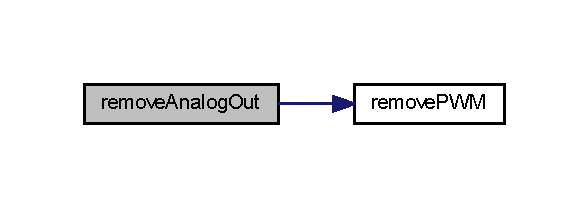
\includegraphics[width=282pt]{corelib__pwm_8h_af28b8a69190fdf2709585f9e36bd98d4_cgraph}
\end{center}
\end{figure}


\index{corelib\-\_\-pwm.\-h@{corelib\-\_\-pwm.\-h}!remove\-P\-W\-M@{remove\-P\-W\-M}}
\index{remove\-P\-W\-M@{remove\-P\-W\-M}!corelib_pwm.h@{corelib\-\_\-pwm.\-h}}
\subsubsection[{remove\-P\-W\-M}]{\setlength{\rightskip}{0pt plus 5cm}void remove\-P\-W\-M (
\begin{DoxyParamCaption}
\item[{enum {\bf e\-P\-W\-M\-Modules}}]{e\-P\-W\-M\-\_\-\-Module}
\end{DoxyParamCaption}
)}\label{corelib__pwm_8h_a0c549ab97a20654a43590a51ba61f706}


Definition at line 199 of file corelib\-\_\-pwm.\-c.

\index{corelib\-\_\-pwm.\-h@{corelib\-\_\-pwm.\-h}!set\-Analog\-Out@{set\-Analog\-Out}}
\index{set\-Analog\-Out@{set\-Analog\-Out}!corelib_pwm.h@{corelib\-\_\-pwm.\-h}}
\subsubsection[{set\-Analog\-Out}]{\setlength{\rightskip}{0pt plus 5cm}void set\-Analog\-Out (
\begin{DoxyParamCaption}
\item[{enum {\bf e\-P\-W\-M\-Modules}}]{e\-D\-A\-C\-\_\-\-Module, }
\item[{uint16\-\_\-t}]{ui16\-Value}
\end{DoxyParamCaption}
)}\label{corelib__pwm_8h_acbef1791f4d3d135da66a88b1f69988b}


Definition at line 184 of file corelib\-\_\-pwm.\-c.



Here is the call graph for this function\-:\nopagebreak
\begin{figure}[H]
\begin{center}
\leavevmode
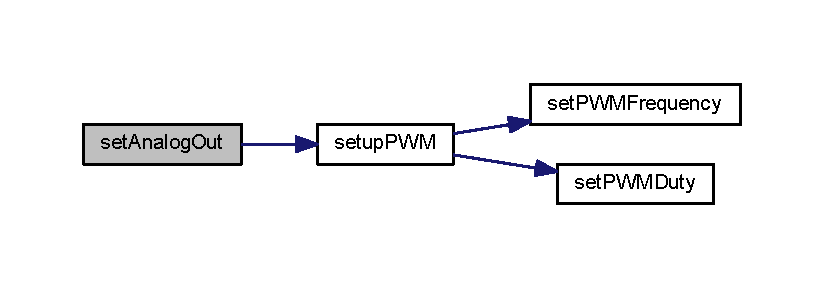
\includegraphics[width=350pt]{corelib__pwm_8h_acbef1791f4d3d135da66a88b1f69988b_cgraph}
\end{center}
\end{figure}


\index{corelib\-\_\-pwm.\-h@{corelib\-\_\-pwm.\-h}!set\-P\-W\-M\-Duty@{set\-P\-W\-M\-Duty}}
\index{set\-P\-W\-M\-Duty@{set\-P\-W\-M\-Duty}!corelib_pwm.h@{corelib\-\_\-pwm.\-h}}
\subsubsection[{set\-P\-W\-M\-Duty}]{\setlength{\rightskip}{0pt plus 5cm}void set\-P\-W\-M\-Duty (
\begin{DoxyParamCaption}
\item[{enum {\bf e\-P\-W\-M\-Modules}}]{e\-P\-W\-M\-\_\-\-Module, }
\item[{uint16\-\_\-t}]{ui16\-Duty\-Cycle}
\end{DoxyParamCaption}
)}\label{corelib__pwm_8h_a27c205e7d1e45f5bdb245bd38c23d51e}


Definition at line 115 of file corelib\-\_\-pwm.\-c.

\index{corelib\-\_\-pwm.\-h@{corelib\-\_\-pwm.\-h}!set\-P\-W\-M\-Frequency@{set\-P\-W\-M\-Frequency}}
\index{set\-P\-W\-M\-Frequency@{set\-P\-W\-M\-Frequency}!corelib_pwm.h@{corelib\-\_\-pwm.\-h}}
\subsubsection[{set\-P\-W\-M\-Frequency}]{\setlength{\rightskip}{0pt plus 5cm}void set\-P\-W\-M\-Frequency (
\begin{DoxyParamCaption}
\item[{uint16\-\_\-t}]{ui16\-Frequency}
\end{DoxyParamCaption}
)}\label{corelib__pwm_8h_ad30cbd98de04abc5d58ec540df5a04fc}


Definition at line 52 of file corelib\-\_\-pwm.\-c.

\index{corelib\-\_\-pwm.\-h@{corelib\-\_\-pwm.\-h}!setup\-P\-W\-M@{setup\-P\-W\-M}}
\index{setup\-P\-W\-M@{setup\-P\-W\-M}!corelib_pwm.h@{corelib\-\_\-pwm.\-h}}
\subsubsection[{setup\-P\-W\-M}]{\setlength{\rightskip}{0pt plus 5cm}void setup\-P\-W\-M (
\begin{DoxyParamCaption}
\item[{enum {\bf e\-P\-W\-M\-Modules}}]{e\-P\-W\-M\-\_\-\-Module, }
\item[{uint16\-\_\-t}]{ui16\-Frequency, }
\item[{uint16\-\_\-t}]{ui16\-Duty\-Cycle}
\end{DoxyParamCaption}
)}\label{corelib__pwm_8h_a21481afa7d76f35cb0bb0140613352e4}


Definition at line 144 of file corelib\-\_\-pwm.\-c.



Here is the call graph for this function\-:\nopagebreak
\begin{figure}[H]
\begin{center}
\leavevmode
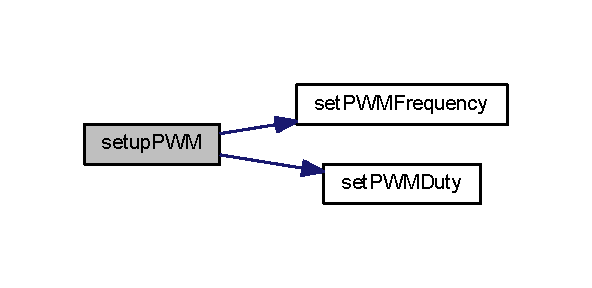
\includegraphics[width=284pt]{corelib__pwm_8h_a21481afa7d76f35cb0bb0140613352e4_cgraph}
\end{center}
\end{figure}



\section{corelib\-\_\-timer.\-c File Reference}
\label{corelib__timer_8c}\index{corelib\-\_\-timer.\-c@{corelib\-\_\-timer.\-c}}
{\ttfamily \#include \char`\"{}corelib\-\_\-timer.\-h\char`\"{}}\\*
Include dependency graph for corelib\-\_\-timer.\-c\-:\nopagebreak
\begin{figure}[H]
\begin{center}
\leavevmode
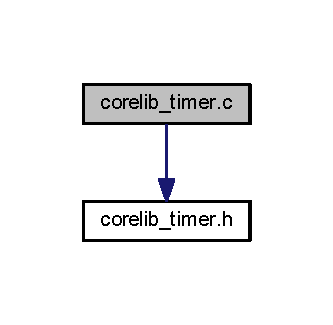
\includegraphics[width=160pt]{corelib__timer_8c__incl}
\end{center}
\end{figure}
\subsection*{Functions}
\begin{DoxyCompactItemize}
\item 
void {\bf timer\-Interrupt\-Handler} (void)
\item 
void {\bf timer\-Init} (void)
\item 
unsigned int {\bf get\-Elapsed\-Time\-Ms} (unsigned int ui\-Time\-Ms)
\item 
unsigned int {\bf get\-Time\-Ms} (void)
\item 
unsigned int {\bf get\-Elapsed\-Time\-Us} (unsigned int ui\-Time\-Us)
\item 
unsigned int {\bf get\-Time\-Us} (void)
\end{DoxyCompactItemize}


\subsection{Function Documentation}
\index{corelib\-\_\-timer.\-c@{corelib\-\_\-timer.\-c}!get\-Elapsed\-Time\-Ms@{get\-Elapsed\-Time\-Ms}}
\index{get\-Elapsed\-Time\-Ms@{get\-Elapsed\-Time\-Ms}!corelib_timer.c@{corelib\-\_\-timer.\-c}}
\subsubsection[{get\-Elapsed\-Time\-Ms}]{\setlength{\rightskip}{0pt plus 5cm}unsigned int get\-Elapsed\-Time\-Ms (
\begin{DoxyParamCaption}
\item[{unsigned int}]{ui\-Time\-Ms}
\end{DoxyParamCaption}
)}\label{corelib__timer_8c_acf72cf4216df47fd55b2b68944acd8e7}


Definition at line 83 of file corelib\-\_\-timer.\-c.

\index{corelib\-\_\-timer.\-c@{corelib\-\_\-timer.\-c}!get\-Elapsed\-Time\-Us@{get\-Elapsed\-Time\-Us}}
\index{get\-Elapsed\-Time\-Us@{get\-Elapsed\-Time\-Us}!corelib_timer.c@{corelib\-\_\-timer.\-c}}
\subsubsection[{get\-Elapsed\-Time\-Us}]{\setlength{\rightskip}{0pt plus 5cm}unsigned int get\-Elapsed\-Time\-Us (
\begin{DoxyParamCaption}
\item[{unsigned int}]{ui\-Time\-Us}
\end{DoxyParamCaption}
)}\label{corelib__timer_8c_a0493c088a76d2d3ab4037d3f8ddcdb96}


Definition at line 93 of file corelib\-\_\-timer.\-c.

\index{corelib\-\_\-timer.\-c@{corelib\-\_\-timer.\-c}!get\-Time\-Ms@{get\-Time\-Ms}}
\index{get\-Time\-Ms@{get\-Time\-Ms}!corelib_timer.c@{corelib\-\_\-timer.\-c}}
\subsubsection[{get\-Time\-Ms}]{\setlength{\rightskip}{0pt plus 5cm}unsigned int get\-Time\-Ms (
\begin{DoxyParamCaption}
\item[{void}]{}
\end{DoxyParamCaption}
)}\label{corelib__timer_8c_ae9bfb9f90b70aa56cee9f098bc432af9}


Definition at line 88 of file corelib\-\_\-timer.\-c.

\index{corelib\-\_\-timer.\-c@{corelib\-\_\-timer.\-c}!get\-Time\-Us@{get\-Time\-Us}}
\index{get\-Time\-Us@{get\-Time\-Us}!corelib_timer.c@{corelib\-\_\-timer.\-c}}
\subsubsection[{get\-Time\-Us}]{\setlength{\rightskip}{0pt plus 5cm}unsigned int get\-Time\-Us (
\begin{DoxyParamCaption}
\item[{void}]{}
\end{DoxyParamCaption}
)}\label{corelib__timer_8c_a266203d02833370efae4349490a6046f}


Definition at line 98 of file corelib\-\_\-timer.\-c.

\index{corelib\-\_\-timer.\-c@{corelib\-\_\-timer.\-c}!timer\-Init@{timer\-Init}}
\index{timer\-Init@{timer\-Init}!corelib_timer.c@{corelib\-\_\-timer.\-c}}
\subsubsection[{timer\-Init}]{\setlength{\rightskip}{0pt plus 5cm}void timer\-Init (
\begin{DoxyParamCaption}
\item[{void}]{}
\end{DoxyParamCaption}
)}\label{corelib__timer_8c_a1cabbdb02f36420b24c4ccd132972080}


Definition at line 63 of file corelib\-\_\-timer.\-c.

\index{corelib\-\_\-timer.\-c@{corelib\-\_\-timer.\-c}!timer\-Interrupt\-Handler@{timer\-Interrupt\-Handler}}
\index{timer\-Interrupt\-Handler@{timer\-Interrupt\-Handler}!corelib_timer.c@{corelib\-\_\-timer.\-c}}
\subsubsection[{timer\-Interrupt\-Handler}]{\setlength{\rightskip}{0pt plus 5cm}void timer\-Interrupt\-Handler (
\begin{DoxyParamCaption}
\item[{void}]{}
\end{DoxyParamCaption}
)}\label{corelib__timer_8c_ae6b9991ee92a30ad115ef6928829566a}


Definition at line 39 of file corelib\-\_\-timer.\-c.


\section{corelib\-\_\-timer.\-h File Reference}
\label{corelib__timer_8h}\index{corelib\-\_\-timer.\-h@{corelib\-\_\-timer.\-h}}
This graph shows which files directly or indirectly include this file\-:\nopagebreak
\begin{figure}[H]
\begin{center}
\leavevmode
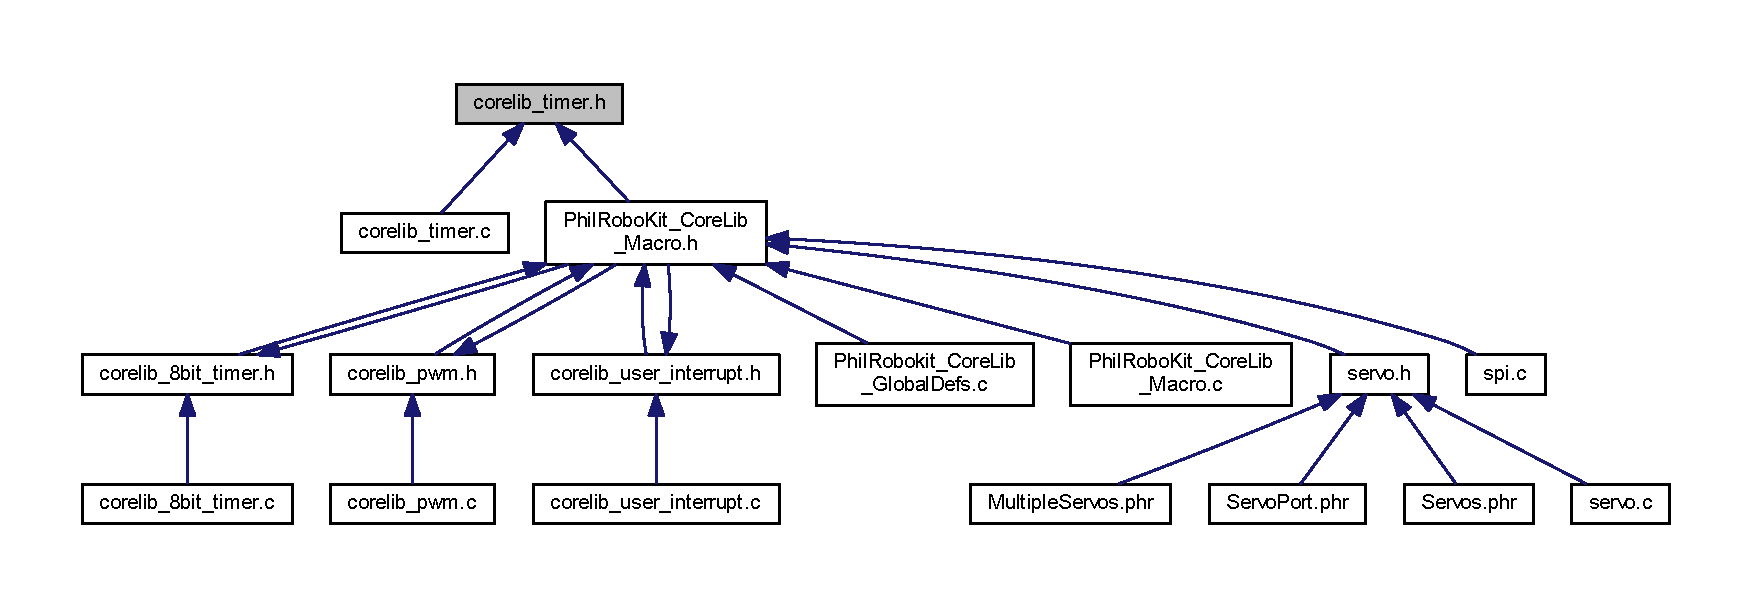
\includegraphics[width=350pt]{corelib__timer_8h__dep__incl}
\end{center}
\end{figure}
\subsection*{Macros}
\begin{DoxyCompactItemize}
\item 
\#define {\bf setup\-Timer}()~{\bf timer\-Init}()
\item 
\#define {\bf C\-O\-N\-S\-T8\-\_\-\-T\-I\-M\-E\-R\-\_\-10\-U\-S}~(65530)
\item 
\#define {\bf C\-O\-N\-S\-T8\-\_\-\-T\-I\-M\-E\-R\-\_\-40\-U\-S}~(65511)
\item 
\#define {\bf C\-O\-N\-S\-T8\-\_\-\-T\-I\-M\-E\-R\-\_\-100\-U\-S}~(65473)
\item 
\#define {\bf C\-O\-N\-S\-T8\-\_\-\-T\-I\-M\-E\-R\-\_\-1000\-U\-S}~(64911)
\item 
\#define {\bf C\-O\-N\-S\-T16\-\_\-\-T\-I\-M\-E\-R}~{\bf C\-O\-N\-S\-T8\-\_\-\-T\-I\-M\-E\-R\-\_\-100\-U\-S}
\item 
\#define {\bf C\-O\-N\-S\-T16\-\_\-\-T\-I\-M\-E\-R\-\_\-\-I\-N\-C\-R\-E\-M\-E\-N\-T}~100
\end{DoxyCompactItemize}
\subsection*{Functions}
\begin{DoxyCompactItemize}
\item 
void {\bf timer\-Interrupt\-Handler} (void)
\item 
void {\bf timer\-Init} (void)
\item 
unsigned int {\bf get\-Elapsed\-Time\-Ms} (unsigned int ui\-Time\-Ms)
\item 
unsigned int {\bf get\-Time\-Ms} (void)
\item 
unsigned int {\bf get\-Elapsed\-Time\-Us} (unsigned int ui\-Time\-Us)
\item 
unsigned int {\bf get\-Time\-Us} (void)
\end{DoxyCompactItemize}


\subsection{Macro Definition Documentation}
\index{corelib\-\_\-timer.\-h@{corelib\-\_\-timer.\-h}!C\-O\-N\-S\-T16\-\_\-\-T\-I\-M\-E\-R@{C\-O\-N\-S\-T16\-\_\-\-T\-I\-M\-E\-R}}
\index{C\-O\-N\-S\-T16\-\_\-\-T\-I\-M\-E\-R@{C\-O\-N\-S\-T16\-\_\-\-T\-I\-M\-E\-R}!corelib_timer.h@{corelib\-\_\-timer.\-h}}
\subsubsection[{C\-O\-N\-S\-T16\-\_\-\-T\-I\-M\-E\-R}]{\setlength{\rightskip}{0pt plus 5cm}\#define C\-O\-N\-S\-T16\-\_\-\-T\-I\-M\-E\-R~{\bf C\-O\-N\-S\-T8\-\_\-\-T\-I\-M\-E\-R\-\_\-100\-U\-S}}\label{corelib__timer_8h_ab1e34d0568170099c396c1c17e32c0f4}


Definition at line 59 of file corelib\-\_\-timer.\-h.

\index{corelib\-\_\-timer.\-h@{corelib\-\_\-timer.\-h}!C\-O\-N\-S\-T16\-\_\-\-T\-I\-M\-E\-R\-\_\-\-I\-N\-C\-R\-E\-M\-E\-N\-T@{C\-O\-N\-S\-T16\-\_\-\-T\-I\-M\-E\-R\-\_\-\-I\-N\-C\-R\-E\-M\-E\-N\-T}}
\index{C\-O\-N\-S\-T16\-\_\-\-T\-I\-M\-E\-R\-\_\-\-I\-N\-C\-R\-E\-M\-E\-N\-T@{C\-O\-N\-S\-T16\-\_\-\-T\-I\-M\-E\-R\-\_\-\-I\-N\-C\-R\-E\-M\-E\-N\-T}!corelib_timer.h@{corelib\-\_\-timer.\-h}}
\subsubsection[{C\-O\-N\-S\-T16\-\_\-\-T\-I\-M\-E\-R\-\_\-\-I\-N\-C\-R\-E\-M\-E\-N\-T}]{\setlength{\rightskip}{0pt plus 5cm}\#define C\-O\-N\-S\-T16\-\_\-\-T\-I\-M\-E\-R\-\_\-\-I\-N\-C\-R\-E\-M\-E\-N\-T~100}\label{corelib__timer_8h_a764ff9c4a8cbf28b27f7183e61532701}


Definition at line 66 of file corelib\-\_\-timer.\-h.

\index{corelib\-\_\-timer.\-h@{corelib\-\_\-timer.\-h}!C\-O\-N\-S\-T8\-\_\-\-T\-I\-M\-E\-R\-\_\-1000\-U\-S@{C\-O\-N\-S\-T8\-\_\-\-T\-I\-M\-E\-R\-\_\-1000\-U\-S}}
\index{C\-O\-N\-S\-T8\-\_\-\-T\-I\-M\-E\-R\-\_\-1000\-U\-S@{C\-O\-N\-S\-T8\-\_\-\-T\-I\-M\-E\-R\-\_\-1000\-U\-S}!corelib_timer.h@{corelib\-\_\-timer.\-h}}
\subsubsection[{C\-O\-N\-S\-T8\-\_\-\-T\-I\-M\-E\-R\-\_\-1000\-U\-S}]{\setlength{\rightskip}{0pt plus 5cm}\#define C\-O\-N\-S\-T8\-\_\-\-T\-I\-M\-E\-R\-\_\-1000\-U\-S~(64911)}\label{corelib__timer_8h_a84acf4a011f9e3ef7f80ed2acc9e8911}


Definition at line 57 of file corelib\-\_\-timer.\-h.

\index{corelib\-\_\-timer.\-h@{corelib\-\_\-timer.\-h}!C\-O\-N\-S\-T8\-\_\-\-T\-I\-M\-E\-R\-\_\-100\-U\-S@{C\-O\-N\-S\-T8\-\_\-\-T\-I\-M\-E\-R\-\_\-100\-U\-S}}
\index{C\-O\-N\-S\-T8\-\_\-\-T\-I\-M\-E\-R\-\_\-100\-U\-S@{C\-O\-N\-S\-T8\-\_\-\-T\-I\-M\-E\-R\-\_\-100\-U\-S}!corelib_timer.h@{corelib\-\_\-timer.\-h}}
\subsubsection[{C\-O\-N\-S\-T8\-\_\-\-T\-I\-M\-E\-R\-\_\-100\-U\-S}]{\setlength{\rightskip}{0pt plus 5cm}\#define C\-O\-N\-S\-T8\-\_\-\-T\-I\-M\-E\-R\-\_\-100\-U\-S~(65473)}\label{corelib__timer_8h_acec7f308afa3fe03929c63cbd7142518}


Definition at line 56 of file corelib\-\_\-timer.\-h.

\index{corelib\-\_\-timer.\-h@{corelib\-\_\-timer.\-h}!C\-O\-N\-S\-T8\-\_\-\-T\-I\-M\-E\-R\-\_\-10\-U\-S@{C\-O\-N\-S\-T8\-\_\-\-T\-I\-M\-E\-R\-\_\-10\-U\-S}}
\index{C\-O\-N\-S\-T8\-\_\-\-T\-I\-M\-E\-R\-\_\-10\-U\-S@{C\-O\-N\-S\-T8\-\_\-\-T\-I\-M\-E\-R\-\_\-10\-U\-S}!corelib_timer.h@{corelib\-\_\-timer.\-h}}
\subsubsection[{C\-O\-N\-S\-T8\-\_\-\-T\-I\-M\-E\-R\-\_\-10\-U\-S}]{\setlength{\rightskip}{0pt plus 5cm}\#define C\-O\-N\-S\-T8\-\_\-\-T\-I\-M\-E\-R\-\_\-10\-U\-S~(65530)}\label{corelib__timer_8h_a7d10b4c09bb287c15fb884bf2c494fb6}


Definition at line 54 of file corelib\-\_\-timer.\-h.

\index{corelib\-\_\-timer.\-h@{corelib\-\_\-timer.\-h}!C\-O\-N\-S\-T8\-\_\-\-T\-I\-M\-E\-R\-\_\-40\-U\-S@{C\-O\-N\-S\-T8\-\_\-\-T\-I\-M\-E\-R\-\_\-40\-U\-S}}
\index{C\-O\-N\-S\-T8\-\_\-\-T\-I\-M\-E\-R\-\_\-40\-U\-S@{C\-O\-N\-S\-T8\-\_\-\-T\-I\-M\-E\-R\-\_\-40\-U\-S}!corelib_timer.h@{corelib\-\_\-timer.\-h}}
\subsubsection[{C\-O\-N\-S\-T8\-\_\-\-T\-I\-M\-E\-R\-\_\-40\-U\-S}]{\setlength{\rightskip}{0pt plus 5cm}\#define C\-O\-N\-S\-T8\-\_\-\-T\-I\-M\-E\-R\-\_\-40\-U\-S~(65511)}\label{corelib__timer_8h_a11f28503310cb1f04502255784f1e75e}


Definition at line 55 of file corelib\-\_\-timer.\-h.

\index{corelib\-\_\-timer.\-h@{corelib\-\_\-timer.\-h}!setup\-Timer@{setup\-Timer}}
\index{setup\-Timer@{setup\-Timer}!corelib_timer.h@{corelib\-\_\-timer.\-h}}
\subsubsection[{setup\-Timer}]{\setlength{\rightskip}{0pt plus 5cm}\#define setup\-Timer(
\begin{DoxyParamCaption}
{}
\end{DoxyParamCaption}
)~{\bf timer\-Init}()}\label{corelib__timer_8h_aaf8f8cfbfa3cd87d92855860610e801f}


Definition at line 52 of file corelib\-\_\-timer.\-h.



\subsection{Function Documentation}
\index{corelib\-\_\-timer.\-h@{corelib\-\_\-timer.\-h}!get\-Elapsed\-Time\-Ms@{get\-Elapsed\-Time\-Ms}}
\index{get\-Elapsed\-Time\-Ms@{get\-Elapsed\-Time\-Ms}!corelib_timer.h@{corelib\-\_\-timer.\-h}}
\subsubsection[{get\-Elapsed\-Time\-Ms}]{\setlength{\rightskip}{0pt plus 5cm}unsigned int get\-Elapsed\-Time\-Ms (
\begin{DoxyParamCaption}
\item[{unsigned int}]{ui\-Time\-Ms}
\end{DoxyParamCaption}
)}\label{corelib__timer_8h_acf72cf4216df47fd55b2b68944acd8e7}


Definition at line 83 of file corelib\-\_\-timer.\-c.

\index{corelib\-\_\-timer.\-h@{corelib\-\_\-timer.\-h}!get\-Elapsed\-Time\-Us@{get\-Elapsed\-Time\-Us}}
\index{get\-Elapsed\-Time\-Us@{get\-Elapsed\-Time\-Us}!corelib_timer.h@{corelib\-\_\-timer.\-h}}
\subsubsection[{get\-Elapsed\-Time\-Us}]{\setlength{\rightskip}{0pt plus 5cm}unsigned int get\-Elapsed\-Time\-Us (
\begin{DoxyParamCaption}
\item[{unsigned int}]{ui\-Time\-Us}
\end{DoxyParamCaption}
)}\label{corelib__timer_8h_a0493c088a76d2d3ab4037d3f8ddcdb96}


Definition at line 93 of file corelib\-\_\-timer.\-c.

\index{corelib\-\_\-timer.\-h@{corelib\-\_\-timer.\-h}!get\-Time\-Ms@{get\-Time\-Ms}}
\index{get\-Time\-Ms@{get\-Time\-Ms}!corelib_timer.h@{corelib\-\_\-timer.\-h}}
\subsubsection[{get\-Time\-Ms}]{\setlength{\rightskip}{0pt plus 5cm}unsigned int get\-Time\-Ms (
\begin{DoxyParamCaption}
\item[{void}]{}
\end{DoxyParamCaption}
)}\label{corelib__timer_8h_ae9bfb9f90b70aa56cee9f098bc432af9}


Definition at line 88 of file corelib\-\_\-timer.\-c.

\index{corelib\-\_\-timer.\-h@{corelib\-\_\-timer.\-h}!get\-Time\-Us@{get\-Time\-Us}}
\index{get\-Time\-Us@{get\-Time\-Us}!corelib_timer.h@{corelib\-\_\-timer.\-h}}
\subsubsection[{get\-Time\-Us}]{\setlength{\rightskip}{0pt plus 5cm}unsigned int get\-Time\-Us (
\begin{DoxyParamCaption}
\item[{void}]{}
\end{DoxyParamCaption}
)}\label{corelib__timer_8h_a266203d02833370efae4349490a6046f}


Definition at line 98 of file corelib\-\_\-timer.\-c.

\index{corelib\-\_\-timer.\-h@{corelib\-\_\-timer.\-h}!timer\-Init@{timer\-Init}}
\index{timer\-Init@{timer\-Init}!corelib_timer.h@{corelib\-\_\-timer.\-h}}
\subsubsection[{timer\-Init}]{\setlength{\rightskip}{0pt plus 5cm}void timer\-Init (
\begin{DoxyParamCaption}
\item[{void}]{}
\end{DoxyParamCaption}
)}\label{corelib__timer_8h_a1cabbdb02f36420b24c4ccd132972080}


Definition at line 63 of file corelib\-\_\-timer.\-c.

\index{corelib\-\_\-timer.\-h@{corelib\-\_\-timer.\-h}!timer\-Interrupt\-Handler@{timer\-Interrupt\-Handler}}
\index{timer\-Interrupt\-Handler@{timer\-Interrupt\-Handler}!corelib_timer.h@{corelib\-\_\-timer.\-h}}
\subsubsection[{timer\-Interrupt\-Handler}]{\setlength{\rightskip}{0pt plus 5cm}void timer\-Interrupt\-Handler (
\begin{DoxyParamCaption}
\item[{void}]{}
\end{DoxyParamCaption}
)}\label{corelib__timer_8h_ae6b9991ee92a30ad115ef6928829566a}


Definition at line 39 of file corelib\-\_\-timer.\-c.


\section{corelib\-\_\-uart.\-c File Reference}
\label{corelib__uart_8c}\index{corelib\-\_\-uart.\-c@{corelib\-\_\-uart.\-c}}
{\ttfamily \#include \char`\"{}corelib\-\_\-uart.\-h\char`\"{}}\\*
{\ttfamily \#include \char`\"{}string.\-h\char`\"{}}\\*
Include dependency graph for corelib\-\_\-uart.\-c\-:\nopagebreak
\begin{figure}[H]
\begin{center}
\leavevmode
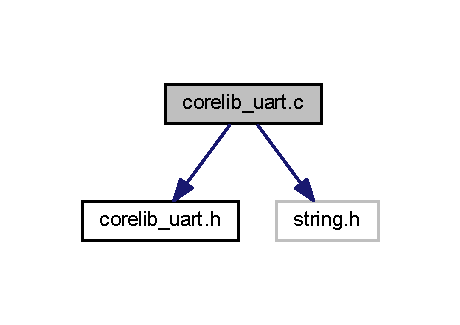
\includegraphics[width=221pt]{corelib__uart_8c__incl}
\end{center}
\end{figure}
\subsection*{Functions}
\begin{DoxyCompactItemize}
\item 
void {\bf setup\-Serial} (unsigned int i\-Baudrate)
\item 
unsigned char {\bf is\-Serial\-Buffer\-Full} (void)
\item 
void {\bf serial\-Send\-Char} (unsigned char uc\-Tx\-Data)
\item 
void {\bf serial\-Send\-String} (unsigned char $\ast$uc\-Str\-Tx\-Data)
\item 
unsigned char {\bf is\-Serial\-Data\-Available} (void)
\item 
unsigned char {\bf serial\-Read} (void)
\item 
void {\bf serial\-Flush\-Data} (void)
\item 
void {\bf serial\-Rx\-Interrupt\-Handler} (void)
\item 
void {\bf serial\-Tx\-Interrupt\-Handler} (void)
\end{DoxyCompactItemize}


\subsection{Function Documentation}
\index{corelib\-\_\-uart.\-c@{corelib\-\_\-uart.\-c}!is\-Serial\-Buffer\-Full@{is\-Serial\-Buffer\-Full}}
\index{is\-Serial\-Buffer\-Full@{is\-Serial\-Buffer\-Full}!corelib_uart.c@{corelib\-\_\-uart.\-c}}
\subsubsection[{is\-Serial\-Buffer\-Full}]{\setlength{\rightskip}{0pt plus 5cm}unsigned char is\-Serial\-Buffer\-Full (
\begin{DoxyParamCaption}
\item[{void}]{}
\end{DoxyParamCaption}
)}\label{corelib__uart_8c_acbd06afbb8c5228e13793b78aff16055}


Definition at line 91 of file corelib\-\_\-uart.\-c.

\index{corelib\-\_\-uart.\-c@{corelib\-\_\-uart.\-c}!is\-Serial\-Data\-Available@{is\-Serial\-Data\-Available}}
\index{is\-Serial\-Data\-Available@{is\-Serial\-Data\-Available}!corelib_uart.c@{corelib\-\_\-uart.\-c}}
\subsubsection[{is\-Serial\-Data\-Available}]{\setlength{\rightskip}{0pt plus 5cm}unsigned char is\-Serial\-Data\-Available (
\begin{DoxyParamCaption}
\item[{void}]{}
\end{DoxyParamCaption}
)}\label{corelib__uart_8c_a658378a2f5a1d0f9d2b1e914342274ba}


Definition at line 119 of file corelib\-\_\-uart.\-c.

\index{corelib\-\_\-uart.\-c@{corelib\-\_\-uart.\-c}!serial\-Flush\-Data@{serial\-Flush\-Data}}
\index{serial\-Flush\-Data@{serial\-Flush\-Data}!corelib_uart.c@{corelib\-\_\-uart.\-c}}
\subsubsection[{serial\-Flush\-Data}]{\setlength{\rightskip}{0pt plus 5cm}void serial\-Flush\-Data (
\begin{DoxyParamCaption}
\item[{void}]{}
\end{DoxyParamCaption}
)}\label{corelib__uart_8c_aa1e1f13e87f29d62164aff7384a886d7}


Definition at line 154 of file corelib\-\_\-uart.\-c.

\index{corelib\-\_\-uart.\-c@{corelib\-\_\-uart.\-c}!serial\-Read@{serial\-Read}}
\index{serial\-Read@{serial\-Read}!corelib_uart.c@{corelib\-\_\-uart.\-c}}
\subsubsection[{serial\-Read}]{\setlength{\rightskip}{0pt plus 5cm}unsigned char serial\-Read (
\begin{DoxyParamCaption}
\item[{void}]{}
\end{DoxyParamCaption}
)}\label{corelib__uart_8c_a02ecb039425503e2981f491fe7c85cf7}


Definition at line 131 of file corelib\-\_\-uart.\-c.



Here is the call graph for this function\-:\nopagebreak
\begin{figure}[H]
\begin{center}
\leavevmode
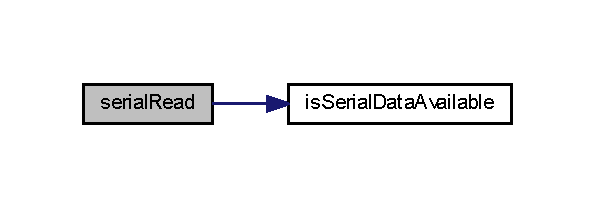
\includegraphics[width=286pt]{corelib__uart_8c_a02ecb039425503e2981f491fe7c85cf7_cgraph}
\end{center}
\end{figure}


\index{corelib\-\_\-uart.\-c@{corelib\-\_\-uart.\-c}!serial\-Rx\-Interrupt\-Handler@{serial\-Rx\-Interrupt\-Handler}}
\index{serial\-Rx\-Interrupt\-Handler@{serial\-Rx\-Interrupt\-Handler}!corelib_uart.c@{corelib\-\_\-uart.\-c}}
\subsubsection[{serial\-Rx\-Interrupt\-Handler}]{\setlength{\rightskip}{0pt plus 5cm}void serial\-Rx\-Interrupt\-Handler (
\begin{DoxyParamCaption}
\item[{void}]{}
\end{DoxyParamCaption}
)}\label{corelib__uart_8c_ae0717c2e8facfb4304da7e22d0127310}


Definition at line 165 of file corelib\-\_\-uart.\-c.

\index{corelib\-\_\-uart.\-c@{corelib\-\_\-uart.\-c}!serial\-Send\-Char@{serial\-Send\-Char}}
\index{serial\-Send\-Char@{serial\-Send\-Char}!corelib_uart.c@{corelib\-\_\-uart.\-c}}
\subsubsection[{serial\-Send\-Char}]{\setlength{\rightskip}{0pt plus 5cm}void serial\-Send\-Char (
\begin{DoxyParamCaption}
\item[{unsigned char}]{uc\-Tx\-Data}
\end{DoxyParamCaption}
)}\label{corelib__uart_8c_a6c415891a7120c91d1e8f02d47f7c366}


Definition at line 96 of file corelib\-\_\-uart.\-c.



Here is the call graph for this function\-:\nopagebreak
\begin{figure}[H]
\begin{center}
\leavevmode
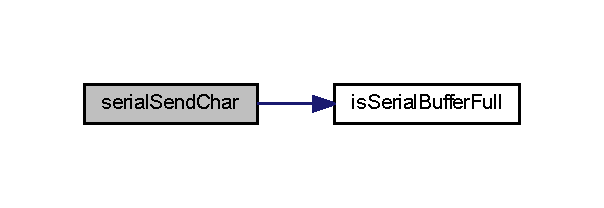
\includegraphics[width=290pt]{corelib__uart_8c_a6c415891a7120c91d1e8f02d47f7c366_cgraph}
\end{center}
\end{figure}


\index{corelib\-\_\-uart.\-c@{corelib\-\_\-uart.\-c}!serial\-Send\-String@{serial\-Send\-String}}
\index{serial\-Send\-String@{serial\-Send\-String}!corelib_uart.c@{corelib\-\_\-uart.\-c}}
\subsubsection[{serial\-Send\-String}]{\setlength{\rightskip}{0pt plus 5cm}void serial\-Send\-String (
\begin{DoxyParamCaption}
\item[{unsigned char $\ast$}]{uc\-Str\-Tx\-Data}
\end{DoxyParamCaption}
)}\label{corelib__uart_8c_aaaf3b133fc1a7ea81b05ff0786c96765}


Definition at line 112 of file corelib\-\_\-uart.\-c.



Here is the call graph for this function\-:\nopagebreak
\begin{figure}[H]
\begin{center}
\leavevmode
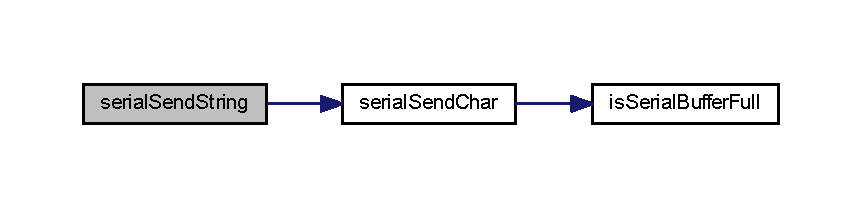
\includegraphics[width=350pt]{corelib__uart_8c_aaaf3b133fc1a7ea81b05ff0786c96765_cgraph}
\end{center}
\end{figure}


\index{corelib\-\_\-uart.\-c@{corelib\-\_\-uart.\-c}!serial\-Tx\-Interrupt\-Handler@{serial\-Tx\-Interrupt\-Handler}}
\index{serial\-Tx\-Interrupt\-Handler@{serial\-Tx\-Interrupt\-Handler}!corelib_uart.c@{corelib\-\_\-uart.\-c}}
\subsubsection[{serial\-Tx\-Interrupt\-Handler}]{\setlength{\rightskip}{0pt plus 5cm}void serial\-Tx\-Interrupt\-Handler (
\begin{DoxyParamCaption}
\item[{void}]{}
\end{DoxyParamCaption}
)}\label{corelib__uart_8c_a6e374afdfd344351c59c2005a0b1eee0}


Definition at line 181 of file corelib\-\_\-uart.\-c.

\index{corelib\-\_\-uart.\-c@{corelib\-\_\-uart.\-c}!setup\-Serial@{setup\-Serial}}
\index{setup\-Serial@{setup\-Serial}!corelib_uart.c@{corelib\-\_\-uart.\-c}}
\subsubsection[{setup\-Serial}]{\setlength{\rightskip}{0pt plus 5cm}void setup\-Serial (
\begin{DoxyParamCaption}
\item[{unsigned int}]{i\-Baudrate}
\end{DoxyParamCaption}
)}\label{corelib__uart_8c_a1854f41b5e5e42677e9d3f85f28f64a5}


Definition at line 34 of file corelib\-\_\-uart.\-c.


\section{corelib\-\_\-uart.\-h File Reference}
\label{corelib__uart_8h}\index{corelib\-\_\-uart.\-h@{corelib\-\_\-uart.\-h}}
This graph shows which files directly or indirectly include this file\-:\nopagebreak
\begin{figure}[H]
\begin{center}
\leavevmode
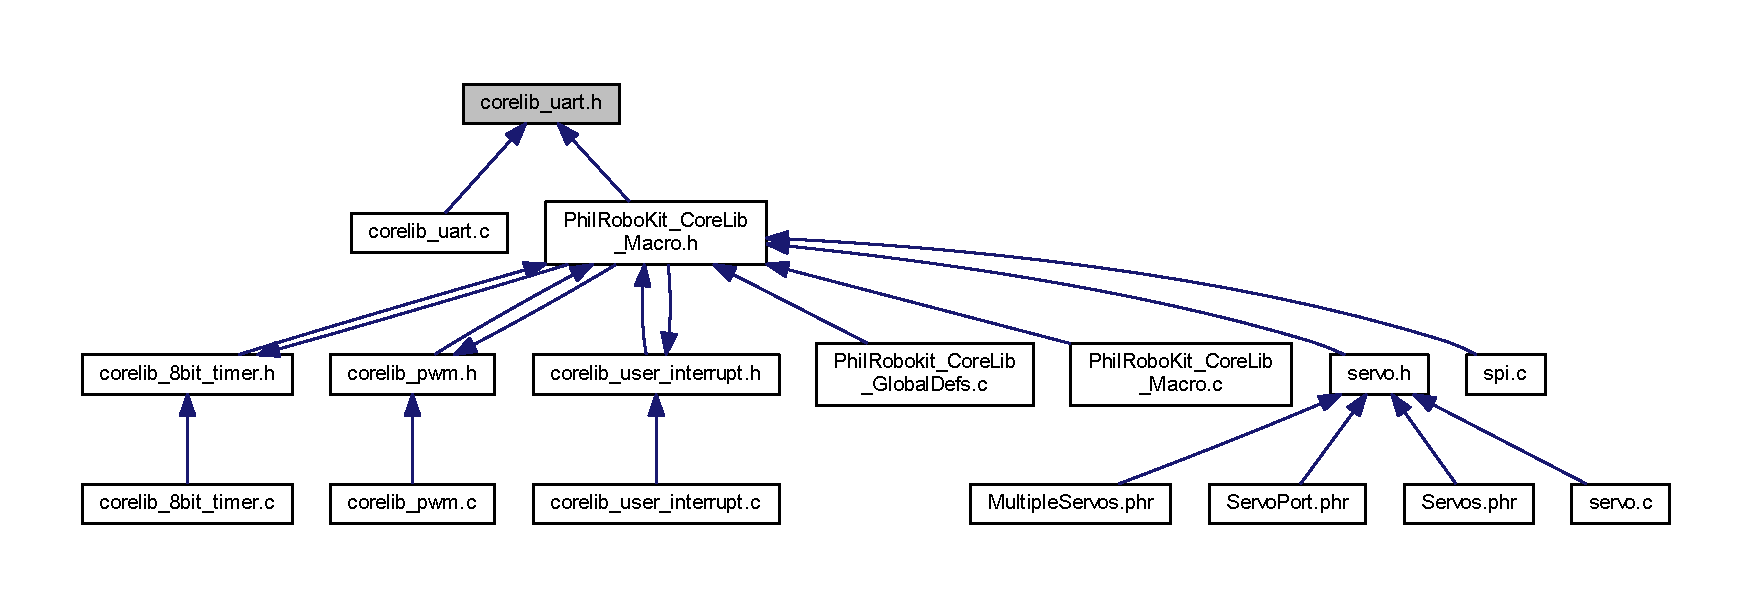
\includegraphics[width=350pt]{corelib__uart_8h__dep__incl}
\end{center}
\end{figure}
\subsection*{Macros}
\begin{DoxyCompactItemize}
\item 
\#define {\bf N\-U\-L\-L}~'\textbackslash{}0'
\item 
\#define {\bf B\-A\-U\-D\-R\-A\-T\-E}(x)~((20000000 /$\ast$ui\-Freq\-O\-S\-C$\ast$/ / x)/16) -\/1
\item 
\#define {\bf B\-U\-F\-F\-E\-R\-\_\-\-S\-I\-Z\-E}~16
\end{DoxyCompactItemize}
\subsection*{Functions}
\begin{DoxyCompactItemize}
\item 
void {\bf setup\-Serial} (unsigned int i\-Baudrate)
\item 
void {\bf serial\-Send\-Char} (unsigned char uc\-Tx\-Data)
\item 
void {\bf serial\-Send\-String} (unsigned char $\ast$uc\-Str\-Tx\-Data)
\item 
unsigned char {\bf serial\-Read} (void)
\item 
unsigned char {\bf is\-Serial\-Data\-Available} (void)
\item 
void {\bf serial\-Flush\-Data} (void)
\item 
void {\bf serial\-Rx\-Interrupt\-Handler} (void)
\item 
void {\bf serial\-Tx\-Interrupt\-Handler} (void)
\end{DoxyCompactItemize}
\subsection*{Variables}
\begin{DoxyCompactItemize}
\item 
\begin{tabbing}
xx\=xx\=xx\=xx\=xx\=xx\=xx\=xx\=xx\=\kill
struct \{\\
\>unsigned char {\bf ucBuffer} [{\bf BUFFER\_SIZE}]\\
\>unsigned int {\bf iIn}\\
\>unsigned int {\bf iOut}\\
\} {\bf TXFiFo}\\

\end{tabbing}\item 
\begin{tabbing}
xx\=xx\=xx\=xx\=xx\=xx\=xx\=xx\=xx\=\kill
struct \{\\
\>unsigned char {\bf ucBuffer} [{\bf BUFFER\_SIZE}]\\
\>unsigned int {\bf iIn}\\
\>unsigned int {\bf iOut}\\
\} {\bf RXFiFo}\\

\end{tabbing}\end{DoxyCompactItemize}


\subsection{Macro Definition Documentation}
\index{corelib\-\_\-uart.\-h@{corelib\-\_\-uart.\-h}!B\-A\-U\-D\-R\-A\-T\-E@{B\-A\-U\-D\-R\-A\-T\-E}}
\index{B\-A\-U\-D\-R\-A\-T\-E@{B\-A\-U\-D\-R\-A\-T\-E}!corelib_uart.h@{corelib\-\_\-uart.\-h}}
\subsubsection[{B\-A\-U\-D\-R\-A\-T\-E}]{\setlength{\rightskip}{0pt plus 5cm}\#define B\-A\-U\-D\-R\-A\-T\-E(
\begin{DoxyParamCaption}
\item[{}]{x}
\end{DoxyParamCaption}
)~((20000000 /$\ast$ui\-Freq\-O\-S\-C$\ast$/ / x)/16) -\/1}\label{corelib__uart_8h_ad1d695497aaa25bf1de5c76b7222713c}


Definition at line 71 of file corelib\-\_\-uart.\-h.

\index{corelib\-\_\-uart.\-h@{corelib\-\_\-uart.\-h}!B\-U\-F\-F\-E\-R\-\_\-\-S\-I\-Z\-E@{B\-U\-F\-F\-E\-R\-\_\-\-S\-I\-Z\-E}}
\index{B\-U\-F\-F\-E\-R\-\_\-\-S\-I\-Z\-E@{B\-U\-F\-F\-E\-R\-\_\-\-S\-I\-Z\-E}!corelib_uart.h@{corelib\-\_\-uart.\-h}}
\subsubsection[{B\-U\-F\-F\-E\-R\-\_\-\-S\-I\-Z\-E}]{\setlength{\rightskip}{0pt plus 5cm}\#define B\-U\-F\-F\-E\-R\-\_\-\-S\-I\-Z\-E~16}\label{corelib__uart_8h_a6b20d41d6252e9871430c242cb1a56e7}


Definition at line 72 of file corelib\-\_\-uart.\-h.

\index{corelib\-\_\-uart.\-h@{corelib\-\_\-uart.\-h}!N\-U\-L\-L@{N\-U\-L\-L}}
\index{N\-U\-L\-L@{N\-U\-L\-L}!corelib_uart.h@{corelib\-\_\-uart.\-h}}
\subsubsection[{N\-U\-L\-L}]{\setlength{\rightskip}{0pt plus 5cm}\#define N\-U\-L\-L~'\textbackslash{}0'}\label{corelib__uart_8h_a070d2ce7b6bb7e5c05602aa8c308d0c4}


Definition at line 52 of file corelib\-\_\-uart.\-h.



\subsection{Function Documentation}
\index{corelib\-\_\-uart.\-h@{corelib\-\_\-uart.\-h}!is\-Serial\-Data\-Available@{is\-Serial\-Data\-Available}}
\index{is\-Serial\-Data\-Available@{is\-Serial\-Data\-Available}!corelib_uart.h@{corelib\-\_\-uart.\-h}}
\subsubsection[{is\-Serial\-Data\-Available}]{\setlength{\rightskip}{0pt plus 5cm}unsigned char is\-Serial\-Data\-Available (
\begin{DoxyParamCaption}
\item[{void}]{}
\end{DoxyParamCaption}
)}\label{corelib__uart_8h_a658378a2f5a1d0f9d2b1e914342274ba}


Definition at line 119 of file corelib\-\_\-uart.\-c.

\index{corelib\-\_\-uart.\-h@{corelib\-\_\-uart.\-h}!serial\-Flush\-Data@{serial\-Flush\-Data}}
\index{serial\-Flush\-Data@{serial\-Flush\-Data}!corelib_uart.h@{corelib\-\_\-uart.\-h}}
\subsubsection[{serial\-Flush\-Data}]{\setlength{\rightskip}{0pt plus 5cm}void serial\-Flush\-Data (
\begin{DoxyParamCaption}
\item[{void}]{}
\end{DoxyParamCaption}
)}\label{corelib__uart_8h_aa1e1f13e87f29d62164aff7384a886d7}


Definition at line 154 of file corelib\-\_\-uart.\-c.

\index{corelib\-\_\-uart.\-h@{corelib\-\_\-uart.\-h}!serial\-Read@{serial\-Read}}
\index{serial\-Read@{serial\-Read}!corelib_uart.h@{corelib\-\_\-uart.\-h}}
\subsubsection[{serial\-Read}]{\setlength{\rightskip}{0pt plus 5cm}unsigned char serial\-Read (
\begin{DoxyParamCaption}
\item[{void}]{}
\end{DoxyParamCaption}
)}\label{corelib__uart_8h_a02ecb039425503e2981f491fe7c85cf7}


Definition at line 131 of file corelib\-\_\-uart.\-c.



Here is the call graph for this function\-:\nopagebreak
\begin{figure}[H]
\begin{center}
\leavevmode
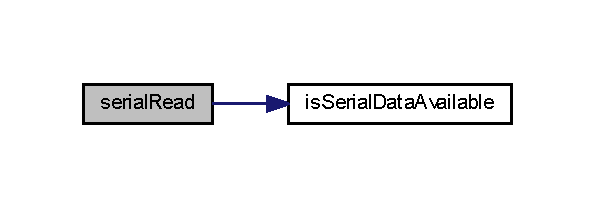
\includegraphics[width=286pt]{corelib__uart_8h_a02ecb039425503e2981f491fe7c85cf7_cgraph}
\end{center}
\end{figure}


\index{corelib\-\_\-uart.\-h@{corelib\-\_\-uart.\-h}!serial\-Rx\-Interrupt\-Handler@{serial\-Rx\-Interrupt\-Handler}}
\index{serial\-Rx\-Interrupt\-Handler@{serial\-Rx\-Interrupt\-Handler}!corelib_uart.h@{corelib\-\_\-uart.\-h}}
\subsubsection[{serial\-Rx\-Interrupt\-Handler}]{\setlength{\rightskip}{0pt plus 5cm}void serial\-Rx\-Interrupt\-Handler (
\begin{DoxyParamCaption}
\item[{void}]{}
\end{DoxyParamCaption}
)}\label{corelib__uart_8h_ae0717c2e8facfb4304da7e22d0127310}


Definition at line 165 of file corelib\-\_\-uart.\-c.

\index{corelib\-\_\-uart.\-h@{corelib\-\_\-uart.\-h}!serial\-Send\-Char@{serial\-Send\-Char}}
\index{serial\-Send\-Char@{serial\-Send\-Char}!corelib_uart.h@{corelib\-\_\-uart.\-h}}
\subsubsection[{serial\-Send\-Char}]{\setlength{\rightskip}{0pt plus 5cm}void serial\-Send\-Char (
\begin{DoxyParamCaption}
\item[{unsigned char}]{uc\-Tx\-Data}
\end{DoxyParamCaption}
)}\label{corelib__uart_8h_a6c415891a7120c91d1e8f02d47f7c366}


Definition at line 96 of file corelib\-\_\-uart.\-c.



Here is the call graph for this function\-:\nopagebreak
\begin{figure}[H]
\begin{center}
\leavevmode
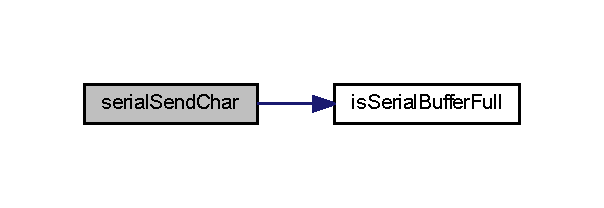
\includegraphics[width=290pt]{corelib__uart_8h_a6c415891a7120c91d1e8f02d47f7c366_cgraph}
\end{center}
\end{figure}


\index{corelib\-\_\-uart.\-h@{corelib\-\_\-uart.\-h}!serial\-Send\-String@{serial\-Send\-String}}
\index{serial\-Send\-String@{serial\-Send\-String}!corelib_uart.h@{corelib\-\_\-uart.\-h}}
\subsubsection[{serial\-Send\-String}]{\setlength{\rightskip}{0pt plus 5cm}void serial\-Send\-String (
\begin{DoxyParamCaption}
\item[{unsigned char $\ast$}]{uc\-Str\-Tx\-Data}
\end{DoxyParamCaption}
)}\label{corelib__uart_8h_aaaf3b133fc1a7ea81b05ff0786c96765}


Definition at line 112 of file corelib\-\_\-uart.\-c.



Here is the call graph for this function\-:\nopagebreak
\begin{figure}[H]
\begin{center}
\leavevmode
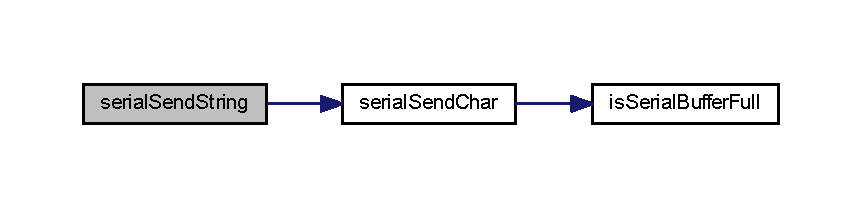
\includegraphics[width=350pt]{corelib__uart_8h_aaaf3b133fc1a7ea81b05ff0786c96765_cgraph}
\end{center}
\end{figure}


\index{corelib\-\_\-uart.\-h@{corelib\-\_\-uart.\-h}!serial\-Tx\-Interrupt\-Handler@{serial\-Tx\-Interrupt\-Handler}}
\index{serial\-Tx\-Interrupt\-Handler@{serial\-Tx\-Interrupt\-Handler}!corelib_uart.h@{corelib\-\_\-uart.\-h}}
\subsubsection[{serial\-Tx\-Interrupt\-Handler}]{\setlength{\rightskip}{0pt plus 5cm}void serial\-Tx\-Interrupt\-Handler (
\begin{DoxyParamCaption}
\item[{void}]{}
\end{DoxyParamCaption}
)}\label{corelib__uart_8h_a6e374afdfd344351c59c2005a0b1eee0}


Definition at line 181 of file corelib\-\_\-uart.\-c.

\index{corelib\-\_\-uart.\-h@{corelib\-\_\-uart.\-h}!setup\-Serial@{setup\-Serial}}
\index{setup\-Serial@{setup\-Serial}!corelib_uart.h@{corelib\-\_\-uart.\-h}}
\subsubsection[{setup\-Serial}]{\setlength{\rightskip}{0pt plus 5cm}void setup\-Serial (
\begin{DoxyParamCaption}
\item[{unsigned int}]{i\-Baudrate}
\end{DoxyParamCaption}
)}\label{corelib__uart_8h_a1854f41b5e5e42677e9d3f85f28f64a5}


Definition at line 34 of file corelib\-\_\-uart.\-c.



\subsection{Variable Documentation}
\index{corelib\-\_\-uart.\-h@{corelib\-\_\-uart.\-h}!i\-In@{i\-In}}
\index{i\-In@{i\-In}!corelib_uart.h@{corelib\-\_\-uart.\-h}}
\subsubsection[{i\-In}]{\setlength{\rightskip}{0pt plus 5cm}unsigned int i\-In}\label{corelib__uart_8h_aa439df2901a799690275b0c20fc85c8f}


Definition at line 76 of file corelib\-\_\-uart.\-h.

\index{corelib\-\_\-uart.\-h@{corelib\-\_\-uart.\-h}!i\-Out@{i\-Out}}
\index{i\-Out@{i\-Out}!corelib_uart.h@{corelib\-\_\-uart.\-h}}
\subsubsection[{i\-Out}]{\setlength{\rightskip}{0pt plus 5cm}unsigned int i\-Out}\label{corelib__uart_8h_a2099e8bfe004ae2e2e0e5dcbc5ff7a75}


Definition at line 77 of file corelib\-\_\-uart.\-h.

\index{corelib\-\_\-uart.\-h@{corelib\-\_\-uart.\-h}!R\-X\-Fi\-Fo@{R\-X\-Fi\-Fo}}
\index{R\-X\-Fi\-Fo@{R\-X\-Fi\-Fo}!corelib_uart.h@{corelib\-\_\-uart.\-h}}
\subsubsection[{R\-X\-Fi\-Fo}]{\setlength{\rightskip}{0pt plus 5cm}struct \{ ... \}   R\-X\-Fi\-Fo}\label{corelib__uart_8h_ac3c8fda82266ec9e5fba3b1285831e42}
\index{corelib\-\_\-uart.\-h@{corelib\-\_\-uart.\-h}!T\-X\-Fi\-Fo@{T\-X\-Fi\-Fo}}
\index{T\-X\-Fi\-Fo@{T\-X\-Fi\-Fo}!corelib_uart.h@{corelib\-\_\-uart.\-h}}
\subsubsection[{T\-X\-Fi\-Fo}]{\setlength{\rightskip}{0pt plus 5cm}struct \{ ... \}  T\-X\-Fi\-Fo}\label{corelib__uart_8h_a13e4e4e6c8e63567fb59f1b2ad920c64}
\index{corelib\-\_\-uart.\-h@{corelib\-\_\-uart.\-h}!uc\-Buffer@{uc\-Buffer}}
\index{uc\-Buffer@{uc\-Buffer}!corelib_uart.h@{corelib\-\_\-uart.\-h}}
\subsubsection[{uc\-Buffer}]{\setlength{\rightskip}{0pt plus 5cm}unsigned char uc\-Buffer[{\bf B\-U\-F\-F\-E\-R\-\_\-\-S\-I\-Z\-E}]}\label{corelib__uart_8h_a2e2f12c2d2723f15fa34d754c9cd8324}


Definition at line 75 of file corelib\-\_\-uart.\-h.


\section{corelib\-\_\-user\-\_\-interrupt.\-c File Reference}
\label{corelib__user__interrupt_8c}\index{corelib\-\_\-user\-\_\-interrupt.\-c@{corelib\-\_\-user\-\_\-interrupt.\-c}}
{\ttfamily \#include \char`\"{}corelib\-\_\-user\-\_\-interrupt.\-h\char`\"{}}\\*
Include dependency graph for corelib\-\_\-user\-\_\-interrupt.\-c\-:\nopagebreak
\begin{figure}[H]
\begin{center}
\leavevmode
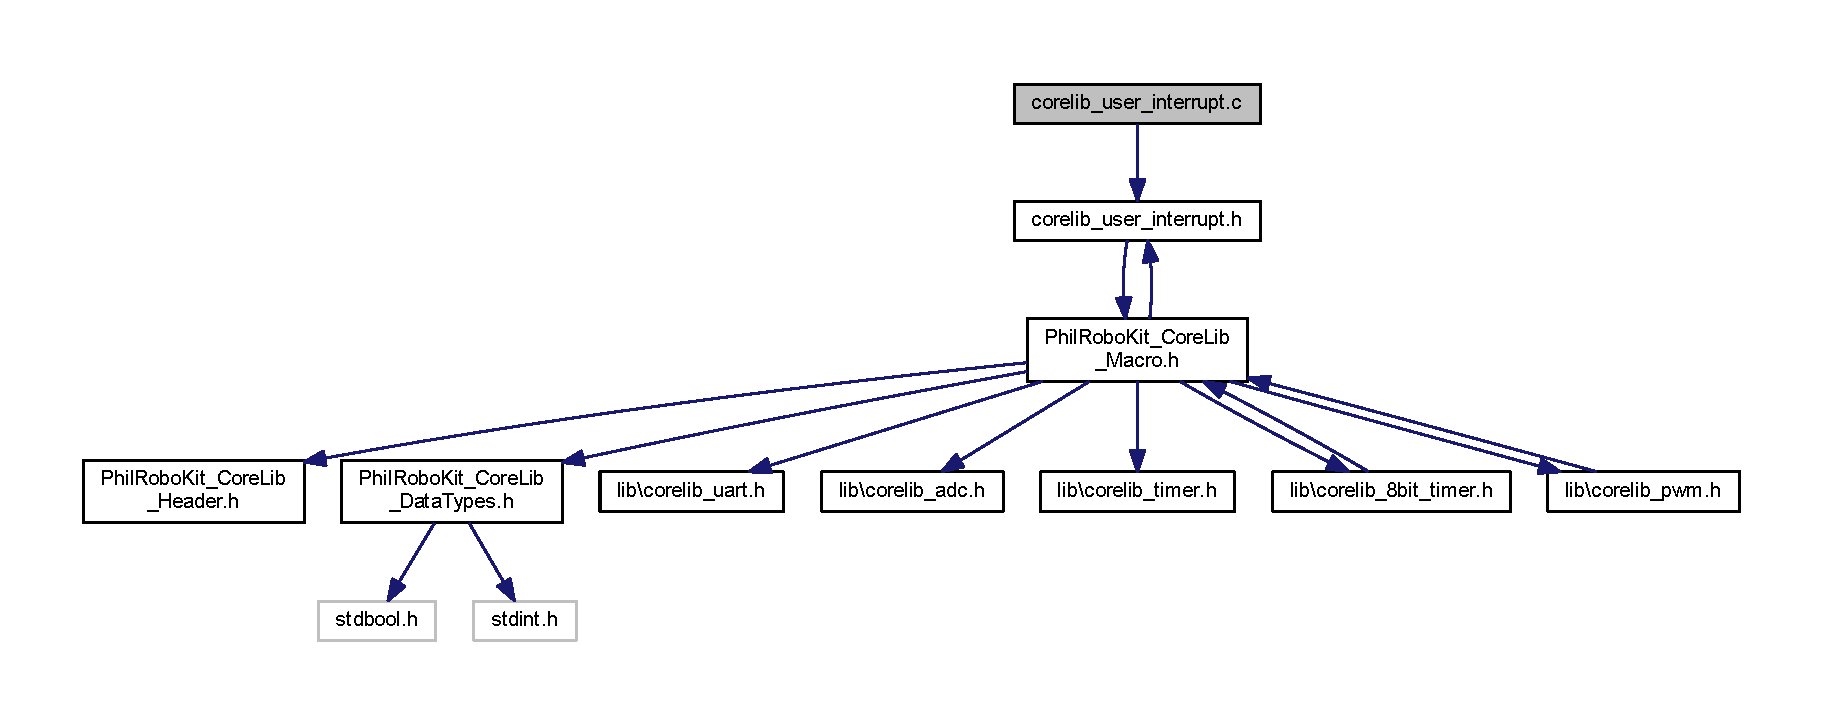
\includegraphics[width=350pt]{corelib__user__interrupt_8c__incl}
\end{center}
\end{figure}
\subsection*{Functions}
\begin{DoxyCompactItemize}
\item 
void {\bf setup\-User\-Interrupt} (enum {\bf et\-Interrupt\-Sources} e\-Int\-Source, void($\ast$function)(), enum {\bf et\-Interrupt\-Modes} e\-Int\-Mode)
\item 
void {\bf user\-Interrupt\-Handler} (void)
\end{DoxyCompactItemize}


\subsection{Function Documentation}
\index{corelib\-\_\-user\-\_\-interrupt.\-c@{corelib\-\_\-user\-\_\-interrupt.\-c}!setup\-User\-Interrupt@{setup\-User\-Interrupt}}
\index{setup\-User\-Interrupt@{setup\-User\-Interrupt}!corelib_user_interrupt.c@{corelib\-\_\-user\-\_\-interrupt.\-c}}
\subsubsection[{setup\-User\-Interrupt}]{\setlength{\rightskip}{0pt plus 5cm}void setup\-User\-Interrupt (
\begin{DoxyParamCaption}
\item[{enum {\bf et\-Interrupt\-Sources}}]{e\-Int\-Source, }
\item[{void($\ast$)()}]{function, }
\item[{enum {\bf et\-Interrupt\-Modes}}]{e\-Int\-Mode}
\end{DoxyParamCaption}
)}\label{corelib__user__interrupt_8c_a234efbd3a1dc891dbfbcd0364a9b52ec}


Definition at line 82 of file corelib\-\_\-user\-\_\-interrupt.\-c.

\index{corelib\-\_\-user\-\_\-interrupt.\-c@{corelib\-\_\-user\-\_\-interrupt.\-c}!user\-Interrupt\-Handler@{user\-Interrupt\-Handler}}
\index{user\-Interrupt\-Handler@{user\-Interrupt\-Handler}!corelib_user_interrupt.c@{corelib\-\_\-user\-\_\-interrupt.\-c}}
\subsubsection[{user\-Interrupt\-Handler}]{\setlength{\rightskip}{0pt plus 5cm}void user\-Interrupt\-Handler (
\begin{DoxyParamCaption}
\item[{void}]{}
\end{DoxyParamCaption}
)}\label{corelib__user__interrupt_8c_aa1ef5be24251d01808e5dec4c6babd01}


Definition at line 178 of file corelib\-\_\-user\-\_\-interrupt.\-c.


\section{corelib\-\_\-user\-\_\-interrupt.\-h File Reference}
\label{corelib__user__interrupt_8h}\index{corelib\-\_\-user\-\_\-interrupt.\-h@{corelib\-\_\-user\-\_\-interrupt.\-h}}
{\ttfamily \#include $<$Phil\-Robo\-Kit\-\_\-\-Core\-Lib\-\_\-\-Macro.\-h$>$}\\*
Include dependency graph for corelib\-\_\-user\-\_\-interrupt.\-h\-:\nopagebreak
\begin{figure}[H]
\begin{center}
\leavevmode
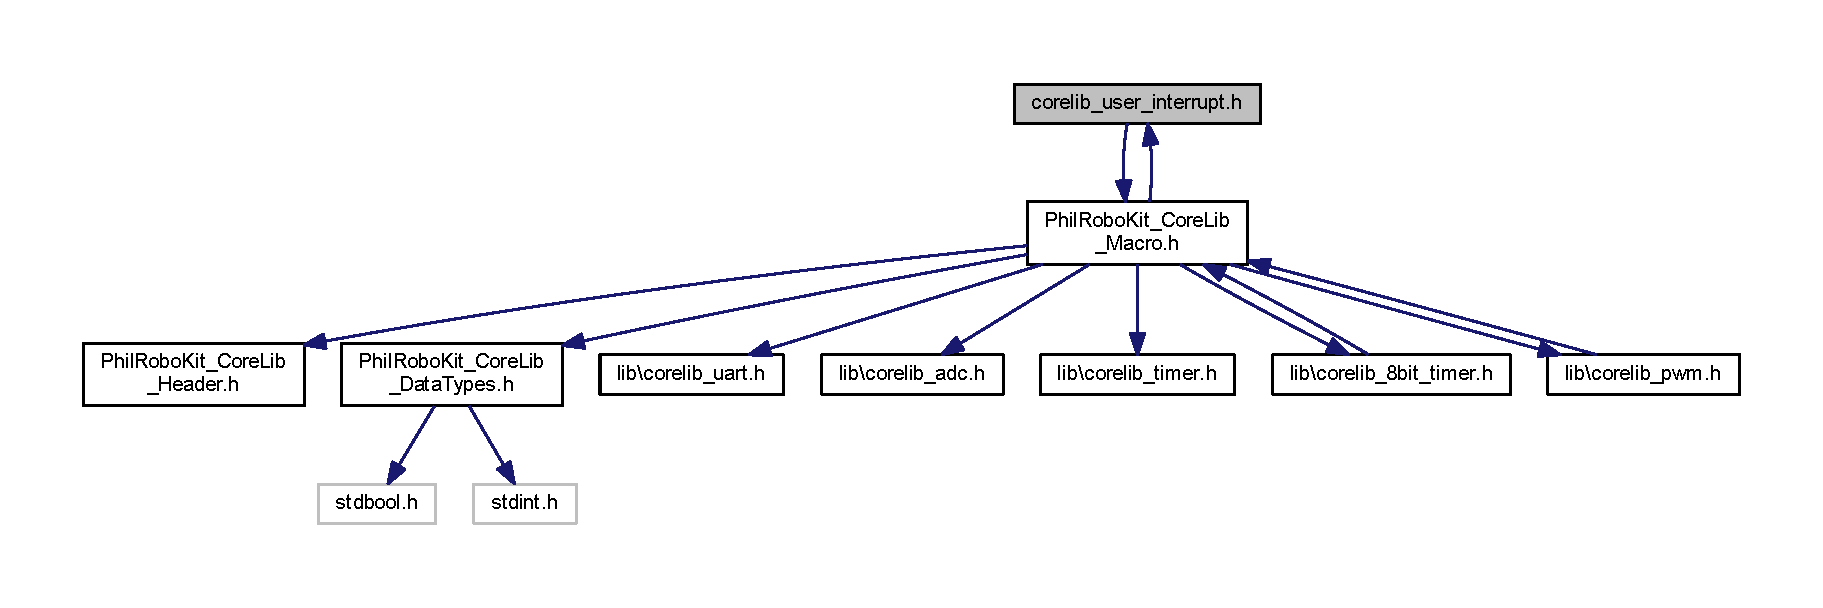
\includegraphics[width=350pt]{corelib__user__interrupt_8h__incl}
\end{center}
\end{figure}
This graph shows which files directly or indirectly include this file\-:\nopagebreak
\begin{figure}[H]
\begin{center}
\leavevmode
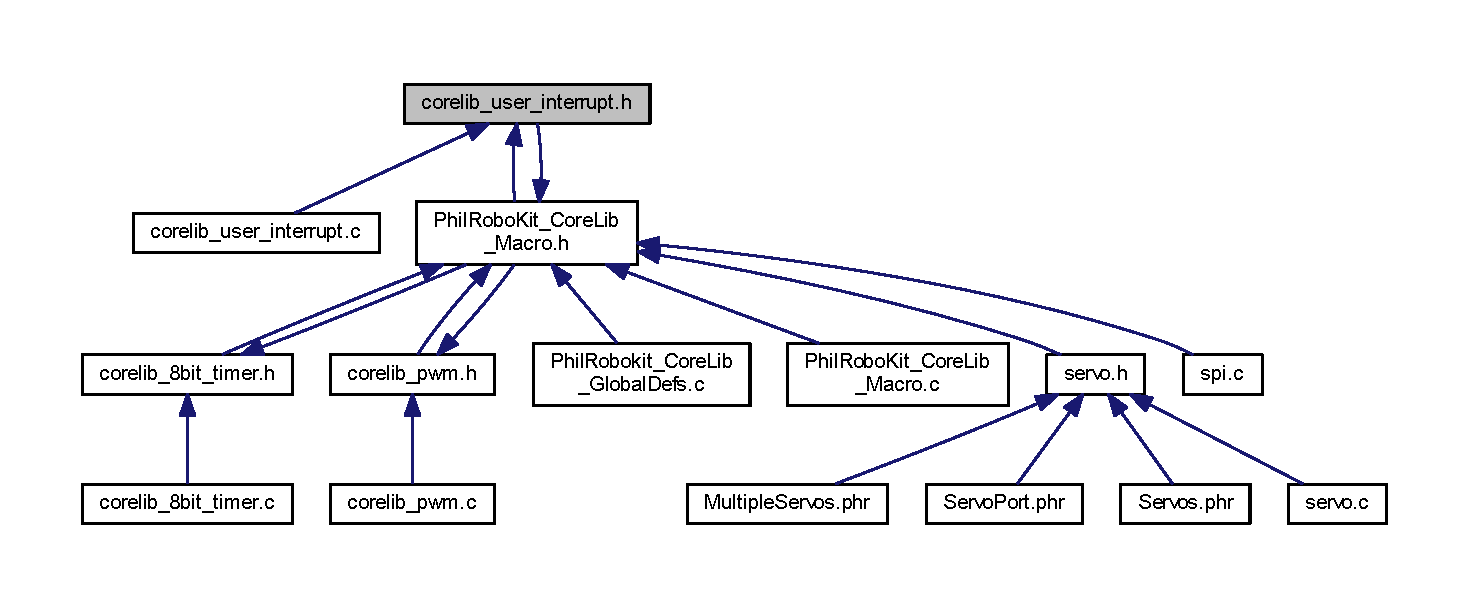
\includegraphics[width=350pt]{corelib__user__interrupt_8h__dep__incl}
\end{center}
\end{figure}
\subsection*{Macros}
\begin{DoxyCompactItemize}
\item 
\#define {\bf E\-X\-T\-I\-N\-T\-E\-N\-A\-B\-L\-E\-D}~{\bf T\-R\-U\-E}
\item 
\#define {\bf R\-B\-I\-N\-T\-E\-N\-A\-B\-L\-E\-D}~{\bf T\-R\-U\-E}
\item 
\#define {\bf R\-B4\-\_\-\-M\-A\-S\-K}~0x10
\item 
\#define {\bf R\-B5\-\_\-\-M\-A\-S\-K}~0x20
\item 
\#define {\bf R\-B6\-\_\-\-M\-A\-S\-K}~0x40
\item 
\#define {\bf R\-B7\-\_\-\-M\-A\-S\-K}~0x80
\end{DoxyCompactItemize}
\subsection*{Enumerations}
\begin{DoxyCompactItemize}
\item 
enum {\bf et\-Interrupt\-Sources} \{ \\*
{\bf I\-N\-T0}, 
{\bf I\-N\-T1}, 
{\bf I\-N\-T2}, 
{\bf I\-N\-T3}, 
\\*
{\bf I\-N\-T4}
 \}
\item 
enum {\bf et\-Interrupt\-Modes} \{ {\bf L\-O\-W\-S\-T\-A\-T\-E}, 
{\bf C\-H\-A\-N\-G\-E}, 
{\bf R\-I\-S\-I\-N\-G}, 
{\bf F\-A\-L\-L\-I\-N\-G}
 \}
\end{DoxyCompactItemize}
\subsection*{Functions}
\begin{DoxyCompactItemize}
\item 
void {\bf setup\-User\-Interrupt} (enum {\bf et\-Interrupt\-Sources} e\-Int\-Source, void($\ast$function)(), enum {\bf et\-Interrupt\-Modes} e\-Int\-Mode)
\item 
void {\bf user\-Interrupt\-Handler} (void)
\end{DoxyCompactItemize}


\subsection{Macro Definition Documentation}
\index{corelib\-\_\-user\-\_\-interrupt.\-h@{corelib\-\_\-user\-\_\-interrupt.\-h}!E\-X\-T\-I\-N\-T\-E\-N\-A\-B\-L\-E\-D@{E\-X\-T\-I\-N\-T\-E\-N\-A\-B\-L\-E\-D}}
\index{E\-X\-T\-I\-N\-T\-E\-N\-A\-B\-L\-E\-D@{E\-X\-T\-I\-N\-T\-E\-N\-A\-B\-L\-E\-D}!corelib_user_interrupt.h@{corelib\-\_\-user\-\_\-interrupt.\-h}}
\subsubsection[{E\-X\-T\-I\-N\-T\-E\-N\-A\-B\-L\-E\-D}]{\setlength{\rightskip}{0pt plus 5cm}\#define E\-X\-T\-I\-N\-T\-E\-N\-A\-B\-L\-E\-D~{\bf T\-R\-U\-E}}\label{corelib__user__interrupt_8h_a07ba89377226d3c36408d7576297952d}


Definition at line 58 of file corelib\-\_\-user\-\_\-interrupt.\-h.

\index{corelib\-\_\-user\-\_\-interrupt.\-h@{corelib\-\_\-user\-\_\-interrupt.\-h}!R\-B4\-\_\-\-M\-A\-S\-K@{R\-B4\-\_\-\-M\-A\-S\-K}}
\index{R\-B4\-\_\-\-M\-A\-S\-K@{R\-B4\-\_\-\-M\-A\-S\-K}!corelib_user_interrupt.h@{corelib\-\_\-user\-\_\-interrupt.\-h}}
\subsubsection[{R\-B4\-\_\-\-M\-A\-S\-K}]{\setlength{\rightskip}{0pt plus 5cm}\#define R\-B4\-\_\-\-M\-A\-S\-K~0x10}\label{corelib__user__interrupt_8h_ad74e927c08dda8f02d1dbd964bc9dbb4}


Definition at line 81 of file corelib\-\_\-user\-\_\-interrupt.\-h.

\index{corelib\-\_\-user\-\_\-interrupt.\-h@{corelib\-\_\-user\-\_\-interrupt.\-h}!R\-B5\-\_\-\-M\-A\-S\-K@{R\-B5\-\_\-\-M\-A\-S\-K}}
\index{R\-B5\-\_\-\-M\-A\-S\-K@{R\-B5\-\_\-\-M\-A\-S\-K}!corelib_user_interrupt.h@{corelib\-\_\-user\-\_\-interrupt.\-h}}
\subsubsection[{R\-B5\-\_\-\-M\-A\-S\-K}]{\setlength{\rightskip}{0pt plus 5cm}\#define R\-B5\-\_\-\-M\-A\-S\-K~0x20}\label{corelib__user__interrupt_8h_a5f50c97535ebf6b0d270010a7e0f2a93}


Definition at line 82 of file corelib\-\_\-user\-\_\-interrupt.\-h.

\index{corelib\-\_\-user\-\_\-interrupt.\-h@{corelib\-\_\-user\-\_\-interrupt.\-h}!R\-B6\-\_\-\-M\-A\-S\-K@{R\-B6\-\_\-\-M\-A\-S\-K}}
\index{R\-B6\-\_\-\-M\-A\-S\-K@{R\-B6\-\_\-\-M\-A\-S\-K}!corelib_user_interrupt.h@{corelib\-\_\-user\-\_\-interrupt.\-h}}
\subsubsection[{R\-B6\-\_\-\-M\-A\-S\-K}]{\setlength{\rightskip}{0pt plus 5cm}\#define R\-B6\-\_\-\-M\-A\-S\-K~0x40}\label{corelib__user__interrupt_8h_ade6c00bc2b304a218e6a0736d626899e}


Definition at line 83 of file corelib\-\_\-user\-\_\-interrupt.\-h.

\index{corelib\-\_\-user\-\_\-interrupt.\-h@{corelib\-\_\-user\-\_\-interrupt.\-h}!R\-B7\-\_\-\-M\-A\-S\-K@{R\-B7\-\_\-\-M\-A\-S\-K}}
\index{R\-B7\-\_\-\-M\-A\-S\-K@{R\-B7\-\_\-\-M\-A\-S\-K}!corelib_user_interrupt.h@{corelib\-\_\-user\-\_\-interrupt.\-h}}
\subsubsection[{R\-B7\-\_\-\-M\-A\-S\-K}]{\setlength{\rightskip}{0pt plus 5cm}\#define R\-B7\-\_\-\-M\-A\-S\-K~0x80}\label{corelib__user__interrupt_8h_a91e2a3a488d20adcd170cb441081eb7e}


Definition at line 84 of file corelib\-\_\-user\-\_\-interrupt.\-h.

\index{corelib\-\_\-user\-\_\-interrupt.\-h@{corelib\-\_\-user\-\_\-interrupt.\-h}!R\-B\-I\-N\-T\-E\-N\-A\-B\-L\-E\-D@{R\-B\-I\-N\-T\-E\-N\-A\-B\-L\-E\-D}}
\index{R\-B\-I\-N\-T\-E\-N\-A\-B\-L\-E\-D@{R\-B\-I\-N\-T\-E\-N\-A\-B\-L\-E\-D}!corelib_user_interrupt.h@{corelib\-\_\-user\-\_\-interrupt.\-h}}
\subsubsection[{R\-B\-I\-N\-T\-E\-N\-A\-B\-L\-E\-D}]{\setlength{\rightskip}{0pt plus 5cm}\#define R\-B\-I\-N\-T\-E\-N\-A\-B\-L\-E\-D~{\bf T\-R\-U\-E}}\label{corelib__user__interrupt_8h_a96c091de2d5653e0b796bcf735092ce0}


Definition at line 59 of file corelib\-\_\-user\-\_\-interrupt.\-h.



\subsection{Enumeration Type Documentation}
\index{corelib\-\_\-user\-\_\-interrupt.\-h@{corelib\-\_\-user\-\_\-interrupt.\-h}!et\-Interrupt\-Modes@{et\-Interrupt\-Modes}}
\index{et\-Interrupt\-Modes@{et\-Interrupt\-Modes}!corelib_user_interrupt.h@{corelib\-\_\-user\-\_\-interrupt.\-h}}
\subsubsection[{et\-Interrupt\-Modes}]{\setlength{\rightskip}{0pt plus 5cm}enum {\bf et\-Interrupt\-Modes}}\label{corelib__user__interrupt_8h_a4f3dc84cee6afc4f663e60ec08656b86}
\begin{Desc}
\item[Enumerator\-: ]\par
\begin{description}
\index{L\-O\-W\-S\-T\-A\-T\-E@{L\-O\-W\-S\-T\-A\-T\-E}!corelib\-\_\-user\-\_\-interrupt.\-h@{corelib\-\_\-user\-\_\-interrupt.\-h}}\index{corelib\-\_\-user\-\_\-interrupt.\-h@{corelib\-\_\-user\-\_\-interrupt.\-h}!L\-O\-W\-S\-T\-A\-T\-E@{L\-O\-W\-S\-T\-A\-T\-E}}\item[{\em 
L\-O\-W\-S\-T\-A\-T\-E\label{corelib__user__interrupt_8h_a4f3dc84cee6afc4f663e60ec08656b86a45509f102e562c86cf17e82564a43e7e}
}]\index{C\-H\-A\-N\-G\-E@{C\-H\-A\-N\-G\-E}!corelib\-\_\-user\-\_\-interrupt.\-h@{corelib\-\_\-user\-\_\-interrupt.\-h}}\index{corelib\-\_\-user\-\_\-interrupt.\-h@{corelib\-\_\-user\-\_\-interrupt.\-h}!C\-H\-A\-N\-G\-E@{C\-H\-A\-N\-G\-E}}\item[{\em 
C\-H\-A\-N\-G\-E\label{corelib__user__interrupt_8h_a4f3dc84cee6afc4f663e60ec08656b86aada6cf2b086af8fd5f84e946d2bd145d}
}]\index{R\-I\-S\-I\-N\-G@{R\-I\-S\-I\-N\-G}!corelib\-\_\-user\-\_\-interrupt.\-h@{corelib\-\_\-user\-\_\-interrupt.\-h}}\index{corelib\-\_\-user\-\_\-interrupt.\-h@{corelib\-\_\-user\-\_\-interrupt.\-h}!R\-I\-S\-I\-N\-G@{R\-I\-S\-I\-N\-G}}\item[{\em 
R\-I\-S\-I\-N\-G\label{corelib__user__interrupt_8h_a4f3dc84cee6afc4f663e60ec08656b86ad93abe7aced82e9a4fcac4127a36ece3}
}]\index{F\-A\-L\-L\-I\-N\-G@{F\-A\-L\-L\-I\-N\-G}!corelib\-\_\-user\-\_\-interrupt.\-h@{corelib\-\_\-user\-\_\-interrupt.\-h}}\index{corelib\-\_\-user\-\_\-interrupt.\-h@{corelib\-\_\-user\-\_\-interrupt.\-h}!F\-A\-L\-L\-I\-N\-G@{F\-A\-L\-L\-I\-N\-G}}\item[{\em 
F\-A\-L\-L\-I\-N\-G\label{corelib__user__interrupt_8h_a4f3dc84cee6afc4f663e60ec08656b86ad24712a6a30c1d431b927d1ba2f84b66}
}]\end{description}
\end{Desc}



Definition at line 72 of file corelib\-\_\-user\-\_\-interrupt.\-h.

\index{corelib\-\_\-user\-\_\-interrupt.\-h@{corelib\-\_\-user\-\_\-interrupt.\-h}!et\-Interrupt\-Sources@{et\-Interrupt\-Sources}}
\index{et\-Interrupt\-Sources@{et\-Interrupt\-Sources}!corelib_user_interrupt.h@{corelib\-\_\-user\-\_\-interrupt.\-h}}
\subsubsection[{et\-Interrupt\-Sources}]{\setlength{\rightskip}{0pt plus 5cm}enum {\bf et\-Interrupt\-Sources}}\label{corelib__user__interrupt_8h_a92939e0f771d15c2c538cea24d952e24}
\begin{Desc}
\item[Enumerator\-: ]\par
\begin{description}
\index{I\-N\-T0@{I\-N\-T0}!corelib\-\_\-user\-\_\-interrupt.\-h@{corelib\-\_\-user\-\_\-interrupt.\-h}}\index{corelib\-\_\-user\-\_\-interrupt.\-h@{corelib\-\_\-user\-\_\-interrupt.\-h}!I\-N\-T0@{I\-N\-T0}}\item[{\em 
I\-N\-T0\label{corelib__user__interrupt_8h_a92939e0f771d15c2c538cea24d952e24a15eea8e66ea11820ade640821d84382d}
}]\index{I\-N\-T1@{I\-N\-T1}!corelib\-\_\-user\-\_\-interrupt.\-h@{corelib\-\_\-user\-\_\-interrupt.\-h}}\index{corelib\-\_\-user\-\_\-interrupt.\-h@{corelib\-\_\-user\-\_\-interrupt.\-h}!I\-N\-T1@{I\-N\-T1}}\item[{\em 
I\-N\-T1\label{corelib__user__interrupt_8h_a92939e0f771d15c2c538cea24d952e24af557cd0d786ab83c4771da6eea65727b}
}]\index{I\-N\-T2@{I\-N\-T2}!corelib\-\_\-user\-\_\-interrupt.\-h@{corelib\-\_\-user\-\_\-interrupt.\-h}}\index{corelib\-\_\-user\-\_\-interrupt.\-h@{corelib\-\_\-user\-\_\-interrupt.\-h}!I\-N\-T2@{I\-N\-T2}}\item[{\em 
I\-N\-T2\label{corelib__user__interrupt_8h_a92939e0f771d15c2c538cea24d952e24ac982725fadf3a115b854a6ff2abaa137}
}]\index{I\-N\-T3@{I\-N\-T3}!corelib\-\_\-user\-\_\-interrupt.\-h@{corelib\-\_\-user\-\_\-interrupt.\-h}}\index{corelib\-\_\-user\-\_\-interrupt.\-h@{corelib\-\_\-user\-\_\-interrupt.\-h}!I\-N\-T3@{I\-N\-T3}}\item[{\em 
I\-N\-T3\label{corelib__user__interrupt_8h_a92939e0f771d15c2c538cea24d952e24a0ad460ad5366d6c276b08550b6a35554}
}]\index{I\-N\-T4@{I\-N\-T4}!corelib\-\_\-user\-\_\-interrupt.\-h@{corelib\-\_\-user\-\_\-interrupt.\-h}}\index{corelib\-\_\-user\-\_\-interrupt.\-h@{corelib\-\_\-user\-\_\-interrupt.\-h}!I\-N\-T4@{I\-N\-T4}}\item[{\em 
I\-N\-T4\label{corelib__user__interrupt_8h_a92939e0f771d15c2c538cea24d952e24a7a8518dedaab44a1a0e0d8ea3c5b567f}
}]\end{description}
\end{Desc}



Definition at line 62 of file corelib\-\_\-user\-\_\-interrupt.\-h.



\subsection{Function Documentation}
\index{corelib\-\_\-user\-\_\-interrupt.\-h@{corelib\-\_\-user\-\_\-interrupt.\-h}!setup\-User\-Interrupt@{setup\-User\-Interrupt}}
\index{setup\-User\-Interrupt@{setup\-User\-Interrupt}!corelib_user_interrupt.h@{corelib\-\_\-user\-\_\-interrupt.\-h}}
\subsubsection[{setup\-User\-Interrupt}]{\setlength{\rightskip}{0pt plus 5cm}void setup\-User\-Interrupt (
\begin{DoxyParamCaption}
\item[{enum {\bf et\-Interrupt\-Sources}}]{e\-Int\-Source, }
\item[{void($\ast$)()}]{function, }
\item[{enum {\bf et\-Interrupt\-Modes}}]{e\-Int\-Mode}
\end{DoxyParamCaption}
)}\label{corelib__user__interrupt_8h_a234efbd3a1dc891dbfbcd0364a9b52ec}


Definition at line 82 of file corelib\-\_\-user\-\_\-interrupt.\-c.

\index{corelib\-\_\-user\-\_\-interrupt.\-h@{corelib\-\_\-user\-\_\-interrupt.\-h}!user\-Interrupt\-Handler@{user\-Interrupt\-Handler}}
\index{user\-Interrupt\-Handler@{user\-Interrupt\-Handler}!corelib_user_interrupt.h@{corelib\-\_\-user\-\_\-interrupt.\-h}}
\subsubsection[{user\-Interrupt\-Handler}]{\setlength{\rightskip}{0pt plus 5cm}void user\-Interrupt\-Handler (
\begin{DoxyParamCaption}
\item[{void}]{}
\end{DoxyParamCaption}
)}\label{corelib__user__interrupt_8h_aa1ef5be24251d01808e5dec4c6babd01}


Definition at line 178 of file corelib\-\_\-user\-\_\-interrupt.\-c.


\section{htc\-\_\-16f87xa.\-h File Reference}
\label{htc__16f87xa_8h}\index{htc\-\_\-16f87xa.\-h@{htc\-\_\-16f87xa.\-h}}
\subsection*{Macros}
\begin{DoxyCompactItemize}
\item 
\#define {\bf R\-E\-G\-I\-S\-T\-E\-R\-\_\-\-T\-X\-S\-T\-A}~T\-X\-S\-T\-A
\item 
\#define {\bf B\-I\-T\-\_\-\-T\-X\-S\-T\-A\-\_\-\-C\-S\-R\-C}~C\-S\-R\-C
\item 
\#define {\bf B\-I\-T\-\_\-\-T\-X\-S\-T\-A\-\_\-\-T\-X9}~T\-X9
\item 
\#define {\bf B\-I\-T\-\_\-\-T\-X\-S\-T\-A\-\_\-\-T\-X\-E\-N}~T\-X\-E\-N
\item 
\#define {\bf B\-I\-T\-\_\-\-T\-X\-S\-T\-A\-\_\-\-S\-Y\-N\-C}~S\-Y\-N\-C
\item 
\#define {\bf B\-I\-T\-\_\-\-T\-X\-S\-T\-A\-\_\-\-B\-R\-G\-H}~B\-R\-G\-H
\item 
\#define {\bf B\-I\-T\-\_\-\-T\-X\-S\-T\-A\-\_\-\-T\-R\-M\-T}~T\-R\-M\-T
\item 
\#define {\bf B\-I\-T\-\_\-\-T\-X\-S\-T\-A\-\_\-\-T\-X9\-D}~T\-X9\-D
\item 
\#define {\bf R\-E\-G\-I\-S\-T\-E\-R\-\_\-\-R\-C\-S\-T\-A}~R\-C\-S\-T\-A
\item 
\#define {\bf B\-I\-T\-\_\-\-R\-C\-S\-T\-A\-\_\-\-S\-P\-E\-N}~S\-P\-E\-N
\item 
\#define {\bf B\-I\-T\-\_\-\-R\-C\-S\-T\-A\-\_\-\-R\-X9}~R\-X9
\item 
\#define {\bf B\-I\-T\-\_\-\-R\-C\-S\-T\-A\-\_\-\-S\-R\-E\-N}~S\-R\-E\-N
\item 
\#define {\bf B\-I\-T\-\_\-\-R\-C\-S\-T\-A\-\_\-\-C\-R\-E\-N}~C\-R\-E\-N
\item 
\#define {\bf B\-I\-T\-\_\-\-R\-C\-S\-T\-A\-\_\-\-A\-D\-D\-E\-N}~A\-D\-D\-E\-N
\item 
\#define {\bf B\-I\-T\-\_\-\-R\-C\-S\-T\-A\-\_\-\-F\-E\-R\-R}~F\-E\-R\-R
\item 
\#define {\bf B\-I\-T\-\_\-\-R\-C\-S\-T\-A\-\_\-\-O\-E\-R\-R}~O\-E\-R\-R
\item 
\#define {\bf B\-I\-T\-\_\-\-R\-C\-S\-T\-A\-\_\-\-R\-X9\-D}~R\-X9\-D
\item 
\#define {\bf R\-E\-G\-I\-S\-T\-E\-R\-\_\-\-I\-N\-T\-C\-O\-N}~I\-N\-T\-C\-O\-N
\item 
\#define {\bf B\-I\-T\-\_\-\-I\-N\-T\-C\-O\-N\-\_\-\-G\-I\-E}~G\-I\-E
\item 
\#define {\bf B\-I\-T\-\_\-\-I\-N\-T\-C\-O\-N\-\_\-\-P\-E\-I\-E}~P\-E\-I\-E
\item 
\#define {\bf B\-I\-T\-\_\-\-I\-N\-T\-C\-O\-N\-\_\-\-T\-M\-R0\-I\-E}~T\-M\-R0\-I\-E
\item 
\#define {\bf B\-I\-T\-\_\-\-I\-N\-T\-C\-O\-N\-\_\-\-I\-N\-T\-E}~I\-N\-T\-E
\item 
\#define {\bf B\-I\-T\-\_\-\-I\-N\-T\-C\-O\-N\-\_\-\-R\-B\-I\-E}~R\-B\-I\-E
\item 
\#define {\bf B\-I\-T\-\_\-\-I\-N\-T\-C\-O\-N\-\_\-\-T\-M\-R0\-I\-F}~T\-M\-R0\-I\-F
\item 
\#define {\bf B\-I\-T\-\_\-\-I\-N\-T\-C\-O\-N\-\_\-\-I\-N\-T\-F}~I\-N\-T\-F
\item 
\#define {\bf B\-I\-T\-\_\-\-I\-N\-T\-C\-O\-N\-\_\-\-R\-B\-I\-F}~R\-B\-I\-F
\item 
\#define {\bf R\-E\-G\-I\-S\-T\-E\-R\-\_\-\-P\-I\-R1}~P\-I\-R1
\item 
\#define {\bf B\-I\-T\-\_\-\-P\-I\-R1\-\_\-\-P\-S\-P\-I\-F}~P\-S\-P\-I\-F
\item 
\#define {\bf B\-I\-T\-\_\-\-P\-I\-R1\-\_\-\-A\-D\-I\-F}~A\-D\-I\-F
\item 
\#define {\bf B\-I\-T\-\_\-\-P\-I\-R1\-\_\-\-R\-C\-I\-F}~R\-C\-I\-F
\item 
\#define {\bf B\-I\-T\-\_\-\-P\-I\-R1\-\_\-\-T\-X\-I\-F}~T\-X\-I\-F
\item 
\#define {\bf B\-I\-T\-\_\-\-P\-I\-R1\-\_\-\-S\-S\-P\-I\-F}~S\-P\-I\-F
\item 
\#define {\bf B\-I\-T\-\_\-\-P\-I\-R1\-\_\-\-C\-C\-P1\-I\-F}~C\-C\-P1\-I\-F
\item 
\#define {\bf B\-I\-T\-\_\-\-P\-I\-R1\-\_\-\-T\-M\-R2\-I\-F}~T\-M\-R2\-I\-F
\item 
\#define {\bf B\-I\-T\-\_\-\-P\-I\-R1\-\_\-\-T\-M\-R1\-I\-F}~T\-M\-R1\-I\-F
\item 
\#define {\bf R\-E\-G\-I\-S\-T\-E\-R\-\_\-\-P\-I\-E1}~P\-I\-E1
\item 
\#define {\bf B\-I\-T\-\_\-\-P\-I\-E1\-\_\-\-P\-S\-P\-I\-E}~P\-S\-P\-I\-E
\item 
\#define {\bf B\-I\-T\-\_\-\-P\-I\-E1\-\_\-\-A\-D\-I\-E}~A\-D\-I\-E
\item 
\#define {\bf B\-I\-T\-\_\-\-P\-I\-E1\-\_\-\-R\-C\-I\-E}~R\-C\-I\-E
\item 
\#define {\bf B\-I\-T\-\_\-\-P\-I\-E1\-\_\-\-T\-X\-I\-E}~T\-X\-I\-E
\item 
\#define {\bf B\-I\-T\-\_\-\-P\-I\-E1\-\_\-\-S\-S\-P\-I\-E}~S\-S\-P\-I\-E
\item 
\#define {\bf B\-I\-T\-\_\-\-P\-I\-E1\-\_\-\-C\-C\-P1\-I\-E}~C\-C\-P1\-I\-E
\item 
\#define {\bf B\-I\-T\-\_\-\-P\-I\-E1\-\_\-\-T\-M\-R2\-I\-E}~T\-M\-R2\-I\-E
\item 
\#define {\bf B\-I\-T\-\_\-\-P\-I\-E1\-\_\-\-T\-M\-R1\-I\-E}~T\-M\-R1\-I\-E
\item 
\#define {\bf R\-E\-G\-I\-S\-T\-E\-R\-\_\-\-T1\-C\-O\-N}~T1\-C\-O\-N
\item 
\#define {\bf B\-I\-T\-\_\-\-T1\-C\-O\-N\-\_\-\-T1\-C\-K\-P\-S1}~T1\-C\-K\-P\-S1
\item 
\#define {\bf B\-I\-T\-\_\-\-T1\-C\-O\-N\-\_\-\-T1\-C\-K\-P\-S0}~T1\-C\-K\-P\-S0
\item 
\#define {\bf B\-I\-T\-\_\-\-T1\-C\-O\-N\-\_\-\-T1\-O\-S\-C\-E\-N}~T1\-O\-S\-C\-E\-N
\item 
\#define {\bf B\-I\-T\-\_\-\-T1\-C\-O\-N\-\_\-\-T1\-S\-Y\-N\-C}~T1\-S\-Y\-N\-C
\item 
\#define {\bf B\-I\-T\-\_\-\-T1\-C\-O\-N\-\_\-\-T\-M\-R1\-C\-S}~T\-M\-R1\-C\-S
\item 
\#define {\bf B\-I\-T\-\_\-\-T1\-C\-O\-N\-\_\-\-T\-M\-R1\-O\-N}~T\-M\-R1\-O\-N
\item 
\#define {\bf R\-E\-G\-I\-S\-T\-E\-R\-\_\-\-A\-D\-C\-O\-N0}~A\-D\-C\-O\-N0
\item 
\#define {\bf B\-I\-T\-\_\-\-A\-D\-C\-O\-N0\-\_\-\-A\-D\-C\-S1}~A\-D\-C\-S1
\item 
\#define {\bf B\-I\-T\-\_\-\-A\-D\-C\-O\-N0\-\_\-\-A\-D\-C\-S0}~A\-D\-C\-S0
\item 
\#define {\bf B\-I\-T\-\_\-\-A\-D\-C\-O\-N0\-\_\-\-C\-H\-S2}~C\-H\-S2
\item 
\#define {\bf B\-I\-T\-\_\-\-A\-D\-C\-O\-N0\-\_\-\-C\-H\-S1}~C\-H\-S1
\item 
\#define {\bf B\-I\-T\-\_\-\-A\-D\-C\-O\-N0\-\_\-\-C\-H\-S0}~C\-H\-S0
\item 
\#define {\bf B\-I\-T\-\_\-\-A\-D\-C\-O\-N0\-\_\-\-G\-O\-\_\-\-D\-O\-N\-E}~G\-O\-\_\-\-D\-O\-N\-E
\item 
\#define {\bf B\-I\-T\-\_\-\-A\-D\-C\-O\-N0\-\_\-\-A\-D\-O\-N}~A\-D\-O\-N
\item 
\#define {\bf R\-E\-G\-I\-S\-T\-E\-R\-\_\-\-A\-D\-C\-O\-N1}~A\-D\-C\-O\-N1
\item 
\#define {\bf B\-I\-T\-\_\-\-A\-D\-C\-O\-N1\-\_\-\-A\-D\-F\-M}~A\-D\-F\-M
\item 
\#define {\bf B\-I\-T\-\_\-\-A\-D\-C\-O\-N1\-\_\-\-A\-D\-C\-S2}~A\-D\-C\-S2
\item 
\#define {\bf B\-I\-T\-\_\-\-A\-D\-C\-O\-N1\-\_\-\-P\-C\-F\-G3}~P\-C\-F\-G3
\item 
\#define {\bf B\-I\-T\-\_\-\-A\-D\-C\-O\-N1\-\_\-\-P\-C\-F\-G2}~P\-C\-F\-G2
\item 
\#define {\bf B\-I\-T\-\_\-\-A\-D\-C\-O\-N1\-\_\-\-P\-C\-F\-G1}~P\-C\-F\-G1
\item 
\#define {\bf B\-I\-T\-\_\-\-A\-D\-C\-O\-N1\-\_\-\-P\-C\-F\-G0}~P\-C\-F\-G0
\item 
\#define {\bf R\-E\-G\-I\-S\-T\-E\-R\-\_\-\-P\-R2}~P\-R2
\item 
\#define {\bf R\-E\-G\-I\-S\-T\-E\-R\-\_\-\-T2\-C\-O\-N}~T2\-C\-O\-N
\item 
\#define {\bf B\-I\-T\-\_\-\-T2\-C\-O\-N\-\_\-\-T\-O\-U\-T\-P\-S3}~T\-O\-U\-T\-P\-S3
\item 
\#define {\bf B\-I\-T\-\_\-\-T2\-C\-O\-N\-\_\-\-T\-O\-U\-T\-P\-S2}~T\-O\-U\-T\-P\-S2
\item 
\#define {\bf B\-I\-T\-\_\-\-T2\-C\-O\-N\-\_\-\-T\-O\-U\-T\-P\-S1}~T\-O\-U\-T\-P\-S1
\item 
\#define {\bf B\-I\-T\-\_\-\-T2\-C\-O\-N\-\_\-\-T\-O\-U\-T\-P\-S0}~T\-O\-U\-T\-P\-S0
\item 
\#define {\bf B\-I\-T\-\_\-\-T2\-C\-O\-N\-\_\-\-T\-M\-R2\-O\-N}~T\-M\-R2\-O\-N
\item 
\#define {\bf B\-I\-T\-\_\-\-T2\-C\-O\-N\-\_\-\-T2\-C\-K\-P\-S1}~T2\-C\-K\-P\-S1
\item 
\#define {\bf B\-I\-T\-\_\-\-T2\-C\-O\-N\-\_\-\-T2\-C\-K\-P\-S0}~T2\-C\-K\-P\-S0
\item 
\#define {\bf T\-M\-R\-\_\-\-P\-O\-S\-T\-S\-C\-A\-L\-E\-\_\-\-M\-A\-S\-K}~0x78
\item 
\#define {\bf T\-M\-R\-\_\-\-P\-R\-E\-S\-C\-A\-L\-E\-\_\-\-M\-A\-S\-K}~0x03
\item 
\#define {\bf R\-E\-G\-I\-S\-T\-E\-R\-\_\-\-C\-C\-P1\-C\-O\-N}~C\-C\-P1\-C\-O\-N
\item 
\#define {\bf R\-E\-G\-I\-S\-T\-E\-R\-\_\-\-C\-C\-P2\-C\-O\-N}~C\-C\-P2\-C\-O\-N
\item 
\#define {\bf M\-A\-S\-K\-\_\-\-Px\-M1}~0x80
\item 
\#define {\bf M\-A\-S\-K\-\_\-\-Px\-M0}~0x40
\item 
\#define {\bf M\-A\-S\-K\-\_\-\-D\-Cx\-B1}~0x20
\item 
\#define {\bf M\-A\-S\-K\-\_\-\-D\-Cx\-B0}~0x10
\item 
\#define {\bf M\-A\-S\-K\-\_\-\-C\-C\-Px\-M3}~0x08
\item 
\#define {\bf M\-A\-S\-K\-\_\-\-C\-C\-Px\-M2}~0x04
\item 
\#define {\bf M\-A\-S\-K\-\_\-\-C\-C\-Px\-M1}~0x02
\item 
\#define {\bf M\-A\-S\-K\-\_\-\-C\-C\-Px\-M0}~0x01
\item 
\#define {\bf E\-C\-C\-P\-\_\-\-C\-O\-N\-F\-I\-G\-\_\-\-M\-A\-S\-K}~0x\-C0
\item 
\#define {\bf P\-W\-M\-\_\-\-D\-C\-\_\-\-L\-S\-B\-\_\-\-M\-A\-S\-K}~0x30
\item 
\#define {\bf C\-C\-P\-\_\-\-M\-O\-D\-E\-\_\-\-M\-A\-S\-K}~0x0\-F
\item 
\#define {\bf R\-E\-G\-I\-S\-T\-E\-R\-\_\-\-C\-C\-P\-R1\-L}~C\-C\-P\-R1\-L
\item 
\#define {\bf R\-E\-G\-I\-S\-T\-E\-R\-\_\-\-C\-C\-P\-R2\-L}~C\-C\-P\-R2\-L
\end{DoxyCompactItemize}


\subsection{Macro Definition Documentation}
\index{htc\-\_\-16f87xa.\-h@{htc\-\_\-16f87xa.\-h}!B\-I\-T\-\_\-\-A\-D\-C\-O\-N0\-\_\-\-A\-D\-C\-S0@{B\-I\-T\-\_\-\-A\-D\-C\-O\-N0\-\_\-\-A\-D\-C\-S0}}
\index{B\-I\-T\-\_\-\-A\-D\-C\-O\-N0\-\_\-\-A\-D\-C\-S0@{B\-I\-T\-\_\-\-A\-D\-C\-O\-N0\-\_\-\-A\-D\-C\-S0}!htc_16f87xa.h@{htc\-\_\-16f87xa.\-h}}
\subsubsection[{B\-I\-T\-\_\-\-A\-D\-C\-O\-N0\-\_\-\-A\-D\-C\-S0}]{\setlength{\rightskip}{0pt plus 5cm}\#define B\-I\-T\-\_\-\-A\-D\-C\-O\-N0\-\_\-\-A\-D\-C\-S0~A\-D\-C\-S0}\label{htc__16f87xa_8h_ac01da456d82b8e7b60dd86924eff1388}


Definition at line 96 of file htc\-\_\-16f87xa.\-h.

\index{htc\-\_\-16f87xa.\-h@{htc\-\_\-16f87xa.\-h}!B\-I\-T\-\_\-\-A\-D\-C\-O\-N0\-\_\-\-A\-D\-C\-S1@{B\-I\-T\-\_\-\-A\-D\-C\-O\-N0\-\_\-\-A\-D\-C\-S1}}
\index{B\-I\-T\-\_\-\-A\-D\-C\-O\-N0\-\_\-\-A\-D\-C\-S1@{B\-I\-T\-\_\-\-A\-D\-C\-O\-N0\-\_\-\-A\-D\-C\-S1}!htc_16f87xa.h@{htc\-\_\-16f87xa.\-h}}
\subsubsection[{B\-I\-T\-\_\-\-A\-D\-C\-O\-N0\-\_\-\-A\-D\-C\-S1}]{\setlength{\rightskip}{0pt plus 5cm}\#define B\-I\-T\-\_\-\-A\-D\-C\-O\-N0\-\_\-\-A\-D\-C\-S1~A\-D\-C\-S1}\label{htc__16f87xa_8h_abd27a42001108931cf843e1daee57347}


Definition at line 95 of file htc\-\_\-16f87xa.\-h.

\index{htc\-\_\-16f87xa.\-h@{htc\-\_\-16f87xa.\-h}!B\-I\-T\-\_\-\-A\-D\-C\-O\-N0\-\_\-\-A\-D\-O\-N@{B\-I\-T\-\_\-\-A\-D\-C\-O\-N0\-\_\-\-A\-D\-O\-N}}
\index{B\-I\-T\-\_\-\-A\-D\-C\-O\-N0\-\_\-\-A\-D\-O\-N@{B\-I\-T\-\_\-\-A\-D\-C\-O\-N0\-\_\-\-A\-D\-O\-N}!htc_16f87xa.h@{htc\-\_\-16f87xa.\-h}}
\subsubsection[{B\-I\-T\-\_\-\-A\-D\-C\-O\-N0\-\_\-\-A\-D\-O\-N}]{\setlength{\rightskip}{0pt plus 5cm}\#define B\-I\-T\-\_\-\-A\-D\-C\-O\-N0\-\_\-\-A\-D\-O\-N~A\-D\-O\-N}\label{htc__16f87xa_8h_a3be7a8cac4e8a4b8331a73e489550039}


Definition at line 102 of file htc\-\_\-16f87xa.\-h.

\index{htc\-\_\-16f87xa.\-h@{htc\-\_\-16f87xa.\-h}!B\-I\-T\-\_\-\-A\-D\-C\-O\-N0\-\_\-\-C\-H\-S0@{B\-I\-T\-\_\-\-A\-D\-C\-O\-N0\-\_\-\-C\-H\-S0}}
\index{B\-I\-T\-\_\-\-A\-D\-C\-O\-N0\-\_\-\-C\-H\-S0@{B\-I\-T\-\_\-\-A\-D\-C\-O\-N0\-\_\-\-C\-H\-S0}!htc_16f87xa.h@{htc\-\_\-16f87xa.\-h}}
\subsubsection[{B\-I\-T\-\_\-\-A\-D\-C\-O\-N0\-\_\-\-C\-H\-S0}]{\setlength{\rightskip}{0pt plus 5cm}\#define B\-I\-T\-\_\-\-A\-D\-C\-O\-N0\-\_\-\-C\-H\-S0~C\-H\-S0}\label{htc__16f87xa_8h_ac52fd4eeb36398b39349d87d0d25798c}


Definition at line 99 of file htc\-\_\-16f87xa.\-h.

\index{htc\-\_\-16f87xa.\-h@{htc\-\_\-16f87xa.\-h}!B\-I\-T\-\_\-\-A\-D\-C\-O\-N0\-\_\-\-C\-H\-S1@{B\-I\-T\-\_\-\-A\-D\-C\-O\-N0\-\_\-\-C\-H\-S1}}
\index{B\-I\-T\-\_\-\-A\-D\-C\-O\-N0\-\_\-\-C\-H\-S1@{B\-I\-T\-\_\-\-A\-D\-C\-O\-N0\-\_\-\-C\-H\-S1}!htc_16f87xa.h@{htc\-\_\-16f87xa.\-h}}
\subsubsection[{B\-I\-T\-\_\-\-A\-D\-C\-O\-N0\-\_\-\-C\-H\-S1}]{\setlength{\rightskip}{0pt plus 5cm}\#define B\-I\-T\-\_\-\-A\-D\-C\-O\-N0\-\_\-\-C\-H\-S1~C\-H\-S1}\label{htc__16f87xa_8h_a2413e85c16b4481b8d7d7d6ba2077d5f}


Definition at line 98 of file htc\-\_\-16f87xa.\-h.

\index{htc\-\_\-16f87xa.\-h@{htc\-\_\-16f87xa.\-h}!B\-I\-T\-\_\-\-A\-D\-C\-O\-N0\-\_\-\-C\-H\-S2@{B\-I\-T\-\_\-\-A\-D\-C\-O\-N0\-\_\-\-C\-H\-S2}}
\index{B\-I\-T\-\_\-\-A\-D\-C\-O\-N0\-\_\-\-C\-H\-S2@{B\-I\-T\-\_\-\-A\-D\-C\-O\-N0\-\_\-\-C\-H\-S2}!htc_16f87xa.h@{htc\-\_\-16f87xa.\-h}}
\subsubsection[{B\-I\-T\-\_\-\-A\-D\-C\-O\-N0\-\_\-\-C\-H\-S2}]{\setlength{\rightskip}{0pt plus 5cm}\#define B\-I\-T\-\_\-\-A\-D\-C\-O\-N0\-\_\-\-C\-H\-S2~C\-H\-S2}\label{htc__16f87xa_8h_a0b895c3a420beecb15aeeb9237066b4b}


Definition at line 97 of file htc\-\_\-16f87xa.\-h.

\index{htc\-\_\-16f87xa.\-h@{htc\-\_\-16f87xa.\-h}!B\-I\-T\-\_\-\-A\-D\-C\-O\-N0\-\_\-\-G\-O\-\_\-\-D\-O\-N\-E@{B\-I\-T\-\_\-\-A\-D\-C\-O\-N0\-\_\-\-G\-O\-\_\-\-D\-O\-N\-E}}
\index{B\-I\-T\-\_\-\-A\-D\-C\-O\-N0\-\_\-\-G\-O\-\_\-\-D\-O\-N\-E@{B\-I\-T\-\_\-\-A\-D\-C\-O\-N0\-\_\-\-G\-O\-\_\-\-D\-O\-N\-E}!htc_16f87xa.h@{htc\-\_\-16f87xa.\-h}}
\subsubsection[{B\-I\-T\-\_\-\-A\-D\-C\-O\-N0\-\_\-\-G\-O\-\_\-\-D\-O\-N\-E}]{\setlength{\rightskip}{0pt plus 5cm}\#define B\-I\-T\-\_\-\-A\-D\-C\-O\-N0\-\_\-\-G\-O\-\_\-\-D\-O\-N\-E~G\-O\-\_\-\-D\-O\-N\-E}\label{htc__16f87xa_8h_a86cf308db34efc38b913d5de770b840f}


Definition at line 100 of file htc\-\_\-16f87xa.\-h.

\index{htc\-\_\-16f87xa.\-h@{htc\-\_\-16f87xa.\-h}!B\-I\-T\-\_\-\-A\-D\-C\-O\-N1\-\_\-\-A\-D\-C\-S2@{B\-I\-T\-\_\-\-A\-D\-C\-O\-N1\-\_\-\-A\-D\-C\-S2}}
\index{B\-I\-T\-\_\-\-A\-D\-C\-O\-N1\-\_\-\-A\-D\-C\-S2@{B\-I\-T\-\_\-\-A\-D\-C\-O\-N1\-\_\-\-A\-D\-C\-S2}!htc_16f87xa.h@{htc\-\_\-16f87xa.\-h}}
\subsubsection[{B\-I\-T\-\_\-\-A\-D\-C\-O\-N1\-\_\-\-A\-D\-C\-S2}]{\setlength{\rightskip}{0pt plus 5cm}\#define B\-I\-T\-\_\-\-A\-D\-C\-O\-N1\-\_\-\-A\-D\-C\-S2~A\-D\-C\-S2}\label{htc__16f87xa_8h_a9f4d0ccfb8e554e89b6e3925dd105b59}


Definition at line 106 of file htc\-\_\-16f87xa.\-h.

\index{htc\-\_\-16f87xa.\-h@{htc\-\_\-16f87xa.\-h}!B\-I\-T\-\_\-\-A\-D\-C\-O\-N1\-\_\-\-A\-D\-F\-M@{B\-I\-T\-\_\-\-A\-D\-C\-O\-N1\-\_\-\-A\-D\-F\-M}}
\index{B\-I\-T\-\_\-\-A\-D\-C\-O\-N1\-\_\-\-A\-D\-F\-M@{B\-I\-T\-\_\-\-A\-D\-C\-O\-N1\-\_\-\-A\-D\-F\-M}!htc_16f87xa.h@{htc\-\_\-16f87xa.\-h}}
\subsubsection[{B\-I\-T\-\_\-\-A\-D\-C\-O\-N1\-\_\-\-A\-D\-F\-M}]{\setlength{\rightskip}{0pt plus 5cm}\#define B\-I\-T\-\_\-\-A\-D\-C\-O\-N1\-\_\-\-A\-D\-F\-M~A\-D\-F\-M}\label{htc__16f87xa_8h_a8d8f3cb5d3cb7dcf1d8d4ecfc3e6326a}


Definition at line 105 of file htc\-\_\-16f87xa.\-h.

\index{htc\-\_\-16f87xa.\-h@{htc\-\_\-16f87xa.\-h}!B\-I\-T\-\_\-\-A\-D\-C\-O\-N1\-\_\-\-P\-C\-F\-G0@{B\-I\-T\-\_\-\-A\-D\-C\-O\-N1\-\_\-\-P\-C\-F\-G0}}
\index{B\-I\-T\-\_\-\-A\-D\-C\-O\-N1\-\_\-\-P\-C\-F\-G0@{B\-I\-T\-\_\-\-A\-D\-C\-O\-N1\-\_\-\-P\-C\-F\-G0}!htc_16f87xa.h@{htc\-\_\-16f87xa.\-h}}
\subsubsection[{B\-I\-T\-\_\-\-A\-D\-C\-O\-N1\-\_\-\-P\-C\-F\-G0}]{\setlength{\rightskip}{0pt plus 5cm}\#define B\-I\-T\-\_\-\-A\-D\-C\-O\-N1\-\_\-\-P\-C\-F\-G0~P\-C\-F\-G0}\label{htc__16f87xa_8h_aec94078e19090bfb7308b5d176d3b53f}


Definition at line 112 of file htc\-\_\-16f87xa.\-h.

\index{htc\-\_\-16f87xa.\-h@{htc\-\_\-16f87xa.\-h}!B\-I\-T\-\_\-\-A\-D\-C\-O\-N1\-\_\-\-P\-C\-F\-G1@{B\-I\-T\-\_\-\-A\-D\-C\-O\-N1\-\_\-\-P\-C\-F\-G1}}
\index{B\-I\-T\-\_\-\-A\-D\-C\-O\-N1\-\_\-\-P\-C\-F\-G1@{B\-I\-T\-\_\-\-A\-D\-C\-O\-N1\-\_\-\-P\-C\-F\-G1}!htc_16f87xa.h@{htc\-\_\-16f87xa.\-h}}
\subsubsection[{B\-I\-T\-\_\-\-A\-D\-C\-O\-N1\-\_\-\-P\-C\-F\-G1}]{\setlength{\rightskip}{0pt plus 5cm}\#define B\-I\-T\-\_\-\-A\-D\-C\-O\-N1\-\_\-\-P\-C\-F\-G1~P\-C\-F\-G1}\label{htc__16f87xa_8h_a7f52f99066bad8a63d30b97d772a8eb0}


Definition at line 111 of file htc\-\_\-16f87xa.\-h.

\index{htc\-\_\-16f87xa.\-h@{htc\-\_\-16f87xa.\-h}!B\-I\-T\-\_\-\-A\-D\-C\-O\-N1\-\_\-\-P\-C\-F\-G2@{B\-I\-T\-\_\-\-A\-D\-C\-O\-N1\-\_\-\-P\-C\-F\-G2}}
\index{B\-I\-T\-\_\-\-A\-D\-C\-O\-N1\-\_\-\-P\-C\-F\-G2@{B\-I\-T\-\_\-\-A\-D\-C\-O\-N1\-\_\-\-P\-C\-F\-G2}!htc_16f87xa.h@{htc\-\_\-16f87xa.\-h}}
\subsubsection[{B\-I\-T\-\_\-\-A\-D\-C\-O\-N1\-\_\-\-P\-C\-F\-G2}]{\setlength{\rightskip}{0pt plus 5cm}\#define B\-I\-T\-\_\-\-A\-D\-C\-O\-N1\-\_\-\-P\-C\-F\-G2~P\-C\-F\-G2}\label{htc__16f87xa_8h_ad90974d9ff6daa98b102da59a7165d8b}


Definition at line 110 of file htc\-\_\-16f87xa.\-h.

\index{htc\-\_\-16f87xa.\-h@{htc\-\_\-16f87xa.\-h}!B\-I\-T\-\_\-\-A\-D\-C\-O\-N1\-\_\-\-P\-C\-F\-G3@{B\-I\-T\-\_\-\-A\-D\-C\-O\-N1\-\_\-\-P\-C\-F\-G3}}
\index{B\-I\-T\-\_\-\-A\-D\-C\-O\-N1\-\_\-\-P\-C\-F\-G3@{B\-I\-T\-\_\-\-A\-D\-C\-O\-N1\-\_\-\-P\-C\-F\-G3}!htc_16f87xa.h@{htc\-\_\-16f87xa.\-h}}
\subsubsection[{B\-I\-T\-\_\-\-A\-D\-C\-O\-N1\-\_\-\-P\-C\-F\-G3}]{\setlength{\rightskip}{0pt plus 5cm}\#define B\-I\-T\-\_\-\-A\-D\-C\-O\-N1\-\_\-\-P\-C\-F\-G3~P\-C\-F\-G3}\label{htc__16f87xa_8h_a58e73d3f6ae4d1c356bfc5fb17e16729}


Definition at line 109 of file htc\-\_\-16f87xa.\-h.

\index{htc\-\_\-16f87xa.\-h@{htc\-\_\-16f87xa.\-h}!B\-I\-T\-\_\-\-I\-N\-T\-C\-O\-N\-\_\-\-G\-I\-E@{B\-I\-T\-\_\-\-I\-N\-T\-C\-O\-N\-\_\-\-G\-I\-E}}
\index{B\-I\-T\-\_\-\-I\-N\-T\-C\-O\-N\-\_\-\-G\-I\-E@{B\-I\-T\-\_\-\-I\-N\-T\-C\-O\-N\-\_\-\-G\-I\-E}!htc_16f87xa.h@{htc\-\_\-16f87xa.\-h}}
\subsubsection[{B\-I\-T\-\_\-\-I\-N\-T\-C\-O\-N\-\_\-\-G\-I\-E}]{\setlength{\rightskip}{0pt plus 5cm}\#define B\-I\-T\-\_\-\-I\-N\-T\-C\-O\-N\-\_\-\-G\-I\-E~G\-I\-E}\label{htc__16f87xa_8h_a1125281be43753eb6d7f01a0d610f2dc}


Definition at line 55 of file htc\-\_\-16f87xa.\-h.

\index{htc\-\_\-16f87xa.\-h@{htc\-\_\-16f87xa.\-h}!B\-I\-T\-\_\-\-I\-N\-T\-C\-O\-N\-\_\-\-I\-N\-T\-E@{B\-I\-T\-\_\-\-I\-N\-T\-C\-O\-N\-\_\-\-I\-N\-T\-E}}
\index{B\-I\-T\-\_\-\-I\-N\-T\-C\-O\-N\-\_\-\-I\-N\-T\-E@{B\-I\-T\-\_\-\-I\-N\-T\-C\-O\-N\-\_\-\-I\-N\-T\-E}!htc_16f87xa.h@{htc\-\_\-16f87xa.\-h}}
\subsubsection[{B\-I\-T\-\_\-\-I\-N\-T\-C\-O\-N\-\_\-\-I\-N\-T\-E}]{\setlength{\rightskip}{0pt plus 5cm}\#define B\-I\-T\-\_\-\-I\-N\-T\-C\-O\-N\-\_\-\-I\-N\-T\-E~I\-N\-T\-E}\label{htc__16f87xa_8h_aa674071db71ca06d2c643d9146cc960e}


Definition at line 58 of file htc\-\_\-16f87xa.\-h.

\index{htc\-\_\-16f87xa.\-h@{htc\-\_\-16f87xa.\-h}!B\-I\-T\-\_\-\-I\-N\-T\-C\-O\-N\-\_\-\-I\-N\-T\-F@{B\-I\-T\-\_\-\-I\-N\-T\-C\-O\-N\-\_\-\-I\-N\-T\-F}}
\index{B\-I\-T\-\_\-\-I\-N\-T\-C\-O\-N\-\_\-\-I\-N\-T\-F@{B\-I\-T\-\_\-\-I\-N\-T\-C\-O\-N\-\_\-\-I\-N\-T\-F}!htc_16f87xa.h@{htc\-\_\-16f87xa.\-h}}
\subsubsection[{B\-I\-T\-\_\-\-I\-N\-T\-C\-O\-N\-\_\-\-I\-N\-T\-F}]{\setlength{\rightskip}{0pt plus 5cm}\#define B\-I\-T\-\_\-\-I\-N\-T\-C\-O\-N\-\_\-\-I\-N\-T\-F~I\-N\-T\-F}\label{htc__16f87xa_8h_a092a7af47d6867d625139e1fb3274914}


Definition at line 61 of file htc\-\_\-16f87xa.\-h.

\index{htc\-\_\-16f87xa.\-h@{htc\-\_\-16f87xa.\-h}!B\-I\-T\-\_\-\-I\-N\-T\-C\-O\-N\-\_\-\-P\-E\-I\-E@{B\-I\-T\-\_\-\-I\-N\-T\-C\-O\-N\-\_\-\-P\-E\-I\-E}}
\index{B\-I\-T\-\_\-\-I\-N\-T\-C\-O\-N\-\_\-\-P\-E\-I\-E@{B\-I\-T\-\_\-\-I\-N\-T\-C\-O\-N\-\_\-\-P\-E\-I\-E}!htc_16f87xa.h@{htc\-\_\-16f87xa.\-h}}
\subsubsection[{B\-I\-T\-\_\-\-I\-N\-T\-C\-O\-N\-\_\-\-P\-E\-I\-E}]{\setlength{\rightskip}{0pt plus 5cm}\#define B\-I\-T\-\_\-\-I\-N\-T\-C\-O\-N\-\_\-\-P\-E\-I\-E~P\-E\-I\-E}\label{htc__16f87xa_8h_adcdb6145b4e354273a9836e1621d203b}


Definition at line 56 of file htc\-\_\-16f87xa.\-h.

\index{htc\-\_\-16f87xa.\-h@{htc\-\_\-16f87xa.\-h}!B\-I\-T\-\_\-\-I\-N\-T\-C\-O\-N\-\_\-\-R\-B\-I\-E@{B\-I\-T\-\_\-\-I\-N\-T\-C\-O\-N\-\_\-\-R\-B\-I\-E}}
\index{B\-I\-T\-\_\-\-I\-N\-T\-C\-O\-N\-\_\-\-R\-B\-I\-E@{B\-I\-T\-\_\-\-I\-N\-T\-C\-O\-N\-\_\-\-R\-B\-I\-E}!htc_16f87xa.h@{htc\-\_\-16f87xa.\-h}}
\subsubsection[{B\-I\-T\-\_\-\-I\-N\-T\-C\-O\-N\-\_\-\-R\-B\-I\-E}]{\setlength{\rightskip}{0pt plus 5cm}\#define B\-I\-T\-\_\-\-I\-N\-T\-C\-O\-N\-\_\-\-R\-B\-I\-E~R\-B\-I\-E}\label{htc__16f87xa_8h_ac4d3b2cf1b09a5b60a6ff3fae4d0cd7d}


Definition at line 59 of file htc\-\_\-16f87xa.\-h.

\index{htc\-\_\-16f87xa.\-h@{htc\-\_\-16f87xa.\-h}!B\-I\-T\-\_\-\-I\-N\-T\-C\-O\-N\-\_\-\-R\-B\-I\-F@{B\-I\-T\-\_\-\-I\-N\-T\-C\-O\-N\-\_\-\-R\-B\-I\-F}}
\index{B\-I\-T\-\_\-\-I\-N\-T\-C\-O\-N\-\_\-\-R\-B\-I\-F@{B\-I\-T\-\_\-\-I\-N\-T\-C\-O\-N\-\_\-\-R\-B\-I\-F}!htc_16f87xa.h@{htc\-\_\-16f87xa.\-h}}
\subsubsection[{B\-I\-T\-\_\-\-I\-N\-T\-C\-O\-N\-\_\-\-R\-B\-I\-F}]{\setlength{\rightskip}{0pt plus 5cm}\#define B\-I\-T\-\_\-\-I\-N\-T\-C\-O\-N\-\_\-\-R\-B\-I\-F~R\-B\-I\-F}\label{htc__16f87xa_8h_a396f9f3a0b6dace8c1b222d4fc99f783}


Definition at line 62 of file htc\-\_\-16f87xa.\-h.

\index{htc\-\_\-16f87xa.\-h@{htc\-\_\-16f87xa.\-h}!B\-I\-T\-\_\-\-I\-N\-T\-C\-O\-N\-\_\-\-T\-M\-R0\-I\-E@{B\-I\-T\-\_\-\-I\-N\-T\-C\-O\-N\-\_\-\-T\-M\-R0\-I\-E}}
\index{B\-I\-T\-\_\-\-I\-N\-T\-C\-O\-N\-\_\-\-T\-M\-R0\-I\-E@{B\-I\-T\-\_\-\-I\-N\-T\-C\-O\-N\-\_\-\-T\-M\-R0\-I\-E}!htc_16f87xa.h@{htc\-\_\-16f87xa.\-h}}
\subsubsection[{B\-I\-T\-\_\-\-I\-N\-T\-C\-O\-N\-\_\-\-T\-M\-R0\-I\-E}]{\setlength{\rightskip}{0pt plus 5cm}\#define B\-I\-T\-\_\-\-I\-N\-T\-C\-O\-N\-\_\-\-T\-M\-R0\-I\-E~T\-M\-R0\-I\-E}\label{htc__16f87xa_8h_abae13c3384350e3fdec958e3cbc46764}


Definition at line 57 of file htc\-\_\-16f87xa.\-h.

\index{htc\-\_\-16f87xa.\-h@{htc\-\_\-16f87xa.\-h}!B\-I\-T\-\_\-\-I\-N\-T\-C\-O\-N\-\_\-\-T\-M\-R0\-I\-F@{B\-I\-T\-\_\-\-I\-N\-T\-C\-O\-N\-\_\-\-T\-M\-R0\-I\-F}}
\index{B\-I\-T\-\_\-\-I\-N\-T\-C\-O\-N\-\_\-\-T\-M\-R0\-I\-F@{B\-I\-T\-\_\-\-I\-N\-T\-C\-O\-N\-\_\-\-T\-M\-R0\-I\-F}!htc_16f87xa.h@{htc\-\_\-16f87xa.\-h}}
\subsubsection[{B\-I\-T\-\_\-\-I\-N\-T\-C\-O\-N\-\_\-\-T\-M\-R0\-I\-F}]{\setlength{\rightskip}{0pt plus 5cm}\#define B\-I\-T\-\_\-\-I\-N\-T\-C\-O\-N\-\_\-\-T\-M\-R0\-I\-F~T\-M\-R0\-I\-F}\label{htc__16f87xa_8h_ad761ac7533ae5fddd6c366bf255236d6}


Definition at line 60 of file htc\-\_\-16f87xa.\-h.

\index{htc\-\_\-16f87xa.\-h@{htc\-\_\-16f87xa.\-h}!B\-I\-T\-\_\-\-P\-I\-E1\-\_\-\-A\-D\-I\-E@{B\-I\-T\-\_\-\-P\-I\-E1\-\_\-\-A\-D\-I\-E}}
\index{B\-I\-T\-\_\-\-P\-I\-E1\-\_\-\-A\-D\-I\-E@{B\-I\-T\-\_\-\-P\-I\-E1\-\_\-\-A\-D\-I\-E}!htc_16f87xa.h@{htc\-\_\-16f87xa.\-h}}
\subsubsection[{B\-I\-T\-\_\-\-P\-I\-E1\-\_\-\-A\-D\-I\-E}]{\setlength{\rightskip}{0pt plus 5cm}\#define B\-I\-T\-\_\-\-P\-I\-E1\-\_\-\-A\-D\-I\-E~A\-D\-I\-E}\label{htc__16f87xa_8h_a5025dd1d6e565ec9d5761e511896ceb7}


Definition at line 76 of file htc\-\_\-16f87xa.\-h.

\index{htc\-\_\-16f87xa.\-h@{htc\-\_\-16f87xa.\-h}!B\-I\-T\-\_\-\-P\-I\-E1\-\_\-\-C\-C\-P1\-I\-E@{B\-I\-T\-\_\-\-P\-I\-E1\-\_\-\-C\-C\-P1\-I\-E}}
\index{B\-I\-T\-\_\-\-P\-I\-E1\-\_\-\-C\-C\-P1\-I\-E@{B\-I\-T\-\_\-\-P\-I\-E1\-\_\-\-C\-C\-P1\-I\-E}!htc_16f87xa.h@{htc\-\_\-16f87xa.\-h}}
\subsubsection[{B\-I\-T\-\_\-\-P\-I\-E1\-\_\-\-C\-C\-P1\-I\-E}]{\setlength{\rightskip}{0pt plus 5cm}\#define B\-I\-T\-\_\-\-P\-I\-E1\-\_\-\-C\-C\-P1\-I\-E~C\-C\-P1\-I\-E}\label{htc__16f87xa_8h_af947af57ab3eab91cddcf0e6c8bc77dd}


Definition at line 80 of file htc\-\_\-16f87xa.\-h.

\index{htc\-\_\-16f87xa.\-h@{htc\-\_\-16f87xa.\-h}!B\-I\-T\-\_\-\-P\-I\-E1\-\_\-\-P\-S\-P\-I\-E@{B\-I\-T\-\_\-\-P\-I\-E1\-\_\-\-P\-S\-P\-I\-E}}
\index{B\-I\-T\-\_\-\-P\-I\-E1\-\_\-\-P\-S\-P\-I\-E@{B\-I\-T\-\_\-\-P\-I\-E1\-\_\-\-P\-S\-P\-I\-E}!htc_16f87xa.h@{htc\-\_\-16f87xa.\-h}}
\subsubsection[{B\-I\-T\-\_\-\-P\-I\-E1\-\_\-\-P\-S\-P\-I\-E}]{\setlength{\rightskip}{0pt plus 5cm}\#define B\-I\-T\-\_\-\-P\-I\-E1\-\_\-\-P\-S\-P\-I\-E~P\-S\-P\-I\-E}\label{htc__16f87xa_8h_ae282334dceaa2af8cfed1e5700eccd51}


Definition at line 75 of file htc\-\_\-16f87xa.\-h.

\index{htc\-\_\-16f87xa.\-h@{htc\-\_\-16f87xa.\-h}!B\-I\-T\-\_\-\-P\-I\-E1\-\_\-\-R\-C\-I\-E@{B\-I\-T\-\_\-\-P\-I\-E1\-\_\-\-R\-C\-I\-E}}
\index{B\-I\-T\-\_\-\-P\-I\-E1\-\_\-\-R\-C\-I\-E@{B\-I\-T\-\_\-\-P\-I\-E1\-\_\-\-R\-C\-I\-E}!htc_16f87xa.h@{htc\-\_\-16f87xa.\-h}}
\subsubsection[{B\-I\-T\-\_\-\-P\-I\-E1\-\_\-\-R\-C\-I\-E}]{\setlength{\rightskip}{0pt plus 5cm}\#define B\-I\-T\-\_\-\-P\-I\-E1\-\_\-\-R\-C\-I\-E~R\-C\-I\-E}\label{htc__16f87xa_8h_aa04b338cd58cd1c71f7679a5a882689a}


Definition at line 77 of file htc\-\_\-16f87xa.\-h.

\index{htc\-\_\-16f87xa.\-h@{htc\-\_\-16f87xa.\-h}!B\-I\-T\-\_\-\-P\-I\-E1\-\_\-\-S\-S\-P\-I\-E@{B\-I\-T\-\_\-\-P\-I\-E1\-\_\-\-S\-S\-P\-I\-E}}
\index{B\-I\-T\-\_\-\-P\-I\-E1\-\_\-\-S\-S\-P\-I\-E@{B\-I\-T\-\_\-\-P\-I\-E1\-\_\-\-S\-S\-P\-I\-E}!htc_16f87xa.h@{htc\-\_\-16f87xa.\-h}}
\subsubsection[{B\-I\-T\-\_\-\-P\-I\-E1\-\_\-\-S\-S\-P\-I\-E}]{\setlength{\rightskip}{0pt plus 5cm}\#define B\-I\-T\-\_\-\-P\-I\-E1\-\_\-\-S\-S\-P\-I\-E~S\-S\-P\-I\-E}\label{htc__16f87xa_8h_a1d393ae5c0ca387c9832095a93588d17}


Definition at line 79 of file htc\-\_\-16f87xa.\-h.

\index{htc\-\_\-16f87xa.\-h@{htc\-\_\-16f87xa.\-h}!B\-I\-T\-\_\-\-P\-I\-E1\-\_\-\-T\-M\-R1\-I\-E@{B\-I\-T\-\_\-\-P\-I\-E1\-\_\-\-T\-M\-R1\-I\-E}}
\index{B\-I\-T\-\_\-\-P\-I\-E1\-\_\-\-T\-M\-R1\-I\-E@{B\-I\-T\-\_\-\-P\-I\-E1\-\_\-\-T\-M\-R1\-I\-E}!htc_16f87xa.h@{htc\-\_\-16f87xa.\-h}}
\subsubsection[{B\-I\-T\-\_\-\-P\-I\-E1\-\_\-\-T\-M\-R1\-I\-E}]{\setlength{\rightskip}{0pt plus 5cm}\#define B\-I\-T\-\_\-\-P\-I\-E1\-\_\-\-T\-M\-R1\-I\-E~T\-M\-R1\-I\-E}\label{htc__16f87xa_8h_a065d5a6cbb1638f4ee1af44bea474572}


Definition at line 82 of file htc\-\_\-16f87xa.\-h.

\index{htc\-\_\-16f87xa.\-h@{htc\-\_\-16f87xa.\-h}!B\-I\-T\-\_\-\-P\-I\-E1\-\_\-\-T\-M\-R2\-I\-E@{B\-I\-T\-\_\-\-P\-I\-E1\-\_\-\-T\-M\-R2\-I\-E}}
\index{B\-I\-T\-\_\-\-P\-I\-E1\-\_\-\-T\-M\-R2\-I\-E@{B\-I\-T\-\_\-\-P\-I\-E1\-\_\-\-T\-M\-R2\-I\-E}!htc_16f87xa.h@{htc\-\_\-16f87xa.\-h}}
\subsubsection[{B\-I\-T\-\_\-\-P\-I\-E1\-\_\-\-T\-M\-R2\-I\-E}]{\setlength{\rightskip}{0pt plus 5cm}\#define B\-I\-T\-\_\-\-P\-I\-E1\-\_\-\-T\-M\-R2\-I\-E~T\-M\-R2\-I\-E}\label{htc__16f87xa_8h_a92c773585ca060b258792201657d5070}


Definition at line 81 of file htc\-\_\-16f87xa.\-h.

\index{htc\-\_\-16f87xa.\-h@{htc\-\_\-16f87xa.\-h}!B\-I\-T\-\_\-\-P\-I\-E1\-\_\-\-T\-X\-I\-E@{B\-I\-T\-\_\-\-P\-I\-E1\-\_\-\-T\-X\-I\-E}}
\index{B\-I\-T\-\_\-\-P\-I\-E1\-\_\-\-T\-X\-I\-E@{B\-I\-T\-\_\-\-P\-I\-E1\-\_\-\-T\-X\-I\-E}!htc_16f87xa.h@{htc\-\_\-16f87xa.\-h}}
\subsubsection[{B\-I\-T\-\_\-\-P\-I\-E1\-\_\-\-T\-X\-I\-E}]{\setlength{\rightskip}{0pt plus 5cm}\#define B\-I\-T\-\_\-\-P\-I\-E1\-\_\-\-T\-X\-I\-E~T\-X\-I\-E}\label{htc__16f87xa_8h_ac038d4ded00d4ccfb0155f9dfd765ca5}


Definition at line 78 of file htc\-\_\-16f87xa.\-h.

\index{htc\-\_\-16f87xa.\-h@{htc\-\_\-16f87xa.\-h}!B\-I\-T\-\_\-\-P\-I\-R1\-\_\-\-A\-D\-I\-F@{B\-I\-T\-\_\-\-P\-I\-R1\-\_\-\-A\-D\-I\-F}}
\index{B\-I\-T\-\_\-\-P\-I\-R1\-\_\-\-A\-D\-I\-F@{B\-I\-T\-\_\-\-P\-I\-R1\-\_\-\-A\-D\-I\-F}!htc_16f87xa.h@{htc\-\_\-16f87xa.\-h}}
\subsubsection[{B\-I\-T\-\_\-\-P\-I\-R1\-\_\-\-A\-D\-I\-F}]{\setlength{\rightskip}{0pt plus 5cm}\#define B\-I\-T\-\_\-\-P\-I\-R1\-\_\-\-A\-D\-I\-F~A\-D\-I\-F}\label{htc__16f87xa_8h_a49c7b6dedfcde3391173d0325e399cf1}


Definition at line 66 of file htc\-\_\-16f87xa.\-h.

\index{htc\-\_\-16f87xa.\-h@{htc\-\_\-16f87xa.\-h}!B\-I\-T\-\_\-\-P\-I\-R1\-\_\-\-C\-C\-P1\-I\-F@{B\-I\-T\-\_\-\-P\-I\-R1\-\_\-\-C\-C\-P1\-I\-F}}
\index{B\-I\-T\-\_\-\-P\-I\-R1\-\_\-\-C\-C\-P1\-I\-F@{B\-I\-T\-\_\-\-P\-I\-R1\-\_\-\-C\-C\-P1\-I\-F}!htc_16f87xa.h@{htc\-\_\-16f87xa.\-h}}
\subsubsection[{B\-I\-T\-\_\-\-P\-I\-R1\-\_\-\-C\-C\-P1\-I\-F}]{\setlength{\rightskip}{0pt plus 5cm}\#define B\-I\-T\-\_\-\-P\-I\-R1\-\_\-\-C\-C\-P1\-I\-F~C\-C\-P1\-I\-F}\label{htc__16f87xa_8h_a8e3f73e12f9ac019990b9e3d970ed54e}


Definition at line 70 of file htc\-\_\-16f87xa.\-h.

\index{htc\-\_\-16f87xa.\-h@{htc\-\_\-16f87xa.\-h}!B\-I\-T\-\_\-\-P\-I\-R1\-\_\-\-P\-S\-P\-I\-F@{B\-I\-T\-\_\-\-P\-I\-R1\-\_\-\-P\-S\-P\-I\-F}}
\index{B\-I\-T\-\_\-\-P\-I\-R1\-\_\-\-P\-S\-P\-I\-F@{B\-I\-T\-\_\-\-P\-I\-R1\-\_\-\-P\-S\-P\-I\-F}!htc_16f87xa.h@{htc\-\_\-16f87xa.\-h}}
\subsubsection[{B\-I\-T\-\_\-\-P\-I\-R1\-\_\-\-P\-S\-P\-I\-F}]{\setlength{\rightskip}{0pt plus 5cm}\#define B\-I\-T\-\_\-\-P\-I\-R1\-\_\-\-P\-S\-P\-I\-F~P\-S\-P\-I\-F}\label{htc__16f87xa_8h_a6c60f9989f0b73be2c14f0ae6b89816d}


Definition at line 65 of file htc\-\_\-16f87xa.\-h.

\index{htc\-\_\-16f87xa.\-h@{htc\-\_\-16f87xa.\-h}!B\-I\-T\-\_\-\-P\-I\-R1\-\_\-\-R\-C\-I\-F@{B\-I\-T\-\_\-\-P\-I\-R1\-\_\-\-R\-C\-I\-F}}
\index{B\-I\-T\-\_\-\-P\-I\-R1\-\_\-\-R\-C\-I\-F@{B\-I\-T\-\_\-\-P\-I\-R1\-\_\-\-R\-C\-I\-F}!htc_16f87xa.h@{htc\-\_\-16f87xa.\-h}}
\subsubsection[{B\-I\-T\-\_\-\-P\-I\-R1\-\_\-\-R\-C\-I\-F}]{\setlength{\rightskip}{0pt plus 5cm}\#define B\-I\-T\-\_\-\-P\-I\-R1\-\_\-\-R\-C\-I\-F~R\-C\-I\-F}\label{htc__16f87xa_8h_a4203e1f134cf71260f86b4e3383328c8}


Definition at line 67 of file htc\-\_\-16f87xa.\-h.

\index{htc\-\_\-16f87xa.\-h@{htc\-\_\-16f87xa.\-h}!B\-I\-T\-\_\-\-P\-I\-R1\-\_\-\-S\-S\-P\-I\-F@{B\-I\-T\-\_\-\-P\-I\-R1\-\_\-\-S\-S\-P\-I\-F}}
\index{B\-I\-T\-\_\-\-P\-I\-R1\-\_\-\-S\-S\-P\-I\-F@{B\-I\-T\-\_\-\-P\-I\-R1\-\_\-\-S\-S\-P\-I\-F}!htc_16f87xa.h@{htc\-\_\-16f87xa.\-h}}
\subsubsection[{B\-I\-T\-\_\-\-P\-I\-R1\-\_\-\-S\-S\-P\-I\-F}]{\setlength{\rightskip}{0pt plus 5cm}\#define B\-I\-T\-\_\-\-P\-I\-R1\-\_\-\-S\-S\-P\-I\-F~S\-P\-I\-F}\label{htc__16f87xa_8h_af475e1e20e27fd7530a9b0af30b3ae55}


Definition at line 69 of file htc\-\_\-16f87xa.\-h.

\index{htc\-\_\-16f87xa.\-h@{htc\-\_\-16f87xa.\-h}!B\-I\-T\-\_\-\-P\-I\-R1\-\_\-\-T\-M\-R1\-I\-F@{B\-I\-T\-\_\-\-P\-I\-R1\-\_\-\-T\-M\-R1\-I\-F}}
\index{B\-I\-T\-\_\-\-P\-I\-R1\-\_\-\-T\-M\-R1\-I\-F@{B\-I\-T\-\_\-\-P\-I\-R1\-\_\-\-T\-M\-R1\-I\-F}!htc_16f87xa.h@{htc\-\_\-16f87xa.\-h}}
\subsubsection[{B\-I\-T\-\_\-\-P\-I\-R1\-\_\-\-T\-M\-R1\-I\-F}]{\setlength{\rightskip}{0pt plus 5cm}\#define B\-I\-T\-\_\-\-P\-I\-R1\-\_\-\-T\-M\-R1\-I\-F~T\-M\-R1\-I\-F}\label{htc__16f87xa_8h_ab53e3f727cbe8fda3ca2b5eb6fc7426f}


Definition at line 72 of file htc\-\_\-16f87xa.\-h.

\index{htc\-\_\-16f87xa.\-h@{htc\-\_\-16f87xa.\-h}!B\-I\-T\-\_\-\-P\-I\-R1\-\_\-\-T\-M\-R2\-I\-F@{B\-I\-T\-\_\-\-P\-I\-R1\-\_\-\-T\-M\-R2\-I\-F}}
\index{B\-I\-T\-\_\-\-P\-I\-R1\-\_\-\-T\-M\-R2\-I\-F@{B\-I\-T\-\_\-\-P\-I\-R1\-\_\-\-T\-M\-R2\-I\-F}!htc_16f87xa.h@{htc\-\_\-16f87xa.\-h}}
\subsubsection[{B\-I\-T\-\_\-\-P\-I\-R1\-\_\-\-T\-M\-R2\-I\-F}]{\setlength{\rightskip}{0pt plus 5cm}\#define B\-I\-T\-\_\-\-P\-I\-R1\-\_\-\-T\-M\-R2\-I\-F~T\-M\-R2\-I\-F}\label{htc__16f87xa_8h_ad33e5ad1fe3660e2bbc235f856d00261}


Definition at line 71 of file htc\-\_\-16f87xa.\-h.

\index{htc\-\_\-16f87xa.\-h@{htc\-\_\-16f87xa.\-h}!B\-I\-T\-\_\-\-P\-I\-R1\-\_\-\-T\-X\-I\-F@{B\-I\-T\-\_\-\-P\-I\-R1\-\_\-\-T\-X\-I\-F}}
\index{B\-I\-T\-\_\-\-P\-I\-R1\-\_\-\-T\-X\-I\-F@{B\-I\-T\-\_\-\-P\-I\-R1\-\_\-\-T\-X\-I\-F}!htc_16f87xa.h@{htc\-\_\-16f87xa.\-h}}
\subsubsection[{B\-I\-T\-\_\-\-P\-I\-R1\-\_\-\-T\-X\-I\-F}]{\setlength{\rightskip}{0pt plus 5cm}\#define B\-I\-T\-\_\-\-P\-I\-R1\-\_\-\-T\-X\-I\-F~T\-X\-I\-F}\label{htc__16f87xa_8h_ade70158d119d2a8c72518a3de85b951c}


Definition at line 68 of file htc\-\_\-16f87xa.\-h.

\index{htc\-\_\-16f87xa.\-h@{htc\-\_\-16f87xa.\-h}!B\-I\-T\-\_\-\-R\-C\-S\-T\-A\-\_\-\-A\-D\-D\-E\-N@{B\-I\-T\-\_\-\-R\-C\-S\-T\-A\-\_\-\-A\-D\-D\-E\-N}}
\index{B\-I\-T\-\_\-\-R\-C\-S\-T\-A\-\_\-\-A\-D\-D\-E\-N@{B\-I\-T\-\_\-\-R\-C\-S\-T\-A\-\_\-\-A\-D\-D\-E\-N}!htc_16f87xa.h@{htc\-\_\-16f87xa.\-h}}
\subsubsection[{B\-I\-T\-\_\-\-R\-C\-S\-T\-A\-\_\-\-A\-D\-D\-E\-N}]{\setlength{\rightskip}{0pt plus 5cm}\#define B\-I\-T\-\_\-\-R\-C\-S\-T\-A\-\_\-\-A\-D\-D\-E\-N~A\-D\-D\-E\-N}\label{htc__16f87xa_8h_afd739a9e9067d0538483d1bda69b01f1}


Definition at line 49 of file htc\-\_\-16f87xa.\-h.

\index{htc\-\_\-16f87xa.\-h@{htc\-\_\-16f87xa.\-h}!B\-I\-T\-\_\-\-R\-C\-S\-T\-A\-\_\-\-C\-R\-E\-N@{B\-I\-T\-\_\-\-R\-C\-S\-T\-A\-\_\-\-C\-R\-E\-N}}
\index{B\-I\-T\-\_\-\-R\-C\-S\-T\-A\-\_\-\-C\-R\-E\-N@{B\-I\-T\-\_\-\-R\-C\-S\-T\-A\-\_\-\-C\-R\-E\-N}!htc_16f87xa.h@{htc\-\_\-16f87xa.\-h}}
\subsubsection[{B\-I\-T\-\_\-\-R\-C\-S\-T\-A\-\_\-\-C\-R\-E\-N}]{\setlength{\rightskip}{0pt plus 5cm}\#define B\-I\-T\-\_\-\-R\-C\-S\-T\-A\-\_\-\-C\-R\-E\-N~C\-R\-E\-N}\label{htc__16f87xa_8h_a20589f97941390521efefa5a4d230f81}


Definition at line 48 of file htc\-\_\-16f87xa.\-h.

\index{htc\-\_\-16f87xa.\-h@{htc\-\_\-16f87xa.\-h}!B\-I\-T\-\_\-\-R\-C\-S\-T\-A\-\_\-\-F\-E\-R\-R@{B\-I\-T\-\_\-\-R\-C\-S\-T\-A\-\_\-\-F\-E\-R\-R}}
\index{B\-I\-T\-\_\-\-R\-C\-S\-T\-A\-\_\-\-F\-E\-R\-R@{B\-I\-T\-\_\-\-R\-C\-S\-T\-A\-\_\-\-F\-E\-R\-R}!htc_16f87xa.h@{htc\-\_\-16f87xa.\-h}}
\subsubsection[{B\-I\-T\-\_\-\-R\-C\-S\-T\-A\-\_\-\-F\-E\-R\-R}]{\setlength{\rightskip}{0pt plus 5cm}\#define B\-I\-T\-\_\-\-R\-C\-S\-T\-A\-\_\-\-F\-E\-R\-R~F\-E\-R\-R}\label{htc__16f87xa_8h_af4a8bffb5fd8c18e3cee2fe670c117a4}


Definition at line 50 of file htc\-\_\-16f87xa.\-h.

\index{htc\-\_\-16f87xa.\-h@{htc\-\_\-16f87xa.\-h}!B\-I\-T\-\_\-\-R\-C\-S\-T\-A\-\_\-\-O\-E\-R\-R@{B\-I\-T\-\_\-\-R\-C\-S\-T\-A\-\_\-\-O\-E\-R\-R}}
\index{B\-I\-T\-\_\-\-R\-C\-S\-T\-A\-\_\-\-O\-E\-R\-R@{B\-I\-T\-\_\-\-R\-C\-S\-T\-A\-\_\-\-O\-E\-R\-R}!htc_16f87xa.h@{htc\-\_\-16f87xa.\-h}}
\subsubsection[{B\-I\-T\-\_\-\-R\-C\-S\-T\-A\-\_\-\-O\-E\-R\-R}]{\setlength{\rightskip}{0pt plus 5cm}\#define B\-I\-T\-\_\-\-R\-C\-S\-T\-A\-\_\-\-O\-E\-R\-R~O\-E\-R\-R}\label{htc__16f87xa_8h_a3a5d47b02cd9ba5a574397654fed73d6}


Definition at line 51 of file htc\-\_\-16f87xa.\-h.

\index{htc\-\_\-16f87xa.\-h@{htc\-\_\-16f87xa.\-h}!B\-I\-T\-\_\-\-R\-C\-S\-T\-A\-\_\-\-R\-X9@{B\-I\-T\-\_\-\-R\-C\-S\-T\-A\-\_\-\-R\-X9}}
\index{B\-I\-T\-\_\-\-R\-C\-S\-T\-A\-\_\-\-R\-X9@{B\-I\-T\-\_\-\-R\-C\-S\-T\-A\-\_\-\-R\-X9}!htc_16f87xa.h@{htc\-\_\-16f87xa.\-h}}
\subsubsection[{B\-I\-T\-\_\-\-R\-C\-S\-T\-A\-\_\-\-R\-X9}]{\setlength{\rightskip}{0pt plus 5cm}\#define B\-I\-T\-\_\-\-R\-C\-S\-T\-A\-\_\-\-R\-X9~R\-X9}\label{htc__16f87xa_8h_aa4061bcf4a25a65cfb03ea0aa8a7e92d}


Definition at line 46 of file htc\-\_\-16f87xa.\-h.

\index{htc\-\_\-16f87xa.\-h@{htc\-\_\-16f87xa.\-h}!B\-I\-T\-\_\-\-R\-C\-S\-T\-A\-\_\-\-R\-X9\-D@{B\-I\-T\-\_\-\-R\-C\-S\-T\-A\-\_\-\-R\-X9\-D}}
\index{B\-I\-T\-\_\-\-R\-C\-S\-T\-A\-\_\-\-R\-X9\-D@{B\-I\-T\-\_\-\-R\-C\-S\-T\-A\-\_\-\-R\-X9\-D}!htc_16f87xa.h@{htc\-\_\-16f87xa.\-h}}
\subsubsection[{B\-I\-T\-\_\-\-R\-C\-S\-T\-A\-\_\-\-R\-X9\-D}]{\setlength{\rightskip}{0pt plus 5cm}\#define B\-I\-T\-\_\-\-R\-C\-S\-T\-A\-\_\-\-R\-X9\-D~R\-X9\-D}\label{htc__16f87xa_8h_a25bcedec01897946fec59b1e354f8b33}


Definition at line 52 of file htc\-\_\-16f87xa.\-h.

\index{htc\-\_\-16f87xa.\-h@{htc\-\_\-16f87xa.\-h}!B\-I\-T\-\_\-\-R\-C\-S\-T\-A\-\_\-\-S\-P\-E\-N@{B\-I\-T\-\_\-\-R\-C\-S\-T\-A\-\_\-\-S\-P\-E\-N}}
\index{B\-I\-T\-\_\-\-R\-C\-S\-T\-A\-\_\-\-S\-P\-E\-N@{B\-I\-T\-\_\-\-R\-C\-S\-T\-A\-\_\-\-S\-P\-E\-N}!htc_16f87xa.h@{htc\-\_\-16f87xa.\-h}}
\subsubsection[{B\-I\-T\-\_\-\-R\-C\-S\-T\-A\-\_\-\-S\-P\-E\-N}]{\setlength{\rightskip}{0pt plus 5cm}\#define B\-I\-T\-\_\-\-R\-C\-S\-T\-A\-\_\-\-S\-P\-E\-N~S\-P\-E\-N}\label{htc__16f87xa_8h_a380b8c271a96a8902faa213710eccff6}


Definition at line 45 of file htc\-\_\-16f87xa.\-h.

\index{htc\-\_\-16f87xa.\-h@{htc\-\_\-16f87xa.\-h}!B\-I\-T\-\_\-\-R\-C\-S\-T\-A\-\_\-\-S\-R\-E\-N@{B\-I\-T\-\_\-\-R\-C\-S\-T\-A\-\_\-\-S\-R\-E\-N}}
\index{B\-I\-T\-\_\-\-R\-C\-S\-T\-A\-\_\-\-S\-R\-E\-N@{B\-I\-T\-\_\-\-R\-C\-S\-T\-A\-\_\-\-S\-R\-E\-N}!htc_16f87xa.h@{htc\-\_\-16f87xa.\-h}}
\subsubsection[{B\-I\-T\-\_\-\-R\-C\-S\-T\-A\-\_\-\-S\-R\-E\-N}]{\setlength{\rightskip}{0pt plus 5cm}\#define B\-I\-T\-\_\-\-R\-C\-S\-T\-A\-\_\-\-S\-R\-E\-N~S\-R\-E\-N}\label{htc__16f87xa_8h_a12cf6690aac49666b636bff0f3927af3}


Definition at line 47 of file htc\-\_\-16f87xa.\-h.

\index{htc\-\_\-16f87xa.\-h@{htc\-\_\-16f87xa.\-h}!B\-I\-T\-\_\-\-T1\-C\-O\-N\-\_\-\-T1\-C\-K\-P\-S0@{B\-I\-T\-\_\-\-T1\-C\-O\-N\-\_\-\-T1\-C\-K\-P\-S0}}
\index{B\-I\-T\-\_\-\-T1\-C\-O\-N\-\_\-\-T1\-C\-K\-P\-S0@{B\-I\-T\-\_\-\-T1\-C\-O\-N\-\_\-\-T1\-C\-K\-P\-S0}!htc_16f87xa.h@{htc\-\_\-16f87xa.\-h}}
\subsubsection[{B\-I\-T\-\_\-\-T1\-C\-O\-N\-\_\-\-T1\-C\-K\-P\-S0}]{\setlength{\rightskip}{0pt plus 5cm}\#define B\-I\-T\-\_\-\-T1\-C\-O\-N\-\_\-\-T1\-C\-K\-P\-S0~T1\-C\-K\-P\-S0}\label{htc__16f87xa_8h_ab9fff5e40e6585f372e35cd1ce423caa}


Definition at line 88 of file htc\-\_\-16f87xa.\-h.

\index{htc\-\_\-16f87xa.\-h@{htc\-\_\-16f87xa.\-h}!B\-I\-T\-\_\-\-T1\-C\-O\-N\-\_\-\-T1\-C\-K\-P\-S1@{B\-I\-T\-\_\-\-T1\-C\-O\-N\-\_\-\-T1\-C\-K\-P\-S1}}
\index{B\-I\-T\-\_\-\-T1\-C\-O\-N\-\_\-\-T1\-C\-K\-P\-S1@{B\-I\-T\-\_\-\-T1\-C\-O\-N\-\_\-\-T1\-C\-K\-P\-S1}!htc_16f87xa.h@{htc\-\_\-16f87xa.\-h}}
\subsubsection[{B\-I\-T\-\_\-\-T1\-C\-O\-N\-\_\-\-T1\-C\-K\-P\-S1}]{\setlength{\rightskip}{0pt plus 5cm}\#define B\-I\-T\-\_\-\-T1\-C\-O\-N\-\_\-\-T1\-C\-K\-P\-S1~T1\-C\-K\-P\-S1}\label{htc__16f87xa_8h_ab2a3dc844dbcfef71e6a8df612c5b944}


Definition at line 87 of file htc\-\_\-16f87xa.\-h.

\index{htc\-\_\-16f87xa.\-h@{htc\-\_\-16f87xa.\-h}!B\-I\-T\-\_\-\-T1\-C\-O\-N\-\_\-\-T1\-O\-S\-C\-E\-N@{B\-I\-T\-\_\-\-T1\-C\-O\-N\-\_\-\-T1\-O\-S\-C\-E\-N}}
\index{B\-I\-T\-\_\-\-T1\-C\-O\-N\-\_\-\-T1\-O\-S\-C\-E\-N@{B\-I\-T\-\_\-\-T1\-C\-O\-N\-\_\-\-T1\-O\-S\-C\-E\-N}!htc_16f87xa.h@{htc\-\_\-16f87xa.\-h}}
\subsubsection[{B\-I\-T\-\_\-\-T1\-C\-O\-N\-\_\-\-T1\-O\-S\-C\-E\-N}]{\setlength{\rightskip}{0pt plus 5cm}\#define B\-I\-T\-\_\-\-T1\-C\-O\-N\-\_\-\-T1\-O\-S\-C\-E\-N~T1\-O\-S\-C\-E\-N}\label{htc__16f87xa_8h_a65133b008d4999ac8f1c2532642e07f7}


Definition at line 89 of file htc\-\_\-16f87xa.\-h.

\index{htc\-\_\-16f87xa.\-h@{htc\-\_\-16f87xa.\-h}!B\-I\-T\-\_\-\-T1\-C\-O\-N\-\_\-\-T1\-S\-Y\-N\-C@{B\-I\-T\-\_\-\-T1\-C\-O\-N\-\_\-\-T1\-S\-Y\-N\-C}}
\index{B\-I\-T\-\_\-\-T1\-C\-O\-N\-\_\-\-T1\-S\-Y\-N\-C@{B\-I\-T\-\_\-\-T1\-C\-O\-N\-\_\-\-T1\-S\-Y\-N\-C}!htc_16f87xa.h@{htc\-\_\-16f87xa.\-h}}
\subsubsection[{B\-I\-T\-\_\-\-T1\-C\-O\-N\-\_\-\-T1\-S\-Y\-N\-C}]{\setlength{\rightskip}{0pt plus 5cm}\#define B\-I\-T\-\_\-\-T1\-C\-O\-N\-\_\-\-T1\-S\-Y\-N\-C~T1\-S\-Y\-N\-C}\label{htc__16f87xa_8h_a00acdfe1a4b54c20201adce25194fc3c}


Definition at line 90 of file htc\-\_\-16f87xa.\-h.

\index{htc\-\_\-16f87xa.\-h@{htc\-\_\-16f87xa.\-h}!B\-I\-T\-\_\-\-T1\-C\-O\-N\-\_\-\-T\-M\-R1\-C\-S@{B\-I\-T\-\_\-\-T1\-C\-O\-N\-\_\-\-T\-M\-R1\-C\-S}}
\index{B\-I\-T\-\_\-\-T1\-C\-O\-N\-\_\-\-T\-M\-R1\-C\-S@{B\-I\-T\-\_\-\-T1\-C\-O\-N\-\_\-\-T\-M\-R1\-C\-S}!htc_16f87xa.h@{htc\-\_\-16f87xa.\-h}}
\subsubsection[{B\-I\-T\-\_\-\-T1\-C\-O\-N\-\_\-\-T\-M\-R1\-C\-S}]{\setlength{\rightskip}{0pt plus 5cm}\#define B\-I\-T\-\_\-\-T1\-C\-O\-N\-\_\-\-T\-M\-R1\-C\-S~T\-M\-R1\-C\-S}\label{htc__16f87xa_8h_ae08fe15627c419b8c51714c4b1d6c0b7}


Definition at line 91 of file htc\-\_\-16f87xa.\-h.

\index{htc\-\_\-16f87xa.\-h@{htc\-\_\-16f87xa.\-h}!B\-I\-T\-\_\-\-T1\-C\-O\-N\-\_\-\-T\-M\-R1\-O\-N@{B\-I\-T\-\_\-\-T1\-C\-O\-N\-\_\-\-T\-M\-R1\-O\-N}}
\index{B\-I\-T\-\_\-\-T1\-C\-O\-N\-\_\-\-T\-M\-R1\-O\-N@{B\-I\-T\-\_\-\-T1\-C\-O\-N\-\_\-\-T\-M\-R1\-O\-N}!htc_16f87xa.h@{htc\-\_\-16f87xa.\-h}}
\subsubsection[{B\-I\-T\-\_\-\-T1\-C\-O\-N\-\_\-\-T\-M\-R1\-O\-N}]{\setlength{\rightskip}{0pt plus 5cm}\#define B\-I\-T\-\_\-\-T1\-C\-O\-N\-\_\-\-T\-M\-R1\-O\-N~T\-M\-R1\-O\-N}\label{htc__16f87xa_8h_a5dddb2e913d7c3697af9b3ddaa80f791}


Definition at line 92 of file htc\-\_\-16f87xa.\-h.

\index{htc\-\_\-16f87xa.\-h@{htc\-\_\-16f87xa.\-h}!B\-I\-T\-\_\-\-T2\-C\-O\-N\-\_\-\-T2\-C\-K\-P\-S0@{B\-I\-T\-\_\-\-T2\-C\-O\-N\-\_\-\-T2\-C\-K\-P\-S0}}
\index{B\-I\-T\-\_\-\-T2\-C\-O\-N\-\_\-\-T2\-C\-K\-P\-S0@{B\-I\-T\-\_\-\-T2\-C\-O\-N\-\_\-\-T2\-C\-K\-P\-S0}!htc_16f87xa.h@{htc\-\_\-16f87xa.\-h}}
\subsubsection[{B\-I\-T\-\_\-\-T2\-C\-O\-N\-\_\-\-T2\-C\-K\-P\-S0}]{\setlength{\rightskip}{0pt plus 5cm}\#define B\-I\-T\-\_\-\-T2\-C\-O\-N\-\_\-\-T2\-C\-K\-P\-S0~T2\-C\-K\-P\-S0}\label{htc__16f87xa_8h_a1f168b2f7e242ba39e93e5becd9b9882}


Definition at line 130 of file htc\-\_\-16f87xa.\-h.

\index{htc\-\_\-16f87xa.\-h@{htc\-\_\-16f87xa.\-h}!B\-I\-T\-\_\-\-T2\-C\-O\-N\-\_\-\-T2\-C\-K\-P\-S1@{B\-I\-T\-\_\-\-T2\-C\-O\-N\-\_\-\-T2\-C\-K\-P\-S1}}
\index{B\-I\-T\-\_\-\-T2\-C\-O\-N\-\_\-\-T2\-C\-K\-P\-S1@{B\-I\-T\-\_\-\-T2\-C\-O\-N\-\_\-\-T2\-C\-K\-P\-S1}!htc_16f87xa.h@{htc\-\_\-16f87xa.\-h}}
\subsubsection[{B\-I\-T\-\_\-\-T2\-C\-O\-N\-\_\-\-T2\-C\-K\-P\-S1}]{\setlength{\rightskip}{0pt plus 5cm}\#define B\-I\-T\-\_\-\-T2\-C\-O\-N\-\_\-\-T2\-C\-K\-P\-S1~T2\-C\-K\-P\-S1}\label{htc__16f87xa_8h_a526d6a35108f92f044e2e8db175a1086}


Definition at line 129 of file htc\-\_\-16f87xa.\-h.

\index{htc\-\_\-16f87xa.\-h@{htc\-\_\-16f87xa.\-h}!B\-I\-T\-\_\-\-T2\-C\-O\-N\-\_\-\-T\-M\-R2\-O\-N@{B\-I\-T\-\_\-\-T2\-C\-O\-N\-\_\-\-T\-M\-R2\-O\-N}}
\index{B\-I\-T\-\_\-\-T2\-C\-O\-N\-\_\-\-T\-M\-R2\-O\-N@{B\-I\-T\-\_\-\-T2\-C\-O\-N\-\_\-\-T\-M\-R2\-O\-N}!htc_16f87xa.h@{htc\-\_\-16f87xa.\-h}}
\subsubsection[{B\-I\-T\-\_\-\-T2\-C\-O\-N\-\_\-\-T\-M\-R2\-O\-N}]{\setlength{\rightskip}{0pt plus 5cm}\#define B\-I\-T\-\_\-\-T2\-C\-O\-N\-\_\-\-T\-M\-R2\-O\-N~T\-M\-R2\-O\-N}\label{htc__16f87xa_8h_a4bfaf417928dce58501357b228d704e4}


Definition at line 128 of file htc\-\_\-16f87xa.\-h.

\index{htc\-\_\-16f87xa.\-h@{htc\-\_\-16f87xa.\-h}!B\-I\-T\-\_\-\-T2\-C\-O\-N\-\_\-\-T\-O\-U\-T\-P\-S0@{B\-I\-T\-\_\-\-T2\-C\-O\-N\-\_\-\-T\-O\-U\-T\-P\-S0}}
\index{B\-I\-T\-\_\-\-T2\-C\-O\-N\-\_\-\-T\-O\-U\-T\-P\-S0@{B\-I\-T\-\_\-\-T2\-C\-O\-N\-\_\-\-T\-O\-U\-T\-P\-S0}!htc_16f87xa.h@{htc\-\_\-16f87xa.\-h}}
\subsubsection[{B\-I\-T\-\_\-\-T2\-C\-O\-N\-\_\-\-T\-O\-U\-T\-P\-S0}]{\setlength{\rightskip}{0pt plus 5cm}\#define B\-I\-T\-\_\-\-T2\-C\-O\-N\-\_\-\-T\-O\-U\-T\-P\-S0~T\-O\-U\-T\-P\-S0}\label{htc__16f87xa_8h_aea70e32f456d5d2483d109c58fcdc233}


Definition at line 127 of file htc\-\_\-16f87xa.\-h.

\index{htc\-\_\-16f87xa.\-h@{htc\-\_\-16f87xa.\-h}!B\-I\-T\-\_\-\-T2\-C\-O\-N\-\_\-\-T\-O\-U\-T\-P\-S1@{B\-I\-T\-\_\-\-T2\-C\-O\-N\-\_\-\-T\-O\-U\-T\-P\-S1}}
\index{B\-I\-T\-\_\-\-T2\-C\-O\-N\-\_\-\-T\-O\-U\-T\-P\-S1@{B\-I\-T\-\_\-\-T2\-C\-O\-N\-\_\-\-T\-O\-U\-T\-P\-S1}!htc_16f87xa.h@{htc\-\_\-16f87xa.\-h}}
\subsubsection[{B\-I\-T\-\_\-\-T2\-C\-O\-N\-\_\-\-T\-O\-U\-T\-P\-S1}]{\setlength{\rightskip}{0pt plus 5cm}\#define B\-I\-T\-\_\-\-T2\-C\-O\-N\-\_\-\-T\-O\-U\-T\-P\-S1~T\-O\-U\-T\-P\-S1}\label{htc__16f87xa_8h_a833c632e19c212697509a8db932f91c5}


Definition at line 126 of file htc\-\_\-16f87xa.\-h.

\index{htc\-\_\-16f87xa.\-h@{htc\-\_\-16f87xa.\-h}!B\-I\-T\-\_\-\-T2\-C\-O\-N\-\_\-\-T\-O\-U\-T\-P\-S2@{B\-I\-T\-\_\-\-T2\-C\-O\-N\-\_\-\-T\-O\-U\-T\-P\-S2}}
\index{B\-I\-T\-\_\-\-T2\-C\-O\-N\-\_\-\-T\-O\-U\-T\-P\-S2@{B\-I\-T\-\_\-\-T2\-C\-O\-N\-\_\-\-T\-O\-U\-T\-P\-S2}!htc_16f87xa.h@{htc\-\_\-16f87xa.\-h}}
\subsubsection[{B\-I\-T\-\_\-\-T2\-C\-O\-N\-\_\-\-T\-O\-U\-T\-P\-S2}]{\setlength{\rightskip}{0pt plus 5cm}\#define B\-I\-T\-\_\-\-T2\-C\-O\-N\-\_\-\-T\-O\-U\-T\-P\-S2~T\-O\-U\-T\-P\-S2}\label{htc__16f87xa_8h_a9129d03f61f7a8a76d1049e4eec870ca}


Definition at line 125 of file htc\-\_\-16f87xa.\-h.

\index{htc\-\_\-16f87xa.\-h@{htc\-\_\-16f87xa.\-h}!B\-I\-T\-\_\-\-T2\-C\-O\-N\-\_\-\-T\-O\-U\-T\-P\-S3@{B\-I\-T\-\_\-\-T2\-C\-O\-N\-\_\-\-T\-O\-U\-T\-P\-S3}}
\index{B\-I\-T\-\_\-\-T2\-C\-O\-N\-\_\-\-T\-O\-U\-T\-P\-S3@{B\-I\-T\-\_\-\-T2\-C\-O\-N\-\_\-\-T\-O\-U\-T\-P\-S3}!htc_16f87xa.h@{htc\-\_\-16f87xa.\-h}}
\subsubsection[{B\-I\-T\-\_\-\-T2\-C\-O\-N\-\_\-\-T\-O\-U\-T\-P\-S3}]{\setlength{\rightskip}{0pt plus 5cm}\#define B\-I\-T\-\_\-\-T2\-C\-O\-N\-\_\-\-T\-O\-U\-T\-P\-S3~T\-O\-U\-T\-P\-S3}\label{htc__16f87xa_8h_a569ac8f25511d89df199cf4b6df7d984}


Definition at line 124 of file htc\-\_\-16f87xa.\-h.

\index{htc\-\_\-16f87xa.\-h@{htc\-\_\-16f87xa.\-h}!B\-I\-T\-\_\-\-T\-X\-S\-T\-A\-\_\-\-B\-R\-G\-H@{B\-I\-T\-\_\-\-T\-X\-S\-T\-A\-\_\-\-B\-R\-G\-H}}
\index{B\-I\-T\-\_\-\-T\-X\-S\-T\-A\-\_\-\-B\-R\-G\-H@{B\-I\-T\-\_\-\-T\-X\-S\-T\-A\-\_\-\-B\-R\-G\-H}!htc_16f87xa.h@{htc\-\_\-16f87xa.\-h}}
\subsubsection[{B\-I\-T\-\_\-\-T\-X\-S\-T\-A\-\_\-\-B\-R\-G\-H}]{\setlength{\rightskip}{0pt plus 5cm}\#define B\-I\-T\-\_\-\-T\-X\-S\-T\-A\-\_\-\-B\-R\-G\-H~B\-R\-G\-H}\label{htc__16f87xa_8h_a89ad08aac899abddf1efa2e3eae3b7f7}


Definition at line 40 of file htc\-\_\-16f87xa.\-h.

\index{htc\-\_\-16f87xa.\-h@{htc\-\_\-16f87xa.\-h}!B\-I\-T\-\_\-\-T\-X\-S\-T\-A\-\_\-\-C\-S\-R\-C@{B\-I\-T\-\_\-\-T\-X\-S\-T\-A\-\_\-\-C\-S\-R\-C}}
\index{B\-I\-T\-\_\-\-T\-X\-S\-T\-A\-\_\-\-C\-S\-R\-C@{B\-I\-T\-\_\-\-T\-X\-S\-T\-A\-\_\-\-C\-S\-R\-C}!htc_16f87xa.h@{htc\-\_\-16f87xa.\-h}}
\subsubsection[{B\-I\-T\-\_\-\-T\-X\-S\-T\-A\-\_\-\-C\-S\-R\-C}]{\setlength{\rightskip}{0pt plus 5cm}\#define B\-I\-T\-\_\-\-T\-X\-S\-T\-A\-\_\-\-C\-S\-R\-C~C\-S\-R\-C}\label{htc__16f87xa_8h_aca612fc86f373a45053fda809b13c501}


Definition at line 35 of file htc\-\_\-16f87xa.\-h.

\index{htc\-\_\-16f87xa.\-h@{htc\-\_\-16f87xa.\-h}!B\-I\-T\-\_\-\-T\-X\-S\-T\-A\-\_\-\-S\-Y\-N\-C@{B\-I\-T\-\_\-\-T\-X\-S\-T\-A\-\_\-\-S\-Y\-N\-C}}
\index{B\-I\-T\-\_\-\-T\-X\-S\-T\-A\-\_\-\-S\-Y\-N\-C@{B\-I\-T\-\_\-\-T\-X\-S\-T\-A\-\_\-\-S\-Y\-N\-C}!htc_16f87xa.h@{htc\-\_\-16f87xa.\-h}}
\subsubsection[{B\-I\-T\-\_\-\-T\-X\-S\-T\-A\-\_\-\-S\-Y\-N\-C}]{\setlength{\rightskip}{0pt plus 5cm}\#define B\-I\-T\-\_\-\-T\-X\-S\-T\-A\-\_\-\-S\-Y\-N\-C~S\-Y\-N\-C}\label{htc__16f87xa_8h_a3586a4f5cd99c2bb2318ea96dba0852b}


Definition at line 38 of file htc\-\_\-16f87xa.\-h.

\index{htc\-\_\-16f87xa.\-h@{htc\-\_\-16f87xa.\-h}!B\-I\-T\-\_\-\-T\-X\-S\-T\-A\-\_\-\-T\-R\-M\-T@{B\-I\-T\-\_\-\-T\-X\-S\-T\-A\-\_\-\-T\-R\-M\-T}}
\index{B\-I\-T\-\_\-\-T\-X\-S\-T\-A\-\_\-\-T\-R\-M\-T@{B\-I\-T\-\_\-\-T\-X\-S\-T\-A\-\_\-\-T\-R\-M\-T}!htc_16f87xa.h@{htc\-\_\-16f87xa.\-h}}
\subsubsection[{B\-I\-T\-\_\-\-T\-X\-S\-T\-A\-\_\-\-T\-R\-M\-T}]{\setlength{\rightskip}{0pt plus 5cm}\#define B\-I\-T\-\_\-\-T\-X\-S\-T\-A\-\_\-\-T\-R\-M\-T~T\-R\-M\-T}\label{htc__16f87xa_8h_af41a08a196746c3bdbe6734ad2603f6f}


Definition at line 41 of file htc\-\_\-16f87xa.\-h.

\index{htc\-\_\-16f87xa.\-h@{htc\-\_\-16f87xa.\-h}!B\-I\-T\-\_\-\-T\-X\-S\-T\-A\-\_\-\-T\-X9@{B\-I\-T\-\_\-\-T\-X\-S\-T\-A\-\_\-\-T\-X9}}
\index{B\-I\-T\-\_\-\-T\-X\-S\-T\-A\-\_\-\-T\-X9@{B\-I\-T\-\_\-\-T\-X\-S\-T\-A\-\_\-\-T\-X9}!htc_16f87xa.h@{htc\-\_\-16f87xa.\-h}}
\subsubsection[{B\-I\-T\-\_\-\-T\-X\-S\-T\-A\-\_\-\-T\-X9}]{\setlength{\rightskip}{0pt plus 5cm}\#define B\-I\-T\-\_\-\-T\-X\-S\-T\-A\-\_\-\-T\-X9~T\-X9}\label{htc__16f87xa_8h_aa10bfc18652bd173fc227cd92392d1fe}


Definition at line 36 of file htc\-\_\-16f87xa.\-h.

\index{htc\-\_\-16f87xa.\-h@{htc\-\_\-16f87xa.\-h}!B\-I\-T\-\_\-\-T\-X\-S\-T\-A\-\_\-\-T\-X9\-D@{B\-I\-T\-\_\-\-T\-X\-S\-T\-A\-\_\-\-T\-X9\-D}}
\index{B\-I\-T\-\_\-\-T\-X\-S\-T\-A\-\_\-\-T\-X9\-D@{B\-I\-T\-\_\-\-T\-X\-S\-T\-A\-\_\-\-T\-X9\-D}!htc_16f87xa.h@{htc\-\_\-16f87xa.\-h}}
\subsubsection[{B\-I\-T\-\_\-\-T\-X\-S\-T\-A\-\_\-\-T\-X9\-D}]{\setlength{\rightskip}{0pt plus 5cm}\#define B\-I\-T\-\_\-\-T\-X\-S\-T\-A\-\_\-\-T\-X9\-D~T\-X9\-D}\label{htc__16f87xa_8h_a53180b5a0b7bb6eaf521c5aa405cb9aa}


Definition at line 42 of file htc\-\_\-16f87xa.\-h.

\index{htc\-\_\-16f87xa.\-h@{htc\-\_\-16f87xa.\-h}!B\-I\-T\-\_\-\-T\-X\-S\-T\-A\-\_\-\-T\-X\-E\-N@{B\-I\-T\-\_\-\-T\-X\-S\-T\-A\-\_\-\-T\-X\-E\-N}}
\index{B\-I\-T\-\_\-\-T\-X\-S\-T\-A\-\_\-\-T\-X\-E\-N@{B\-I\-T\-\_\-\-T\-X\-S\-T\-A\-\_\-\-T\-X\-E\-N}!htc_16f87xa.h@{htc\-\_\-16f87xa.\-h}}
\subsubsection[{B\-I\-T\-\_\-\-T\-X\-S\-T\-A\-\_\-\-T\-X\-E\-N}]{\setlength{\rightskip}{0pt plus 5cm}\#define B\-I\-T\-\_\-\-T\-X\-S\-T\-A\-\_\-\-T\-X\-E\-N~T\-X\-E\-N}\label{htc__16f87xa_8h_afdb2bd89334463e1cd9515e1702c6d42}


Definition at line 37 of file htc\-\_\-16f87xa.\-h.

\index{htc\-\_\-16f87xa.\-h@{htc\-\_\-16f87xa.\-h}!C\-C\-P\-\_\-\-M\-O\-D\-E\-\_\-\-M\-A\-S\-K@{C\-C\-P\-\_\-\-M\-O\-D\-E\-\_\-\-M\-A\-S\-K}}
\index{C\-C\-P\-\_\-\-M\-O\-D\-E\-\_\-\-M\-A\-S\-K@{C\-C\-P\-\_\-\-M\-O\-D\-E\-\_\-\-M\-A\-S\-K}!htc_16f87xa.h@{htc\-\_\-16f87xa.\-h}}
\subsubsection[{C\-C\-P\-\_\-\-M\-O\-D\-E\-\_\-\-M\-A\-S\-K}]{\setlength{\rightskip}{0pt plus 5cm}\#define C\-C\-P\-\_\-\-M\-O\-D\-E\-\_\-\-M\-A\-S\-K~0x0\-F}\label{htc__16f87xa_8h_a64b385c20f616faf49a1a7493fef9654}


Definition at line 152 of file htc\-\_\-16f87xa.\-h.

\index{htc\-\_\-16f87xa.\-h@{htc\-\_\-16f87xa.\-h}!E\-C\-C\-P\-\_\-\-C\-O\-N\-F\-I\-G\-\_\-\-M\-A\-S\-K@{E\-C\-C\-P\-\_\-\-C\-O\-N\-F\-I\-G\-\_\-\-M\-A\-S\-K}}
\index{E\-C\-C\-P\-\_\-\-C\-O\-N\-F\-I\-G\-\_\-\-M\-A\-S\-K@{E\-C\-C\-P\-\_\-\-C\-O\-N\-F\-I\-G\-\_\-\-M\-A\-S\-K}!htc_16f87xa.h@{htc\-\_\-16f87xa.\-h}}
\subsubsection[{E\-C\-C\-P\-\_\-\-C\-O\-N\-F\-I\-G\-\_\-\-M\-A\-S\-K}]{\setlength{\rightskip}{0pt plus 5cm}\#define E\-C\-C\-P\-\_\-\-C\-O\-N\-F\-I\-G\-\_\-\-M\-A\-S\-K~0x\-C0}\label{htc__16f87xa_8h_a599a679a40554248037bfd5f580ac220}


Definition at line 150 of file htc\-\_\-16f87xa.\-h.

\index{htc\-\_\-16f87xa.\-h@{htc\-\_\-16f87xa.\-h}!M\-A\-S\-K\-\_\-\-C\-C\-Px\-M0@{M\-A\-S\-K\-\_\-\-C\-C\-Px\-M0}}
\index{M\-A\-S\-K\-\_\-\-C\-C\-Px\-M0@{M\-A\-S\-K\-\_\-\-C\-C\-Px\-M0}!htc_16f87xa.h@{htc\-\_\-16f87xa.\-h}}
\subsubsection[{M\-A\-S\-K\-\_\-\-C\-C\-Px\-M0}]{\setlength{\rightskip}{0pt plus 5cm}\#define M\-A\-S\-K\-\_\-\-C\-C\-Px\-M0~0x01}\label{htc__16f87xa_8h_a1ddd862f3a40dcd867b33386136d7a28}


Definition at line 148 of file htc\-\_\-16f87xa.\-h.

\index{htc\-\_\-16f87xa.\-h@{htc\-\_\-16f87xa.\-h}!M\-A\-S\-K\-\_\-\-C\-C\-Px\-M1@{M\-A\-S\-K\-\_\-\-C\-C\-Px\-M1}}
\index{M\-A\-S\-K\-\_\-\-C\-C\-Px\-M1@{M\-A\-S\-K\-\_\-\-C\-C\-Px\-M1}!htc_16f87xa.h@{htc\-\_\-16f87xa.\-h}}
\subsubsection[{M\-A\-S\-K\-\_\-\-C\-C\-Px\-M1}]{\setlength{\rightskip}{0pt plus 5cm}\#define M\-A\-S\-K\-\_\-\-C\-C\-Px\-M1~0x02}\label{htc__16f87xa_8h_ac4b9c9a7d5f06b8538b5c8973c99c19b}


Definition at line 147 of file htc\-\_\-16f87xa.\-h.

\index{htc\-\_\-16f87xa.\-h@{htc\-\_\-16f87xa.\-h}!M\-A\-S\-K\-\_\-\-C\-C\-Px\-M2@{M\-A\-S\-K\-\_\-\-C\-C\-Px\-M2}}
\index{M\-A\-S\-K\-\_\-\-C\-C\-Px\-M2@{M\-A\-S\-K\-\_\-\-C\-C\-Px\-M2}!htc_16f87xa.h@{htc\-\_\-16f87xa.\-h}}
\subsubsection[{M\-A\-S\-K\-\_\-\-C\-C\-Px\-M2}]{\setlength{\rightskip}{0pt plus 5cm}\#define M\-A\-S\-K\-\_\-\-C\-C\-Px\-M2~0x04}\label{htc__16f87xa_8h_a96e9a00c7f350064058ad7955b891c5b}


Definition at line 146 of file htc\-\_\-16f87xa.\-h.

\index{htc\-\_\-16f87xa.\-h@{htc\-\_\-16f87xa.\-h}!M\-A\-S\-K\-\_\-\-C\-C\-Px\-M3@{M\-A\-S\-K\-\_\-\-C\-C\-Px\-M3}}
\index{M\-A\-S\-K\-\_\-\-C\-C\-Px\-M3@{M\-A\-S\-K\-\_\-\-C\-C\-Px\-M3}!htc_16f87xa.h@{htc\-\_\-16f87xa.\-h}}
\subsubsection[{M\-A\-S\-K\-\_\-\-C\-C\-Px\-M3}]{\setlength{\rightskip}{0pt plus 5cm}\#define M\-A\-S\-K\-\_\-\-C\-C\-Px\-M3~0x08}\label{htc__16f87xa_8h_ad3f2aa510d00a44ebf90e9b0fc674cff}


Definition at line 145 of file htc\-\_\-16f87xa.\-h.

\index{htc\-\_\-16f87xa.\-h@{htc\-\_\-16f87xa.\-h}!M\-A\-S\-K\-\_\-\-D\-Cx\-B0@{M\-A\-S\-K\-\_\-\-D\-Cx\-B0}}
\index{M\-A\-S\-K\-\_\-\-D\-Cx\-B0@{M\-A\-S\-K\-\_\-\-D\-Cx\-B0}!htc_16f87xa.h@{htc\-\_\-16f87xa.\-h}}
\subsubsection[{M\-A\-S\-K\-\_\-\-D\-Cx\-B0}]{\setlength{\rightskip}{0pt plus 5cm}\#define M\-A\-S\-K\-\_\-\-D\-Cx\-B0~0x10}\label{htc__16f87xa_8h_a18a58999150e81e923a3b70a0d81dea2}


Definition at line 144 of file htc\-\_\-16f87xa.\-h.

\index{htc\-\_\-16f87xa.\-h@{htc\-\_\-16f87xa.\-h}!M\-A\-S\-K\-\_\-\-D\-Cx\-B1@{M\-A\-S\-K\-\_\-\-D\-Cx\-B1}}
\index{M\-A\-S\-K\-\_\-\-D\-Cx\-B1@{M\-A\-S\-K\-\_\-\-D\-Cx\-B1}!htc_16f87xa.h@{htc\-\_\-16f87xa.\-h}}
\subsubsection[{M\-A\-S\-K\-\_\-\-D\-Cx\-B1}]{\setlength{\rightskip}{0pt plus 5cm}\#define M\-A\-S\-K\-\_\-\-D\-Cx\-B1~0x20}\label{htc__16f87xa_8h_a325c21471753af87f5b0fee4e314265f}


Definition at line 143 of file htc\-\_\-16f87xa.\-h.

\index{htc\-\_\-16f87xa.\-h@{htc\-\_\-16f87xa.\-h}!M\-A\-S\-K\-\_\-\-Px\-M0@{M\-A\-S\-K\-\_\-\-Px\-M0}}
\index{M\-A\-S\-K\-\_\-\-Px\-M0@{M\-A\-S\-K\-\_\-\-Px\-M0}!htc_16f87xa.h@{htc\-\_\-16f87xa.\-h}}
\subsubsection[{M\-A\-S\-K\-\_\-\-Px\-M0}]{\setlength{\rightskip}{0pt plus 5cm}\#define M\-A\-S\-K\-\_\-\-Px\-M0~0x40}\label{htc__16f87xa_8h_a11f6f1981c4b9c988e51713473ab5b63}


Definition at line 142 of file htc\-\_\-16f87xa.\-h.

\index{htc\-\_\-16f87xa.\-h@{htc\-\_\-16f87xa.\-h}!M\-A\-S\-K\-\_\-\-Px\-M1@{M\-A\-S\-K\-\_\-\-Px\-M1}}
\index{M\-A\-S\-K\-\_\-\-Px\-M1@{M\-A\-S\-K\-\_\-\-Px\-M1}!htc_16f87xa.h@{htc\-\_\-16f87xa.\-h}}
\subsubsection[{M\-A\-S\-K\-\_\-\-Px\-M1}]{\setlength{\rightskip}{0pt plus 5cm}\#define M\-A\-S\-K\-\_\-\-Px\-M1~0x80}\label{htc__16f87xa_8h_a3b48f96c1ce295ffc2c6d7eb0e47ae26}


Definition at line 141 of file htc\-\_\-16f87xa.\-h.

\index{htc\-\_\-16f87xa.\-h@{htc\-\_\-16f87xa.\-h}!P\-W\-M\-\_\-\-D\-C\-\_\-\-L\-S\-B\-\_\-\-M\-A\-S\-K@{P\-W\-M\-\_\-\-D\-C\-\_\-\-L\-S\-B\-\_\-\-M\-A\-S\-K}}
\index{P\-W\-M\-\_\-\-D\-C\-\_\-\-L\-S\-B\-\_\-\-M\-A\-S\-K@{P\-W\-M\-\_\-\-D\-C\-\_\-\-L\-S\-B\-\_\-\-M\-A\-S\-K}!htc_16f87xa.h@{htc\-\_\-16f87xa.\-h}}
\subsubsection[{P\-W\-M\-\_\-\-D\-C\-\_\-\-L\-S\-B\-\_\-\-M\-A\-S\-K}]{\setlength{\rightskip}{0pt plus 5cm}\#define P\-W\-M\-\_\-\-D\-C\-\_\-\-L\-S\-B\-\_\-\-M\-A\-S\-K~0x30}\label{htc__16f87xa_8h_af5e937602765d914e4f8b850aca73964}


Definition at line 151 of file htc\-\_\-16f87xa.\-h.

\index{htc\-\_\-16f87xa.\-h@{htc\-\_\-16f87xa.\-h}!R\-E\-G\-I\-S\-T\-E\-R\-\_\-\-A\-D\-C\-O\-N0@{R\-E\-G\-I\-S\-T\-E\-R\-\_\-\-A\-D\-C\-O\-N0}}
\index{R\-E\-G\-I\-S\-T\-E\-R\-\_\-\-A\-D\-C\-O\-N0@{R\-E\-G\-I\-S\-T\-E\-R\-\_\-\-A\-D\-C\-O\-N0}!htc_16f87xa.h@{htc\-\_\-16f87xa.\-h}}
\subsubsection[{R\-E\-G\-I\-S\-T\-E\-R\-\_\-\-A\-D\-C\-O\-N0}]{\setlength{\rightskip}{0pt plus 5cm}\#define R\-E\-G\-I\-S\-T\-E\-R\-\_\-\-A\-D\-C\-O\-N0~A\-D\-C\-O\-N0}\label{htc__16f87xa_8h_a84251bbc278271cb2bd0b79a105ed385}


Definition at line 94 of file htc\-\_\-16f87xa.\-h.

\index{htc\-\_\-16f87xa.\-h@{htc\-\_\-16f87xa.\-h}!R\-E\-G\-I\-S\-T\-E\-R\-\_\-\-A\-D\-C\-O\-N1@{R\-E\-G\-I\-S\-T\-E\-R\-\_\-\-A\-D\-C\-O\-N1}}
\index{R\-E\-G\-I\-S\-T\-E\-R\-\_\-\-A\-D\-C\-O\-N1@{R\-E\-G\-I\-S\-T\-E\-R\-\_\-\-A\-D\-C\-O\-N1}!htc_16f87xa.h@{htc\-\_\-16f87xa.\-h}}
\subsubsection[{R\-E\-G\-I\-S\-T\-E\-R\-\_\-\-A\-D\-C\-O\-N1}]{\setlength{\rightskip}{0pt plus 5cm}\#define R\-E\-G\-I\-S\-T\-E\-R\-\_\-\-A\-D\-C\-O\-N1~A\-D\-C\-O\-N1}\label{htc__16f87xa_8h_a0a2127254cac86e10ddc12bc8a3836bc}


Definition at line 104 of file htc\-\_\-16f87xa.\-h.

\index{htc\-\_\-16f87xa.\-h@{htc\-\_\-16f87xa.\-h}!R\-E\-G\-I\-S\-T\-E\-R\-\_\-\-C\-C\-P1\-C\-O\-N@{R\-E\-G\-I\-S\-T\-E\-R\-\_\-\-C\-C\-P1\-C\-O\-N}}
\index{R\-E\-G\-I\-S\-T\-E\-R\-\_\-\-C\-C\-P1\-C\-O\-N@{R\-E\-G\-I\-S\-T\-E\-R\-\_\-\-C\-C\-P1\-C\-O\-N}!htc_16f87xa.h@{htc\-\_\-16f87xa.\-h}}
\subsubsection[{R\-E\-G\-I\-S\-T\-E\-R\-\_\-\-C\-C\-P1\-C\-O\-N}]{\setlength{\rightskip}{0pt plus 5cm}\#define R\-E\-G\-I\-S\-T\-E\-R\-\_\-\-C\-C\-P1\-C\-O\-N~C\-C\-P1\-C\-O\-N}\label{htc__16f87xa_8h_a4cd67a1ef6b228fa4e54f5c8eabc893c}


Definition at line 136 of file htc\-\_\-16f87xa.\-h.

\index{htc\-\_\-16f87xa.\-h@{htc\-\_\-16f87xa.\-h}!R\-E\-G\-I\-S\-T\-E\-R\-\_\-\-C\-C\-P2\-C\-O\-N@{R\-E\-G\-I\-S\-T\-E\-R\-\_\-\-C\-C\-P2\-C\-O\-N}}
\index{R\-E\-G\-I\-S\-T\-E\-R\-\_\-\-C\-C\-P2\-C\-O\-N@{R\-E\-G\-I\-S\-T\-E\-R\-\_\-\-C\-C\-P2\-C\-O\-N}!htc_16f87xa.h@{htc\-\_\-16f87xa.\-h}}
\subsubsection[{R\-E\-G\-I\-S\-T\-E\-R\-\_\-\-C\-C\-P2\-C\-O\-N}]{\setlength{\rightskip}{0pt plus 5cm}\#define R\-E\-G\-I\-S\-T\-E\-R\-\_\-\-C\-C\-P2\-C\-O\-N~C\-C\-P2\-C\-O\-N}\label{htc__16f87xa_8h_ac43777ffbbc46286a20567ff129ebf6b}


Definition at line 137 of file htc\-\_\-16f87xa.\-h.

\index{htc\-\_\-16f87xa.\-h@{htc\-\_\-16f87xa.\-h}!R\-E\-G\-I\-S\-T\-E\-R\-\_\-\-C\-C\-P\-R1\-L@{R\-E\-G\-I\-S\-T\-E\-R\-\_\-\-C\-C\-P\-R1\-L}}
\index{R\-E\-G\-I\-S\-T\-E\-R\-\_\-\-C\-C\-P\-R1\-L@{R\-E\-G\-I\-S\-T\-E\-R\-\_\-\-C\-C\-P\-R1\-L}!htc_16f87xa.h@{htc\-\_\-16f87xa.\-h}}
\subsubsection[{R\-E\-G\-I\-S\-T\-E\-R\-\_\-\-C\-C\-P\-R1\-L}]{\setlength{\rightskip}{0pt plus 5cm}\#define R\-E\-G\-I\-S\-T\-E\-R\-\_\-\-C\-C\-P\-R1\-L~C\-C\-P\-R1\-L}\label{htc__16f87xa_8h_a2c71e3b6306462ac3743249d070bbcae}


Definition at line 154 of file htc\-\_\-16f87xa.\-h.

\index{htc\-\_\-16f87xa.\-h@{htc\-\_\-16f87xa.\-h}!R\-E\-G\-I\-S\-T\-E\-R\-\_\-\-C\-C\-P\-R2\-L@{R\-E\-G\-I\-S\-T\-E\-R\-\_\-\-C\-C\-P\-R2\-L}}
\index{R\-E\-G\-I\-S\-T\-E\-R\-\_\-\-C\-C\-P\-R2\-L@{R\-E\-G\-I\-S\-T\-E\-R\-\_\-\-C\-C\-P\-R2\-L}!htc_16f87xa.h@{htc\-\_\-16f87xa.\-h}}
\subsubsection[{R\-E\-G\-I\-S\-T\-E\-R\-\_\-\-C\-C\-P\-R2\-L}]{\setlength{\rightskip}{0pt plus 5cm}\#define R\-E\-G\-I\-S\-T\-E\-R\-\_\-\-C\-C\-P\-R2\-L~C\-C\-P\-R2\-L}\label{htc__16f87xa_8h_a31e99530cc71f73cca4b989f0d3a2bdb}


Definition at line 155 of file htc\-\_\-16f87xa.\-h.

\index{htc\-\_\-16f87xa.\-h@{htc\-\_\-16f87xa.\-h}!R\-E\-G\-I\-S\-T\-E\-R\-\_\-\-I\-N\-T\-C\-O\-N@{R\-E\-G\-I\-S\-T\-E\-R\-\_\-\-I\-N\-T\-C\-O\-N}}
\index{R\-E\-G\-I\-S\-T\-E\-R\-\_\-\-I\-N\-T\-C\-O\-N@{R\-E\-G\-I\-S\-T\-E\-R\-\_\-\-I\-N\-T\-C\-O\-N}!htc_16f87xa.h@{htc\-\_\-16f87xa.\-h}}
\subsubsection[{R\-E\-G\-I\-S\-T\-E\-R\-\_\-\-I\-N\-T\-C\-O\-N}]{\setlength{\rightskip}{0pt plus 5cm}\#define R\-E\-G\-I\-S\-T\-E\-R\-\_\-\-I\-N\-T\-C\-O\-N~I\-N\-T\-C\-O\-N}\label{htc__16f87xa_8h_a9848932af1cbede33dd1ffdb3f228bf5}


Definition at line 54 of file htc\-\_\-16f87xa.\-h.

\index{htc\-\_\-16f87xa.\-h@{htc\-\_\-16f87xa.\-h}!R\-E\-G\-I\-S\-T\-E\-R\-\_\-\-P\-I\-E1@{R\-E\-G\-I\-S\-T\-E\-R\-\_\-\-P\-I\-E1}}
\index{R\-E\-G\-I\-S\-T\-E\-R\-\_\-\-P\-I\-E1@{R\-E\-G\-I\-S\-T\-E\-R\-\_\-\-P\-I\-E1}!htc_16f87xa.h@{htc\-\_\-16f87xa.\-h}}
\subsubsection[{R\-E\-G\-I\-S\-T\-E\-R\-\_\-\-P\-I\-E1}]{\setlength{\rightskip}{0pt plus 5cm}\#define R\-E\-G\-I\-S\-T\-E\-R\-\_\-\-P\-I\-E1~P\-I\-E1}\label{htc__16f87xa_8h_a35966e2c0ccd89e3bcecb71f86095a91}


Definition at line 74 of file htc\-\_\-16f87xa.\-h.

\index{htc\-\_\-16f87xa.\-h@{htc\-\_\-16f87xa.\-h}!R\-E\-G\-I\-S\-T\-E\-R\-\_\-\-P\-I\-R1@{R\-E\-G\-I\-S\-T\-E\-R\-\_\-\-P\-I\-R1}}
\index{R\-E\-G\-I\-S\-T\-E\-R\-\_\-\-P\-I\-R1@{R\-E\-G\-I\-S\-T\-E\-R\-\_\-\-P\-I\-R1}!htc_16f87xa.h@{htc\-\_\-16f87xa.\-h}}
\subsubsection[{R\-E\-G\-I\-S\-T\-E\-R\-\_\-\-P\-I\-R1}]{\setlength{\rightskip}{0pt plus 5cm}\#define R\-E\-G\-I\-S\-T\-E\-R\-\_\-\-P\-I\-R1~P\-I\-R1}\label{htc__16f87xa_8h_aaa0362d33e9edc464ea60ec3db7ee54d}


Definition at line 64 of file htc\-\_\-16f87xa.\-h.

\index{htc\-\_\-16f87xa.\-h@{htc\-\_\-16f87xa.\-h}!R\-E\-G\-I\-S\-T\-E\-R\-\_\-\-P\-R2@{R\-E\-G\-I\-S\-T\-E\-R\-\_\-\-P\-R2}}
\index{R\-E\-G\-I\-S\-T\-E\-R\-\_\-\-P\-R2@{R\-E\-G\-I\-S\-T\-E\-R\-\_\-\-P\-R2}!htc_16f87xa.h@{htc\-\_\-16f87xa.\-h}}
\subsubsection[{R\-E\-G\-I\-S\-T\-E\-R\-\_\-\-P\-R2}]{\setlength{\rightskip}{0pt plus 5cm}\#define R\-E\-G\-I\-S\-T\-E\-R\-\_\-\-P\-R2~P\-R2}\label{htc__16f87xa_8h_aec9bec027d4ee5ca5e60525132f555bb}


Definition at line 115 of file htc\-\_\-16f87xa.\-h.

\index{htc\-\_\-16f87xa.\-h@{htc\-\_\-16f87xa.\-h}!R\-E\-G\-I\-S\-T\-E\-R\-\_\-\-R\-C\-S\-T\-A@{R\-E\-G\-I\-S\-T\-E\-R\-\_\-\-R\-C\-S\-T\-A}}
\index{R\-E\-G\-I\-S\-T\-E\-R\-\_\-\-R\-C\-S\-T\-A@{R\-E\-G\-I\-S\-T\-E\-R\-\_\-\-R\-C\-S\-T\-A}!htc_16f87xa.h@{htc\-\_\-16f87xa.\-h}}
\subsubsection[{R\-E\-G\-I\-S\-T\-E\-R\-\_\-\-R\-C\-S\-T\-A}]{\setlength{\rightskip}{0pt plus 5cm}\#define R\-E\-G\-I\-S\-T\-E\-R\-\_\-\-R\-C\-S\-T\-A~R\-C\-S\-T\-A}\label{htc__16f87xa_8h_ae13e8c1918a719bccf381ff2c32dd6b4}


Definition at line 44 of file htc\-\_\-16f87xa.\-h.

\index{htc\-\_\-16f87xa.\-h@{htc\-\_\-16f87xa.\-h}!R\-E\-G\-I\-S\-T\-E\-R\-\_\-\-T1\-C\-O\-N@{R\-E\-G\-I\-S\-T\-E\-R\-\_\-\-T1\-C\-O\-N}}
\index{R\-E\-G\-I\-S\-T\-E\-R\-\_\-\-T1\-C\-O\-N@{R\-E\-G\-I\-S\-T\-E\-R\-\_\-\-T1\-C\-O\-N}!htc_16f87xa.h@{htc\-\_\-16f87xa.\-h}}
\subsubsection[{R\-E\-G\-I\-S\-T\-E\-R\-\_\-\-T1\-C\-O\-N}]{\setlength{\rightskip}{0pt plus 5cm}\#define R\-E\-G\-I\-S\-T\-E\-R\-\_\-\-T1\-C\-O\-N~T1\-C\-O\-N}\label{htc__16f87xa_8h_a41d4971cbefe991ba12fb0c752b22eba}


Definition at line 84 of file htc\-\_\-16f87xa.\-h.

\index{htc\-\_\-16f87xa.\-h@{htc\-\_\-16f87xa.\-h}!R\-E\-G\-I\-S\-T\-E\-R\-\_\-\-T2\-C\-O\-N@{R\-E\-G\-I\-S\-T\-E\-R\-\_\-\-T2\-C\-O\-N}}
\index{R\-E\-G\-I\-S\-T\-E\-R\-\_\-\-T2\-C\-O\-N@{R\-E\-G\-I\-S\-T\-E\-R\-\_\-\-T2\-C\-O\-N}!htc_16f87xa.h@{htc\-\_\-16f87xa.\-h}}
\subsubsection[{R\-E\-G\-I\-S\-T\-E\-R\-\_\-\-T2\-C\-O\-N}]{\setlength{\rightskip}{0pt plus 5cm}\#define R\-E\-G\-I\-S\-T\-E\-R\-\_\-\-T2\-C\-O\-N~T2\-C\-O\-N}\label{htc__16f87xa_8h_ac1fcb9854425872d4fd04177b6526470}


Definition at line 119 of file htc\-\_\-16f87xa.\-h.

\index{htc\-\_\-16f87xa.\-h@{htc\-\_\-16f87xa.\-h}!R\-E\-G\-I\-S\-T\-E\-R\-\_\-\-T\-X\-S\-T\-A@{R\-E\-G\-I\-S\-T\-E\-R\-\_\-\-T\-X\-S\-T\-A}}
\index{R\-E\-G\-I\-S\-T\-E\-R\-\_\-\-T\-X\-S\-T\-A@{R\-E\-G\-I\-S\-T\-E\-R\-\_\-\-T\-X\-S\-T\-A}!htc_16f87xa.h@{htc\-\_\-16f87xa.\-h}}
\subsubsection[{R\-E\-G\-I\-S\-T\-E\-R\-\_\-\-T\-X\-S\-T\-A}]{\setlength{\rightskip}{0pt plus 5cm}\#define R\-E\-G\-I\-S\-T\-E\-R\-\_\-\-T\-X\-S\-T\-A~T\-X\-S\-T\-A}\label{htc__16f87xa_8h_ac6b8441181fb2924bdf2c2394c873a8d}


Definition at line 34 of file htc\-\_\-16f87xa.\-h.

\index{htc\-\_\-16f87xa.\-h@{htc\-\_\-16f87xa.\-h}!T\-M\-R\-\_\-\-P\-O\-S\-T\-S\-C\-A\-L\-E\-\_\-\-M\-A\-S\-K@{T\-M\-R\-\_\-\-P\-O\-S\-T\-S\-C\-A\-L\-E\-\_\-\-M\-A\-S\-K}}
\index{T\-M\-R\-\_\-\-P\-O\-S\-T\-S\-C\-A\-L\-E\-\_\-\-M\-A\-S\-K@{T\-M\-R\-\_\-\-P\-O\-S\-T\-S\-C\-A\-L\-E\-\_\-\-M\-A\-S\-K}!htc_16f87xa.h@{htc\-\_\-16f87xa.\-h}}
\subsubsection[{T\-M\-R\-\_\-\-P\-O\-S\-T\-S\-C\-A\-L\-E\-\_\-\-M\-A\-S\-K}]{\setlength{\rightskip}{0pt plus 5cm}\#define T\-M\-R\-\_\-\-P\-O\-S\-T\-S\-C\-A\-L\-E\-\_\-\-M\-A\-S\-K~0x78}\label{htc__16f87xa_8h_a7f1324b8774ef103ff516aaade0f1967}


Definition at line 132 of file htc\-\_\-16f87xa.\-h.

\index{htc\-\_\-16f87xa.\-h@{htc\-\_\-16f87xa.\-h}!T\-M\-R\-\_\-\-P\-R\-E\-S\-C\-A\-L\-E\-\_\-\-M\-A\-S\-K@{T\-M\-R\-\_\-\-P\-R\-E\-S\-C\-A\-L\-E\-\_\-\-M\-A\-S\-K}}
\index{T\-M\-R\-\_\-\-P\-R\-E\-S\-C\-A\-L\-E\-\_\-\-M\-A\-S\-K@{T\-M\-R\-\_\-\-P\-R\-E\-S\-C\-A\-L\-E\-\_\-\-M\-A\-S\-K}!htc_16f87xa.h@{htc\-\_\-16f87xa.\-h}}
\subsubsection[{T\-M\-R\-\_\-\-P\-R\-E\-S\-C\-A\-L\-E\-\_\-\-M\-A\-S\-K}]{\setlength{\rightskip}{0pt plus 5cm}\#define T\-M\-R\-\_\-\-P\-R\-E\-S\-C\-A\-L\-E\-\_\-\-M\-A\-S\-K~0x03}\label{htc__16f87xa_8h_a272c76d0ea2b0d789e18457a93a32302}


Definition at line 133 of file htc\-\_\-16f87xa.\-h.


\section{htc\-\_\-16f87xa\-\_\-\-S\-P\-Lint.\-h File Reference}
\label{htc__16f87xa___s_p_lint_8h}\index{htc\-\_\-16f87xa\-\_\-\-S\-P\-Lint.\-h@{htc\-\_\-16f87xa\-\_\-\-S\-P\-Lint.\-h}}

\section{htc\-\_\-common.\-h File Reference}
\label{htc__common_8h}\index{htc\-\_\-common.\-h@{htc\-\_\-common.\-h}}
{\ttfamily \#include $<$htc.\-h$>$}\\*
Include dependency graph for htc\-\_\-common.\-h\-:\nopagebreak
\begin{figure}[H]
\begin{center}
\leavevmode
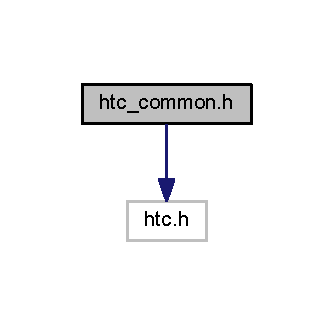
\includegraphics[width=160pt]{htc__common_8h__incl}
\end{center}
\end{figure}
\subsection*{Macros}
\begin{DoxyCompactItemize}
\item 
\#define {\bf R\-E\-G\-I\-S\-T\-E\-R\-\_\-\-T\-R\-I\-S\-A}~T\-R\-I\-S\-A
\item 
\#define {\bf R\-E\-G\-I\-S\-T\-E\-R\-\_\-\-T\-R\-I\-S\-B}~T\-R\-I\-S\-B
\item 
\#define {\bf R\-E\-G\-I\-S\-T\-E\-R\-\_\-\-T\-R\-I\-S\-C}~T\-R\-I\-S\-C
\item 
\#define {\bf R\-E\-G\-I\-S\-T\-E\-R\-\_\-\-T\-R\-I\-S\-D}~T\-R\-I\-S\-D
\item 
\#define {\bf R\-E\-G\-I\-S\-T\-E\-R\-\_\-\-T\-R\-I\-S\-E}~T\-R\-I\-S\-E
\item 
\#define {\bf R\-E\-G\-I\-S\-T\-E\-R\-\_\-\-P\-O\-R\-T\-A}~P\-O\-R\-T\-A
\item 
\#define {\bf R\-E\-G\-I\-S\-T\-E\-R\-\_\-\-P\-O\-R\-T\-A\-\_\-0}~R\-A0
\item 
\#define {\bf R\-E\-G\-I\-S\-T\-E\-R\-\_\-\-P\-O\-R\-T\-A\-\_\-1}~R\-A1
\item 
\#define {\bf R\-E\-G\-I\-S\-T\-E\-R\-\_\-\-P\-O\-R\-T\-A\-\_\-2}~R\-A2
\item 
\#define {\bf R\-E\-G\-I\-S\-T\-E\-R\-\_\-\-P\-O\-R\-T\-A\-\_\-3}~R\-A3
\item 
\#define {\bf R\-E\-G\-I\-S\-T\-E\-R\-\_\-\-P\-O\-R\-T\-A\-\_\-4}~R\-A4
\item 
\#define {\bf R\-E\-G\-I\-S\-T\-E\-R\-\_\-\-P\-O\-R\-T\-A\-\_\-5}~R\-A5
\item 
\#define {\bf R\-E\-G\-I\-S\-T\-E\-R\-\_\-\-P\-O\-R\-T\-A\-\_\-6}~R\-A6
\item 
\#define {\bf R\-E\-G\-I\-S\-T\-E\-R\-\_\-\-P\-O\-R\-T\-A\-\_\-7}~R\-A7
\item 
\#define {\bf R\-E\-G\-I\-S\-T\-E\-R\-\_\-\-P\-O\-R\-T\-B}~P\-O\-R\-T\-B
\item 
\#define {\bf R\-E\-G\-I\-S\-T\-E\-R\-\_\-\-P\-O\-R\-T\-B\-\_\-0}~R\-B0
\item 
\#define {\bf R\-E\-G\-I\-S\-T\-E\-R\-\_\-\-P\-O\-R\-T\-B\-\_\-1}~R\-B1
\item 
\#define {\bf R\-E\-G\-I\-S\-T\-E\-R\-\_\-\-P\-O\-R\-T\-B\-\_\-2}~R\-B2
\item 
\#define {\bf R\-E\-G\-I\-S\-T\-E\-R\-\_\-\-P\-O\-R\-T\-B\-\_\-3}~R\-B3
\item 
\#define {\bf R\-E\-G\-I\-S\-T\-E\-R\-\_\-\-P\-O\-R\-T\-B\-\_\-4}~R\-B4
\item 
\#define {\bf R\-E\-G\-I\-S\-T\-E\-R\-\_\-\-P\-O\-R\-T\-B\-\_\-5}~R\-B5
\item 
\#define {\bf R\-E\-G\-I\-S\-T\-E\-R\-\_\-\-P\-O\-R\-T\-B\-\_\-6}~R\-B6
\item 
\#define {\bf R\-E\-G\-I\-S\-T\-E\-R\-\_\-\-P\-O\-R\-T\-B\-\_\-7}~R\-B7
\item 
\#define {\bf R\-E\-G\-I\-S\-T\-E\-R\-\_\-\-P\-O\-R\-T\-C}~P\-O\-R\-T\-C
\item 
\#define {\bf R\-E\-G\-I\-S\-T\-E\-R\-\_\-\-P\-O\-R\-T\-C\-\_\-0}~R\-C0
\item 
\#define {\bf R\-E\-G\-I\-S\-T\-E\-R\-\_\-\-P\-O\-R\-T\-C\-\_\-1}~R\-C1
\item 
\#define {\bf R\-E\-G\-I\-S\-T\-E\-R\-\_\-\-P\-O\-R\-T\-C\-\_\-2}~R\-C2
\item 
\#define {\bf R\-E\-G\-I\-S\-T\-E\-R\-\_\-\-P\-O\-R\-T\-C\-\_\-3}~R\-C3
\item 
\#define {\bf R\-E\-G\-I\-S\-T\-E\-R\-\_\-\-P\-O\-R\-T\-C\-\_\-4}~R\-C4
\item 
\#define {\bf R\-E\-G\-I\-S\-T\-E\-R\-\_\-\-P\-O\-R\-T\-C\-\_\-5}~R\-C5
\item 
\#define {\bf R\-E\-G\-I\-S\-T\-E\-R\-\_\-\-P\-O\-R\-T\-C\-\_\-6}~R\-C6
\item 
\#define {\bf R\-E\-G\-I\-S\-T\-E\-R\-\_\-\-P\-O\-R\-T\-C\-\_\-7}~R\-C7
\item 
\#define {\bf R\-E\-G\-I\-S\-T\-E\-R\-\_\-\-P\-O\-R\-T\-D}~P\-O\-R\-T\-D
\item 
\#define {\bf R\-E\-G\-I\-S\-T\-E\-R\-\_\-\-P\-O\-R\-T\-D\-\_\-0}~R\-D0
\item 
\#define {\bf R\-E\-G\-I\-S\-T\-E\-R\-\_\-\-P\-O\-R\-T\-D\-\_\-1}~R\-D1
\item 
\#define {\bf R\-E\-G\-I\-S\-T\-E\-R\-\_\-\-P\-O\-R\-T\-D\-\_\-2}~R\-D2
\item 
\#define {\bf R\-E\-G\-I\-S\-T\-E\-R\-\_\-\-P\-O\-R\-T\-D\-\_\-3}~R\-D3
\item 
\#define {\bf R\-E\-G\-I\-S\-T\-E\-R\-\_\-\-P\-O\-R\-T\-D\-\_\-4}~R\-D4
\item 
\#define {\bf R\-E\-G\-I\-S\-T\-E\-R\-\_\-\-P\-O\-R\-T\-D\-\_\-5}~R\-D5
\item 
\#define {\bf R\-E\-G\-I\-S\-T\-E\-R\-\_\-\-P\-O\-R\-T\-D\-\_\-6}~R\-D6
\item 
\#define {\bf R\-E\-G\-I\-S\-T\-E\-R\-\_\-\-P\-O\-R\-T\-D\-\_\-7}~R\-D7
\item 
\#define {\bf R\-E\-G\-I\-S\-T\-E\-R\-\_\-\-P\-O\-R\-T\-E}~P\-O\-R\-T\-E
\item 
\#define {\bf R\-E\-G\-I\-S\-T\-E\-R\-\_\-\-P\-O\-R\-T\-E\-\_\-0}~R\-E0
\item 
\#define {\bf R\-E\-G\-I\-S\-T\-E\-R\-\_\-\-P\-O\-R\-T\-E\-\_\-1}~R\-E1
\item 
\#define {\bf R\-E\-G\-I\-S\-T\-E\-R\-\_\-\-P\-O\-R\-T\-E\-\_\-2}~R\-E2
\item 
\#define {\bf R\-E\-G\-I\-S\-T\-E\-R\-\_\-\-P\-O\-R\-T\-E\-\_\-3}~R\-E3
\item 
\#define {\bf R\-E\-G\-I\-S\-T\-E\-R\-\_\-\-P\-O\-R\-T\-E\-\_\-4}~R\-E4
\item 
\#define {\bf R\-E\-G\-I\-S\-T\-E\-R\-\_\-\-P\-O\-R\-T\-E\-\_\-5}~R\-E5
\item 
\#define {\bf R\-E\-G\-I\-S\-T\-E\-R\-\_\-\-P\-O\-R\-T\-E\-\_\-6}~R\-E6
\item 
\#define {\bf R\-E\-G\-I\-S\-T\-E\-R\-\_\-\-P\-O\-R\-T\-E\-\_\-7}~R\-E7
\item 
\#define {\bf R\-E\-G\-I\-S\-T\-E\-R\-\_\-\-T\-X\-R\-E\-G}~T\-X\-R\-E\-G
\item 
\#define {\bf R\-E\-G\-I\-S\-T\-E\-R\-\_\-\-R\-C\-R\-E\-G}~R\-C\-R\-E\-G
\item 
\#define {\bf R\-E\-G\-I\-S\-T\-E\-R\-\_\-\-S\-P\-B\-R\-G}~S\-P\-B\-R\-G
\item 
\#define {\bf R\-E\-G\-I\-S\-T\-E\-R\-\_\-\-T\-M\-R0\-H}~T\-M\-R0\-H
\item 
\#define {\bf R\-E\-G\-I\-S\-T\-E\-R\-\_\-\-T\-M\-R0\-L}~T\-M\-R0\-L
\item 
\#define {\bf R\-E\-G\-I\-S\-T\-E\-R\-\_\-\-T\-M\-R1\-H}~T\-M\-R1\-H
\item 
\#define {\bf R\-E\-G\-I\-S\-T\-E\-R\-\_\-\-T\-M\-R1\-L}~T\-M\-R1\-L
\item 
\#define {\bf R\-E\-G\-I\-S\-T\-E\-R\-\_\-\-T\-M\-R2\-H}~T\-M\-R2\-H
\item 
\#define {\bf R\-E\-G\-I\-S\-T\-E\-R\-\_\-\-T\-M\-R2\-L}~T\-M\-R2\-L
\item 
\#define {\bf R\-E\-G\-I\-S\-T\-E\-R\-\_\-\-A\-D\-R\-E\-S\-H}~A\-D\-R\-E\-S\-H
\item 
\#define {\bf R\-E\-G\-I\-S\-T\-E\-R\-\_\-\-A\-D\-R\-E\-S\-L}~A\-D\-R\-E\-S\-L
\end{DoxyCompactItemize}


\subsection{Macro Definition Documentation}
\index{htc\-\_\-common.\-h@{htc\-\_\-common.\-h}!R\-E\-G\-I\-S\-T\-E\-R\-\_\-\-A\-D\-R\-E\-S\-H@{R\-E\-G\-I\-S\-T\-E\-R\-\_\-\-A\-D\-R\-E\-S\-H}}
\index{R\-E\-G\-I\-S\-T\-E\-R\-\_\-\-A\-D\-R\-E\-S\-H@{R\-E\-G\-I\-S\-T\-E\-R\-\_\-\-A\-D\-R\-E\-S\-H}!htc_common.h@{htc\-\_\-common.\-h}}
\subsubsection[{R\-E\-G\-I\-S\-T\-E\-R\-\_\-\-A\-D\-R\-E\-S\-H}]{\setlength{\rightskip}{0pt plus 5cm}\#define R\-E\-G\-I\-S\-T\-E\-R\-\_\-\-A\-D\-R\-E\-S\-H~A\-D\-R\-E\-S\-H}\label{htc__common_8h_a756970e366df4d715b1345c874a29524}


Definition at line 105 of file htc\-\_\-common.\-h.

\index{htc\-\_\-common.\-h@{htc\-\_\-common.\-h}!R\-E\-G\-I\-S\-T\-E\-R\-\_\-\-A\-D\-R\-E\-S\-L@{R\-E\-G\-I\-S\-T\-E\-R\-\_\-\-A\-D\-R\-E\-S\-L}}
\index{R\-E\-G\-I\-S\-T\-E\-R\-\_\-\-A\-D\-R\-E\-S\-L@{R\-E\-G\-I\-S\-T\-E\-R\-\_\-\-A\-D\-R\-E\-S\-L}!htc_common.h@{htc\-\_\-common.\-h}}
\subsubsection[{R\-E\-G\-I\-S\-T\-E\-R\-\_\-\-A\-D\-R\-E\-S\-L}]{\setlength{\rightskip}{0pt plus 5cm}\#define R\-E\-G\-I\-S\-T\-E\-R\-\_\-\-A\-D\-R\-E\-S\-L~A\-D\-R\-E\-S\-L}\label{htc__common_8h_aa85a7d6de5a9c55ee50f5ee07a87920d}


Definition at line 106 of file htc\-\_\-common.\-h.

\index{htc\-\_\-common.\-h@{htc\-\_\-common.\-h}!R\-E\-G\-I\-S\-T\-E\-R\-\_\-\-P\-O\-R\-T\-A@{R\-E\-G\-I\-S\-T\-E\-R\-\_\-\-P\-O\-R\-T\-A}}
\index{R\-E\-G\-I\-S\-T\-E\-R\-\_\-\-P\-O\-R\-T\-A@{R\-E\-G\-I\-S\-T\-E\-R\-\_\-\-P\-O\-R\-T\-A}!htc_common.h@{htc\-\_\-common.\-h}}
\subsubsection[{R\-E\-G\-I\-S\-T\-E\-R\-\_\-\-P\-O\-R\-T\-A}]{\setlength{\rightskip}{0pt plus 5cm}\#define R\-E\-G\-I\-S\-T\-E\-R\-\_\-\-P\-O\-R\-T\-A~P\-O\-R\-T\-A}\label{htc__common_8h_a15d0f3b389dbb1d80657d115aae506e2}


Definition at line 42 of file htc\-\_\-common.\-h.

\index{htc\-\_\-common.\-h@{htc\-\_\-common.\-h}!R\-E\-G\-I\-S\-T\-E\-R\-\_\-\-P\-O\-R\-T\-A\-\_\-0@{R\-E\-G\-I\-S\-T\-E\-R\-\_\-\-P\-O\-R\-T\-A\-\_\-0}}
\index{R\-E\-G\-I\-S\-T\-E\-R\-\_\-\-P\-O\-R\-T\-A\-\_\-0@{R\-E\-G\-I\-S\-T\-E\-R\-\_\-\-P\-O\-R\-T\-A\-\_\-0}!htc_common.h@{htc\-\_\-common.\-h}}
\subsubsection[{R\-E\-G\-I\-S\-T\-E\-R\-\_\-\-P\-O\-R\-T\-A\-\_\-0}]{\setlength{\rightskip}{0pt plus 5cm}\#define R\-E\-G\-I\-S\-T\-E\-R\-\_\-\-P\-O\-R\-T\-A\-\_\-0~R\-A0}\label{htc__common_8h_aa97c4472fdd1869dcb27fb4694316336}


Definition at line 43 of file htc\-\_\-common.\-h.

\index{htc\-\_\-common.\-h@{htc\-\_\-common.\-h}!R\-E\-G\-I\-S\-T\-E\-R\-\_\-\-P\-O\-R\-T\-A\-\_\-1@{R\-E\-G\-I\-S\-T\-E\-R\-\_\-\-P\-O\-R\-T\-A\-\_\-1}}
\index{R\-E\-G\-I\-S\-T\-E\-R\-\_\-\-P\-O\-R\-T\-A\-\_\-1@{R\-E\-G\-I\-S\-T\-E\-R\-\_\-\-P\-O\-R\-T\-A\-\_\-1}!htc_common.h@{htc\-\_\-common.\-h}}
\subsubsection[{R\-E\-G\-I\-S\-T\-E\-R\-\_\-\-P\-O\-R\-T\-A\-\_\-1}]{\setlength{\rightskip}{0pt plus 5cm}\#define R\-E\-G\-I\-S\-T\-E\-R\-\_\-\-P\-O\-R\-T\-A\-\_\-1~R\-A1}\label{htc__common_8h_a931229c51d987a3d857c13fa27f5f2da}


Definition at line 44 of file htc\-\_\-common.\-h.

\index{htc\-\_\-common.\-h@{htc\-\_\-common.\-h}!R\-E\-G\-I\-S\-T\-E\-R\-\_\-\-P\-O\-R\-T\-A\-\_\-2@{R\-E\-G\-I\-S\-T\-E\-R\-\_\-\-P\-O\-R\-T\-A\-\_\-2}}
\index{R\-E\-G\-I\-S\-T\-E\-R\-\_\-\-P\-O\-R\-T\-A\-\_\-2@{R\-E\-G\-I\-S\-T\-E\-R\-\_\-\-P\-O\-R\-T\-A\-\_\-2}!htc_common.h@{htc\-\_\-common.\-h}}
\subsubsection[{R\-E\-G\-I\-S\-T\-E\-R\-\_\-\-P\-O\-R\-T\-A\-\_\-2}]{\setlength{\rightskip}{0pt plus 5cm}\#define R\-E\-G\-I\-S\-T\-E\-R\-\_\-\-P\-O\-R\-T\-A\-\_\-2~R\-A2}\label{htc__common_8h_a6480b050f7d3f30d04cfe35b98d8a36c}


Definition at line 45 of file htc\-\_\-common.\-h.

\index{htc\-\_\-common.\-h@{htc\-\_\-common.\-h}!R\-E\-G\-I\-S\-T\-E\-R\-\_\-\-P\-O\-R\-T\-A\-\_\-3@{R\-E\-G\-I\-S\-T\-E\-R\-\_\-\-P\-O\-R\-T\-A\-\_\-3}}
\index{R\-E\-G\-I\-S\-T\-E\-R\-\_\-\-P\-O\-R\-T\-A\-\_\-3@{R\-E\-G\-I\-S\-T\-E\-R\-\_\-\-P\-O\-R\-T\-A\-\_\-3}!htc_common.h@{htc\-\_\-common.\-h}}
\subsubsection[{R\-E\-G\-I\-S\-T\-E\-R\-\_\-\-P\-O\-R\-T\-A\-\_\-3}]{\setlength{\rightskip}{0pt plus 5cm}\#define R\-E\-G\-I\-S\-T\-E\-R\-\_\-\-P\-O\-R\-T\-A\-\_\-3~R\-A3}\label{htc__common_8h_ab4866699d5762371569d87fed19756c9}


Definition at line 46 of file htc\-\_\-common.\-h.

\index{htc\-\_\-common.\-h@{htc\-\_\-common.\-h}!R\-E\-G\-I\-S\-T\-E\-R\-\_\-\-P\-O\-R\-T\-A\-\_\-4@{R\-E\-G\-I\-S\-T\-E\-R\-\_\-\-P\-O\-R\-T\-A\-\_\-4}}
\index{R\-E\-G\-I\-S\-T\-E\-R\-\_\-\-P\-O\-R\-T\-A\-\_\-4@{R\-E\-G\-I\-S\-T\-E\-R\-\_\-\-P\-O\-R\-T\-A\-\_\-4}!htc_common.h@{htc\-\_\-common.\-h}}
\subsubsection[{R\-E\-G\-I\-S\-T\-E\-R\-\_\-\-P\-O\-R\-T\-A\-\_\-4}]{\setlength{\rightskip}{0pt plus 5cm}\#define R\-E\-G\-I\-S\-T\-E\-R\-\_\-\-P\-O\-R\-T\-A\-\_\-4~R\-A4}\label{htc__common_8h_ab223baf836d44fc42dd3a091b32a5c18}


Definition at line 47 of file htc\-\_\-common.\-h.

\index{htc\-\_\-common.\-h@{htc\-\_\-common.\-h}!R\-E\-G\-I\-S\-T\-E\-R\-\_\-\-P\-O\-R\-T\-A\-\_\-5@{R\-E\-G\-I\-S\-T\-E\-R\-\_\-\-P\-O\-R\-T\-A\-\_\-5}}
\index{R\-E\-G\-I\-S\-T\-E\-R\-\_\-\-P\-O\-R\-T\-A\-\_\-5@{R\-E\-G\-I\-S\-T\-E\-R\-\_\-\-P\-O\-R\-T\-A\-\_\-5}!htc_common.h@{htc\-\_\-common.\-h}}
\subsubsection[{R\-E\-G\-I\-S\-T\-E\-R\-\_\-\-P\-O\-R\-T\-A\-\_\-5}]{\setlength{\rightskip}{0pt plus 5cm}\#define R\-E\-G\-I\-S\-T\-E\-R\-\_\-\-P\-O\-R\-T\-A\-\_\-5~R\-A5}\label{htc__common_8h_ae2e4db386a4e5f8d088cfd78e5db9c98}


Definition at line 48 of file htc\-\_\-common.\-h.

\index{htc\-\_\-common.\-h@{htc\-\_\-common.\-h}!R\-E\-G\-I\-S\-T\-E\-R\-\_\-\-P\-O\-R\-T\-A\-\_\-6@{R\-E\-G\-I\-S\-T\-E\-R\-\_\-\-P\-O\-R\-T\-A\-\_\-6}}
\index{R\-E\-G\-I\-S\-T\-E\-R\-\_\-\-P\-O\-R\-T\-A\-\_\-6@{R\-E\-G\-I\-S\-T\-E\-R\-\_\-\-P\-O\-R\-T\-A\-\_\-6}!htc_common.h@{htc\-\_\-common.\-h}}
\subsubsection[{R\-E\-G\-I\-S\-T\-E\-R\-\_\-\-P\-O\-R\-T\-A\-\_\-6}]{\setlength{\rightskip}{0pt plus 5cm}\#define R\-E\-G\-I\-S\-T\-E\-R\-\_\-\-P\-O\-R\-T\-A\-\_\-6~R\-A6}\label{htc__common_8h_a2f289415c848f86f0f5252f76a7754bc}


Definition at line 49 of file htc\-\_\-common.\-h.

\index{htc\-\_\-common.\-h@{htc\-\_\-common.\-h}!R\-E\-G\-I\-S\-T\-E\-R\-\_\-\-P\-O\-R\-T\-A\-\_\-7@{R\-E\-G\-I\-S\-T\-E\-R\-\_\-\-P\-O\-R\-T\-A\-\_\-7}}
\index{R\-E\-G\-I\-S\-T\-E\-R\-\_\-\-P\-O\-R\-T\-A\-\_\-7@{R\-E\-G\-I\-S\-T\-E\-R\-\_\-\-P\-O\-R\-T\-A\-\_\-7}!htc_common.h@{htc\-\_\-common.\-h}}
\subsubsection[{R\-E\-G\-I\-S\-T\-E\-R\-\_\-\-P\-O\-R\-T\-A\-\_\-7}]{\setlength{\rightskip}{0pt plus 5cm}\#define R\-E\-G\-I\-S\-T\-E\-R\-\_\-\-P\-O\-R\-T\-A\-\_\-7~R\-A7}\label{htc__common_8h_ac0459c6fe2c73376bc7466b8749bdab1}


Definition at line 50 of file htc\-\_\-common.\-h.

\index{htc\-\_\-common.\-h@{htc\-\_\-common.\-h}!R\-E\-G\-I\-S\-T\-E\-R\-\_\-\-P\-O\-R\-T\-B@{R\-E\-G\-I\-S\-T\-E\-R\-\_\-\-P\-O\-R\-T\-B}}
\index{R\-E\-G\-I\-S\-T\-E\-R\-\_\-\-P\-O\-R\-T\-B@{R\-E\-G\-I\-S\-T\-E\-R\-\_\-\-P\-O\-R\-T\-B}!htc_common.h@{htc\-\_\-common.\-h}}
\subsubsection[{R\-E\-G\-I\-S\-T\-E\-R\-\_\-\-P\-O\-R\-T\-B}]{\setlength{\rightskip}{0pt plus 5cm}\#define R\-E\-G\-I\-S\-T\-E\-R\-\_\-\-P\-O\-R\-T\-B~P\-O\-R\-T\-B}\label{htc__common_8h_ae1fec3d60f2e07c64360cb468bf16366}


Definition at line 52 of file htc\-\_\-common.\-h.

\index{htc\-\_\-common.\-h@{htc\-\_\-common.\-h}!R\-E\-G\-I\-S\-T\-E\-R\-\_\-\-P\-O\-R\-T\-B\-\_\-0@{R\-E\-G\-I\-S\-T\-E\-R\-\_\-\-P\-O\-R\-T\-B\-\_\-0}}
\index{R\-E\-G\-I\-S\-T\-E\-R\-\_\-\-P\-O\-R\-T\-B\-\_\-0@{R\-E\-G\-I\-S\-T\-E\-R\-\_\-\-P\-O\-R\-T\-B\-\_\-0}!htc_common.h@{htc\-\_\-common.\-h}}
\subsubsection[{R\-E\-G\-I\-S\-T\-E\-R\-\_\-\-P\-O\-R\-T\-B\-\_\-0}]{\setlength{\rightskip}{0pt plus 5cm}\#define R\-E\-G\-I\-S\-T\-E\-R\-\_\-\-P\-O\-R\-T\-B\-\_\-0~R\-B0}\label{htc__common_8h_aa555878ed2dc77ecb5fc06ac553a27d8}


Definition at line 53 of file htc\-\_\-common.\-h.

\index{htc\-\_\-common.\-h@{htc\-\_\-common.\-h}!R\-E\-G\-I\-S\-T\-E\-R\-\_\-\-P\-O\-R\-T\-B\-\_\-1@{R\-E\-G\-I\-S\-T\-E\-R\-\_\-\-P\-O\-R\-T\-B\-\_\-1}}
\index{R\-E\-G\-I\-S\-T\-E\-R\-\_\-\-P\-O\-R\-T\-B\-\_\-1@{R\-E\-G\-I\-S\-T\-E\-R\-\_\-\-P\-O\-R\-T\-B\-\_\-1}!htc_common.h@{htc\-\_\-common.\-h}}
\subsubsection[{R\-E\-G\-I\-S\-T\-E\-R\-\_\-\-P\-O\-R\-T\-B\-\_\-1}]{\setlength{\rightskip}{0pt plus 5cm}\#define R\-E\-G\-I\-S\-T\-E\-R\-\_\-\-P\-O\-R\-T\-B\-\_\-1~R\-B1}\label{htc__common_8h_af4989a8173869bf110114256e2241aad}


Definition at line 54 of file htc\-\_\-common.\-h.

\index{htc\-\_\-common.\-h@{htc\-\_\-common.\-h}!R\-E\-G\-I\-S\-T\-E\-R\-\_\-\-P\-O\-R\-T\-B\-\_\-2@{R\-E\-G\-I\-S\-T\-E\-R\-\_\-\-P\-O\-R\-T\-B\-\_\-2}}
\index{R\-E\-G\-I\-S\-T\-E\-R\-\_\-\-P\-O\-R\-T\-B\-\_\-2@{R\-E\-G\-I\-S\-T\-E\-R\-\_\-\-P\-O\-R\-T\-B\-\_\-2}!htc_common.h@{htc\-\_\-common.\-h}}
\subsubsection[{R\-E\-G\-I\-S\-T\-E\-R\-\_\-\-P\-O\-R\-T\-B\-\_\-2}]{\setlength{\rightskip}{0pt plus 5cm}\#define R\-E\-G\-I\-S\-T\-E\-R\-\_\-\-P\-O\-R\-T\-B\-\_\-2~R\-B2}\label{htc__common_8h_a3fe067c85b09edfe8097abfc0345deaa}


Definition at line 55 of file htc\-\_\-common.\-h.

\index{htc\-\_\-common.\-h@{htc\-\_\-common.\-h}!R\-E\-G\-I\-S\-T\-E\-R\-\_\-\-P\-O\-R\-T\-B\-\_\-3@{R\-E\-G\-I\-S\-T\-E\-R\-\_\-\-P\-O\-R\-T\-B\-\_\-3}}
\index{R\-E\-G\-I\-S\-T\-E\-R\-\_\-\-P\-O\-R\-T\-B\-\_\-3@{R\-E\-G\-I\-S\-T\-E\-R\-\_\-\-P\-O\-R\-T\-B\-\_\-3}!htc_common.h@{htc\-\_\-common.\-h}}
\subsubsection[{R\-E\-G\-I\-S\-T\-E\-R\-\_\-\-P\-O\-R\-T\-B\-\_\-3}]{\setlength{\rightskip}{0pt plus 5cm}\#define R\-E\-G\-I\-S\-T\-E\-R\-\_\-\-P\-O\-R\-T\-B\-\_\-3~R\-B3}\label{htc__common_8h_a835112043463971ce9b56999c2739cdf}


Definition at line 56 of file htc\-\_\-common.\-h.

\index{htc\-\_\-common.\-h@{htc\-\_\-common.\-h}!R\-E\-G\-I\-S\-T\-E\-R\-\_\-\-P\-O\-R\-T\-B\-\_\-4@{R\-E\-G\-I\-S\-T\-E\-R\-\_\-\-P\-O\-R\-T\-B\-\_\-4}}
\index{R\-E\-G\-I\-S\-T\-E\-R\-\_\-\-P\-O\-R\-T\-B\-\_\-4@{R\-E\-G\-I\-S\-T\-E\-R\-\_\-\-P\-O\-R\-T\-B\-\_\-4}!htc_common.h@{htc\-\_\-common.\-h}}
\subsubsection[{R\-E\-G\-I\-S\-T\-E\-R\-\_\-\-P\-O\-R\-T\-B\-\_\-4}]{\setlength{\rightskip}{0pt plus 5cm}\#define R\-E\-G\-I\-S\-T\-E\-R\-\_\-\-P\-O\-R\-T\-B\-\_\-4~R\-B4}\label{htc__common_8h_a2a899d0d8ba646fcb9a4afb009cef4cb}


Definition at line 57 of file htc\-\_\-common.\-h.

\index{htc\-\_\-common.\-h@{htc\-\_\-common.\-h}!R\-E\-G\-I\-S\-T\-E\-R\-\_\-\-P\-O\-R\-T\-B\-\_\-5@{R\-E\-G\-I\-S\-T\-E\-R\-\_\-\-P\-O\-R\-T\-B\-\_\-5}}
\index{R\-E\-G\-I\-S\-T\-E\-R\-\_\-\-P\-O\-R\-T\-B\-\_\-5@{R\-E\-G\-I\-S\-T\-E\-R\-\_\-\-P\-O\-R\-T\-B\-\_\-5}!htc_common.h@{htc\-\_\-common.\-h}}
\subsubsection[{R\-E\-G\-I\-S\-T\-E\-R\-\_\-\-P\-O\-R\-T\-B\-\_\-5}]{\setlength{\rightskip}{0pt plus 5cm}\#define R\-E\-G\-I\-S\-T\-E\-R\-\_\-\-P\-O\-R\-T\-B\-\_\-5~R\-B5}\label{htc__common_8h_abde28842d7c649683c916a8169932b89}


Definition at line 58 of file htc\-\_\-common.\-h.

\index{htc\-\_\-common.\-h@{htc\-\_\-common.\-h}!R\-E\-G\-I\-S\-T\-E\-R\-\_\-\-P\-O\-R\-T\-B\-\_\-6@{R\-E\-G\-I\-S\-T\-E\-R\-\_\-\-P\-O\-R\-T\-B\-\_\-6}}
\index{R\-E\-G\-I\-S\-T\-E\-R\-\_\-\-P\-O\-R\-T\-B\-\_\-6@{R\-E\-G\-I\-S\-T\-E\-R\-\_\-\-P\-O\-R\-T\-B\-\_\-6}!htc_common.h@{htc\-\_\-common.\-h}}
\subsubsection[{R\-E\-G\-I\-S\-T\-E\-R\-\_\-\-P\-O\-R\-T\-B\-\_\-6}]{\setlength{\rightskip}{0pt plus 5cm}\#define R\-E\-G\-I\-S\-T\-E\-R\-\_\-\-P\-O\-R\-T\-B\-\_\-6~R\-B6}\label{htc__common_8h_acfbb9d8a2c4e9b9f31f397394df752db}


Definition at line 59 of file htc\-\_\-common.\-h.

\index{htc\-\_\-common.\-h@{htc\-\_\-common.\-h}!R\-E\-G\-I\-S\-T\-E\-R\-\_\-\-P\-O\-R\-T\-B\-\_\-7@{R\-E\-G\-I\-S\-T\-E\-R\-\_\-\-P\-O\-R\-T\-B\-\_\-7}}
\index{R\-E\-G\-I\-S\-T\-E\-R\-\_\-\-P\-O\-R\-T\-B\-\_\-7@{R\-E\-G\-I\-S\-T\-E\-R\-\_\-\-P\-O\-R\-T\-B\-\_\-7}!htc_common.h@{htc\-\_\-common.\-h}}
\subsubsection[{R\-E\-G\-I\-S\-T\-E\-R\-\_\-\-P\-O\-R\-T\-B\-\_\-7}]{\setlength{\rightskip}{0pt plus 5cm}\#define R\-E\-G\-I\-S\-T\-E\-R\-\_\-\-P\-O\-R\-T\-B\-\_\-7~R\-B7}\label{htc__common_8h_a37c7e8e9ba7af61ed29f1ce1e42c64cc}


Definition at line 60 of file htc\-\_\-common.\-h.

\index{htc\-\_\-common.\-h@{htc\-\_\-common.\-h}!R\-E\-G\-I\-S\-T\-E\-R\-\_\-\-P\-O\-R\-T\-C@{R\-E\-G\-I\-S\-T\-E\-R\-\_\-\-P\-O\-R\-T\-C}}
\index{R\-E\-G\-I\-S\-T\-E\-R\-\_\-\-P\-O\-R\-T\-C@{R\-E\-G\-I\-S\-T\-E\-R\-\_\-\-P\-O\-R\-T\-C}!htc_common.h@{htc\-\_\-common.\-h}}
\subsubsection[{R\-E\-G\-I\-S\-T\-E\-R\-\_\-\-P\-O\-R\-T\-C}]{\setlength{\rightskip}{0pt plus 5cm}\#define R\-E\-G\-I\-S\-T\-E\-R\-\_\-\-P\-O\-R\-T\-C~P\-O\-R\-T\-C}\label{htc__common_8h_a5c3107e516cc5b978f44eae861a67976}


Definition at line 62 of file htc\-\_\-common.\-h.

\index{htc\-\_\-common.\-h@{htc\-\_\-common.\-h}!R\-E\-G\-I\-S\-T\-E\-R\-\_\-\-P\-O\-R\-T\-C\-\_\-0@{R\-E\-G\-I\-S\-T\-E\-R\-\_\-\-P\-O\-R\-T\-C\-\_\-0}}
\index{R\-E\-G\-I\-S\-T\-E\-R\-\_\-\-P\-O\-R\-T\-C\-\_\-0@{R\-E\-G\-I\-S\-T\-E\-R\-\_\-\-P\-O\-R\-T\-C\-\_\-0}!htc_common.h@{htc\-\_\-common.\-h}}
\subsubsection[{R\-E\-G\-I\-S\-T\-E\-R\-\_\-\-P\-O\-R\-T\-C\-\_\-0}]{\setlength{\rightskip}{0pt plus 5cm}\#define R\-E\-G\-I\-S\-T\-E\-R\-\_\-\-P\-O\-R\-T\-C\-\_\-0~R\-C0}\label{htc__common_8h_a71cfeb870b3b15d5d4ab408c1b7f4e19}


Definition at line 63 of file htc\-\_\-common.\-h.

\index{htc\-\_\-common.\-h@{htc\-\_\-common.\-h}!R\-E\-G\-I\-S\-T\-E\-R\-\_\-\-P\-O\-R\-T\-C\-\_\-1@{R\-E\-G\-I\-S\-T\-E\-R\-\_\-\-P\-O\-R\-T\-C\-\_\-1}}
\index{R\-E\-G\-I\-S\-T\-E\-R\-\_\-\-P\-O\-R\-T\-C\-\_\-1@{R\-E\-G\-I\-S\-T\-E\-R\-\_\-\-P\-O\-R\-T\-C\-\_\-1}!htc_common.h@{htc\-\_\-common.\-h}}
\subsubsection[{R\-E\-G\-I\-S\-T\-E\-R\-\_\-\-P\-O\-R\-T\-C\-\_\-1}]{\setlength{\rightskip}{0pt plus 5cm}\#define R\-E\-G\-I\-S\-T\-E\-R\-\_\-\-P\-O\-R\-T\-C\-\_\-1~R\-C1}\label{htc__common_8h_a943ec7ed293fb4b7109e1d0160c0d938}


Definition at line 64 of file htc\-\_\-common.\-h.

\index{htc\-\_\-common.\-h@{htc\-\_\-common.\-h}!R\-E\-G\-I\-S\-T\-E\-R\-\_\-\-P\-O\-R\-T\-C\-\_\-2@{R\-E\-G\-I\-S\-T\-E\-R\-\_\-\-P\-O\-R\-T\-C\-\_\-2}}
\index{R\-E\-G\-I\-S\-T\-E\-R\-\_\-\-P\-O\-R\-T\-C\-\_\-2@{R\-E\-G\-I\-S\-T\-E\-R\-\_\-\-P\-O\-R\-T\-C\-\_\-2}!htc_common.h@{htc\-\_\-common.\-h}}
\subsubsection[{R\-E\-G\-I\-S\-T\-E\-R\-\_\-\-P\-O\-R\-T\-C\-\_\-2}]{\setlength{\rightskip}{0pt plus 5cm}\#define R\-E\-G\-I\-S\-T\-E\-R\-\_\-\-P\-O\-R\-T\-C\-\_\-2~R\-C2}\label{htc__common_8h_ad11a21ae016e9e4f25114c16432f1f4f}


Definition at line 65 of file htc\-\_\-common.\-h.

\index{htc\-\_\-common.\-h@{htc\-\_\-common.\-h}!R\-E\-G\-I\-S\-T\-E\-R\-\_\-\-P\-O\-R\-T\-C\-\_\-3@{R\-E\-G\-I\-S\-T\-E\-R\-\_\-\-P\-O\-R\-T\-C\-\_\-3}}
\index{R\-E\-G\-I\-S\-T\-E\-R\-\_\-\-P\-O\-R\-T\-C\-\_\-3@{R\-E\-G\-I\-S\-T\-E\-R\-\_\-\-P\-O\-R\-T\-C\-\_\-3}!htc_common.h@{htc\-\_\-common.\-h}}
\subsubsection[{R\-E\-G\-I\-S\-T\-E\-R\-\_\-\-P\-O\-R\-T\-C\-\_\-3}]{\setlength{\rightskip}{0pt plus 5cm}\#define R\-E\-G\-I\-S\-T\-E\-R\-\_\-\-P\-O\-R\-T\-C\-\_\-3~R\-C3}\label{htc__common_8h_a6c36932c3c945aca796b2d2ccbba4069}


Definition at line 66 of file htc\-\_\-common.\-h.

\index{htc\-\_\-common.\-h@{htc\-\_\-common.\-h}!R\-E\-G\-I\-S\-T\-E\-R\-\_\-\-P\-O\-R\-T\-C\-\_\-4@{R\-E\-G\-I\-S\-T\-E\-R\-\_\-\-P\-O\-R\-T\-C\-\_\-4}}
\index{R\-E\-G\-I\-S\-T\-E\-R\-\_\-\-P\-O\-R\-T\-C\-\_\-4@{R\-E\-G\-I\-S\-T\-E\-R\-\_\-\-P\-O\-R\-T\-C\-\_\-4}!htc_common.h@{htc\-\_\-common.\-h}}
\subsubsection[{R\-E\-G\-I\-S\-T\-E\-R\-\_\-\-P\-O\-R\-T\-C\-\_\-4}]{\setlength{\rightskip}{0pt plus 5cm}\#define R\-E\-G\-I\-S\-T\-E\-R\-\_\-\-P\-O\-R\-T\-C\-\_\-4~R\-C4}\label{htc__common_8h_a377603a9b36b5bfac788805471bc3ad0}


Definition at line 67 of file htc\-\_\-common.\-h.

\index{htc\-\_\-common.\-h@{htc\-\_\-common.\-h}!R\-E\-G\-I\-S\-T\-E\-R\-\_\-\-P\-O\-R\-T\-C\-\_\-5@{R\-E\-G\-I\-S\-T\-E\-R\-\_\-\-P\-O\-R\-T\-C\-\_\-5}}
\index{R\-E\-G\-I\-S\-T\-E\-R\-\_\-\-P\-O\-R\-T\-C\-\_\-5@{R\-E\-G\-I\-S\-T\-E\-R\-\_\-\-P\-O\-R\-T\-C\-\_\-5}!htc_common.h@{htc\-\_\-common.\-h}}
\subsubsection[{R\-E\-G\-I\-S\-T\-E\-R\-\_\-\-P\-O\-R\-T\-C\-\_\-5}]{\setlength{\rightskip}{0pt plus 5cm}\#define R\-E\-G\-I\-S\-T\-E\-R\-\_\-\-P\-O\-R\-T\-C\-\_\-5~R\-C5}\label{htc__common_8h_a5db3cf9404404fcb18da5c7d766a02a5}


Definition at line 68 of file htc\-\_\-common.\-h.

\index{htc\-\_\-common.\-h@{htc\-\_\-common.\-h}!R\-E\-G\-I\-S\-T\-E\-R\-\_\-\-P\-O\-R\-T\-C\-\_\-6@{R\-E\-G\-I\-S\-T\-E\-R\-\_\-\-P\-O\-R\-T\-C\-\_\-6}}
\index{R\-E\-G\-I\-S\-T\-E\-R\-\_\-\-P\-O\-R\-T\-C\-\_\-6@{R\-E\-G\-I\-S\-T\-E\-R\-\_\-\-P\-O\-R\-T\-C\-\_\-6}!htc_common.h@{htc\-\_\-common.\-h}}
\subsubsection[{R\-E\-G\-I\-S\-T\-E\-R\-\_\-\-P\-O\-R\-T\-C\-\_\-6}]{\setlength{\rightskip}{0pt plus 5cm}\#define R\-E\-G\-I\-S\-T\-E\-R\-\_\-\-P\-O\-R\-T\-C\-\_\-6~R\-C6}\label{htc__common_8h_a00b736712f8eea867e873e6e298f3ad3}


Definition at line 69 of file htc\-\_\-common.\-h.

\index{htc\-\_\-common.\-h@{htc\-\_\-common.\-h}!R\-E\-G\-I\-S\-T\-E\-R\-\_\-\-P\-O\-R\-T\-C\-\_\-7@{R\-E\-G\-I\-S\-T\-E\-R\-\_\-\-P\-O\-R\-T\-C\-\_\-7}}
\index{R\-E\-G\-I\-S\-T\-E\-R\-\_\-\-P\-O\-R\-T\-C\-\_\-7@{R\-E\-G\-I\-S\-T\-E\-R\-\_\-\-P\-O\-R\-T\-C\-\_\-7}!htc_common.h@{htc\-\_\-common.\-h}}
\subsubsection[{R\-E\-G\-I\-S\-T\-E\-R\-\_\-\-P\-O\-R\-T\-C\-\_\-7}]{\setlength{\rightskip}{0pt plus 5cm}\#define R\-E\-G\-I\-S\-T\-E\-R\-\_\-\-P\-O\-R\-T\-C\-\_\-7~R\-C7}\label{htc__common_8h_a5a2b4128fc146904baddea920269f0a7}


Definition at line 70 of file htc\-\_\-common.\-h.

\index{htc\-\_\-common.\-h@{htc\-\_\-common.\-h}!R\-E\-G\-I\-S\-T\-E\-R\-\_\-\-P\-O\-R\-T\-D@{R\-E\-G\-I\-S\-T\-E\-R\-\_\-\-P\-O\-R\-T\-D}}
\index{R\-E\-G\-I\-S\-T\-E\-R\-\_\-\-P\-O\-R\-T\-D@{R\-E\-G\-I\-S\-T\-E\-R\-\_\-\-P\-O\-R\-T\-D}!htc_common.h@{htc\-\_\-common.\-h}}
\subsubsection[{R\-E\-G\-I\-S\-T\-E\-R\-\_\-\-P\-O\-R\-T\-D}]{\setlength{\rightskip}{0pt plus 5cm}\#define R\-E\-G\-I\-S\-T\-E\-R\-\_\-\-P\-O\-R\-T\-D~P\-O\-R\-T\-D}\label{htc__common_8h_ad70a1196e5ce6d4fe1fd2c70c2f9be8e}


Definition at line 72 of file htc\-\_\-common.\-h.

\index{htc\-\_\-common.\-h@{htc\-\_\-common.\-h}!R\-E\-G\-I\-S\-T\-E\-R\-\_\-\-P\-O\-R\-T\-D\-\_\-0@{R\-E\-G\-I\-S\-T\-E\-R\-\_\-\-P\-O\-R\-T\-D\-\_\-0}}
\index{R\-E\-G\-I\-S\-T\-E\-R\-\_\-\-P\-O\-R\-T\-D\-\_\-0@{R\-E\-G\-I\-S\-T\-E\-R\-\_\-\-P\-O\-R\-T\-D\-\_\-0}!htc_common.h@{htc\-\_\-common.\-h}}
\subsubsection[{R\-E\-G\-I\-S\-T\-E\-R\-\_\-\-P\-O\-R\-T\-D\-\_\-0}]{\setlength{\rightskip}{0pt plus 5cm}\#define R\-E\-G\-I\-S\-T\-E\-R\-\_\-\-P\-O\-R\-T\-D\-\_\-0~R\-D0}\label{htc__common_8h_a4e337c2850dbcda76ad43752921a8da8}


Definition at line 73 of file htc\-\_\-common.\-h.

\index{htc\-\_\-common.\-h@{htc\-\_\-common.\-h}!R\-E\-G\-I\-S\-T\-E\-R\-\_\-\-P\-O\-R\-T\-D\-\_\-1@{R\-E\-G\-I\-S\-T\-E\-R\-\_\-\-P\-O\-R\-T\-D\-\_\-1}}
\index{R\-E\-G\-I\-S\-T\-E\-R\-\_\-\-P\-O\-R\-T\-D\-\_\-1@{R\-E\-G\-I\-S\-T\-E\-R\-\_\-\-P\-O\-R\-T\-D\-\_\-1}!htc_common.h@{htc\-\_\-common.\-h}}
\subsubsection[{R\-E\-G\-I\-S\-T\-E\-R\-\_\-\-P\-O\-R\-T\-D\-\_\-1}]{\setlength{\rightskip}{0pt plus 5cm}\#define R\-E\-G\-I\-S\-T\-E\-R\-\_\-\-P\-O\-R\-T\-D\-\_\-1~R\-D1}\label{htc__common_8h_a2d9c040e92f2b8278c596aed85f9062a}


Definition at line 74 of file htc\-\_\-common.\-h.

\index{htc\-\_\-common.\-h@{htc\-\_\-common.\-h}!R\-E\-G\-I\-S\-T\-E\-R\-\_\-\-P\-O\-R\-T\-D\-\_\-2@{R\-E\-G\-I\-S\-T\-E\-R\-\_\-\-P\-O\-R\-T\-D\-\_\-2}}
\index{R\-E\-G\-I\-S\-T\-E\-R\-\_\-\-P\-O\-R\-T\-D\-\_\-2@{R\-E\-G\-I\-S\-T\-E\-R\-\_\-\-P\-O\-R\-T\-D\-\_\-2}!htc_common.h@{htc\-\_\-common.\-h}}
\subsubsection[{R\-E\-G\-I\-S\-T\-E\-R\-\_\-\-P\-O\-R\-T\-D\-\_\-2}]{\setlength{\rightskip}{0pt plus 5cm}\#define R\-E\-G\-I\-S\-T\-E\-R\-\_\-\-P\-O\-R\-T\-D\-\_\-2~R\-D2}\label{htc__common_8h_ad5c53a55902febf96730aa2e3686f3a5}


Definition at line 75 of file htc\-\_\-common.\-h.

\index{htc\-\_\-common.\-h@{htc\-\_\-common.\-h}!R\-E\-G\-I\-S\-T\-E\-R\-\_\-\-P\-O\-R\-T\-D\-\_\-3@{R\-E\-G\-I\-S\-T\-E\-R\-\_\-\-P\-O\-R\-T\-D\-\_\-3}}
\index{R\-E\-G\-I\-S\-T\-E\-R\-\_\-\-P\-O\-R\-T\-D\-\_\-3@{R\-E\-G\-I\-S\-T\-E\-R\-\_\-\-P\-O\-R\-T\-D\-\_\-3}!htc_common.h@{htc\-\_\-common.\-h}}
\subsubsection[{R\-E\-G\-I\-S\-T\-E\-R\-\_\-\-P\-O\-R\-T\-D\-\_\-3}]{\setlength{\rightskip}{0pt plus 5cm}\#define R\-E\-G\-I\-S\-T\-E\-R\-\_\-\-P\-O\-R\-T\-D\-\_\-3~R\-D3}\label{htc__common_8h_a1c664237fda2c821886e0b1292f82305}


Definition at line 76 of file htc\-\_\-common.\-h.

\index{htc\-\_\-common.\-h@{htc\-\_\-common.\-h}!R\-E\-G\-I\-S\-T\-E\-R\-\_\-\-P\-O\-R\-T\-D\-\_\-4@{R\-E\-G\-I\-S\-T\-E\-R\-\_\-\-P\-O\-R\-T\-D\-\_\-4}}
\index{R\-E\-G\-I\-S\-T\-E\-R\-\_\-\-P\-O\-R\-T\-D\-\_\-4@{R\-E\-G\-I\-S\-T\-E\-R\-\_\-\-P\-O\-R\-T\-D\-\_\-4}!htc_common.h@{htc\-\_\-common.\-h}}
\subsubsection[{R\-E\-G\-I\-S\-T\-E\-R\-\_\-\-P\-O\-R\-T\-D\-\_\-4}]{\setlength{\rightskip}{0pt plus 5cm}\#define R\-E\-G\-I\-S\-T\-E\-R\-\_\-\-P\-O\-R\-T\-D\-\_\-4~R\-D4}\label{htc__common_8h_a87655b068d9eb03aaa963a19aa51d103}


Definition at line 77 of file htc\-\_\-common.\-h.

\index{htc\-\_\-common.\-h@{htc\-\_\-common.\-h}!R\-E\-G\-I\-S\-T\-E\-R\-\_\-\-P\-O\-R\-T\-D\-\_\-5@{R\-E\-G\-I\-S\-T\-E\-R\-\_\-\-P\-O\-R\-T\-D\-\_\-5}}
\index{R\-E\-G\-I\-S\-T\-E\-R\-\_\-\-P\-O\-R\-T\-D\-\_\-5@{R\-E\-G\-I\-S\-T\-E\-R\-\_\-\-P\-O\-R\-T\-D\-\_\-5}!htc_common.h@{htc\-\_\-common.\-h}}
\subsubsection[{R\-E\-G\-I\-S\-T\-E\-R\-\_\-\-P\-O\-R\-T\-D\-\_\-5}]{\setlength{\rightskip}{0pt plus 5cm}\#define R\-E\-G\-I\-S\-T\-E\-R\-\_\-\-P\-O\-R\-T\-D\-\_\-5~R\-D5}\label{htc__common_8h_a563a1bcb196b72295e6d8cce66cd3e38}


Definition at line 78 of file htc\-\_\-common.\-h.

\index{htc\-\_\-common.\-h@{htc\-\_\-common.\-h}!R\-E\-G\-I\-S\-T\-E\-R\-\_\-\-P\-O\-R\-T\-D\-\_\-6@{R\-E\-G\-I\-S\-T\-E\-R\-\_\-\-P\-O\-R\-T\-D\-\_\-6}}
\index{R\-E\-G\-I\-S\-T\-E\-R\-\_\-\-P\-O\-R\-T\-D\-\_\-6@{R\-E\-G\-I\-S\-T\-E\-R\-\_\-\-P\-O\-R\-T\-D\-\_\-6}!htc_common.h@{htc\-\_\-common.\-h}}
\subsubsection[{R\-E\-G\-I\-S\-T\-E\-R\-\_\-\-P\-O\-R\-T\-D\-\_\-6}]{\setlength{\rightskip}{0pt plus 5cm}\#define R\-E\-G\-I\-S\-T\-E\-R\-\_\-\-P\-O\-R\-T\-D\-\_\-6~R\-D6}\label{htc__common_8h_a3a8ed605d2b7bf9bde1ed44f8c91a302}


Definition at line 79 of file htc\-\_\-common.\-h.

\index{htc\-\_\-common.\-h@{htc\-\_\-common.\-h}!R\-E\-G\-I\-S\-T\-E\-R\-\_\-\-P\-O\-R\-T\-D\-\_\-7@{R\-E\-G\-I\-S\-T\-E\-R\-\_\-\-P\-O\-R\-T\-D\-\_\-7}}
\index{R\-E\-G\-I\-S\-T\-E\-R\-\_\-\-P\-O\-R\-T\-D\-\_\-7@{R\-E\-G\-I\-S\-T\-E\-R\-\_\-\-P\-O\-R\-T\-D\-\_\-7}!htc_common.h@{htc\-\_\-common.\-h}}
\subsubsection[{R\-E\-G\-I\-S\-T\-E\-R\-\_\-\-P\-O\-R\-T\-D\-\_\-7}]{\setlength{\rightskip}{0pt plus 5cm}\#define R\-E\-G\-I\-S\-T\-E\-R\-\_\-\-P\-O\-R\-T\-D\-\_\-7~R\-D7}\label{htc__common_8h_ab75707fa9fbb8685f4aaf4b483294997}


Definition at line 80 of file htc\-\_\-common.\-h.

\index{htc\-\_\-common.\-h@{htc\-\_\-common.\-h}!R\-E\-G\-I\-S\-T\-E\-R\-\_\-\-P\-O\-R\-T\-E@{R\-E\-G\-I\-S\-T\-E\-R\-\_\-\-P\-O\-R\-T\-E}}
\index{R\-E\-G\-I\-S\-T\-E\-R\-\_\-\-P\-O\-R\-T\-E@{R\-E\-G\-I\-S\-T\-E\-R\-\_\-\-P\-O\-R\-T\-E}!htc_common.h@{htc\-\_\-common.\-h}}
\subsubsection[{R\-E\-G\-I\-S\-T\-E\-R\-\_\-\-P\-O\-R\-T\-E}]{\setlength{\rightskip}{0pt plus 5cm}\#define R\-E\-G\-I\-S\-T\-E\-R\-\_\-\-P\-O\-R\-T\-E~P\-O\-R\-T\-E}\label{htc__common_8h_ac50e97cc26bab6bf03cf3f432fb69dbe}


Definition at line 82 of file htc\-\_\-common.\-h.

\index{htc\-\_\-common.\-h@{htc\-\_\-common.\-h}!R\-E\-G\-I\-S\-T\-E\-R\-\_\-\-P\-O\-R\-T\-E\-\_\-0@{R\-E\-G\-I\-S\-T\-E\-R\-\_\-\-P\-O\-R\-T\-E\-\_\-0}}
\index{R\-E\-G\-I\-S\-T\-E\-R\-\_\-\-P\-O\-R\-T\-E\-\_\-0@{R\-E\-G\-I\-S\-T\-E\-R\-\_\-\-P\-O\-R\-T\-E\-\_\-0}!htc_common.h@{htc\-\_\-common.\-h}}
\subsubsection[{R\-E\-G\-I\-S\-T\-E\-R\-\_\-\-P\-O\-R\-T\-E\-\_\-0}]{\setlength{\rightskip}{0pt plus 5cm}\#define R\-E\-G\-I\-S\-T\-E\-R\-\_\-\-P\-O\-R\-T\-E\-\_\-0~R\-E0}\label{htc__common_8h_af1c957f31bd84cca62f2dd782510b545}


Definition at line 83 of file htc\-\_\-common.\-h.

\index{htc\-\_\-common.\-h@{htc\-\_\-common.\-h}!R\-E\-G\-I\-S\-T\-E\-R\-\_\-\-P\-O\-R\-T\-E\-\_\-1@{R\-E\-G\-I\-S\-T\-E\-R\-\_\-\-P\-O\-R\-T\-E\-\_\-1}}
\index{R\-E\-G\-I\-S\-T\-E\-R\-\_\-\-P\-O\-R\-T\-E\-\_\-1@{R\-E\-G\-I\-S\-T\-E\-R\-\_\-\-P\-O\-R\-T\-E\-\_\-1}!htc_common.h@{htc\-\_\-common.\-h}}
\subsubsection[{R\-E\-G\-I\-S\-T\-E\-R\-\_\-\-P\-O\-R\-T\-E\-\_\-1}]{\setlength{\rightskip}{0pt plus 5cm}\#define R\-E\-G\-I\-S\-T\-E\-R\-\_\-\-P\-O\-R\-T\-E\-\_\-1~R\-E1}\label{htc__common_8h_ad3a664bc8f375ec785cffa0f60e71849}


Definition at line 84 of file htc\-\_\-common.\-h.

\index{htc\-\_\-common.\-h@{htc\-\_\-common.\-h}!R\-E\-G\-I\-S\-T\-E\-R\-\_\-\-P\-O\-R\-T\-E\-\_\-2@{R\-E\-G\-I\-S\-T\-E\-R\-\_\-\-P\-O\-R\-T\-E\-\_\-2}}
\index{R\-E\-G\-I\-S\-T\-E\-R\-\_\-\-P\-O\-R\-T\-E\-\_\-2@{R\-E\-G\-I\-S\-T\-E\-R\-\_\-\-P\-O\-R\-T\-E\-\_\-2}!htc_common.h@{htc\-\_\-common.\-h}}
\subsubsection[{R\-E\-G\-I\-S\-T\-E\-R\-\_\-\-P\-O\-R\-T\-E\-\_\-2}]{\setlength{\rightskip}{0pt plus 5cm}\#define R\-E\-G\-I\-S\-T\-E\-R\-\_\-\-P\-O\-R\-T\-E\-\_\-2~R\-E2}\label{htc__common_8h_a4e036676846712954fba8289ec4aa99b}


Definition at line 85 of file htc\-\_\-common.\-h.

\index{htc\-\_\-common.\-h@{htc\-\_\-common.\-h}!R\-E\-G\-I\-S\-T\-E\-R\-\_\-\-P\-O\-R\-T\-E\-\_\-3@{R\-E\-G\-I\-S\-T\-E\-R\-\_\-\-P\-O\-R\-T\-E\-\_\-3}}
\index{R\-E\-G\-I\-S\-T\-E\-R\-\_\-\-P\-O\-R\-T\-E\-\_\-3@{R\-E\-G\-I\-S\-T\-E\-R\-\_\-\-P\-O\-R\-T\-E\-\_\-3}!htc_common.h@{htc\-\_\-common.\-h}}
\subsubsection[{R\-E\-G\-I\-S\-T\-E\-R\-\_\-\-P\-O\-R\-T\-E\-\_\-3}]{\setlength{\rightskip}{0pt plus 5cm}\#define R\-E\-G\-I\-S\-T\-E\-R\-\_\-\-P\-O\-R\-T\-E\-\_\-3~R\-E3}\label{htc__common_8h_a946985bd18c2071a1fe9ea7de3e75413}


Definition at line 86 of file htc\-\_\-common.\-h.

\index{htc\-\_\-common.\-h@{htc\-\_\-common.\-h}!R\-E\-G\-I\-S\-T\-E\-R\-\_\-\-P\-O\-R\-T\-E\-\_\-4@{R\-E\-G\-I\-S\-T\-E\-R\-\_\-\-P\-O\-R\-T\-E\-\_\-4}}
\index{R\-E\-G\-I\-S\-T\-E\-R\-\_\-\-P\-O\-R\-T\-E\-\_\-4@{R\-E\-G\-I\-S\-T\-E\-R\-\_\-\-P\-O\-R\-T\-E\-\_\-4}!htc_common.h@{htc\-\_\-common.\-h}}
\subsubsection[{R\-E\-G\-I\-S\-T\-E\-R\-\_\-\-P\-O\-R\-T\-E\-\_\-4}]{\setlength{\rightskip}{0pt plus 5cm}\#define R\-E\-G\-I\-S\-T\-E\-R\-\_\-\-P\-O\-R\-T\-E\-\_\-4~R\-E4}\label{htc__common_8h_a993b305c742a86deb0702c9229563876}


Definition at line 87 of file htc\-\_\-common.\-h.

\index{htc\-\_\-common.\-h@{htc\-\_\-common.\-h}!R\-E\-G\-I\-S\-T\-E\-R\-\_\-\-P\-O\-R\-T\-E\-\_\-5@{R\-E\-G\-I\-S\-T\-E\-R\-\_\-\-P\-O\-R\-T\-E\-\_\-5}}
\index{R\-E\-G\-I\-S\-T\-E\-R\-\_\-\-P\-O\-R\-T\-E\-\_\-5@{R\-E\-G\-I\-S\-T\-E\-R\-\_\-\-P\-O\-R\-T\-E\-\_\-5}!htc_common.h@{htc\-\_\-common.\-h}}
\subsubsection[{R\-E\-G\-I\-S\-T\-E\-R\-\_\-\-P\-O\-R\-T\-E\-\_\-5}]{\setlength{\rightskip}{0pt plus 5cm}\#define R\-E\-G\-I\-S\-T\-E\-R\-\_\-\-P\-O\-R\-T\-E\-\_\-5~R\-E5}\label{htc__common_8h_ab38ebe0ba10ce6f71383330a6fbd8255}


Definition at line 88 of file htc\-\_\-common.\-h.

\index{htc\-\_\-common.\-h@{htc\-\_\-common.\-h}!R\-E\-G\-I\-S\-T\-E\-R\-\_\-\-P\-O\-R\-T\-E\-\_\-6@{R\-E\-G\-I\-S\-T\-E\-R\-\_\-\-P\-O\-R\-T\-E\-\_\-6}}
\index{R\-E\-G\-I\-S\-T\-E\-R\-\_\-\-P\-O\-R\-T\-E\-\_\-6@{R\-E\-G\-I\-S\-T\-E\-R\-\_\-\-P\-O\-R\-T\-E\-\_\-6}!htc_common.h@{htc\-\_\-common.\-h}}
\subsubsection[{R\-E\-G\-I\-S\-T\-E\-R\-\_\-\-P\-O\-R\-T\-E\-\_\-6}]{\setlength{\rightskip}{0pt plus 5cm}\#define R\-E\-G\-I\-S\-T\-E\-R\-\_\-\-P\-O\-R\-T\-E\-\_\-6~R\-E6}\label{htc__common_8h_abcdece26c9630cafaa24e87c57d2256e}


Definition at line 89 of file htc\-\_\-common.\-h.

\index{htc\-\_\-common.\-h@{htc\-\_\-common.\-h}!R\-E\-G\-I\-S\-T\-E\-R\-\_\-\-P\-O\-R\-T\-E\-\_\-7@{R\-E\-G\-I\-S\-T\-E\-R\-\_\-\-P\-O\-R\-T\-E\-\_\-7}}
\index{R\-E\-G\-I\-S\-T\-E\-R\-\_\-\-P\-O\-R\-T\-E\-\_\-7@{R\-E\-G\-I\-S\-T\-E\-R\-\_\-\-P\-O\-R\-T\-E\-\_\-7}!htc_common.h@{htc\-\_\-common.\-h}}
\subsubsection[{R\-E\-G\-I\-S\-T\-E\-R\-\_\-\-P\-O\-R\-T\-E\-\_\-7}]{\setlength{\rightskip}{0pt plus 5cm}\#define R\-E\-G\-I\-S\-T\-E\-R\-\_\-\-P\-O\-R\-T\-E\-\_\-7~R\-E7}\label{htc__common_8h_a8edac45c96066065c83cf2828c31bbb1}


Definition at line 90 of file htc\-\_\-common.\-h.

\index{htc\-\_\-common.\-h@{htc\-\_\-common.\-h}!R\-E\-G\-I\-S\-T\-E\-R\-\_\-\-R\-C\-R\-E\-G@{R\-E\-G\-I\-S\-T\-E\-R\-\_\-\-R\-C\-R\-E\-G}}
\index{R\-E\-G\-I\-S\-T\-E\-R\-\_\-\-R\-C\-R\-E\-G@{R\-E\-G\-I\-S\-T\-E\-R\-\_\-\-R\-C\-R\-E\-G}!htc_common.h@{htc\-\_\-common.\-h}}
\subsubsection[{R\-E\-G\-I\-S\-T\-E\-R\-\_\-\-R\-C\-R\-E\-G}]{\setlength{\rightskip}{0pt plus 5cm}\#define R\-E\-G\-I\-S\-T\-E\-R\-\_\-\-R\-C\-R\-E\-G~R\-C\-R\-E\-G}\label{htc__common_8h_a2653542f7ef63a7a71f16d1f3dd38b0c}


Definition at line 93 of file htc\-\_\-common.\-h.

\index{htc\-\_\-common.\-h@{htc\-\_\-common.\-h}!R\-E\-G\-I\-S\-T\-E\-R\-\_\-\-S\-P\-B\-R\-G@{R\-E\-G\-I\-S\-T\-E\-R\-\_\-\-S\-P\-B\-R\-G}}
\index{R\-E\-G\-I\-S\-T\-E\-R\-\_\-\-S\-P\-B\-R\-G@{R\-E\-G\-I\-S\-T\-E\-R\-\_\-\-S\-P\-B\-R\-G}!htc_common.h@{htc\-\_\-common.\-h}}
\subsubsection[{R\-E\-G\-I\-S\-T\-E\-R\-\_\-\-S\-P\-B\-R\-G}]{\setlength{\rightskip}{0pt plus 5cm}\#define R\-E\-G\-I\-S\-T\-E\-R\-\_\-\-S\-P\-B\-R\-G~S\-P\-B\-R\-G}\label{htc__common_8h_af2364da8b0e8a1bc76f5fc7a8fcd5c0e}


Definition at line 94 of file htc\-\_\-common.\-h.

\index{htc\-\_\-common.\-h@{htc\-\_\-common.\-h}!R\-E\-G\-I\-S\-T\-E\-R\-\_\-\-T\-M\-R0\-H@{R\-E\-G\-I\-S\-T\-E\-R\-\_\-\-T\-M\-R0\-H}}
\index{R\-E\-G\-I\-S\-T\-E\-R\-\_\-\-T\-M\-R0\-H@{R\-E\-G\-I\-S\-T\-E\-R\-\_\-\-T\-M\-R0\-H}!htc_common.h@{htc\-\_\-common.\-h}}
\subsubsection[{R\-E\-G\-I\-S\-T\-E\-R\-\_\-\-T\-M\-R0\-H}]{\setlength{\rightskip}{0pt plus 5cm}\#define R\-E\-G\-I\-S\-T\-E\-R\-\_\-\-T\-M\-R0\-H~T\-M\-R0\-H}\label{htc__common_8h_a27a0f3756106d165908b3edae37041e2}


Definition at line 96 of file htc\-\_\-common.\-h.

\index{htc\-\_\-common.\-h@{htc\-\_\-common.\-h}!R\-E\-G\-I\-S\-T\-E\-R\-\_\-\-T\-M\-R0\-L@{R\-E\-G\-I\-S\-T\-E\-R\-\_\-\-T\-M\-R0\-L}}
\index{R\-E\-G\-I\-S\-T\-E\-R\-\_\-\-T\-M\-R0\-L@{R\-E\-G\-I\-S\-T\-E\-R\-\_\-\-T\-M\-R0\-L}!htc_common.h@{htc\-\_\-common.\-h}}
\subsubsection[{R\-E\-G\-I\-S\-T\-E\-R\-\_\-\-T\-M\-R0\-L}]{\setlength{\rightskip}{0pt plus 5cm}\#define R\-E\-G\-I\-S\-T\-E\-R\-\_\-\-T\-M\-R0\-L~T\-M\-R0\-L}\label{htc__common_8h_af515b382a32bf817386fb9e322693554}


Definition at line 97 of file htc\-\_\-common.\-h.

\index{htc\-\_\-common.\-h@{htc\-\_\-common.\-h}!R\-E\-G\-I\-S\-T\-E\-R\-\_\-\-T\-M\-R1\-H@{R\-E\-G\-I\-S\-T\-E\-R\-\_\-\-T\-M\-R1\-H}}
\index{R\-E\-G\-I\-S\-T\-E\-R\-\_\-\-T\-M\-R1\-H@{R\-E\-G\-I\-S\-T\-E\-R\-\_\-\-T\-M\-R1\-H}!htc_common.h@{htc\-\_\-common.\-h}}
\subsubsection[{R\-E\-G\-I\-S\-T\-E\-R\-\_\-\-T\-M\-R1\-H}]{\setlength{\rightskip}{0pt plus 5cm}\#define R\-E\-G\-I\-S\-T\-E\-R\-\_\-\-T\-M\-R1\-H~T\-M\-R1\-H}\label{htc__common_8h_a11edb64328bd08a435c6f63a4cfb9bb7}


Definition at line 99 of file htc\-\_\-common.\-h.

\index{htc\-\_\-common.\-h@{htc\-\_\-common.\-h}!R\-E\-G\-I\-S\-T\-E\-R\-\_\-\-T\-M\-R1\-L@{R\-E\-G\-I\-S\-T\-E\-R\-\_\-\-T\-M\-R1\-L}}
\index{R\-E\-G\-I\-S\-T\-E\-R\-\_\-\-T\-M\-R1\-L@{R\-E\-G\-I\-S\-T\-E\-R\-\_\-\-T\-M\-R1\-L}!htc_common.h@{htc\-\_\-common.\-h}}
\subsubsection[{R\-E\-G\-I\-S\-T\-E\-R\-\_\-\-T\-M\-R1\-L}]{\setlength{\rightskip}{0pt plus 5cm}\#define R\-E\-G\-I\-S\-T\-E\-R\-\_\-\-T\-M\-R1\-L~T\-M\-R1\-L}\label{htc__common_8h_a6c15b935b30b27d96fd886ab4dfaf417}


Definition at line 100 of file htc\-\_\-common.\-h.

\index{htc\-\_\-common.\-h@{htc\-\_\-common.\-h}!R\-E\-G\-I\-S\-T\-E\-R\-\_\-\-T\-M\-R2\-H@{R\-E\-G\-I\-S\-T\-E\-R\-\_\-\-T\-M\-R2\-H}}
\index{R\-E\-G\-I\-S\-T\-E\-R\-\_\-\-T\-M\-R2\-H@{R\-E\-G\-I\-S\-T\-E\-R\-\_\-\-T\-M\-R2\-H}!htc_common.h@{htc\-\_\-common.\-h}}
\subsubsection[{R\-E\-G\-I\-S\-T\-E\-R\-\_\-\-T\-M\-R2\-H}]{\setlength{\rightskip}{0pt plus 5cm}\#define R\-E\-G\-I\-S\-T\-E\-R\-\_\-\-T\-M\-R2\-H~T\-M\-R2\-H}\label{htc__common_8h_a343dc35572932552c32120dfa0bf0c33}


Definition at line 102 of file htc\-\_\-common.\-h.

\index{htc\-\_\-common.\-h@{htc\-\_\-common.\-h}!R\-E\-G\-I\-S\-T\-E\-R\-\_\-\-T\-M\-R2\-L@{R\-E\-G\-I\-S\-T\-E\-R\-\_\-\-T\-M\-R2\-L}}
\index{R\-E\-G\-I\-S\-T\-E\-R\-\_\-\-T\-M\-R2\-L@{R\-E\-G\-I\-S\-T\-E\-R\-\_\-\-T\-M\-R2\-L}!htc_common.h@{htc\-\_\-common.\-h}}
\subsubsection[{R\-E\-G\-I\-S\-T\-E\-R\-\_\-\-T\-M\-R2\-L}]{\setlength{\rightskip}{0pt plus 5cm}\#define R\-E\-G\-I\-S\-T\-E\-R\-\_\-\-T\-M\-R2\-L~T\-M\-R2\-L}\label{htc__common_8h_a5cc179dbbbb22992bbbbfbbc0d060223}


Definition at line 103 of file htc\-\_\-common.\-h.

\index{htc\-\_\-common.\-h@{htc\-\_\-common.\-h}!R\-E\-G\-I\-S\-T\-E\-R\-\_\-\-T\-R\-I\-S\-A@{R\-E\-G\-I\-S\-T\-E\-R\-\_\-\-T\-R\-I\-S\-A}}
\index{R\-E\-G\-I\-S\-T\-E\-R\-\_\-\-T\-R\-I\-S\-A@{R\-E\-G\-I\-S\-T\-E\-R\-\_\-\-T\-R\-I\-S\-A}!htc_common.h@{htc\-\_\-common.\-h}}
\subsubsection[{R\-E\-G\-I\-S\-T\-E\-R\-\_\-\-T\-R\-I\-S\-A}]{\setlength{\rightskip}{0pt plus 5cm}\#define R\-E\-G\-I\-S\-T\-E\-R\-\_\-\-T\-R\-I\-S\-A~T\-R\-I\-S\-A}\label{htc__common_8h_abc9643b3310ba6ba6948682f33a07c2c}


Definition at line 36 of file htc\-\_\-common.\-h.

\index{htc\-\_\-common.\-h@{htc\-\_\-common.\-h}!R\-E\-G\-I\-S\-T\-E\-R\-\_\-\-T\-R\-I\-S\-B@{R\-E\-G\-I\-S\-T\-E\-R\-\_\-\-T\-R\-I\-S\-B}}
\index{R\-E\-G\-I\-S\-T\-E\-R\-\_\-\-T\-R\-I\-S\-B@{R\-E\-G\-I\-S\-T\-E\-R\-\_\-\-T\-R\-I\-S\-B}!htc_common.h@{htc\-\_\-common.\-h}}
\subsubsection[{R\-E\-G\-I\-S\-T\-E\-R\-\_\-\-T\-R\-I\-S\-B}]{\setlength{\rightskip}{0pt plus 5cm}\#define R\-E\-G\-I\-S\-T\-E\-R\-\_\-\-T\-R\-I\-S\-B~T\-R\-I\-S\-B}\label{htc__common_8h_a21c4176357d730a2ec9db987ecb4fca3}


Definition at line 37 of file htc\-\_\-common.\-h.

\index{htc\-\_\-common.\-h@{htc\-\_\-common.\-h}!R\-E\-G\-I\-S\-T\-E\-R\-\_\-\-T\-R\-I\-S\-C@{R\-E\-G\-I\-S\-T\-E\-R\-\_\-\-T\-R\-I\-S\-C}}
\index{R\-E\-G\-I\-S\-T\-E\-R\-\_\-\-T\-R\-I\-S\-C@{R\-E\-G\-I\-S\-T\-E\-R\-\_\-\-T\-R\-I\-S\-C}!htc_common.h@{htc\-\_\-common.\-h}}
\subsubsection[{R\-E\-G\-I\-S\-T\-E\-R\-\_\-\-T\-R\-I\-S\-C}]{\setlength{\rightskip}{0pt plus 5cm}\#define R\-E\-G\-I\-S\-T\-E\-R\-\_\-\-T\-R\-I\-S\-C~T\-R\-I\-S\-C}\label{htc__common_8h_afa52b8b759f73871fb128035f2861dac}


Definition at line 38 of file htc\-\_\-common.\-h.

\index{htc\-\_\-common.\-h@{htc\-\_\-common.\-h}!R\-E\-G\-I\-S\-T\-E\-R\-\_\-\-T\-R\-I\-S\-D@{R\-E\-G\-I\-S\-T\-E\-R\-\_\-\-T\-R\-I\-S\-D}}
\index{R\-E\-G\-I\-S\-T\-E\-R\-\_\-\-T\-R\-I\-S\-D@{R\-E\-G\-I\-S\-T\-E\-R\-\_\-\-T\-R\-I\-S\-D}!htc_common.h@{htc\-\_\-common.\-h}}
\subsubsection[{R\-E\-G\-I\-S\-T\-E\-R\-\_\-\-T\-R\-I\-S\-D}]{\setlength{\rightskip}{0pt plus 5cm}\#define R\-E\-G\-I\-S\-T\-E\-R\-\_\-\-T\-R\-I\-S\-D~T\-R\-I\-S\-D}\label{htc__common_8h_ac44687154abffbe1347e4b49e0ebbcc3}


Definition at line 39 of file htc\-\_\-common.\-h.

\index{htc\-\_\-common.\-h@{htc\-\_\-common.\-h}!R\-E\-G\-I\-S\-T\-E\-R\-\_\-\-T\-R\-I\-S\-E@{R\-E\-G\-I\-S\-T\-E\-R\-\_\-\-T\-R\-I\-S\-E}}
\index{R\-E\-G\-I\-S\-T\-E\-R\-\_\-\-T\-R\-I\-S\-E@{R\-E\-G\-I\-S\-T\-E\-R\-\_\-\-T\-R\-I\-S\-E}!htc_common.h@{htc\-\_\-common.\-h}}
\subsubsection[{R\-E\-G\-I\-S\-T\-E\-R\-\_\-\-T\-R\-I\-S\-E}]{\setlength{\rightskip}{0pt plus 5cm}\#define R\-E\-G\-I\-S\-T\-E\-R\-\_\-\-T\-R\-I\-S\-E~T\-R\-I\-S\-E}\label{htc__common_8h_ace75cb4dba99a654621ff69166969cfb}


Definition at line 40 of file htc\-\_\-common.\-h.

\index{htc\-\_\-common.\-h@{htc\-\_\-common.\-h}!R\-E\-G\-I\-S\-T\-E\-R\-\_\-\-T\-X\-R\-E\-G@{R\-E\-G\-I\-S\-T\-E\-R\-\_\-\-T\-X\-R\-E\-G}}
\index{R\-E\-G\-I\-S\-T\-E\-R\-\_\-\-T\-X\-R\-E\-G@{R\-E\-G\-I\-S\-T\-E\-R\-\_\-\-T\-X\-R\-E\-G}!htc_common.h@{htc\-\_\-common.\-h}}
\subsubsection[{R\-E\-G\-I\-S\-T\-E\-R\-\_\-\-T\-X\-R\-E\-G}]{\setlength{\rightskip}{0pt plus 5cm}\#define R\-E\-G\-I\-S\-T\-E\-R\-\_\-\-T\-X\-R\-E\-G~T\-X\-R\-E\-G}\label{htc__common_8h_ab57779414c23bfb81e94fad8994ddcd7}


Definition at line 92 of file htc\-\_\-common.\-h.


\section{htc\-\_\-common\-\_\-\-S\-P\-Lint.\-h File Reference}
\label{htc__common___s_p_lint_8h}\index{htc\-\_\-common\-\_\-\-S\-P\-Lint.\-h@{htc\-\_\-common\-\_\-\-S\-P\-Lint.\-h}}

\section{i2c.\-c File Reference}
\label{i2c_8c}\index{i2c.\-c@{i2c.\-c}}
{\ttfamily \#include \char`\"{}i2c.\-h\char`\"{}}\\*
Include dependency graph for i2c.\-c\-:\nopagebreak
\begin{figure}[H]
\begin{center}
\leavevmode
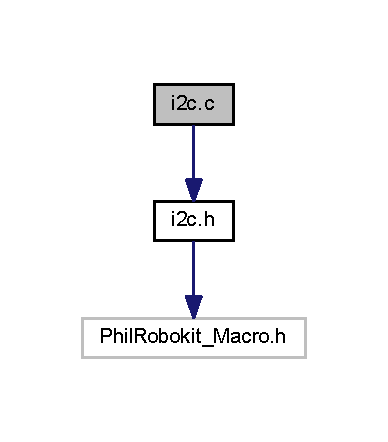
\includegraphics[width=186pt]{i2c_8c__incl}
\end{center}
\end{figure}
\subsection*{Functions}
\begin{DoxyCompactItemize}
\item 
void {\bf i2c\-Send\-Ack} (unsigned char uc\-S\-D\-A\-Pin, unsigned char uc\-S\-C\-L\-Pin, char bl\-Acknowledge)
\item 
void {\bf i2c\-Start} (unsigned char uc\-S\-D\-A\-Pin, unsigned char uc\-S\-C\-L\-Pin)
\item 
void {\bf i2c\-Stop} (unsigned char uc\-S\-D\-A\-Pin, unsigned char uc\-S\-C\-L\-Pin)
\item 
void {\bf setup\-I2\-C} (unsigned char uc\-S\-D\-A\-Pin, unsigned char uc\-S\-C\-L\-Pin)
\item 
void {\bf i2c\-Write} (unsigned char uc\-S\-D\-A\-Pin, unsigned char uc\-S\-C\-L\-Pin, unsigned char i2c\-Data)
\item 
unsigned char {\bf i2c\-Read} (unsigned char uc\-S\-D\-A\-Pin, unsigned char uc\-S\-C\-L\-Pin, char bl\-Acknowledge)
\end{DoxyCompactItemize}


\subsection{Function Documentation}
\index{i2c.\-c@{i2c.\-c}!i2c\-Read@{i2c\-Read}}
\index{i2c\-Read@{i2c\-Read}!i2c.c@{i2c.\-c}}
\subsubsection[{i2c\-Read}]{\setlength{\rightskip}{0pt plus 5cm}unsigned char i2c\-Read (
\begin{DoxyParamCaption}
\item[{unsigned char}]{uc\-S\-D\-A\-Pin, }
\item[{unsigned char}]{uc\-S\-C\-L\-Pin, }
\item[{char}]{bl\-Acknowledge}
\end{DoxyParamCaption}
)}\label{i2c_8c_aa04b90350a39d824dfc2af7cba74989d}


Definition at line 135 of file i2c.\-c.



Here is the call graph for this function\-:\nopagebreak
\begin{figure}[H]
\begin{center}
\leavevmode
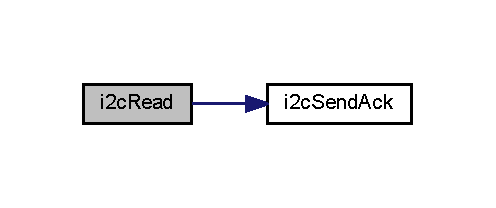
\includegraphics[width=238pt]{i2c_8c_aa04b90350a39d824dfc2af7cba74989d_cgraph}
\end{center}
\end{figure}


\index{i2c.\-c@{i2c.\-c}!i2c\-Send\-Ack@{i2c\-Send\-Ack}}
\index{i2c\-Send\-Ack@{i2c\-Send\-Ack}!i2c.c@{i2c.\-c}}
\subsubsection[{i2c\-Send\-Ack}]{\setlength{\rightskip}{0pt plus 5cm}void i2c\-Send\-Ack (
\begin{DoxyParamCaption}
\item[{unsigned char}]{uc\-S\-D\-A\-Pin, }
\item[{unsigned char}]{uc\-S\-C\-L\-Pin, }
\item[{char}]{bl\-Acknowledge}
\end{DoxyParamCaption}
)}\label{i2c_8c_ae9959378331903a98709ea582474c711}


Definition at line 37 of file i2c.\-c.

\index{i2c.\-c@{i2c.\-c}!i2c\-Start@{i2c\-Start}}
\index{i2c\-Start@{i2c\-Start}!i2c.c@{i2c.\-c}}
\subsubsection[{i2c\-Start}]{\setlength{\rightskip}{0pt plus 5cm}void i2c\-Start (
\begin{DoxyParamCaption}
\item[{unsigned char}]{uc\-S\-D\-A\-Pin, }
\item[{unsigned char}]{uc\-S\-C\-L\-Pin}
\end{DoxyParamCaption}
)}\label{i2c_8c_ab0ea860cc24c7c756b22820ac1c6c31d}


Definition at line 61 of file i2c.\-c.

\index{i2c.\-c@{i2c.\-c}!i2c\-Stop@{i2c\-Stop}}
\index{i2c\-Stop@{i2c\-Stop}!i2c.c@{i2c.\-c}}
\subsubsection[{i2c\-Stop}]{\setlength{\rightskip}{0pt plus 5cm}void i2c\-Stop (
\begin{DoxyParamCaption}
\item[{unsigned char}]{uc\-S\-D\-A\-Pin, }
\item[{unsigned char}]{uc\-S\-C\-L\-Pin}
\end{DoxyParamCaption}
)}\label{i2c_8c_a6a52e1291fa81bd690a7b8a420f13627}


Definition at line 73 of file i2c.\-c.

\index{i2c.\-c@{i2c.\-c}!i2c\-Write@{i2c\-Write}}
\index{i2c\-Write@{i2c\-Write}!i2c.c@{i2c.\-c}}
\subsubsection[{i2c\-Write}]{\setlength{\rightskip}{0pt plus 5cm}void i2c\-Write (
\begin{DoxyParamCaption}
\item[{unsigned char}]{uc\-S\-D\-A\-Pin, }
\item[{unsigned char}]{uc\-S\-C\-L\-Pin, }
\item[{unsigned char}]{i2c\-Data}
\end{DoxyParamCaption}
)}\label{i2c_8c_a7a80c7a4ac641b86203b814073859d90}


Definition at line 92 of file i2c.\-c.

\index{i2c.\-c@{i2c.\-c}!setup\-I2\-C@{setup\-I2\-C}}
\index{setup\-I2\-C@{setup\-I2\-C}!i2c.c@{i2c.\-c}}
\subsubsection[{setup\-I2\-C}]{\setlength{\rightskip}{0pt plus 5cm}void setup\-I2\-C (
\begin{DoxyParamCaption}
\item[{unsigned char}]{uc\-S\-D\-A\-Pin, }
\item[{unsigned char}]{uc\-S\-C\-L\-Pin}
\end{DoxyParamCaption}
)}\label{i2c_8c_a636c18124afd92a2540bb42538e2597d}


Definition at line 83 of file i2c.\-c.


\section{i2c.\-h File Reference}
\label{i2c_8h}\index{i2c.\-h@{i2c.\-h}}
{\ttfamily \#include \char`\"{}Phil\-Robokit\-\_\-\-Macro.\-h\char`\"{}}\\*
Include dependency graph for i2c.\-h\-:\nopagebreak
\begin{figure}[H]
\begin{center}
\leavevmode
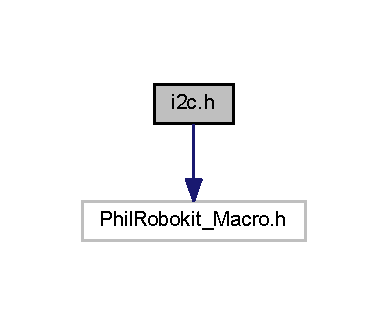
\includegraphics[width=186pt]{i2c_8h__incl}
\end{center}
\end{figure}
This graph shows which files directly or indirectly include this file\-:\nopagebreak
\begin{figure}[H]
\begin{center}
\leavevmode
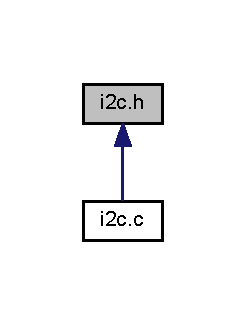
\includegraphics[width=118pt]{i2c_8h__dep__incl}
\end{center}
\end{figure}
\subsection*{Enumerations}
\begin{DoxyCompactItemize}
\item 
enum \{ {\bf I2\-C\-\_\-\-N\-O\-\_\-\-E\-R\-R\-O\-R}, 
{\bf I2\-C\-\_\-\-E\-R\-R\-O\-R\-\_\-\-N\-O\-\_\-\-A\-C\-K}
 \}
\end{DoxyCompactItemize}
\subsection*{Functions}
\begin{DoxyCompactItemize}
\item 
void {\bf i2c\-Send\-Ack} (unsigned char uc\-S\-D\-A\-Pin, unsigned char uc\-S\-C\-L\-Pin, char bl\-Acknowledge)
\item 
void {\bf i2c\-Start} (unsigned char uc\-S\-D\-A\-Pin, unsigned char uc\-S\-C\-L\-Pin)
\item 
void {\bf i2c\-Stop} (unsigned char uc\-S\-D\-A\-Pin, unsigned char uc\-S\-C\-L\-Pin)
\item 
void {\bf setup\-I2\-C} (unsigned char uc\-S\-D\-A\-Pin, unsigned char uc\-S\-C\-L\-Pin)
\item 
void {\bf i2c\-Write} (unsigned char uc\-S\-D\-A\-Pin, unsigned char uc\-S\-C\-L\-Pin, unsigned char i2c\-Data)
\item 
unsigned char {\bf i2c\-Read} (unsigned char uc\-S\-D\-A\-Pin, unsigned char uc\-S\-C\-L\-Pin, char bl\-Acknowledge)
\end{DoxyCompactItemize}


\subsection{Enumeration Type Documentation}
\subsubsection[{anonymous enum}]{\setlength{\rightskip}{0pt plus 5cm}anonymous enum}\label{i2c_8h_adf764cbdea00d65edcd07bb9953ad2b7}
\begin{Desc}
\item[Enumerator\-: ]\par
\begin{description}
\index{I2\-C\-\_\-\-N\-O\-\_\-\-E\-R\-R\-O\-R@{I2\-C\-\_\-\-N\-O\-\_\-\-E\-R\-R\-O\-R}!i2c.\-h@{i2c.\-h}}\index{i2c.\-h@{i2c.\-h}!I2\-C\-\_\-\-N\-O\-\_\-\-E\-R\-R\-O\-R@{I2\-C\-\_\-\-N\-O\-\_\-\-E\-R\-R\-O\-R}}\item[{\em 
I2\-C\-\_\-\-N\-O\-\_\-\-E\-R\-R\-O\-R\label{i2c_8h_adf764cbdea00d65edcd07bb9953ad2b7a0e9accb1d5f274c7dbd9c96a8178fc89}
}]\index{I2\-C\-\_\-\-E\-R\-R\-O\-R\-\_\-\-N\-O\-\_\-\-A\-C\-K@{I2\-C\-\_\-\-E\-R\-R\-O\-R\-\_\-\-N\-O\-\_\-\-A\-C\-K}!i2c.\-h@{i2c.\-h}}\index{i2c.\-h@{i2c.\-h}!I2\-C\-\_\-\-E\-R\-R\-O\-R\-\_\-\-N\-O\-\_\-\-A\-C\-K@{I2\-C\-\_\-\-E\-R\-R\-O\-R\-\_\-\-N\-O\-\_\-\-A\-C\-K}}\item[{\em 
I2\-C\-\_\-\-E\-R\-R\-O\-R\-\_\-\-N\-O\-\_\-\-A\-C\-K\label{i2c_8h_adf764cbdea00d65edcd07bb9953ad2b7a0275e17d7e045274d282fc85513f9243}
}]\end{description}
\end{Desc}



Definition at line 48 of file i2c.\-h.



\subsection{Function Documentation}
\index{i2c.\-h@{i2c.\-h}!i2c\-Read@{i2c\-Read}}
\index{i2c\-Read@{i2c\-Read}!i2c.h@{i2c.\-h}}
\subsubsection[{i2c\-Read}]{\setlength{\rightskip}{0pt plus 5cm}unsigned char i2c\-Read (
\begin{DoxyParamCaption}
\item[{unsigned char}]{uc\-S\-D\-A\-Pin, }
\item[{unsigned char}]{uc\-S\-C\-L\-Pin, }
\item[{char}]{bl\-Acknowledge}
\end{DoxyParamCaption}
)}\label{i2c_8h_aa04b90350a39d824dfc2af7cba74989d}


Definition at line 135 of file i2c.\-c.



Here is the call graph for this function\-:\nopagebreak
\begin{figure}[H]
\begin{center}
\leavevmode
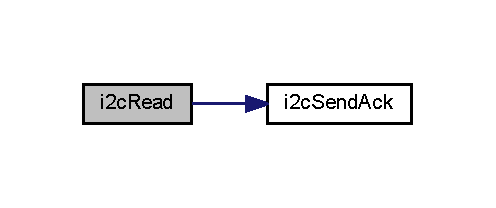
\includegraphics[width=238pt]{i2c_8h_aa04b90350a39d824dfc2af7cba74989d_cgraph}
\end{center}
\end{figure}


\index{i2c.\-h@{i2c.\-h}!i2c\-Send\-Ack@{i2c\-Send\-Ack}}
\index{i2c\-Send\-Ack@{i2c\-Send\-Ack}!i2c.h@{i2c.\-h}}
\subsubsection[{i2c\-Send\-Ack}]{\setlength{\rightskip}{0pt plus 5cm}void i2c\-Send\-Ack (
\begin{DoxyParamCaption}
\item[{unsigned char}]{uc\-S\-D\-A\-Pin, }
\item[{unsigned char}]{uc\-S\-C\-L\-Pin, }
\item[{char}]{bl\-Acknowledge}
\end{DoxyParamCaption}
)}\label{i2c_8h_ae9959378331903a98709ea582474c711}


Definition at line 37 of file i2c.\-c.

\index{i2c.\-h@{i2c.\-h}!i2c\-Start@{i2c\-Start}}
\index{i2c\-Start@{i2c\-Start}!i2c.h@{i2c.\-h}}
\subsubsection[{i2c\-Start}]{\setlength{\rightskip}{0pt plus 5cm}void i2c\-Start (
\begin{DoxyParamCaption}
\item[{unsigned char}]{uc\-S\-D\-A\-Pin, }
\item[{unsigned char}]{uc\-S\-C\-L\-Pin}
\end{DoxyParamCaption}
)}\label{i2c_8h_ab0ea860cc24c7c756b22820ac1c6c31d}


Definition at line 61 of file i2c.\-c.

\index{i2c.\-h@{i2c.\-h}!i2c\-Stop@{i2c\-Stop}}
\index{i2c\-Stop@{i2c\-Stop}!i2c.h@{i2c.\-h}}
\subsubsection[{i2c\-Stop}]{\setlength{\rightskip}{0pt plus 5cm}void i2c\-Stop (
\begin{DoxyParamCaption}
\item[{unsigned char}]{uc\-S\-D\-A\-Pin, }
\item[{unsigned char}]{uc\-S\-C\-L\-Pin}
\end{DoxyParamCaption}
)}\label{i2c_8h_a6a52e1291fa81bd690a7b8a420f13627}


Definition at line 73 of file i2c.\-c.

\index{i2c.\-h@{i2c.\-h}!i2c\-Write@{i2c\-Write}}
\index{i2c\-Write@{i2c\-Write}!i2c.h@{i2c.\-h}}
\subsubsection[{i2c\-Write}]{\setlength{\rightskip}{0pt plus 5cm}void i2c\-Write (
\begin{DoxyParamCaption}
\item[{unsigned char}]{uc\-S\-D\-A\-Pin, }
\item[{unsigned char}]{uc\-S\-C\-L\-Pin, }
\item[{unsigned char}]{i2c\-Data}
\end{DoxyParamCaption}
)}\label{i2c_8h_a7a80c7a4ac641b86203b814073859d90}


Definition at line 92 of file i2c.\-c.

\index{i2c.\-h@{i2c.\-h}!setup\-I2\-C@{setup\-I2\-C}}
\index{setup\-I2\-C@{setup\-I2\-C}!i2c.h@{i2c.\-h}}
\subsubsection[{setup\-I2\-C}]{\setlength{\rightskip}{0pt plus 5cm}void setup\-I2\-C (
\begin{DoxyParamCaption}
\item[{unsigned char}]{uc\-S\-D\-A\-Pin, }
\item[{unsigned char}]{uc\-S\-C\-L\-Pin}
\end{DoxyParamCaption}
)}\label{i2c_8h_a636c18124afd92a2540bb42538e2597d}


Definition at line 83 of file i2c.\-c.


\section{Multiple\-Servos.\-phr File Reference}
\label{_multiple_servos_8phr}\index{Multiple\-Servos.\-phr@{Multiple\-Servos.\-phr}}
{\ttfamily \#include $<$servo.\-h$>$}\\*
Include dependency graph for Multiple\-Servos.\-phr\-:\nopagebreak
\begin{figure}[H]
\begin{center}
\leavevmode
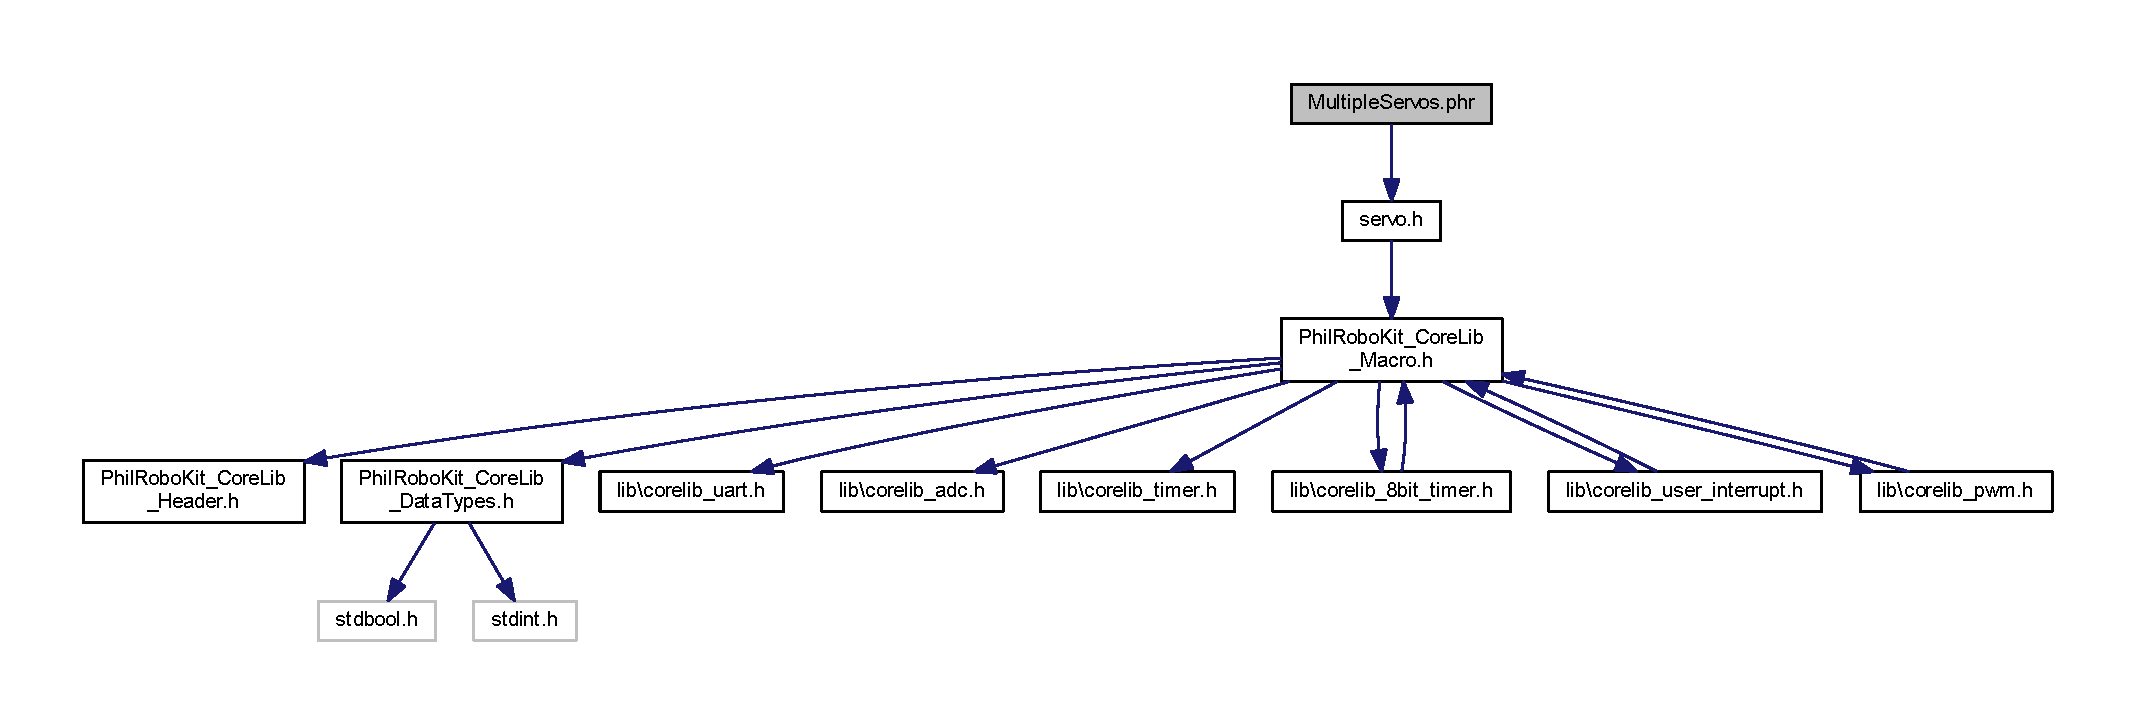
\includegraphics[width=350pt]{_multiple_servos_8phr__incl}
\end{center}
\end{figure}
\subsection*{Functions}
\begin{DoxyCompactItemize}
\item 
void {\bf init} ()
\item 
void {\bf program} ()
\end{DoxyCompactItemize}


\subsection{Function Documentation}
\index{Multiple\-Servos.\-phr@{Multiple\-Servos.\-phr}!init@{init}}
\index{init@{init}!MultipleServos.phr@{Multiple\-Servos.\-phr}}
\subsubsection[{init}]{\setlength{\rightskip}{0pt plus 5cm}void init (
\begin{DoxyParamCaption}
\item[{void}]{}
\end{DoxyParamCaption}
)}\label{_multiple_servos_8phr_a02fd73d861ef2e4aabb38c0c9ff82947}


Definition at line 3 of file Multiple\-Servos.\-phr.



Here is the call graph for this function\-:\nopagebreak
\begin{figure}[H]
\begin{center}
\leavevmode
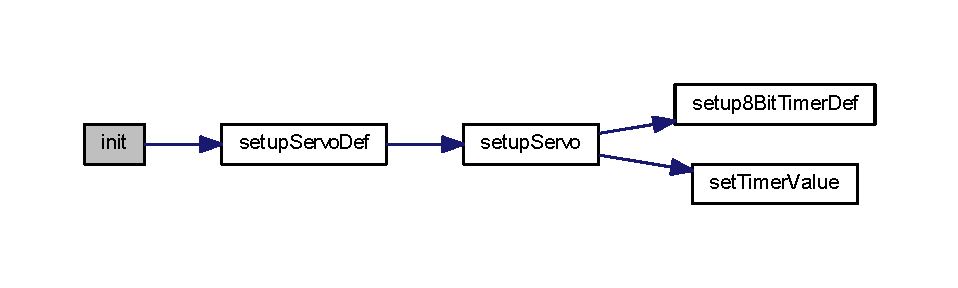
\includegraphics[width=350pt]{_multiple_servos_8phr_a02fd73d861ef2e4aabb38c0c9ff82947_cgraph}
\end{center}
\end{figure}


\index{Multiple\-Servos.\-phr@{Multiple\-Servos.\-phr}!program@{program}}
\index{program@{program}!MultipleServos.phr@{Multiple\-Servos.\-phr}}
\subsubsection[{program}]{\setlength{\rightskip}{0pt plus 5cm}void program (
\begin{DoxyParamCaption}
\item[{void}]{}
\end{DoxyParamCaption}
)}\label{_multiple_servos_8phr_aaed33fe77209e582d96078370b5f8da4}


Definition at line 15 of file Multiple\-Servos.\-phr.



Here is the call graph for this function\-:\nopagebreak
\begin{figure}[H]
\begin{center}
\leavevmode
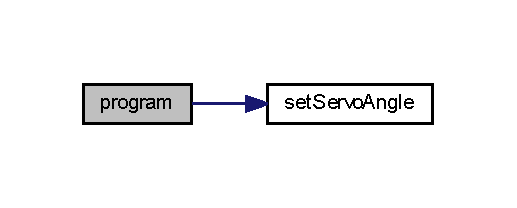
\includegraphics[width=248pt]{_multiple_servos_8phr_aaed33fe77209e582d96078370b5f8da4_cgraph}
\end{center}
\end{figure}



\section{Phil\-Robo\-Kit\-\_\-\-Core\-Lib\-\_\-\-Data\-Types.\-h File Reference}
\label{_phil_robo_kit___core_lib___data_types_8h}\index{Phil\-Robo\-Kit\-\_\-\-Core\-Lib\-\_\-\-Data\-Types.\-h@{Phil\-Robo\-Kit\-\_\-\-Core\-Lib\-\_\-\-Data\-Types.\-h}}
{\ttfamily \#include $<$stdbool.\-h$>$}\\*
{\ttfamily \#include $<$stdint.\-h$>$}\\*
Include dependency graph for Phil\-Robo\-Kit\-\_\-\-Core\-Lib\-\_\-\-Data\-Types.\-h\-:\nopagebreak
\begin{figure}[H]
\begin{center}
\leavevmode
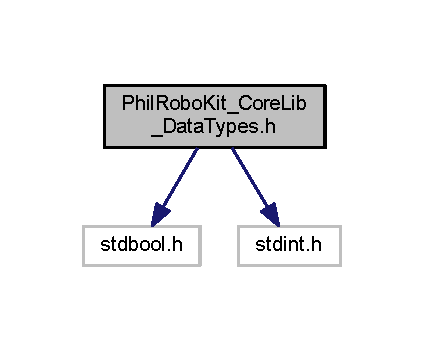
\includegraphics[width=203pt]{_phil_robo_kit___core_lib___data_types_8h__incl}
\end{center}
\end{figure}
This graph shows which files directly or indirectly include this file\-:\nopagebreak
\begin{figure}[H]
\begin{center}
\leavevmode
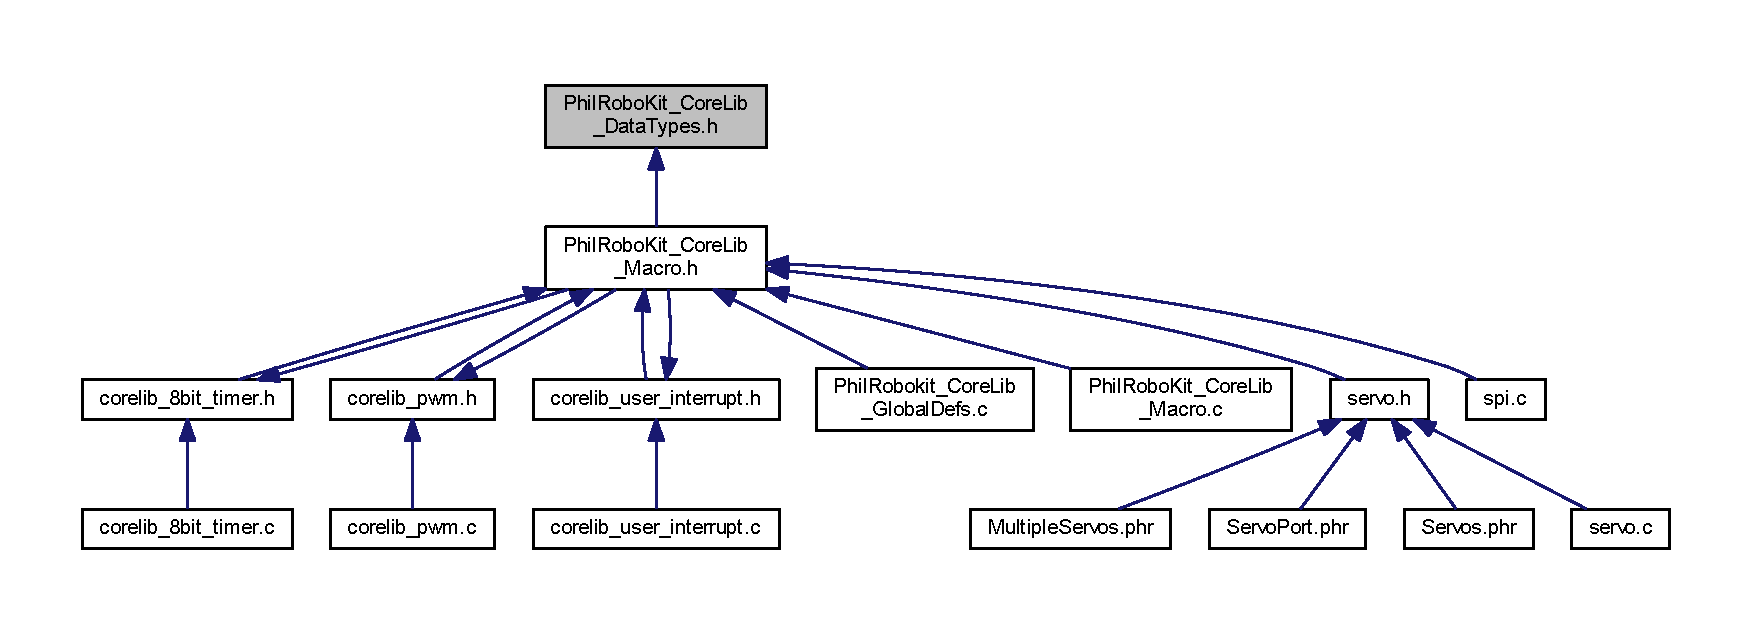
\includegraphics[width=350pt]{_phil_robo_kit___core_lib___data_types_8h__dep__incl}
\end{center}
\end{figure}

\section{Phil\-Robokit\-\_\-\-Core\-Lib\-\_\-\-Global\-Defs.\-c File Reference}
\label{_phil_robokit___core_lib___global_defs_8c}\index{Phil\-Robokit\-\_\-\-Core\-Lib\-\_\-\-Global\-Defs.\-c@{Phil\-Robokit\-\_\-\-Core\-Lib\-\_\-\-Global\-Defs.\-c}}
{\ttfamily \#include $<$Phil\-Robo\-Kit\-\_\-\-Core\-Lib\-\_\-\-Macro.\-h$>$}\\*
Include dependency graph for Phil\-Robokit\-\_\-\-Core\-Lib\-\_\-\-Global\-Defs.\-c\-:\nopagebreak
\begin{figure}[H]
\begin{center}
\leavevmode
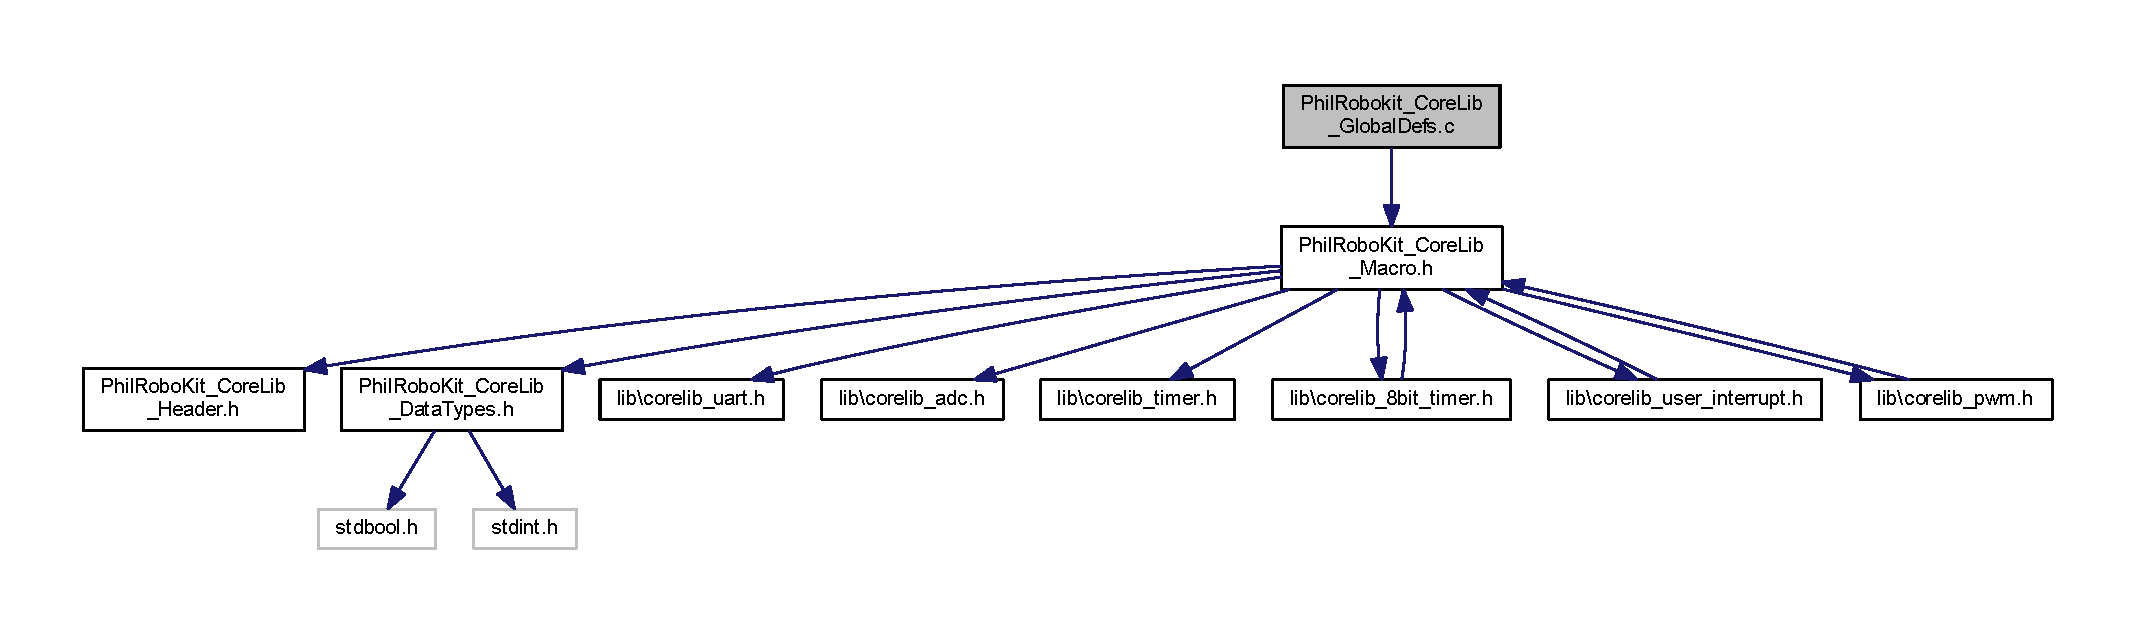
\includegraphics[width=350pt]{_phil_robokit___core_lib___global_defs_8c__incl}
\end{center}
\end{figure}

\section{Phil\-Robo\-Kit\-\_\-\-Core\-Lib\-\_\-\-Header.\-h File Reference}
\label{_phil_robo_kit___core_lib___header_8h}\index{Phil\-Robo\-Kit\-\_\-\-Core\-Lib\-\_\-\-Header.\-h@{Phil\-Robo\-Kit\-\_\-\-Core\-Lib\-\_\-\-Header.\-h}}
This graph shows which files directly or indirectly include this file\-:\nopagebreak
\begin{figure}[H]
\begin{center}
\leavevmode
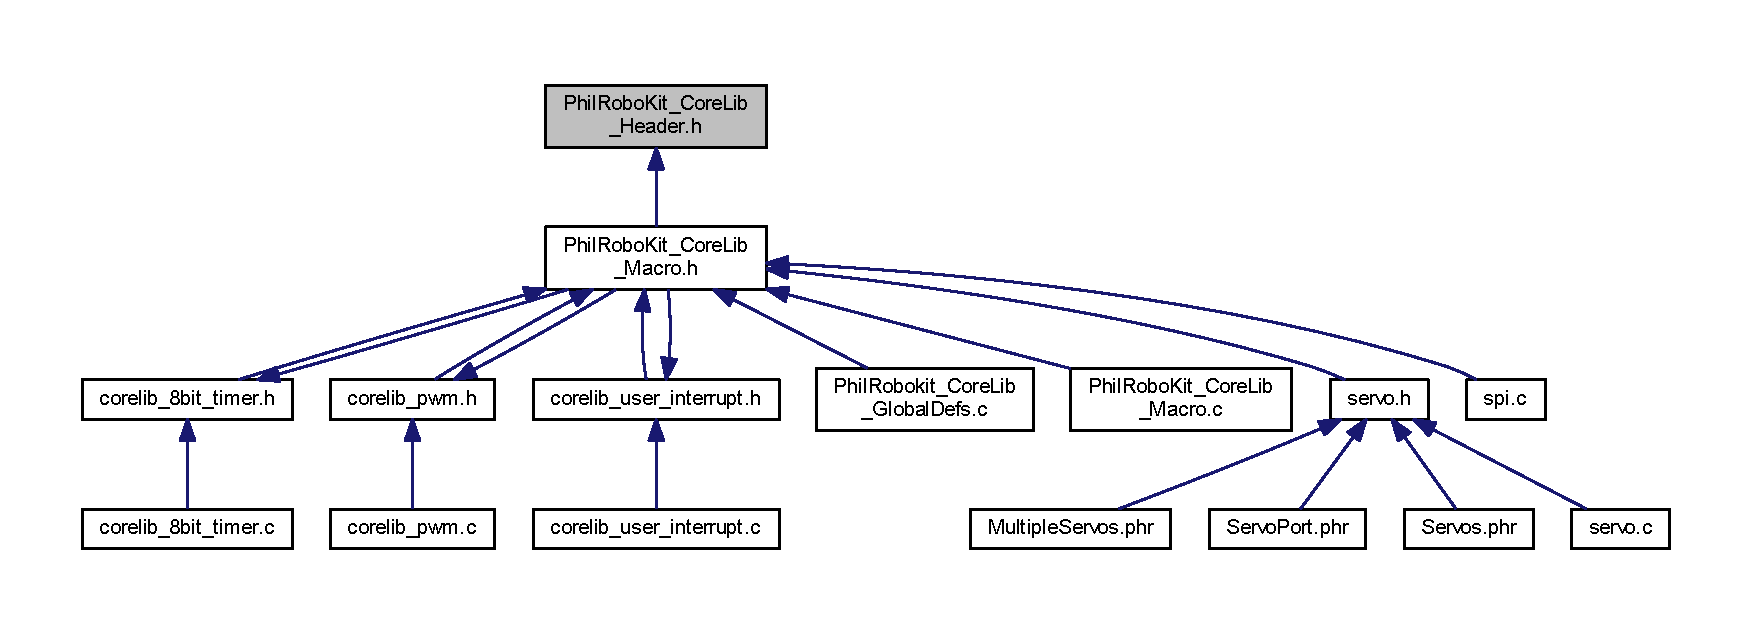
\includegraphics[width=350pt]{_phil_robo_kit___core_lib___header_8h__dep__incl}
\end{center}
\end{figure}
\subsection*{Macros}
\begin{DoxyCompactItemize}
\item 
\#define {\bf P\-I\-N0}~{\bf D0}
\item 
\#define {\bf P\-I\-N1}~{\bf D1}
\item 
\#define {\bf P\-I\-N2}~{\bf D2}
\item 
\#define {\bf P\-I\-N3}~{\bf D3}
\item 
\#define {\bf P\-I\-N4}~{\bf D4}
\item 
\#define {\bf P\-I\-N5}~{\bf D5}
\item 
\#define {\bf P\-I\-N6}~{\bf D6}
\item 
\#define {\bf P\-I\-N7}~{\bf D7}
\item 
\#define {\bf P\-I\-N8}~{\bf D8}
\item 
\#define {\bf P\-I\-N9}~{\bf D9}
\item 
\#define {\bf P\-I\-N10}~{\bf D10}
\item 
\#define {\bf P\-I\-N11}~{\bf D11}
\item 
\#define {\bf P\-I\-N12}~{\bf D12}
\item 
\#define {\bf P\-I\-N13}~{\bf D13}
\item 
\#define {\bf P\-I\-N14}~{\bf D14}
\item 
\#define {\bf P\-I\-N15}~{\bf D15}
\item 
\#define {\bf P\-I\-N16}~{\bf D16}
\item 
\#define {\bf P\-I\-N17}~{\bf D17}
\item 
\#define {\bf P\-I\-N18}~{\bf D18}
\item 
\#define {\bf P\-I\-N19}~{\bf D19}
\item 
\#define {\bf P\-I\-N20}~{\bf D20}
\item 
\#define {\bf A\-N0}~{\bf A0}
\item 
\#define {\bf A\-N1}~{\bf A1}
\item 
\#define {\bf A\-N2}~{\bf A2}
\item 
\#define {\bf A\-N3}~{\bf A3}
\item 
\#define {\bf A\-N4}~{\bf A4}
\item 
\#define {\bf A\-N5}~{\bf A5}
\item 
\#define {\bf A\-N6}~{\bf A6}
\item 
\#define {\bf L\-E\-D1}~{\bf L1}
\item 
\#define {\bf L\-E\-D2}~{\bf L2}
\item 
\#define {\bf L\-E\-D3}~{\bf L3}
\item 
\#define {\bf L\-E\-D4}~{\bf L4}
\item 
\#define {\bf S\-W1}~{\bf S1}
\item 
\#define {\bf S\-W2}~{\bf S2}
\item 
\#define {\bf S\-E\-R\-V\-O}~{\bf S\-R\-V}
\item 
\#define {\bf B\-U\-Z\-Z\-E\-R}~{\bf B\-U\-Z\-Z}
\item 
\#define {\bf C\-O\-N\-S\-T\-\_\-\-D\-E\-F\-A\-U\-L\-T\-\_\-\-C\-O\-N\-F\-I\-G\-\_\-\-P\-O\-R\-T\-A}~0b11111
\item 
\#define {\bf C\-O\-N\-S\-T\-\_\-\-D\-E\-F\-A\-U\-L\-T\-\_\-\-C\-O\-N\-F\-I\-G\-\_\-\-P\-O\-R\-T\-B}~0b00000000
\item 
\#define {\bf C\-O\-N\-S\-T\-\_\-\-D\-E\-F\-A\-U\-L\-T\-\_\-\-C\-O\-N\-F\-I\-G\-\_\-\-P\-O\-R\-T\-C}~0b10000000
\item 
\#define {\bf C\-O\-N\-S\-T\-\_\-\-D\-E\-F\-A\-U\-L\-T\-\_\-\-C\-O\-N\-F\-I\-G\-\_\-\-P\-O\-R\-T\-D}~0b00001100
\item 
\#define {\bf C\-O\-N\-S\-T\-\_\-\-D\-E\-F\-A\-U\-L\-T\-\_\-\-C\-O\-N\-F\-I\-G\-\_\-\-P\-O\-R\-T\-E}~0b111
\end{DoxyCompactItemize}
\subsection*{Enumerations}
\begin{DoxyCompactItemize}
\item 
enum {\bf Phil\-Robokit\-Pins} \{ \\*
{\bf D0} = 0, 
{\bf D1}, 
{\bf D2}, 
{\bf D3}, 
\\*
{\bf D4}, 
{\bf D5}, 
{\bf D6}, 
{\bf D7}, 
\\*
{\bf D8}, 
{\bf D9}, 
{\bf D10}, 
{\bf D11}, 
\\*
{\bf D12}, 
{\bf D13}, 
{\bf D14}, 
{\bf D15}, 
\\*
{\bf D16}, 
{\bf D17}, 
{\bf D18}, 
{\bf D19}, 
\\*
{\bf D20}, 
{\bf S\-R\-V}, 
{\bf B\-U\-Z\-Z}, 
{\bf S2}, 
\\*
{\bf S1}, 
{\bf L4}, 
{\bf L3}, 
{\bf L2}, 
\\*
{\bf L1}, 
{\bf A0} = 0, 
{\bf A1}, 
{\bf A2}, 
\\*
{\bf A3}, 
{\bf A4}, 
{\bf A5}, 
{\bf A6}, 
\\*
{\bf A7}
 \}
\end{DoxyCompactItemize}


\subsection{Macro Definition Documentation}
\index{Phil\-Robo\-Kit\-\_\-\-Core\-Lib\-\_\-\-Header.\-h@{Phil\-Robo\-Kit\-\_\-\-Core\-Lib\-\_\-\-Header.\-h}!A\-N0@{A\-N0}}
\index{A\-N0@{A\-N0}!PhilRoboKit_CoreLib_Header.h@{Phil\-Robo\-Kit\-\_\-\-Core\-Lib\-\_\-\-Header.\-h}}
\subsubsection[{A\-N0}]{\setlength{\rightskip}{0pt plus 5cm}\#define A\-N0~{\bf A0}}\label{_phil_robo_kit___core_lib___header_8h_a099995994c74b5fff8f7de4ff3eac550}


Definition at line 130 of file Phil\-Robo\-Kit\-\_\-\-Core\-Lib\-\_\-\-Header.\-h.

\index{Phil\-Robo\-Kit\-\_\-\-Core\-Lib\-\_\-\-Header.\-h@{Phil\-Robo\-Kit\-\_\-\-Core\-Lib\-\_\-\-Header.\-h}!A\-N1@{A\-N1}}
\index{A\-N1@{A\-N1}!PhilRoboKit_CoreLib_Header.h@{Phil\-Robo\-Kit\-\_\-\-Core\-Lib\-\_\-\-Header.\-h}}
\subsubsection[{A\-N1}]{\setlength{\rightskip}{0pt plus 5cm}\#define A\-N1~{\bf A1}}\label{_phil_robo_kit___core_lib___header_8h_a4903de2a52966c8dc2c20faf565d451d}


Definition at line 131 of file Phil\-Robo\-Kit\-\_\-\-Core\-Lib\-\_\-\-Header.\-h.

\index{Phil\-Robo\-Kit\-\_\-\-Core\-Lib\-\_\-\-Header.\-h@{Phil\-Robo\-Kit\-\_\-\-Core\-Lib\-\_\-\-Header.\-h}!A\-N2@{A\-N2}}
\index{A\-N2@{A\-N2}!PhilRoboKit_CoreLib_Header.h@{Phil\-Robo\-Kit\-\_\-\-Core\-Lib\-\_\-\-Header.\-h}}
\subsubsection[{A\-N2}]{\setlength{\rightskip}{0pt plus 5cm}\#define A\-N2~{\bf A2}}\label{_phil_robo_kit___core_lib___header_8h_a9b0754e893d69a1e69e856853f70da1f}


Definition at line 132 of file Phil\-Robo\-Kit\-\_\-\-Core\-Lib\-\_\-\-Header.\-h.

\index{Phil\-Robo\-Kit\-\_\-\-Core\-Lib\-\_\-\-Header.\-h@{Phil\-Robo\-Kit\-\_\-\-Core\-Lib\-\_\-\-Header.\-h}!A\-N3@{A\-N3}}
\index{A\-N3@{A\-N3}!PhilRoboKit_CoreLib_Header.h@{Phil\-Robo\-Kit\-\_\-\-Core\-Lib\-\_\-\-Header.\-h}}
\subsubsection[{A\-N3}]{\setlength{\rightskip}{0pt plus 5cm}\#define A\-N3~{\bf A3}}\label{_phil_robo_kit___core_lib___header_8h_a9f593faa38f1023698d74f03a457abe3}


Definition at line 133 of file Phil\-Robo\-Kit\-\_\-\-Core\-Lib\-\_\-\-Header.\-h.

\index{Phil\-Robo\-Kit\-\_\-\-Core\-Lib\-\_\-\-Header.\-h@{Phil\-Robo\-Kit\-\_\-\-Core\-Lib\-\_\-\-Header.\-h}!A\-N4@{A\-N4}}
\index{A\-N4@{A\-N4}!PhilRoboKit_CoreLib_Header.h@{Phil\-Robo\-Kit\-\_\-\-Core\-Lib\-\_\-\-Header.\-h}}
\subsubsection[{A\-N4}]{\setlength{\rightskip}{0pt plus 5cm}\#define A\-N4~{\bf A4}}\label{_phil_robo_kit___core_lib___header_8h_adc95f1e9cdc00268d7bca5885052171f}


Definition at line 134 of file Phil\-Robo\-Kit\-\_\-\-Core\-Lib\-\_\-\-Header.\-h.

\index{Phil\-Robo\-Kit\-\_\-\-Core\-Lib\-\_\-\-Header.\-h@{Phil\-Robo\-Kit\-\_\-\-Core\-Lib\-\_\-\-Header.\-h}!A\-N5@{A\-N5}}
\index{A\-N5@{A\-N5}!PhilRoboKit_CoreLib_Header.h@{Phil\-Robo\-Kit\-\_\-\-Core\-Lib\-\_\-\-Header.\-h}}
\subsubsection[{A\-N5}]{\setlength{\rightskip}{0pt plus 5cm}\#define A\-N5~{\bf A5}}\label{_phil_robo_kit___core_lib___header_8h_a99ed455a0d536be03f12eba18ccff71b}


Definition at line 135 of file Phil\-Robo\-Kit\-\_\-\-Core\-Lib\-\_\-\-Header.\-h.

\index{Phil\-Robo\-Kit\-\_\-\-Core\-Lib\-\_\-\-Header.\-h@{Phil\-Robo\-Kit\-\_\-\-Core\-Lib\-\_\-\-Header.\-h}!A\-N6@{A\-N6}}
\index{A\-N6@{A\-N6}!PhilRoboKit_CoreLib_Header.h@{Phil\-Robo\-Kit\-\_\-\-Core\-Lib\-\_\-\-Header.\-h}}
\subsubsection[{A\-N6}]{\setlength{\rightskip}{0pt plus 5cm}\#define A\-N6~{\bf A6}}\label{_phil_robo_kit___core_lib___header_8h_ad63d6861c3fa5e606de5c18ada3b4d10}


Definition at line 136 of file Phil\-Robo\-Kit\-\_\-\-Core\-Lib\-\_\-\-Header.\-h.

\index{Phil\-Robo\-Kit\-\_\-\-Core\-Lib\-\_\-\-Header.\-h@{Phil\-Robo\-Kit\-\_\-\-Core\-Lib\-\_\-\-Header.\-h}!B\-U\-Z\-Z\-E\-R@{B\-U\-Z\-Z\-E\-R}}
\index{B\-U\-Z\-Z\-E\-R@{B\-U\-Z\-Z\-E\-R}!PhilRoboKit_CoreLib_Header.h@{Phil\-Robo\-Kit\-\_\-\-Core\-Lib\-\_\-\-Header.\-h}}
\subsubsection[{B\-U\-Z\-Z\-E\-R}]{\setlength{\rightskip}{0pt plus 5cm}\#define B\-U\-Z\-Z\-E\-R~{\bf B\-U\-Z\-Z}}\label{_phil_robo_kit___core_lib___header_8h_a145103118f6d9d1129aa4509cf214a13}


Definition at line 148 of file Phil\-Robo\-Kit\-\_\-\-Core\-Lib\-\_\-\-Header.\-h.

\index{Phil\-Robo\-Kit\-\_\-\-Core\-Lib\-\_\-\-Header.\-h@{Phil\-Robo\-Kit\-\_\-\-Core\-Lib\-\_\-\-Header.\-h}!C\-O\-N\-S\-T\-\_\-\-D\-E\-F\-A\-U\-L\-T\-\_\-\-C\-O\-N\-F\-I\-G\-\_\-\-P\-O\-R\-T\-A@{C\-O\-N\-S\-T\-\_\-\-D\-E\-F\-A\-U\-L\-T\-\_\-\-C\-O\-N\-F\-I\-G\-\_\-\-P\-O\-R\-T\-A}}
\index{C\-O\-N\-S\-T\-\_\-\-D\-E\-F\-A\-U\-L\-T\-\_\-\-C\-O\-N\-F\-I\-G\-\_\-\-P\-O\-R\-T\-A@{C\-O\-N\-S\-T\-\_\-\-D\-E\-F\-A\-U\-L\-T\-\_\-\-C\-O\-N\-F\-I\-G\-\_\-\-P\-O\-R\-T\-A}!PhilRoboKit_CoreLib_Header.h@{Phil\-Robo\-Kit\-\_\-\-Core\-Lib\-\_\-\-Header.\-h}}
\subsubsection[{C\-O\-N\-S\-T\-\_\-\-D\-E\-F\-A\-U\-L\-T\-\_\-\-C\-O\-N\-F\-I\-G\-\_\-\-P\-O\-R\-T\-A}]{\setlength{\rightskip}{0pt plus 5cm}\#define C\-O\-N\-S\-T\-\_\-\-D\-E\-F\-A\-U\-L\-T\-\_\-\-C\-O\-N\-F\-I\-G\-\_\-\-P\-O\-R\-T\-A~0b11111}\label{_phil_robo_kit___core_lib___header_8h_ada906e4be4d194a311e6083c86488cc3}


Definition at line 153 of file Phil\-Robo\-Kit\-\_\-\-Core\-Lib\-\_\-\-Header.\-h.

\index{Phil\-Robo\-Kit\-\_\-\-Core\-Lib\-\_\-\-Header.\-h@{Phil\-Robo\-Kit\-\_\-\-Core\-Lib\-\_\-\-Header.\-h}!C\-O\-N\-S\-T\-\_\-\-D\-E\-F\-A\-U\-L\-T\-\_\-\-C\-O\-N\-F\-I\-G\-\_\-\-P\-O\-R\-T\-B@{C\-O\-N\-S\-T\-\_\-\-D\-E\-F\-A\-U\-L\-T\-\_\-\-C\-O\-N\-F\-I\-G\-\_\-\-P\-O\-R\-T\-B}}
\index{C\-O\-N\-S\-T\-\_\-\-D\-E\-F\-A\-U\-L\-T\-\_\-\-C\-O\-N\-F\-I\-G\-\_\-\-P\-O\-R\-T\-B@{C\-O\-N\-S\-T\-\_\-\-D\-E\-F\-A\-U\-L\-T\-\_\-\-C\-O\-N\-F\-I\-G\-\_\-\-P\-O\-R\-T\-B}!PhilRoboKit_CoreLib_Header.h@{Phil\-Robo\-Kit\-\_\-\-Core\-Lib\-\_\-\-Header.\-h}}
\subsubsection[{C\-O\-N\-S\-T\-\_\-\-D\-E\-F\-A\-U\-L\-T\-\_\-\-C\-O\-N\-F\-I\-G\-\_\-\-P\-O\-R\-T\-B}]{\setlength{\rightskip}{0pt plus 5cm}\#define C\-O\-N\-S\-T\-\_\-\-D\-E\-F\-A\-U\-L\-T\-\_\-\-C\-O\-N\-F\-I\-G\-\_\-\-P\-O\-R\-T\-B~0b00000000}\label{_phil_robo_kit___core_lib___header_8h_a5681f1f999e738eb0513216ffc1921f0}


Definition at line 154 of file Phil\-Robo\-Kit\-\_\-\-Core\-Lib\-\_\-\-Header.\-h.

\index{Phil\-Robo\-Kit\-\_\-\-Core\-Lib\-\_\-\-Header.\-h@{Phil\-Robo\-Kit\-\_\-\-Core\-Lib\-\_\-\-Header.\-h}!C\-O\-N\-S\-T\-\_\-\-D\-E\-F\-A\-U\-L\-T\-\_\-\-C\-O\-N\-F\-I\-G\-\_\-\-P\-O\-R\-T\-C@{C\-O\-N\-S\-T\-\_\-\-D\-E\-F\-A\-U\-L\-T\-\_\-\-C\-O\-N\-F\-I\-G\-\_\-\-P\-O\-R\-T\-C}}
\index{C\-O\-N\-S\-T\-\_\-\-D\-E\-F\-A\-U\-L\-T\-\_\-\-C\-O\-N\-F\-I\-G\-\_\-\-P\-O\-R\-T\-C@{C\-O\-N\-S\-T\-\_\-\-D\-E\-F\-A\-U\-L\-T\-\_\-\-C\-O\-N\-F\-I\-G\-\_\-\-P\-O\-R\-T\-C}!PhilRoboKit_CoreLib_Header.h@{Phil\-Robo\-Kit\-\_\-\-Core\-Lib\-\_\-\-Header.\-h}}
\subsubsection[{C\-O\-N\-S\-T\-\_\-\-D\-E\-F\-A\-U\-L\-T\-\_\-\-C\-O\-N\-F\-I\-G\-\_\-\-P\-O\-R\-T\-C}]{\setlength{\rightskip}{0pt plus 5cm}\#define C\-O\-N\-S\-T\-\_\-\-D\-E\-F\-A\-U\-L\-T\-\_\-\-C\-O\-N\-F\-I\-G\-\_\-\-P\-O\-R\-T\-C~0b10000000}\label{_phil_robo_kit___core_lib___header_8h_a0e12790a113a04f2dfb7cdfeffa71b2a}


Definition at line 155 of file Phil\-Robo\-Kit\-\_\-\-Core\-Lib\-\_\-\-Header.\-h.

\index{Phil\-Robo\-Kit\-\_\-\-Core\-Lib\-\_\-\-Header.\-h@{Phil\-Robo\-Kit\-\_\-\-Core\-Lib\-\_\-\-Header.\-h}!C\-O\-N\-S\-T\-\_\-\-D\-E\-F\-A\-U\-L\-T\-\_\-\-C\-O\-N\-F\-I\-G\-\_\-\-P\-O\-R\-T\-D@{C\-O\-N\-S\-T\-\_\-\-D\-E\-F\-A\-U\-L\-T\-\_\-\-C\-O\-N\-F\-I\-G\-\_\-\-P\-O\-R\-T\-D}}
\index{C\-O\-N\-S\-T\-\_\-\-D\-E\-F\-A\-U\-L\-T\-\_\-\-C\-O\-N\-F\-I\-G\-\_\-\-P\-O\-R\-T\-D@{C\-O\-N\-S\-T\-\_\-\-D\-E\-F\-A\-U\-L\-T\-\_\-\-C\-O\-N\-F\-I\-G\-\_\-\-P\-O\-R\-T\-D}!PhilRoboKit_CoreLib_Header.h@{Phil\-Robo\-Kit\-\_\-\-Core\-Lib\-\_\-\-Header.\-h}}
\subsubsection[{C\-O\-N\-S\-T\-\_\-\-D\-E\-F\-A\-U\-L\-T\-\_\-\-C\-O\-N\-F\-I\-G\-\_\-\-P\-O\-R\-T\-D}]{\setlength{\rightskip}{0pt plus 5cm}\#define C\-O\-N\-S\-T\-\_\-\-D\-E\-F\-A\-U\-L\-T\-\_\-\-C\-O\-N\-F\-I\-G\-\_\-\-P\-O\-R\-T\-D~0b00001100}\label{_phil_robo_kit___core_lib___header_8h_a3c70849d541b60deb4ab1e903f36cb51}


Definition at line 156 of file Phil\-Robo\-Kit\-\_\-\-Core\-Lib\-\_\-\-Header.\-h.

\index{Phil\-Robo\-Kit\-\_\-\-Core\-Lib\-\_\-\-Header.\-h@{Phil\-Robo\-Kit\-\_\-\-Core\-Lib\-\_\-\-Header.\-h}!C\-O\-N\-S\-T\-\_\-\-D\-E\-F\-A\-U\-L\-T\-\_\-\-C\-O\-N\-F\-I\-G\-\_\-\-P\-O\-R\-T\-E@{C\-O\-N\-S\-T\-\_\-\-D\-E\-F\-A\-U\-L\-T\-\_\-\-C\-O\-N\-F\-I\-G\-\_\-\-P\-O\-R\-T\-E}}
\index{C\-O\-N\-S\-T\-\_\-\-D\-E\-F\-A\-U\-L\-T\-\_\-\-C\-O\-N\-F\-I\-G\-\_\-\-P\-O\-R\-T\-E@{C\-O\-N\-S\-T\-\_\-\-D\-E\-F\-A\-U\-L\-T\-\_\-\-C\-O\-N\-F\-I\-G\-\_\-\-P\-O\-R\-T\-E}!PhilRoboKit_CoreLib_Header.h@{Phil\-Robo\-Kit\-\_\-\-Core\-Lib\-\_\-\-Header.\-h}}
\subsubsection[{C\-O\-N\-S\-T\-\_\-\-D\-E\-F\-A\-U\-L\-T\-\_\-\-C\-O\-N\-F\-I\-G\-\_\-\-P\-O\-R\-T\-E}]{\setlength{\rightskip}{0pt plus 5cm}\#define C\-O\-N\-S\-T\-\_\-\-D\-E\-F\-A\-U\-L\-T\-\_\-\-C\-O\-N\-F\-I\-G\-\_\-\-P\-O\-R\-T\-E~0b111}\label{_phil_robo_kit___core_lib___header_8h_ae215b7a6ba69b0f20459830a655ae931}


Definition at line 157 of file Phil\-Robo\-Kit\-\_\-\-Core\-Lib\-\_\-\-Header.\-h.

\index{Phil\-Robo\-Kit\-\_\-\-Core\-Lib\-\_\-\-Header.\-h@{Phil\-Robo\-Kit\-\_\-\-Core\-Lib\-\_\-\-Header.\-h}!L\-E\-D1@{L\-E\-D1}}
\index{L\-E\-D1@{L\-E\-D1}!PhilRoboKit_CoreLib_Header.h@{Phil\-Robo\-Kit\-\_\-\-Core\-Lib\-\_\-\-Header.\-h}}
\subsubsection[{L\-E\-D1}]{\setlength{\rightskip}{0pt plus 5cm}\#define L\-E\-D1~{\bf L1}}\label{_phil_robo_kit___core_lib___header_8h_a8aa85ae9867fabf70ec72cd3bf6fb6b9}


Definition at line 139 of file Phil\-Robo\-Kit\-\_\-\-Core\-Lib\-\_\-\-Header.\-h.

\index{Phil\-Robo\-Kit\-\_\-\-Core\-Lib\-\_\-\-Header.\-h@{Phil\-Robo\-Kit\-\_\-\-Core\-Lib\-\_\-\-Header.\-h}!L\-E\-D2@{L\-E\-D2}}
\index{L\-E\-D2@{L\-E\-D2}!PhilRoboKit_CoreLib_Header.h@{Phil\-Robo\-Kit\-\_\-\-Core\-Lib\-\_\-\-Header.\-h}}
\subsubsection[{L\-E\-D2}]{\setlength{\rightskip}{0pt plus 5cm}\#define L\-E\-D2~{\bf L2}}\label{_phil_robo_kit___core_lib___header_8h_ad09fe5bf321b9a2de26bd5e5b9af6424}


Definition at line 140 of file Phil\-Robo\-Kit\-\_\-\-Core\-Lib\-\_\-\-Header.\-h.

\index{Phil\-Robo\-Kit\-\_\-\-Core\-Lib\-\_\-\-Header.\-h@{Phil\-Robo\-Kit\-\_\-\-Core\-Lib\-\_\-\-Header.\-h}!L\-E\-D3@{L\-E\-D3}}
\index{L\-E\-D3@{L\-E\-D3}!PhilRoboKit_CoreLib_Header.h@{Phil\-Robo\-Kit\-\_\-\-Core\-Lib\-\_\-\-Header.\-h}}
\subsubsection[{L\-E\-D3}]{\setlength{\rightskip}{0pt plus 5cm}\#define L\-E\-D3~{\bf L3}}\label{_phil_robo_kit___core_lib___header_8h_a4b7ff8e253a7412f83deba3a447028a8}


Definition at line 141 of file Phil\-Robo\-Kit\-\_\-\-Core\-Lib\-\_\-\-Header.\-h.

\index{Phil\-Robo\-Kit\-\_\-\-Core\-Lib\-\_\-\-Header.\-h@{Phil\-Robo\-Kit\-\_\-\-Core\-Lib\-\_\-\-Header.\-h}!L\-E\-D4@{L\-E\-D4}}
\index{L\-E\-D4@{L\-E\-D4}!PhilRoboKit_CoreLib_Header.h@{Phil\-Robo\-Kit\-\_\-\-Core\-Lib\-\_\-\-Header.\-h}}
\subsubsection[{L\-E\-D4}]{\setlength{\rightskip}{0pt plus 5cm}\#define L\-E\-D4~{\bf L4}}\label{_phil_robo_kit___core_lib___header_8h_ae048837f20072bed467332b1bd1da9fa}


Definition at line 142 of file Phil\-Robo\-Kit\-\_\-\-Core\-Lib\-\_\-\-Header.\-h.

\index{Phil\-Robo\-Kit\-\_\-\-Core\-Lib\-\_\-\-Header.\-h@{Phil\-Robo\-Kit\-\_\-\-Core\-Lib\-\_\-\-Header.\-h}!P\-I\-N0@{P\-I\-N0}}
\index{P\-I\-N0@{P\-I\-N0}!PhilRoboKit_CoreLib_Header.h@{Phil\-Robo\-Kit\-\_\-\-Core\-Lib\-\_\-\-Header.\-h}}
\subsubsection[{P\-I\-N0}]{\setlength{\rightskip}{0pt plus 5cm}\#define P\-I\-N0~{\bf D0}}\label{_phil_robo_kit___core_lib___header_8h_a8909e4cc8d1f05aeb73943042144abdf}


Definition at line 105 of file Phil\-Robo\-Kit\-\_\-\-Core\-Lib\-\_\-\-Header.\-h.

\index{Phil\-Robo\-Kit\-\_\-\-Core\-Lib\-\_\-\-Header.\-h@{Phil\-Robo\-Kit\-\_\-\-Core\-Lib\-\_\-\-Header.\-h}!P\-I\-N1@{P\-I\-N1}}
\index{P\-I\-N1@{P\-I\-N1}!PhilRoboKit_CoreLib_Header.h@{Phil\-Robo\-Kit\-\_\-\-Core\-Lib\-\_\-\-Header.\-h}}
\subsubsection[{P\-I\-N1}]{\setlength{\rightskip}{0pt plus 5cm}\#define P\-I\-N1~{\bf D1}}\label{_phil_robo_kit___core_lib___header_8h_a522e24eb599eab6d1ec4b1ae5a3a12b2}


Definition at line 106 of file Phil\-Robo\-Kit\-\_\-\-Core\-Lib\-\_\-\-Header.\-h.

\index{Phil\-Robo\-Kit\-\_\-\-Core\-Lib\-\_\-\-Header.\-h@{Phil\-Robo\-Kit\-\_\-\-Core\-Lib\-\_\-\-Header.\-h}!P\-I\-N10@{P\-I\-N10}}
\index{P\-I\-N10@{P\-I\-N10}!PhilRoboKit_CoreLib_Header.h@{Phil\-Robo\-Kit\-\_\-\-Core\-Lib\-\_\-\-Header.\-h}}
\subsubsection[{P\-I\-N10}]{\setlength{\rightskip}{0pt plus 5cm}\#define P\-I\-N10~{\bf D10}}\label{_phil_robo_kit___core_lib___header_8h_acbaa6d4a20c4676abf31008f0bfcbe70}


Definition at line 116 of file Phil\-Robo\-Kit\-\_\-\-Core\-Lib\-\_\-\-Header.\-h.

\index{Phil\-Robo\-Kit\-\_\-\-Core\-Lib\-\_\-\-Header.\-h@{Phil\-Robo\-Kit\-\_\-\-Core\-Lib\-\_\-\-Header.\-h}!P\-I\-N11@{P\-I\-N11}}
\index{P\-I\-N11@{P\-I\-N11}!PhilRoboKit_CoreLib_Header.h@{Phil\-Robo\-Kit\-\_\-\-Core\-Lib\-\_\-\-Header.\-h}}
\subsubsection[{P\-I\-N11}]{\setlength{\rightskip}{0pt plus 5cm}\#define P\-I\-N11~{\bf D11}}\label{_phil_robo_kit___core_lib___header_8h_adcf2cdf444ef9ba3ec75f8adf6b3fa13}


Definition at line 117 of file Phil\-Robo\-Kit\-\_\-\-Core\-Lib\-\_\-\-Header.\-h.

\index{Phil\-Robo\-Kit\-\_\-\-Core\-Lib\-\_\-\-Header.\-h@{Phil\-Robo\-Kit\-\_\-\-Core\-Lib\-\_\-\-Header.\-h}!P\-I\-N12@{P\-I\-N12}}
\index{P\-I\-N12@{P\-I\-N12}!PhilRoboKit_CoreLib_Header.h@{Phil\-Robo\-Kit\-\_\-\-Core\-Lib\-\_\-\-Header.\-h}}
\subsubsection[{P\-I\-N12}]{\setlength{\rightskip}{0pt plus 5cm}\#define P\-I\-N12~{\bf D12}}\label{_phil_robo_kit___core_lib___header_8h_a0157ab3e88e2635fceafe002a02cec6e}


Definition at line 118 of file Phil\-Robo\-Kit\-\_\-\-Core\-Lib\-\_\-\-Header.\-h.

\index{Phil\-Robo\-Kit\-\_\-\-Core\-Lib\-\_\-\-Header.\-h@{Phil\-Robo\-Kit\-\_\-\-Core\-Lib\-\_\-\-Header.\-h}!P\-I\-N13@{P\-I\-N13}}
\index{P\-I\-N13@{P\-I\-N13}!PhilRoboKit_CoreLib_Header.h@{Phil\-Robo\-Kit\-\_\-\-Core\-Lib\-\_\-\-Header.\-h}}
\subsubsection[{P\-I\-N13}]{\setlength{\rightskip}{0pt plus 5cm}\#define P\-I\-N13~{\bf D13}}\label{_phil_robo_kit___core_lib___header_8h_a5a4d13c57f4d208901b04a7044774293}


Definition at line 119 of file Phil\-Robo\-Kit\-\_\-\-Core\-Lib\-\_\-\-Header.\-h.

\index{Phil\-Robo\-Kit\-\_\-\-Core\-Lib\-\_\-\-Header.\-h@{Phil\-Robo\-Kit\-\_\-\-Core\-Lib\-\_\-\-Header.\-h}!P\-I\-N14@{P\-I\-N14}}
\index{P\-I\-N14@{P\-I\-N14}!PhilRoboKit_CoreLib_Header.h@{Phil\-Robo\-Kit\-\_\-\-Core\-Lib\-\_\-\-Header.\-h}}
\subsubsection[{P\-I\-N14}]{\setlength{\rightskip}{0pt plus 5cm}\#define P\-I\-N14~{\bf D14}}\label{_phil_robo_kit___core_lib___header_8h_aa4645c06dfc42a41fc6a986de213ce10}


Definition at line 122 of file Phil\-Robo\-Kit\-\_\-\-Core\-Lib\-\_\-\-Header.\-h.

\index{Phil\-Robo\-Kit\-\_\-\-Core\-Lib\-\_\-\-Header.\-h@{Phil\-Robo\-Kit\-\_\-\-Core\-Lib\-\_\-\-Header.\-h}!P\-I\-N15@{P\-I\-N15}}
\index{P\-I\-N15@{P\-I\-N15}!PhilRoboKit_CoreLib_Header.h@{Phil\-Robo\-Kit\-\_\-\-Core\-Lib\-\_\-\-Header.\-h}}
\subsubsection[{P\-I\-N15}]{\setlength{\rightskip}{0pt plus 5cm}\#define P\-I\-N15~{\bf D15}}\label{_phil_robo_kit___core_lib___header_8h_aaaf21acf9f0278d91c9f253b417ab9ad}


Definition at line 123 of file Phil\-Robo\-Kit\-\_\-\-Core\-Lib\-\_\-\-Header.\-h.

\index{Phil\-Robo\-Kit\-\_\-\-Core\-Lib\-\_\-\-Header.\-h@{Phil\-Robo\-Kit\-\_\-\-Core\-Lib\-\_\-\-Header.\-h}!P\-I\-N16@{P\-I\-N16}}
\index{P\-I\-N16@{P\-I\-N16}!PhilRoboKit_CoreLib_Header.h@{Phil\-Robo\-Kit\-\_\-\-Core\-Lib\-\_\-\-Header.\-h}}
\subsubsection[{P\-I\-N16}]{\setlength{\rightskip}{0pt plus 5cm}\#define P\-I\-N16~{\bf D16}}\label{_phil_robo_kit___core_lib___header_8h_aa8a0f35acb2789eeeecec0b656a199b0}


Definition at line 124 of file Phil\-Robo\-Kit\-\_\-\-Core\-Lib\-\_\-\-Header.\-h.

\index{Phil\-Robo\-Kit\-\_\-\-Core\-Lib\-\_\-\-Header.\-h@{Phil\-Robo\-Kit\-\_\-\-Core\-Lib\-\_\-\-Header.\-h}!P\-I\-N17@{P\-I\-N17}}
\index{P\-I\-N17@{P\-I\-N17}!PhilRoboKit_CoreLib_Header.h@{Phil\-Robo\-Kit\-\_\-\-Core\-Lib\-\_\-\-Header.\-h}}
\subsubsection[{P\-I\-N17}]{\setlength{\rightskip}{0pt plus 5cm}\#define P\-I\-N17~{\bf D17}}\label{_phil_robo_kit___core_lib___header_8h_a93d4abbc247fea643613b5b34bc5c8e8}


Definition at line 125 of file Phil\-Robo\-Kit\-\_\-\-Core\-Lib\-\_\-\-Header.\-h.

\index{Phil\-Robo\-Kit\-\_\-\-Core\-Lib\-\_\-\-Header.\-h@{Phil\-Robo\-Kit\-\_\-\-Core\-Lib\-\_\-\-Header.\-h}!P\-I\-N18@{P\-I\-N18}}
\index{P\-I\-N18@{P\-I\-N18}!PhilRoboKit_CoreLib_Header.h@{Phil\-Robo\-Kit\-\_\-\-Core\-Lib\-\_\-\-Header.\-h}}
\subsubsection[{P\-I\-N18}]{\setlength{\rightskip}{0pt plus 5cm}\#define P\-I\-N18~{\bf D18}}\label{_phil_robo_kit___core_lib___header_8h_a42dbee90edd2f61e90f501fa3f667761}


Definition at line 126 of file Phil\-Robo\-Kit\-\_\-\-Core\-Lib\-\_\-\-Header.\-h.

\index{Phil\-Robo\-Kit\-\_\-\-Core\-Lib\-\_\-\-Header.\-h@{Phil\-Robo\-Kit\-\_\-\-Core\-Lib\-\_\-\-Header.\-h}!P\-I\-N19@{P\-I\-N19}}
\index{P\-I\-N19@{P\-I\-N19}!PhilRoboKit_CoreLib_Header.h@{Phil\-Robo\-Kit\-\_\-\-Core\-Lib\-\_\-\-Header.\-h}}
\subsubsection[{P\-I\-N19}]{\setlength{\rightskip}{0pt plus 5cm}\#define P\-I\-N19~{\bf D19}}\label{_phil_robo_kit___core_lib___header_8h_aff004b7e49bf7b38d964e00e93707a0a}


Definition at line 127 of file Phil\-Robo\-Kit\-\_\-\-Core\-Lib\-\_\-\-Header.\-h.

\index{Phil\-Robo\-Kit\-\_\-\-Core\-Lib\-\_\-\-Header.\-h@{Phil\-Robo\-Kit\-\_\-\-Core\-Lib\-\_\-\-Header.\-h}!P\-I\-N2@{P\-I\-N2}}
\index{P\-I\-N2@{P\-I\-N2}!PhilRoboKit_CoreLib_Header.h@{Phil\-Robo\-Kit\-\_\-\-Core\-Lib\-\_\-\-Header.\-h}}
\subsubsection[{P\-I\-N2}]{\setlength{\rightskip}{0pt plus 5cm}\#define P\-I\-N2~{\bf D2}}\label{_phil_robo_kit___core_lib___header_8h_a903210ad84aed4458cbc75b489f9bb7e}


Definition at line 107 of file Phil\-Robo\-Kit\-\_\-\-Core\-Lib\-\_\-\-Header.\-h.

\index{Phil\-Robo\-Kit\-\_\-\-Core\-Lib\-\_\-\-Header.\-h@{Phil\-Robo\-Kit\-\_\-\-Core\-Lib\-\_\-\-Header.\-h}!P\-I\-N20@{P\-I\-N20}}
\index{P\-I\-N20@{P\-I\-N20}!PhilRoboKit_CoreLib_Header.h@{Phil\-Robo\-Kit\-\_\-\-Core\-Lib\-\_\-\-Header.\-h}}
\subsubsection[{P\-I\-N20}]{\setlength{\rightskip}{0pt plus 5cm}\#define P\-I\-N20~{\bf D20}}\label{_phil_robo_kit___core_lib___header_8h_abe070c4481f21aea347ea871ddabf922}


Definition at line 128 of file Phil\-Robo\-Kit\-\_\-\-Core\-Lib\-\_\-\-Header.\-h.

\index{Phil\-Robo\-Kit\-\_\-\-Core\-Lib\-\_\-\-Header.\-h@{Phil\-Robo\-Kit\-\_\-\-Core\-Lib\-\_\-\-Header.\-h}!P\-I\-N3@{P\-I\-N3}}
\index{P\-I\-N3@{P\-I\-N3}!PhilRoboKit_CoreLib_Header.h@{Phil\-Robo\-Kit\-\_\-\-Core\-Lib\-\_\-\-Header.\-h}}
\subsubsection[{P\-I\-N3}]{\setlength{\rightskip}{0pt plus 5cm}\#define P\-I\-N3~{\bf D3}}\label{_phil_robo_kit___core_lib___header_8h_ac4b639acb4bf160a49ff3c0d8fa80fc4}


Definition at line 108 of file Phil\-Robo\-Kit\-\_\-\-Core\-Lib\-\_\-\-Header.\-h.

\index{Phil\-Robo\-Kit\-\_\-\-Core\-Lib\-\_\-\-Header.\-h@{Phil\-Robo\-Kit\-\_\-\-Core\-Lib\-\_\-\-Header.\-h}!P\-I\-N4@{P\-I\-N4}}
\index{P\-I\-N4@{P\-I\-N4}!PhilRoboKit_CoreLib_Header.h@{Phil\-Robo\-Kit\-\_\-\-Core\-Lib\-\_\-\-Header.\-h}}
\subsubsection[{P\-I\-N4}]{\setlength{\rightskip}{0pt plus 5cm}\#define P\-I\-N4~{\bf D4}}\label{_phil_robo_kit___core_lib___header_8h_aa3a35a41c5285c9c632aa626ac6761cb}


Definition at line 109 of file Phil\-Robo\-Kit\-\_\-\-Core\-Lib\-\_\-\-Header.\-h.

\index{Phil\-Robo\-Kit\-\_\-\-Core\-Lib\-\_\-\-Header.\-h@{Phil\-Robo\-Kit\-\_\-\-Core\-Lib\-\_\-\-Header.\-h}!P\-I\-N5@{P\-I\-N5}}
\index{P\-I\-N5@{P\-I\-N5}!PhilRoboKit_CoreLib_Header.h@{Phil\-Robo\-Kit\-\_\-\-Core\-Lib\-\_\-\-Header.\-h}}
\subsubsection[{P\-I\-N5}]{\setlength{\rightskip}{0pt plus 5cm}\#define P\-I\-N5~{\bf D5}}\label{_phil_robo_kit___core_lib___header_8h_ace14987760ea9b01a7ce6d947768e313}


Definition at line 110 of file Phil\-Robo\-Kit\-\_\-\-Core\-Lib\-\_\-\-Header.\-h.

\index{Phil\-Robo\-Kit\-\_\-\-Core\-Lib\-\_\-\-Header.\-h@{Phil\-Robo\-Kit\-\_\-\-Core\-Lib\-\_\-\-Header.\-h}!P\-I\-N6@{P\-I\-N6}}
\index{P\-I\-N6@{P\-I\-N6}!PhilRoboKit_CoreLib_Header.h@{Phil\-Robo\-Kit\-\_\-\-Core\-Lib\-\_\-\-Header.\-h}}
\subsubsection[{P\-I\-N6}]{\setlength{\rightskip}{0pt plus 5cm}\#define P\-I\-N6~{\bf D6}}\label{_phil_robo_kit___core_lib___header_8h_ab34b29d3af96065538a6ffb40dbc0ae5}


Definition at line 111 of file Phil\-Robo\-Kit\-\_\-\-Core\-Lib\-\_\-\-Header.\-h.

\index{Phil\-Robo\-Kit\-\_\-\-Core\-Lib\-\_\-\-Header.\-h@{Phil\-Robo\-Kit\-\_\-\-Core\-Lib\-\_\-\-Header.\-h}!P\-I\-N7@{P\-I\-N7}}
\index{P\-I\-N7@{P\-I\-N7}!PhilRoboKit_CoreLib_Header.h@{Phil\-Robo\-Kit\-\_\-\-Core\-Lib\-\_\-\-Header.\-h}}
\subsubsection[{P\-I\-N7}]{\setlength{\rightskip}{0pt plus 5cm}\#define P\-I\-N7~{\bf D7}}\label{_phil_robo_kit___core_lib___header_8h_af4d3f80395907ab4999773479f1aecf1}


Definition at line 112 of file Phil\-Robo\-Kit\-\_\-\-Core\-Lib\-\_\-\-Header.\-h.

\index{Phil\-Robo\-Kit\-\_\-\-Core\-Lib\-\_\-\-Header.\-h@{Phil\-Robo\-Kit\-\_\-\-Core\-Lib\-\_\-\-Header.\-h}!P\-I\-N8@{P\-I\-N8}}
\index{P\-I\-N8@{P\-I\-N8}!PhilRoboKit_CoreLib_Header.h@{Phil\-Robo\-Kit\-\_\-\-Core\-Lib\-\_\-\-Header.\-h}}
\subsubsection[{P\-I\-N8}]{\setlength{\rightskip}{0pt plus 5cm}\#define P\-I\-N8~{\bf D8}}\label{_phil_robo_kit___core_lib___header_8h_a7a07dac6b9e43e034a3962e9b527c5d3}


Definition at line 114 of file Phil\-Robo\-Kit\-\_\-\-Core\-Lib\-\_\-\-Header.\-h.

\index{Phil\-Robo\-Kit\-\_\-\-Core\-Lib\-\_\-\-Header.\-h@{Phil\-Robo\-Kit\-\_\-\-Core\-Lib\-\_\-\-Header.\-h}!P\-I\-N9@{P\-I\-N9}}
\index{P\-I\-N9@{P\-I\-N9}!PhilRoboKit_CoreLib_Header.h@{Phil\-Robo\-Kit\-\_\-\-Core\-Lib\-\_\-\-Header.\-h}}
\subsubsection[{P\-I\-N9}]{\setlength{\rightskip}{0pt plus 5cm}\#define P\-I\-N9~{\bf D9}}\label{_phil_robo_kit___core_lib___header_8h_aa5ff146675609a313f316327dec3939d}


Definition at line 115 of file Phil\-Robo\-Kit\-\_\-\-Core\-Lib\-\_\-\-Header.\-h.

\index{Phil\-Robo\-Kit\-\_\-\-Core\-Lib\-\_\-\-Header.\-h@{Phil\-Robo\-Kit\-\_\-\-Core\-Lib\-\_\-\-Header.\-h}!S\-E\-R\-V\-O@{S\-E\-R\-V\-O}}
\index{S\-E\-R\-V\-O@{S\-E\-R\-V\-O}!PhilRoboKit_CoreLib_Header.h@{Phil\-Robo\-Kit\-\_\-\-Core\-Lib\-\_\-\-Header.\-h}}
\subsubsection[{S\-E\-R\-V\-O}]{\setlength{\rightskip}{0pt plus 5cm}\#define S\-E\-R\-V\-O~{\bf S\-R\-V}}\label{_phil_robo_kit___core_lib___header_8h_a316d1bbf3dcf9c43e56fe4e25addf626}


Definition at line 147 of file Phil\-Robo\-Kit\-\_\-\-Core\-Lib\-\_\-\-Header.\-h.

\index{Phil\-Robo\-Kit\-\_\-\-Core\-Lib\-\_\-\-Header.\-h@{Phil\-Robo\-Kit\-\_\-\-Core\-Lib\-\_\-\-Header.\-h}!S\-W1@{S\-W1}}
\index{S\-W1@{S\-W1}!PhilRoboKit_CoreLib_Header.h@{Phil\-Robo\-Kit\-\_\-\-Core\-Lib\-\_\-\-Header.\-h}}
\subsubsection[{S\-W1}]{\setlength{\rightskip}{0pt plus 5cm}\#define S\-W1~{\bf S1}}\label{_phil_robo_kit___core_lib___header_8h_ad98a4599f8bbf48bb5b425ce5edb5a42}


Definition at line 144 of file Phil\-Robo\-Kit\-\_\-\-Core\-Lib\-\_\-\-Header.\-h.

\index{Phil\-Robo\-Kit\-\_\-\-Core\-Lib\-\_\-\-Header.\-h@{Phil\-Robo\-Kit\-\_\-\-Core\-Lib\-\_\-\-Header.\-h}!S\-W2@{S\-W2}}
\index{S\-W2@{S\-W2}!PhilRoboKit_CoreLib_Header.h@{Phil\-Robo\-Kit\-\_\-\-Core\-Lib\-\_\-\-Header.\-h}}
\subsubsection[{S\-W2}]{\setlength{\rightskip}{0pt plus 5cm}\#define S\-W2~{\bf S2}}\label{_phil_robo_kit___core_lib___header_8h_a276a7c4ba0f813d53715e2ec2595d906}


Definition at line 145 of file Phil\-Robo\-Kit\-\_\-\-Core\-Lib\-\_\-\-Header.\-h.



\subsection{Enumeration Type Documentation}
\index{Phil\-Robo\-Kit\-\_\-\-Core\-Lib\-\_\-\-Header.\-h@{Phil\-Robo\-Kit\-\_\-\-Core\-Lib\-\_\-\-Header.\-h}!Phil\-Robokit\-Pins@{Phil\-Robokit\-Pins}}
\index{Phil\-Robokit\-Pins@{Phil\-Robokit\-Pins}!PhilRoboKit_CoreLib_Header.h@{Phil\-Robo\-Kit\-\_\-\-Core\-Lib\-\_\-\-Header.\-h}}
\subsubsection[{Phil\-Robokit\-Pins}]{\setlength{\rightskip}{0pt plus 5cm}enum {\bf Phil\-Robokit\-Pins}}\label{_phil_robo_kit___core_lib___header_8h_a8ebd5b26cdbce7693fae639229b82ae0}
\begin{Desc}
\item[Enumerator\-: ]\par
\begin{description}
\index{D0@{D0}!Phil\-Robo\-Kit\-\_\-\-Core\-Lib\-\_\-\-Header.\-h@{Phil\-Robo\-Kit\-\_\-\-Core\-Lib\-\_\-\-Header.\-h}}\index{Phil\-Robo\-Kit\-\_\-\-Core\-Lib\-\_\-\-Header.\-h@{Phil\-Robo\-Kit\-\_\-\-Core\-Lib\-\_\-\-Header.\-h}!D0@{D0}}\item[{\em 
D0\label{_phil_robo_kit___core_lib___header_8h_a8ebd5b26cdbce7693fae639229b82ae0a5484c6144a8cba103d5d23f4be32afcf}
}]\index{D1@{D1}!Phil\-Robo\-Kit\-\_\-\-Core\-Lib\-\_\-\-Header.\-h@{Phil\-Robo\-Kit\-\_\-\-Core\-Lib\-\_\-\-Header.\-h}}\index{Phil\-Robo\-Kit\-\_\-\-Core\-Lib\-\_\-\-Header.\-h@{Phil\-Robo\-Kit\-\_\-\-Core\-Lib\-\_\-\-Header.\-h}!D1@{D1}}\item[{\em 
D1\label{_phil_robo_kit___core_lib___header_8h_a8ebd5b26cdbce7693fae639229b82ae0a29b8ecb29049f38cbf752d95f479bff7}
}]\index{D2@{D2}!Phil\-Robo\-Kit\-\_\-\-Core\-Lib\-\_\-\-Header.\-h@{Phil\-Robo\-Kit\-\_\-\-Core\-Lib\-\_\-\-Header.\-h}}\index{Phil\-Robo\-Kit\-\_\-\-Core\-Lib\-\_\-\-Header.\-h@{Phil\-Robo\-Kit\-\_\-\-Core\-Lib\-\_\-\-Header.\-h}!D2@{D2}}\item[{\em 
D2\label{_phil_robo_kit___core_lib___header_8h_a8ebd5b26cdbce7693fae639229b82ae0a86c69dc8849d17673b52b9a8d94d8b9f}
}]\index{D3@{D3}!Phil\-Robo\-Kit\-\_\-\-Core\-Lib\-\_\-\-Header.\-h@{Phil\-Robo\-Kit\-\_\-\-Core\-Lib\-\_\-\-Header.\-h}}\index{Phil\-Robo\-Kit\-\_\-\-Core\-Lib\-\_\-\-Header.\-h@{Phil\-Robo\-Kit\-\_\-\-Core\-Lib\-\_\-\-Header.\-h}!D3@{D3}}\item[{\em 
D3\label{_phil_robo_kit___core_lib___header_8h_a8ebd5b26cdbce7693fae639229b82ae0ade8ef7573c5fa770f07ac7616cbf5d34}
}]\index{D4@{D4}!Phil\-Robo\-Kit\-\_\-\-Core\-Lib\-\_\-\-Header.\-h@{Phil\-Robo\-Kit\-\_\-\-Core\-Lib\-\_\-\-Header.\-h}}\index{Phil\-Robo\-Kit\-\_\-\-Core\-Lib\-\_\-\-Header.\-h@{Phil\-Robo\-Kit\-\_\-\-Core\-Lib\-\_\-\-Header.\-h}!D4@{D4}}\item[{\em 
D4\label{_phil_robo_kit___core_lib___header_8h_a8ebd5b26cdbce7693fae639229b82ae0a12761dd9f3b74590b720d87d6ca9fbcf}
}]\index{D5@{D5}!Phil\-Robo\-Kit\-\_\-\-Core\-Lib\-\_\-\-Header.\-h@{Phil\-Robo\-Kit\-\_\-\-Core\-Lib\-\_\-\-Header.\-h}}\index{Phil\-Robo\-Kit\-\_\-\-Core\-Lib\-\_\-\-Header.\-h@{Phil\-Robo\-Kit\-\_\-\-Core\-Lib\-\_\-\-Header.\-h}!D5@{D5}}\item[{\em 
D5\label{_phil_robo_kit___core_lib___header_8h_a8ebd5b26cdbce7693fae639229b82ae0a9bfc9615ce2836fe43fe37e0eda2a68a}
}]\index{D6@{D6}!Phil\-Robo\-Kit\-\_\-\-Core\-Lib\-\_\-\-Header.\-h@{Phil\-Robo\-Kit\-\_\-\-Core\-Lib\-\_\-\-Header.\-h}}\index{Phil\-Robo\-Kit\-\_\-\-Core\-Lib\-\_\-\-Header.\-h@{Phil\-Robo\-Kit\-\_\-\-Core\-Lib\-\_\-\-Header.\-h}!D6@{D6}}\item[{\em 
D6\label{_phil_robo_kit___core_lib___header_8h_a8ebd5b26cdbce7693fae639229b82ae0ab6e74cb404ad3a7370b6cbb05f004fcb}
}]\index{D7@{D7}!Phil\-Robo\-Kit\-\_\-\-Core\-Lib\-\_\-\-Header.\-h@{Phil\-Robo\-Kit\-\_\-\-Core\-Lib\-\_\-\-Header.\-h}}\index{Phil\-Robo\-Kit\-\_\-\-Core\-Lib\-\_\-\-Header.\-h@{Phil\-Robo\-Kit\-\_\-\-Core\-Lib\-\_\-\-Header.\-h}!D7@{D7}}\item[{\em 
D7\label{_phil_robo_kit___core_lib___header_8h_a8ebd5b26cdbce7693fae639229b82ae0a0701f86c777d8dde5be3a916a510cdfa}
}]\index{D8@{D8}!Phil\-Robo\-Kit\-\_\-\-Core\-Lib\-\_\-\-Header.\-h@{Phil\-Robo\-Kit\-\_\-\-Core\-Lib\-\_\-\-Header.\-h}}\index{Phil\-Robo\-Kit\-\_\-\-Core\-Lib\-\_\-\-Header.\-h@{Phil\-Robo\-Kit\-\_\-\-Core\-Lib\-\_\-\-Header.\-h}!D8@{D8}}\item[{\em 
D8\label{_phil_robo_kit___core_lib___header_8h_a8ebd5b26cdbce7693fae639229b82ae0aea0726597b1f1d4e1fbe5bc51978a5e1}
}]\index{D9@{D9}!Phil\-Robo\-Kit\-\_\-\-Core\-Lib\-\_\-\-Header.\-h@{Phil\-Robo\-Kit\-\_\-\-Core\-Lib\-\_\-\-Header.\-h}}\index{Phil\-Robo\-Kit\-\_\-\-Core\-Lib\-\_\-\-Header.\-h@{Phil\-Robo\-Kit\-\_\-\-Core\-Lib\-\_\-\-Header.\-h}!D9@{D9}}\item[{\em 
D9\label{_phil_robo_kit___core_lib___header_8h_a8ebd5b26cdbce7693fae639229b82ae0ad8ff471f40b06f8793851f05c87d4fdf}
}]\index{D10@{D10}!Phil\-Robo\-Kit\-\_\-\-Core\-Lib\-\_\-\-Header.\-h@{Phil\-Robo\-Kit\-\_\-\-Core\-Lib\-\_\-\-Header.\-h}}\index{Phil\-Robo\-Kit\-\_\-\-Core\-Lib\-\_\-\-Header.\-h@{Phil\-Robo\-Kit\-\_\-\-Core\-Lib\-\_\-\-Header.\-h}!D10@{D10}}\item[{\em 
D10\label{_phil_robo_kit___core_lib___header_8h_a8ebd5b26cdbce7693fae639229b82ae0adc4009866f9c8c1611854e1e70b683d9}
}]\index{D11@{D11}!Phil\-Robo\-Kit\-\_\-\-Core\-Lib\-\_\-\-Header.\-h@{Phil\-Robo\-Kit\-\_\-\-Core\-Lib\-\_\-\-Header.\-h}}\index{Phil\-Robo\-Kit\-\_\-\-Core\-Lib\-\_\-\-Header.\-h@{Phil\-Robo\-Kit\-\_\-\-Core\-Lib\-\_\-\-Header.\-h}!D11@{D11}}\item[{\em 
D11\label{_phil_robo_kit___core_lib___header_8h_a8ebd5b26cdbce7693fae639229b82ae0a3875f0f8761e76cc3c581ae7eaf346a2}
}]\index{D12@{D12}!Phil\-Robo\-Kit\-\_\-\-Core\-Lib\-\_\-\-Header.\-h@{Phil\-Robo\-Kit\-\_\-\-Core\-Lib\-\_\-\-Header.\-h}}\index{Phil\-Robo\-Kit\-\_\-\-Core\-Lib\-\_\-\-Header.\-h@{Phil\-Robo\-Kit\-\_\-\-Core\-Lib\-\_\-\-Header.\-h}!D12@{D12}}\item[{\em 
D12\label{_phil_robo_kit___core_lib___header_8h_a8ebd5b26cdbce7693fae639229b82ae0a2d33aedca327f4bc5671e43de930ae6d}
}]\index{D13@{D13}!Phil\-Robo\-Kit\-\_\-\-Core\-Lib\-\_\-\-Header.\-h@{Phil\-Robo\-Kit\-\_\-\-Core\-Lib\-\_\-\-Header.\-h}}\index{Phil\-Robo\-Kit\-\_\-\-Core\-Lib\-\_\-\-Header.\-h@{Phil\-Robo\-Kit\-\_\-\-Core\-Lib\-\_\-\-Header.\-h}!D13@{D13}}\item[{\em 
D13\label{_phil_robo_kit___core_lib___header_8h_a8ebd5b26cdbce7693fae639229b82ae0a5b09fede8072db2deedbfb5fa2647234}
}]\index{D14@{D14}!Phil\-Robo\-Kit\-\_\-\-Core\-Lib\-\_\-\-Header.\-h@{Phil\-Robo\-Kit\-\_\-\-Core\-Lib\-\_\-\-Header.\-h}}\index{Phil\-Robo\-Kit\-\_\-\-Core\-Lib\-\_\-\-Header.\-h@{Phil\-Robo\-Kit\-\_\-\-Core\-Lib\-\_\-\-Header.\-h}!D14@{D14}}\item[{\em 
D14\label{_phil_robo_kit___core_lib___header_8h_a8ebd5b26cdbce7693fae639229b82ae0a5d8e140b8d4b1f912ab573a095724d57}
}]\index{D15@{D15}!Phil\-Robo\-Kit\-\_\-\-Core\-Lib\-\_\-\-Header.\-h@{Phil\-Robo\-Kit\-\_\-\-Core\-Lib\-\_\-\-Header.\-h}}\index{Phil\-Robo\-Kit\-\_\-\-Core\-Lib\-\_\-\-Header.\-h@{Phil\-Robo\-Kit\-\_\-\-Core\-Lib\-\_\-\-Header.\-h}!D15@{D15}}\item[{\em 
D15\label{_phil_robo_kit___core_lib___header_8h_a8ebd5b26cdbce7693fae639229b82ae0a9ed51b980e2b1824af26a0b7873c80ea}
}]\index{D16@{D16}!Phil\-Robo\-Kit\-\_\-\-Core\-Lib\-\_\-\-Header.\-h@{Phil\-Robo\-Kit\-\_\-\-Core\-Lib\-\_\-\-Header.\-h}}\index{Phil\-Robo\-Kit\-\_\-\-Core\-Lib\-\_\-\-Header.\-h@{Phil\-Robo\-Kit\-\_\-\-Core\-Lib\-\_\-\-Header.\-h}!D16@{D16}}\item[{\em 
D16\label{_phil_robo_kit___core_lib___header_8h_a8ebd5b26cdbce7693fae639229b82ae0a8377f9d944ff9899a3fde307d977a7eb}
}]\index{D17@{D17}!Phil\-Robo\-Kit\-\_\-\-Core\-Lib\-\_\-\-Header.\-h@{Phil\-Robo\-Kit\-\_\-\-Core\-Lib\-\_\-\-Header.\-h}}\index{Phil\-Robo\-Kit\-\_\-\-Core\-Lib\-\_\-\-Header.\-h@{Phil\-Robo\-Kit\-\_\-\-Core\-Lib\-\_\-\-Header.\-h}!D17@{D17}}\item[{\em 
D17\label{_phil_robo_kit___core_lib___header_8h_a8ebd5b26cdbce7693fae639229b82ae0ab661cfd80d61f15479a30545c391a4e0}
}]\index{D18@{D18}!Phil\-Robo\-Kit\-\_\-\-Core\-Lib\-\_\-\-Header.\-h@{Phil\-Robo\-Kit\-\_\-\-Core\-Lib\-\_\-\-Header.\-h}}\index{Phil\-Robo\-Kit\-\_\-\-Core\-Lib\-\_\-\-Header.\-h@{Phil\-Robo\-Kit\-\_\-\-Core\-Lib\-\_\-\-Header.\-h}!D18@{D18}}\item[{\em 
D18\label{_phil_robo_kit___core_lib___header_8h_a8ebd5b26cdbce7693fae639229b82ae0a842bbf59df663a098b1e24f2ef094da7}
}]\index{D19@{D19}!Phil\-Robo\-Kit\-\_\-\-Core\-Lib\-\_\-\-Header.\-h@{Phil\-Robo\-Kit\-\_\-\-Core\-Lib\-\_\-\-Header.\-h}}\index{Phil\-Robo\-Kit\-\_\-\-Core\-Lib\-\_\-\-Header.\-h@{Phil\-Robo\-Kit\-\_\-\-Core\-Lib\-\_\-\-Header.\-h}!D19@{D19}}\item[{\em 
D19\label{_phil_robo_kit___core_lib___header_8h_a8ebd5b26cdbce7693fae639229b82ae0a19bcedaa6922977dbf4b89bd634fea0f}
}]\index{D20@{D20}!Phil\-Robo\-Kit\-\_\-\-Core\-Lib\-\_\-\-Header.\-h@{Phil\-Robo\-Kit\-\_\-\-Core\-Lib\-\_\-\-Header.\-h}}\index{Phil\-Robo\-Kit\-\_\-\-Core\-Lib\-\_\-\-Header.\-h@{Phil\-Robo\-Kit\-\_\-\-Core\-Lib\-\_\-\-Header.\-h}!D20@{D20}}\item[{\em 
D20\label{_phil_robo_kit___core_lib___header_8h_a8ebd5b26cdbce7693fae639229b82ae0a5957a793b1bbd7bc442e76f09cf16fe8}
}]\index{S\-R\-V@{S\-R\-V}!Phil\-Robo\-Kit\-\_\-\-Core\-Lib\-\_\-\-Header.\-h@{Phil\-Robo\-Kit\-\_\-\-Core\-Lib\-\_\-\-Header.\-h}}\index{Phil\-Robo\-Kit\-\_\-\-Core\-Lib\-\_\-\-Header.\-h@{Phil\-Robo\-Kit\-\_\-\-Core\-Lib\-\_\-\-Header.\-h}!S\-R\-V@{S\-R\-V}}\item[{\em 
S\-R\-V\label{_phil_robo_kit___core_lib___header_8h_a8ebd5b26cdbce7693fae639229b82ae0ae40f2f02ce627c06cd1e4fd235172b4d}
}]\index{B\-U\-Z\-Z@{B\-U\-Z\-Z}!Phil\-Robo\-Kit\-\_\-\-Core\-Lib\-\_\-\-Header.\-h@{Phil\-Robo\-Kit\-\_\-\-Core\-Lib\-\_\-\-Header.\-h}}\index{Phil\-Robo\-Kit\-\_\-\-Core\-Lib\-\_\-\-Header.\-h@{Phil\-Robo\-Kit\-\_\-\-Core\-Lib\-\_\-\-Header.\-h}!B\-U\-Z\-Z@{B\-U\-Z\-Z}}\item[{\em 
B\-U\-Z\-Z\label{_phil_robo_kit___core_lib___header_8h_a8ebd5b26cdbce7693fae639229b82ae0a644ae917b4c756faa082479a3622e7a9}
}]\index{S2@{S2}!Phil\-Robo\-Kit\-\_\-\-Core\-Lib\-\_\-\-Header.\-h@{Phil\-Robo\-Kit\-\_\-\-Core\-Lib\-\_\-\-Header.\-h}}\index{Phil\-Robo\-Kit\-\_\-\-Core\-Lib\-\_\-\-Header.\-h@{Phil\-Robo\-Kit\-\_\-\-Core\-Lib\-\_\-\-Header.\-h}!S2@{S2}}\item[{\em 
S2\label{_phil_robo_kit___core_lib___header_8h_a8ebd5b26cdbce7693fae639229b82ae0a113785310fe1ea81844313b0a2a360ad}
}]\index{S1@{S1}!Phil\-Robo\-Kit\-\_\-\-Core\-Lib\-\_\-\-Header.\-h@{Phil\-Robo\-Kit\-\_\-\-Core\-Lib\-\_\-\-Header.\-h}}\index{Phil\-Robo\-Kit\-\_\-\-Core\-Lib\-\_\-\-Header.\-h@{Phil\-Robo\-Kit\-\_\-\-Core\-Lib\-\_\-\-Header.\-h}!S1@{S1}}\item[{\em 
S1\label{_phil_robo_kit___core_lib___header_8h_a8ebd5b26cdbce7693fae639229b82ae0a4eda5f72b331209ee9bc2d8fb2c02e7e}
}]\index{L4@{L4}!Phil\-Robo\-Kit\-\_\-\-Core\-Lib\-\_\-\-Header.\-h@{Phil\-Robo\-Kit\-\_\-\-Core\-Lib\-\_\-\-Header.\-h}}\index{Phil\-Robo\-Kit\-\_\-\-Core\-Lib\-\_\-\-Header.\-h@{Phil\-Robo\-Kit\-\_\-\-Core\-Lib\-\_\-\-Header.\-h}!L4@{L4}}\item[{\em 
L4\label{_phil_robo_kit___core_lib___header_8h_a8ebd5b26cdbce7693fae639229b82ae0a6ba1093b855f45380d0c327d75b43eca}
}]\index{L3@{L3}!Phil\-Robo\-Kit\-\_\-\-Core\-Lib\-\_\-\-Header.\-h@{Phil\-Robo\-Kit\-\_\-\-Core\-Lib\-\_\-\-Header.\-h}}\index{Phil\-Robo\-Kit\-\_\-\-Core\-Lib\-\_\-\-Header.\-h@{Phil\-Robo\-Kit\-\_\-\-Core\-Lib\-\_\-\-Header.\-h}!L3@{L3}}\item[{\em 
L3\label{_phil_robo_kit___core_lib___header_8h_a8ebd5b26cdbce7693fae639229b82ae0a78d20b793a10e7c2f1012114803147c3}
}]\index{L2@{L2}!Phil\-Robo\-Kit\-\_\-\-Core\-Lib\-\_\-\-Header.\-h@{Phil\-Robo\-Kit\-\_\-\-Core\-Lib\-\_\-\-Header.\-h}}\index{Phil\-Robo\-Kit\-\_\-\-Core\-Lib\-\_\-\-Header.\-h@{Phil\-Robo\-Kit\-\_\-\-Core\-Lib\-\_\-\-Header.\-h}!L2@{L2}}\item[{\em 
L2\label{_phil_robo_kit___core_lib___header_8h_a8ebd5b26cdbce7693fae639229b82ae0a0adffb24dae0c41be5b803f4d444f066}
}]\index{L1@{L1}!Phil\-Robo\-Kit\-\_\-\-Core\-Lib\-\_\-\-Header.\-h@{Phil\-Robo\-Kit\-\_\-\-Core\-Lib\-\_\-\-Header.\-h}}\index{Phil\-Robo\-Kit\-\_\-\-Core\-Lib\-\_\-\-Header.\-h@{Phil\-Robo\-Kit\-\_\-\-Core\-Lib\-\_\-\-Header.\-h}!L1@{L1}}\item[{\em 
L1\label{_phil_robo_kit___core_lib___header_8h_a8ebd5b26cdbce7693fae639229b82ae0ae5bc7ee7d6dda5340a28f91834f10543}
}]\index{A0@{A0}!Phil\-Robo\-Kit\-\_\-\-Core\-Lib\-\_\-\-Header.\-h@{Phil\-Robo\-Kit\-\_\-\-Core\-Lib\-\_\-\-Header.\-h}}\index{Phil\-Robo\-Kit\-\_\-\-Core\-Lib\-\_\-\-Header.\-h@{Phil\-Robo\-Kit\-\_\-\-Core\-Lib\-\_\-\-Header.\-h}!A0@{A0}}\item[{\em 
A0\label{_phil_robo_kit___core_lib___header_8h_a8ebd5b26cdbce7693fae639229b82ae0a294c0da68841a5fb30c53f510c3adf56}
}]\index{A1@{A1}!Phil\-Robo\-Kit\-\_\-\-Core\-Lib\-\_\-\-Header.\-h@{Phil\-Robo\-Kit\-\_\-\-Core\-Lib\-\_\-\-Header.\-h}}\index{Phil\-Robo\-Kit\-\_\-\-Core\-Lib\-\_\-\-Header.\-h@{Phil\-Robo\-Kit\-\_\-\-Core\-Lib\-\_\-\-Header.\-h}!A1@{A1}}\item[{\em 
A1\label{_phil_robo_kit___core_lib___header_8h_a8ebd5b26cdbce7693fae639229b82ae0a6ff26890857c886c86453f0c8078bf95}
}]\index{A2@{A2}!Phil\-Robo\-Kit\-\_\-\-Core\-Lib\-\_\-\-Header.\-h@{Phil\-Robo\-Kit\-\_\-\-Core\-Lib\-\_\-\-Header.\-h}}\index{Phil\-Robo\-Kit\-\_\-\-Core\-Lib\-\_\-\-Header.\-h@{Phil\-Robo\-Kit\-\_\-\-Core\-Lib\-\_\-\-Header.\-h}!A2@{A2}}\item[{\em 
A2\label{_phil_robo_kit___core_lib___header_8h_a8ebd5b26cdbce7693fae639229b82ae0a47329f455692c2a8284d7594405f16d4}
}]\index{A3@{A3}!Phil\-Robo\-Kit\-\_\-\-Core\-Lib\-\_\-\-Header.\-h@{Phil\-Robo\-Kit\-\_\-\-Core\-Lib\-\_\-\-Header.\-h}}\index{Phil\-Robo\-Kit\-\_\-\-Core\-Lib\-\_\-\-Header.\-h@{Phil\-Robo\-Kit\-\_\-\-Core\-Lib\-\_\-\-Header.\-h}!A3@{A3}}\item[{\em 
A3\label{_phil_robo_kit___core_lib___header_8h_a8ebd5b26cdbce7693fae639229b82ae0a47dbfcefc8fabadcd82806b21de14bfc}
}]\index{A4@{A4}!Phil\-Robo\-Kit\-\_\-\-Core\-Lib\-\_\-\-Header.\-h@{Phil\-Robo\-Kit\-\_\-\-Core\-Lib\-\_\-\-Header.\-h}}\index{Phil\-Robo\-Kit\-\_\-\-Core\-Lib\-\_\-\-Header.\-h@{Phil\-Robo\-Kit\-\_\-\-Core\-Lib\-\_\-\-Header.\-h}!A4@{A4}}\item[{\em 
A4\label{_phil_robo_kit___core_lib___header_8h_a8ebd5b26cdbce7693fae639229b82ae0ada06582608e19a3f2438f54eeb0bcad5}
}]\index{A5@{A5}!Phil\-Robo\-Kit\-\_\-\-Core\-Lib\-\_\-\-Header.\-h@{Phil\-Robo\-Kit\-\_\-\-Core\-Lib\-\_\-\-Header.\-h}}\index{Phil\-Robo\-Kit\-\_\-\-Core\-Lib\-\_\-\-Header.\-h@{Phil\-Robo\-Kit\-\_\-\-Core\-Lib\-\_\-\-Header.\-h}!A5@{A5}}\item[{\em 
A5\label{_phil_robo_kit___core_lib___header_8h_a8ebd5b26cdbce7693fae639229b82ae0aacdd5acf9dd0376a4073a1f27d8df74e}
}]\index{A6@{A6}!Phil\-Robo\-Kit\-\_\-\-Core\-Lib\-\_\-\-Header.\-h@{Phil\-Robo\-Kit\-\_\-\-Core\-Lib\-\_\-\-Header.\-h}}\index{Phil\-Robo\-Kit\-\_\-\-Core\-Lib\-\_\-\-Header.\-h@{Phil\-Robo\-Kit\-\_\-\-Core\-Lib\-\_\-\-Header.\-h}!A6@{A6}}\item[{\em 
A6\label{_phil_robo_kit___core_lib___header_8h_a8ebd5b26cdbce7693fae639229b82ae0a260faf43232fc57a22e280e8912d6689}
}]\index{A7@{A7}!Phil\-Robo\-Kit\-\_\-\-Core\-Lib\-\_\-\-Header.\-h@{Phil\-Robo\-Kit\-\_\-\-Core\-Lib\-\_\-\-Header.\-h}}\index{Phil\-Robo\-Kit\-\_\-\-Core\-Lib\-\_\-\-Header.\-h@{Phil\-Robo\-Kit\-\_\-\-Core\-Lib\-\_\-\-Header.\-h}!A7@{A7}}\item[{\em 
A7\label{_phil_robo_kit___core_lib___header_8h_a8ebd5b26cdbce7693fae639229b82ae0a7ae46613d850fc0cb3d82eb0bb8811c6}
}]\end{description}
\end{Desc}



Definition at line 98 of file Phil\-Robo\-Kit\-\_\-\-Core\-Lib\-\_\-\-Header.\-h.


\section{Phil\-Robo\-Kit\-\_\-\-Core\-Lib\-\_\-\-Macro.\-c File Reference}
\label{_phil_robo_kit___core_lib___macro_8c}\index{Phil\-Robo\-Kit\-\_\-\-Core\-Lib\-\_\-\-Macro.\-c@{Phil\-Robo\-Kit\-\_\-\-Core\-Lib\-\_\-\-Macro.\-c}}
{\ttfamily \#include \char`\"{}Phil\-Robo\-Kit\-\_\-\-Core\-Lib\-\_\-\-Macro.\-h\char`\"{}}\\*
Include dependency graph for Phil\-Robo\-Kit\-\_\-\-Core\-Lib\-\_\-\-Macro.\-c\-:\nopagebreak
\begin{figure}[H]
\begin{center}
\leavevmode
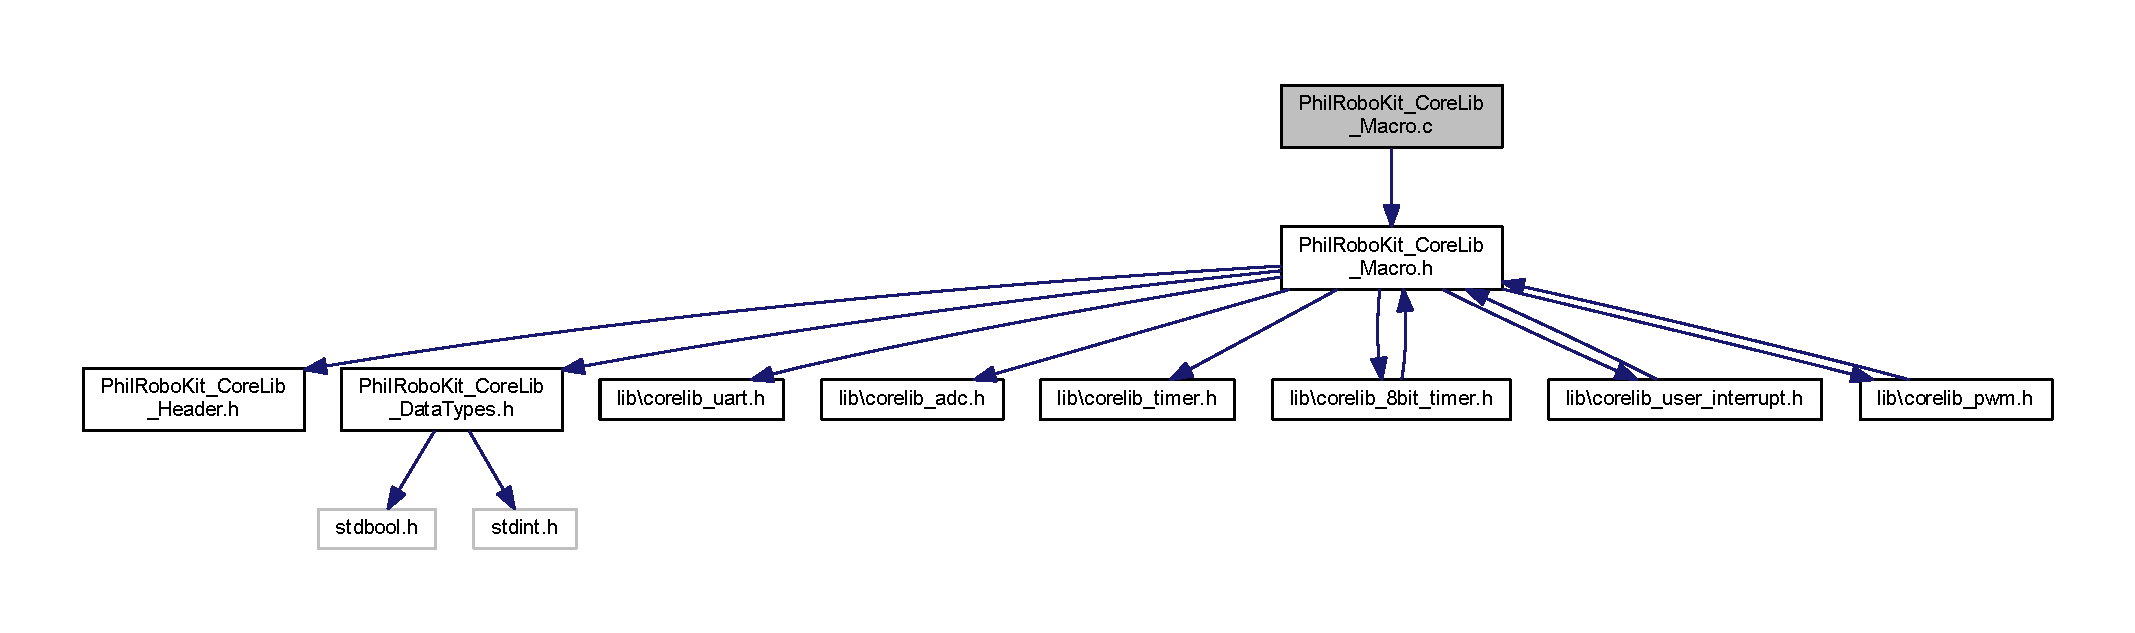
\includegraphics[width=350pt]{_phil_robo_kit___core_lib___macro_8c__incl}
\end{center}
\end{figure}
\subsection*{Functions}
\begin{DoxyCompactItemize}
\item 
{\bf \-\_\-\-\_\-\-C\-O\-N\-F\-I\-G} (W\-D\-T\-E\-\_\-\-O\-F\-F \&F\-O\-S\-C\-\_\-\-H\-S \&L\-V\-P\-\_\-\-O\-F\-F \&P\-W\-R\-T\-E\-\_\-\-O\-N \&B\-O\-R\-E\-N\-\_\-\-O\-F\-F)
\item 
void {\bf config\-Pin} (unsigned char uc\-Pin\-Name, char b\-Direction)
\item 
unsigned char {\bf check\-Pin\-State} (unsigned char uc\-Pin\-Name, char b\-Check\-State)
\item 
void {\bf philrobokit\-\_\-init} (void)
\item 
int {\bf main} (void)
\item 
void interrupt {\bf isr} (void)
\end{DoxyCompactItemize}


\subsection{Function Documentation}
\index{Phil\-Robo\-Kit\-\_\-\-Core\-Lib\-\_\-\-Macro.\-c@{Phil\-Robo\-Kit\-\_\-\-Core\-Lib\-\_\-\-Macro.\-c}!\-\_\-\-\_\-\-C\-O\-N\-F\-I\-G@{\-\_\-\-\_\-\-C\-O\-N\-F\-I\-G}}
\index{\-\_\-\-\_\-\-C\-O\-N\-F\-I\-G@{\-\_\-\-\_\-\-C\-O\-N\-F\-I\-G}!PhilRoboKit_CoreLib_Macro.c@{Phil\-Robo\-Kit\-\_\-\-Core\-Lib\-\_\-\-Macro.\-c}}
\subsubsection[{\-\_\-\-\_\-\-C\-O\-N\-F\-I\-G}]{\setlength{\rightskip}{0pt plus 5cm}\-\_\-\-\_\-\-C\-O\-N\-F\-I\-G (
\begin{DoxyParamCaption}
\item[{W\-D\-T\-E\-\_\-\-O\-F\-F \&F\-O\-S\-C\-\_\-\-H\-S \&L\-V\-P\-\_\-\-O\-F\-F \&P\-W\-R\-T\-E\-\_\-\-O\-N \&}]{B\-O\-R\-E\-N\-\_\-\-O\-F\-F}
\end{DoxyParamCaption}
)}\label{_phil_robo_kit___core_lib___macro_8c_a4515166f5bf82f6a7d9be7d8e9a4389b}
\index{Phil\-Robo\-Kit\-\_\-\-Core\-Lib\-\_\-\-Macro.\-c@{Phil\-Robo\-Kit\-\_\-\-Core\-Lib\-\_\-\-Macro.\-c}!check\-Pin\-State@{check\-Pin\-State}}
\index{check\-Pin\-State@{check\-Pin\-State}!PhilRoboKit_CoreLib_Macro.c@{Phil\-Robo\-Kit\-\_\-\-Core\-Lib\-\_\-\-Macro.\-c}}
\subsubsection[{check\-Pin\-State}]{\setlength{\rightskip}{0pt plus 5cm}unsigned char check\-Pin\-State (
\begin{DoxyParamCaption}
\item[{unsigned char}]{uc\-Pin\-Name, }
\item[{char}]{b\-Check\-State}
\end{DoxyParamCaption}
)}\label{_phil_robo_kit___core_lib___macro_8c_ac30b1018bb53a4641359277443ec47d1}


Definition at line 107 of file Phil\-Robo\-Kit\-\_\-\-Core\-Lib\-\_\-\-Macro.\-c.

\index{Phil\-Robo\-Kit\-\_\-\-Core\-Lib\-\_\-\-Macro.\-c@{Phil\-Robo\-Kit\-\_\-\-Core\-Lib\-\_\-\-Macro.\-c}!config\-Pin@{config\-Pin}}
\index{config\-Pin@{config\-Pin}!PhilRoboKit_CoreLib_Macro.c@{Phil\-Robo\-Kit\-\_\-\-Core\-Lib\-\_\-\-Macro.\-c}}
\subsubsection[{config\-Pin}]{\setlength{\rightskip}{0pt plus 5cm}void config\-Pin (
\begin{DoxyParamCaption}
\item[{unsigned char}]{uc\-Pin\-Name, }
\item[{char}]{b\-Direction}
\end{DoxyParamCaption}
)}\label{_phil_robo_kit___core_lib___macro_8c_a19923266a235ca6fea0783beec80ce2c}


Definition at line 46 of file Phil\-Robo\-Kit\-\_\-\-Core\-Lib\-\_\-\-Macro.\-c.

\index{Phil\-Robo\-Kit\-\_\-\-Core\-Lib\-\_\-\-Macro.\-c@{Phil\-Robo\-Kit\-\_\-\-Core\-Lib\-\_\-\-Macro.\-c}!isr@{isr}}
\index{isr@{isr}!PhilRoboKit_CoreLib_Macro.c@{Phil\-Robo\-Kit\-\_\-\-Core\-Lib\-\_\-\-Macro.\-c}}
\subsubsection[{isr}]{\setlength{\rightskip}{0pt plus 5cm}void interrupt isr (
\begin{DoxyParamCaption}
\item[{void}]{}
\end{DoxyParamCaption}
)}\label{_phil_robo_kit___core_lib___macro_8c_ad38f9db16d348bc4d2cb5ca91b5b575d}


Definition at line 243 of file Phil\-Robo\-Kit\-\_\-\-Core\-Lib\-\_\-\-Macro.\-c.



Here is the call graph for this function\-:\nopagebreak
\begin{figure}[H]
\begin{center}
\leavevmode
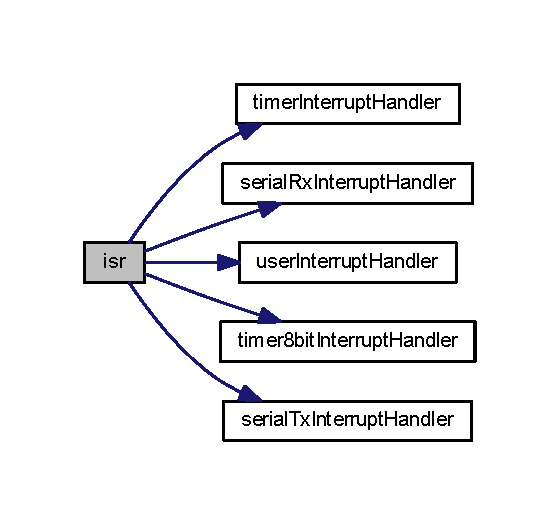
\includegraphics[width=268pt]{_phil_robo_kit___core_lib___macro_8c_ad38f9db16d348bc4d2cb5ca91b5b575d_cgraph}
\end{center}
\end{figure}


\index{Phil\-Robo\-Kit\-\_\-\-Core\-Lib\-\_\-\-Macro.\-c@{Phil\-Robo\-Kit\-\_\-\-Core\-Lib\-\_\-\-Macro.\-c}!main@{main}}
\index{main@{main}!PhilRoboKit_CoreLib_Macro.c@{Phil\-Robo\-Kit\-\_\-\-Core\-Lib\-\_\-\-Macro.\-c}}
\subsubsection[{main}]{\setlength{\rightskip}{0pt plus 5cm}int main (
\begin{DoxyParamCaption}
\item[{void}]{}
\end{DoxyParamCaption}
)}\label{_phil_robo_kit___core_lib___macro_8c_a840291bc02cba5474a4cb46a9b9566fe}


Definition at line 222 of file Phil\-Robo\-Kit\-\_\-\-Core\-Lib\-\_\-\-Macro.\-c.



Here is the call graph for this function\-:\nopagebreak
\begin{figure}[H]
\begin{center}
\leavevmode
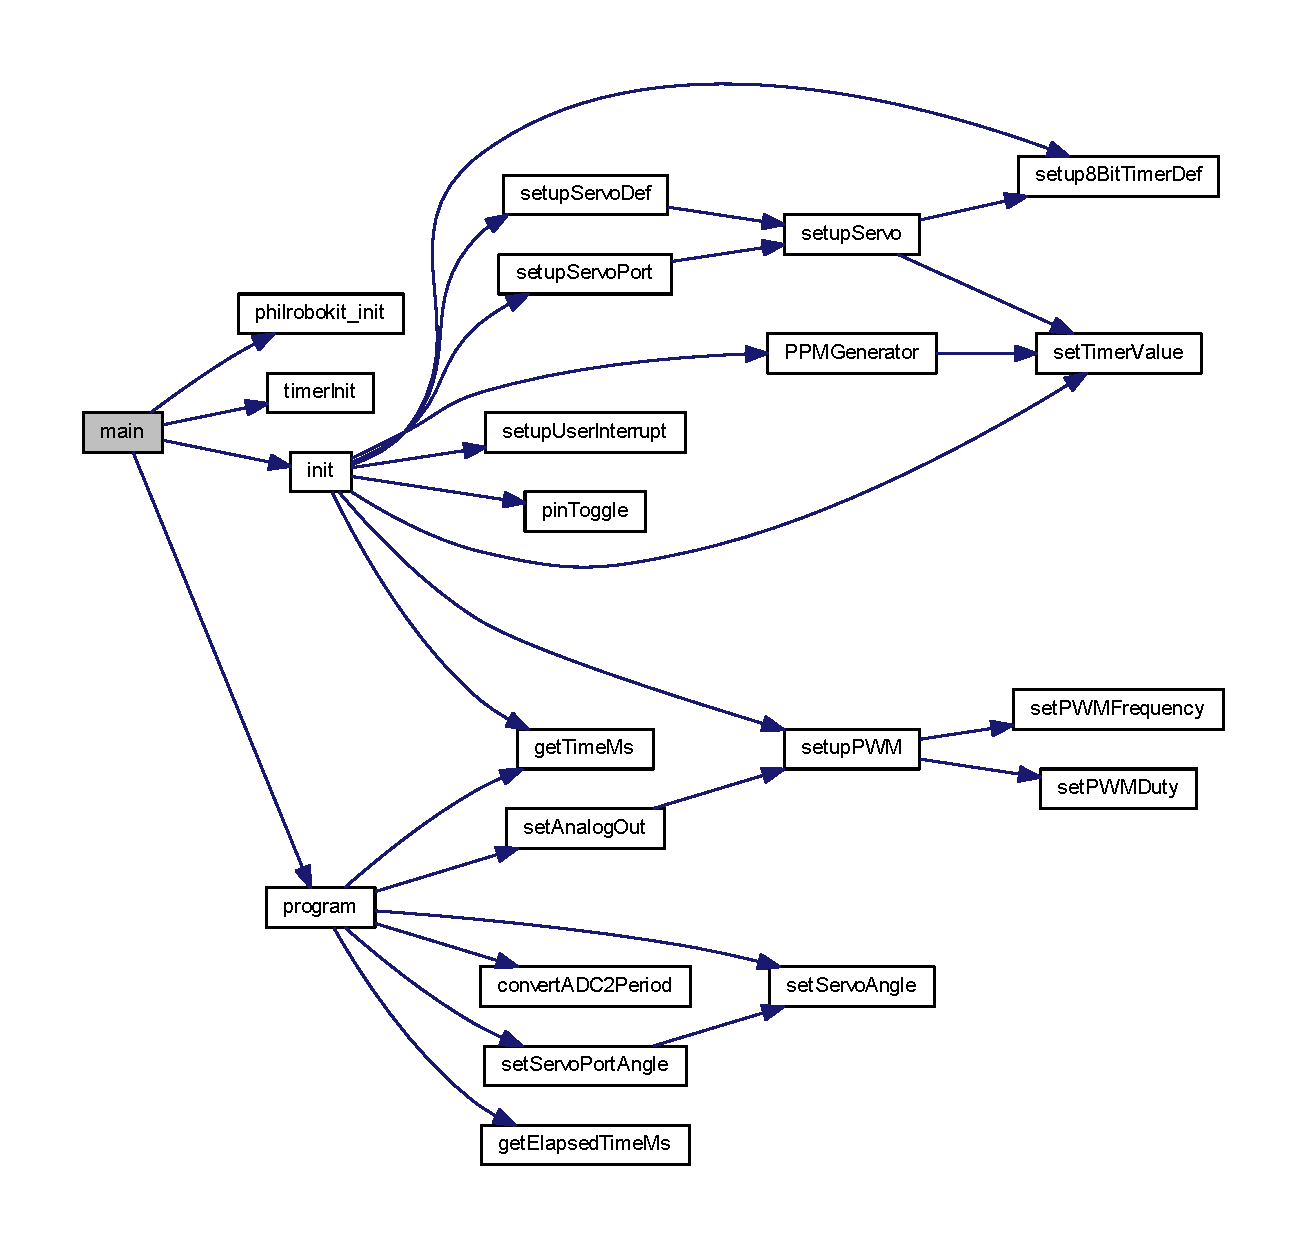
\includegraphics[width=350pt]{_phil_robo_kit___core_lib___macro_8c_a840291bc02cba5474a4cb46a9b9566fe_cgraph}
\end{center}
\end{figure}


\index{Phil\-Robo\-Kit\-\_\-\-Core\-Lib\-\_\-\-Macro.\-c@{Phil\-Robo\-Kit\-\_\-\-Core\-Lib\-\_\-\-Macro.\-c}!philrobokit\-\_\-init@{philrobokit\-\_\-init}}
\index{philrobokit\-\_\-init@{philrobokit\-\_\-init}!PhilRoboKit_CoreLib_Macro.c@{Phil\-Robo\-Kit\-\_\-\-Core\-Lib\-\_\-\-Macro.\-c}}
\subsubsection[{philrobokit\-\_\-init}]{\setlength{\rightskip}{0pt plus 5cm}void philrobokit\-\_\-init (
\begin{DoxyParamCaption}
\item[{void}]{}
\end{DoxyParamCaption}
)}\label{_phil_robo_kit___core_lib___macro_8c_abeecea64dc12504fc8236fdaeee3ae61}


Definition at line 210 of file Phil\-Robo\-Kit\-\_\-\-Core\-Lib\-\_\-\-Macro.\-c.


\section{Phil\-Robo\-Kit\-\_\-\-Core\-Lib\-\_\-\-Macro.\-h File Reference}
\label{_phil_robo_kit___core_lib___macro_8h}\index{Phil\-Robo\-Kit\-\_\-\-Core\-Lib\-\_\-\-Macro.\-h@{Phil\-Robo\-Kit\-\_\-\-Core\-Lib\-\_\-\-Macro.\-h}}
{\ttfamily \#include \char`\"{}Phil\-Robo\-Kit\-\_\-\-Core\-Lib\-\_\-\-Header.\-h\char`\"{}}\\*
{\ttfamily \#include \char`\"{}Phil\-Robo\-Kit\-\_\-\-Core\-Lib\-\_\-\-Data\-Types.\-h\char`\"{}}\\*
{\ttfamily \#include \char`\"{}lib\textbackslash{}corelib\-\_\-uart.\-h\char`\"{}}\\*
{\ttfamily \#include \char`\"{}lib\textbackslash{}corelib\-\_\-adc.\-h\char`\"{}}\\*
{\ttfamily \#include \char`\"{}lib\textbackslash{}corelib\-\_\-timer.\-h\char`\"{}}\\*
{\ttfamily \#include \char`\"{}lib\textbackslash{}corelib\-\_\-8bit\-\_\-timer.\-h\char`\"{}}\\*
{\ttfamily \#include \char`\"{}lib\textbackslash{}corelib\-\_\-user\-\_\-interrupt.\-h\char`\"{}}\\*
{\ttfamily \#include \char`\"{}lib\textbackslash{}corelib\-\_\-pwm.\-h\char`\"{}}\\*
Include dependency graph for Phil\-Robo\-Kit\-\_\-\-Core\-Lib\-\_\-\-Macro.\-h\-:\nopagebreak
\begin{figure}[H]
\begin{center}
\leavevmode
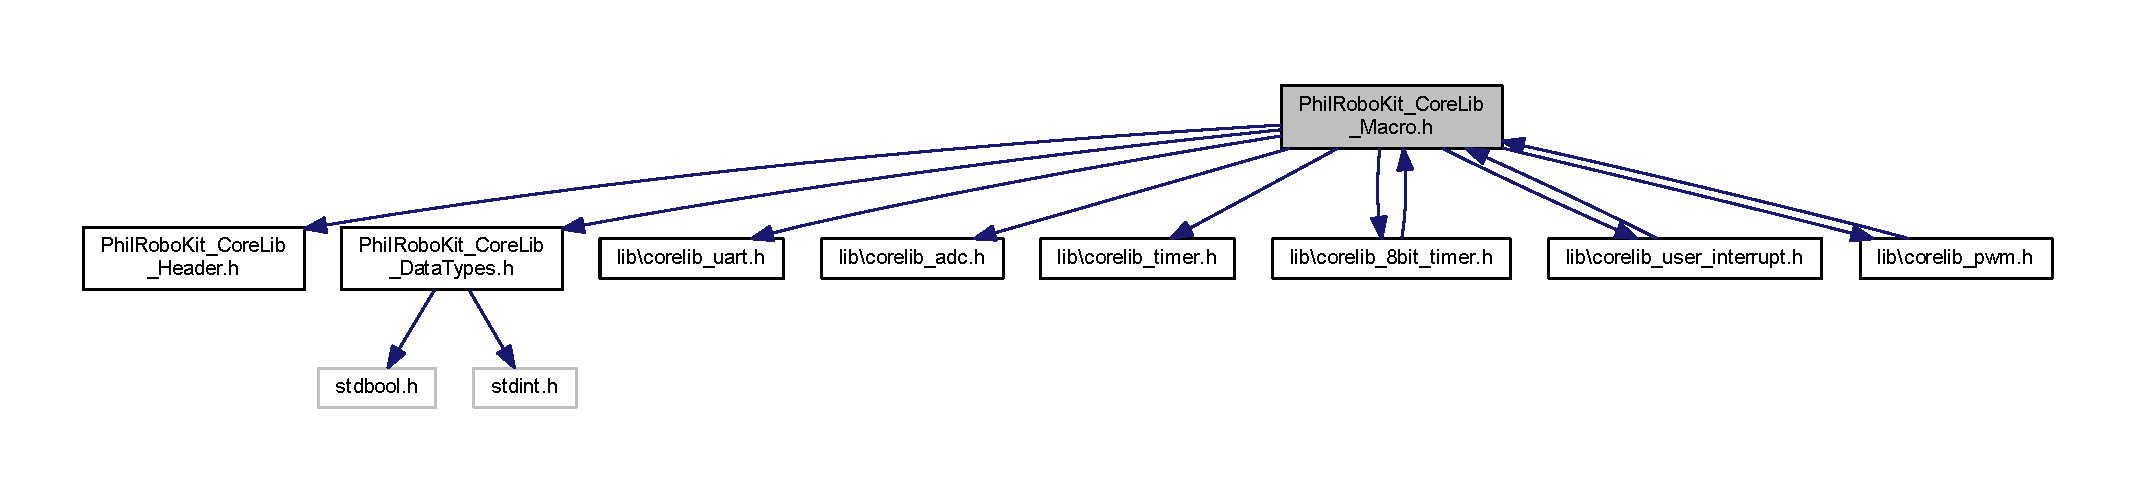
\includegraphics[width=350pt]{_phil_robo_kit___core_lib___macro_8h__incl}
\end{center}
\end{figure}
This graph shows which files directly or indirectly include this file\-:\nopagebreak
\begin{figure}[H]
\begin{center}
\leavevmode
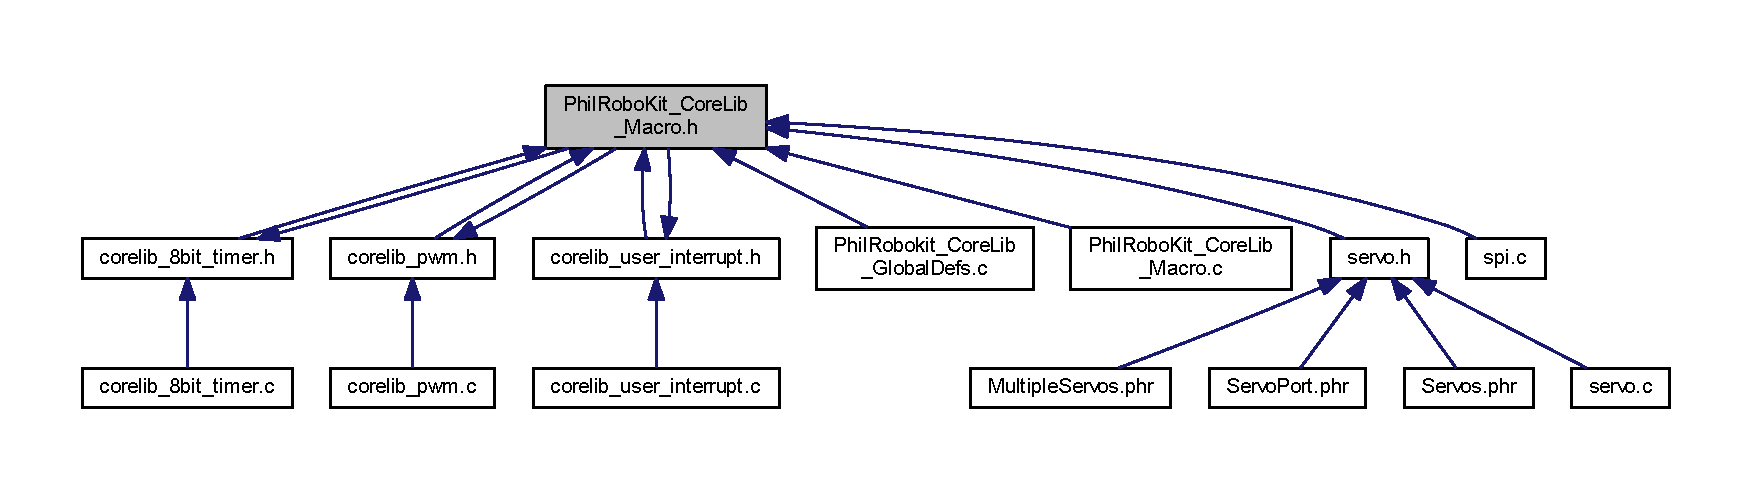
\includegraphics[width=350pt]{_phil_robo_kit___core_lib___macro_8h__dep__incl}
\end{center}
\end{figure}
\subsection*{Macros}
\begin{DoxyCompactItemize}
\item 
\#define {\bf I\-N}~1
\item 
\#define {\bf O\-U\-T}~0
\item 
\#define {\bf I\-N\-P\-U\-T}~{\bf I\-N}
\item 
\#define {\bf O\-U\-T\-P\-U\-T}~{\bf O\-U\-T}
\item 
\#define {\bf A\-N\-A\-L\-O\-G}~1
\item 
\#define {\bf H\-I\-G\-H}~1
\item 
\#define {\bf L\-O\-W}~0
\item 
\#define {\bf T\-R\-U\-E}~1
\item 
\#define {\bf F\-A\-L\-S\-E}~0
\item 
\#define {\bf set\-Pin}(x, y)~{\bf config\-Pin}(x,y)
\item 
\#define {\bf set\-Pin\-Input}(x)~{\bf config\-Pin}(x, {\bf I\-N})
\item 
\#define {\bf set\-Pin\-Output}(x)~{\bf config\-Pin}(x, {\bf O\-U\-T})
\item 
\#define {\bf set\-Pin\-High}(x)
\item 
\#define {\bf set\-Pin\-Low}(x)
\item 
\#define {\bf toggle\-Pin}(x)
\item 
\#define {\bf is\-Pin\-High}(x)~{\bf check\-Pin\-State}(x,{\bf H\-I\-G\-H})
\item 
\#define {\bf is\-Pin\-Low}(x)~{\bf check\-Pin\-State}(x,{\bf L\-O\-W})
\end{DoxyCompactItemize}
\subsection*{Functions}
\begin{DoxyCompactItemize}
\item 
void {\bf config\-Pin} (unsigned char uc\-Pin\-Name, char b\-Direction)
\item 
unsigned char {\bf check\-Pin\-State} (unsigned char uc\-Pin\-Name, char b\-Check\-State)
\item 
void {\bf timer\-Interrupt\-Handler} (void)
\item 
void {\bf user\-Interrupt\-Handler} (void)
\item 
void {\bf init} (void)
\item 
void {\bf program} (void)
\item 
void {\bf philrobokit\-\_\-init} (void)
\end{DoxyCompactItemize}


\subsection{Macro Definition Documentation}
\index{Phil\-Robo\-Kit\-\_\-\-Core\-Lib\-\_\-\-Macro.\-h@{Phil\-Robo\-Kit\-\_\-\-Core\-Lib\-\_\-\-Macro.\-h}!A\-N\-A\-L\-O\-G@{A\-N\-A\-L\-O\-G}}
\index{A\-N\-A\-L\-O\-G@{A\-N\-A\-L\-O\-G}!PhilRoboKit_CoreLib_Macro.h@{Phil\-Robo\-Kit\-\_\-\-Core\-Lib\-\_\-\-Macro.\-h}}
\subsubsection[{A\-N\-A\-L\-O\-G}]{\setlength{\rightskip}{0pt plus 5cm}\#define A\-N\-A\-L\-O\-G~1}\label{_phil_robo_kit___core_lib___macro_8h_ad42aa2404559d4a465d5d45e857f2881}


Definition at line 63 of file Phil\-Robo\-Kit\-\_\-\-Core\-Lib\-\_\-\-Macro.\-h.

\index{Phil\-Robo\-Kit\-\_\-\-Core\-Lib\-\_\-\-Macro.\-h@{Phil\-Robo\-Kit\-\_\-\-Core\-Lib\-\_\-\-Macro.\-h}!F\-A\-L\-S\-E@{F\-A\-L\-S\-E}}
\index{F\-A\-L\-S\-E@{F\-A\-L\-S\-E}!PhilRoboKit_CoreLib_Macro.h@{Phil\-Robo\-Kit\-\_\-\-Core\-Lib\-\_\-\-Macro.\-h}}
\subsubsection[{F\-A\-L\-S\-E}]{\setlength{\rightskip}{0pt plus 5cm}\#define F\-A\-L\-S\-E~0}\label{_phil_robo_kit___core_lib___macro_8h_aa93f0eb578d23995850d61f7d61c55c1}


Definition at line 69 of file Phil\-Robo\-Kit\-\_\-\-Core\-Lib\-\_\-\-Macro.\-h.

\index{Phil\-Robo\-Kit\-\_\-\-Core\-Lib\-\_\-\-Macro.\-h@{Phil\-Robo\-Kit\-\_\-\-Core\-Lib\-\_\-\-Macro.\-h}!H\-I\-G\-H@{H\-I\-G\-H}}
\index{H\-I\-G\-H@{H\-I\-G\-H}!PhilRoboKit_CoreLib_Macro.h@{Phil\-Robo\-Kit\-\_\-\-Core\-Lib\-\_\-\-Macro.\-h}}
\subsubsection[{H\-I\-G\-H}]{\setlength{\rightskip}{0pt plus 5cm}\#define H\-I\-G\-H~1}\label{_phil_robo_kit___core_lib___macro_8h_a5bb885982ff66a2e0a0a45a8ee9c35e2}


Definition at line 65 of file Phil\-Robo\-Kit\-\_\-\-Core\-Lib\-\_\-\-Macro.\-h.

\index{Phil\-Robo\-Kit\-\_\-\-Core\-Lib\-\_\-\-Macro.\-h@{Phil\-Robo\-Kit\-\_\-\-Core\-Lib\-\_\-\-Macro.\-h}!I\-N@{I\-N}}
\index{I\-N@{I\-N}!PhilRoboKit_CoreLib_Macro.h@{Phil\-Robo\-Kit\-\_\-\-Core\-Lib\-\_\-\-Macro.\-h}}
\subsubsection[{I\-N}]{\setlength{\rightskip}{0pt plus 5cm}\#define I\-N~1}\label{_phil_robo_kit___core_lib___macro_8h_ac2bbd6d630a06a980d9a92ddb9a49928}


Definition at line 58 of file Phil\-Robo\-Kit\-\_\-\-Core\-Lib\-\_\-\-Macro.\-h.

\index{Phil\-Robo\-Kit\-\_\-\-Core\-Lib\-\_\-\-Macro.\-h@{Phil\-Robo\-Kit\-\_\-\-Core\-Lib\-\_\-\-Macro.\-h}!I\-N\-P\-U\-T@{I\-N\-P\-U\-T}}
\index{I\-N\-P\-U\-T@{I\-N\-P\-U\-T}!PhilRoboKit_CoreLib_Macro.h@{Phil\-Robo\-Kit\-\_\-\-Core\-Lib\-\_\-\-Macro.\-h}}
\subsubsection[{I\-N\-P\-U\-T}]{\setlength{\rightskip}{0pt plus 5cm}\#define I\-N\-P\-U\-T~{\bf I\-N}}\label{_phil_robo_kit___core_lib___macro_8h_a1bb283bd7893b9855e2f23013891fc82}


Definition at line 61 of file Phil\-Robo\-Kit\-\_\-\-Core\-Lib\-\_\-\-Macro.\-h.

\index{Phil\-Robo\-Kit\-\_\-\-Core\-Lib\-\_\-\-Macro.\-h@{Phil\-Robo\-Kit\-\_\-\-Core\-Lib\-\_\-\-Macro.\-h}!is\-Pin\-High@{is\-Pin\-High}}
\index{is\-Pin\-High@{is\-Pin\-High}!PhilRoboKit_CoreLib_Macro.h@{Phil\-Robo\-Kit\-\_\-\-Core\-Lib\-\_\-\-Macro.\-h}}
\subsubsection[{is\-Pin\-High}]{\setlength{\rightskip}{0pt plus 5cm}\#define is\-Pin\-High(
\begin{DoxyParamCaption}
\item[{}]{x}
\end{DoxyParamCaption}
)~{\bf check\-Pin\-State}(x,{\bf H\-I\-G\-H})}\label{_phil_robo_kit___core_lib___macro_8h_a05d0b3e17ba8edfe3653898f0b86350f}


Definition at line 103 of file Phil\-Robo\-Kit\-\_\-\-Core\-Lib\-\_\-\-Macro.\-h.

\index{Phil\-Robo\-Kit\-\_\-\-Core\-Lib\-\_\-\-Macro.\-h@{Phil\-Robo\-Kit\-\_\-\-Core\-Lib\-\_\-\-Macro.\-h}!is\-Pin\-Low@{is\-Pin\-Low}}
\index{is\-Pin\-Low@{is\-Pin\-Low}!PhilRoboKit_CoreLib_Macro.h@{Phil\-Robo\-Kit\-\_\-\-Core\-Lib\-\_\-\-Macro.\-h}}
\subsubsection[{is\-Pin\-Low}]{\setlength{\rightskip}{0pt plus 5cm}\#define is\-Pin\-Low(
\begin{DoxyParamCaption}
\item[{}]{x}
\end{DoxyParamCaption}
)~{\bf check\-Pin\-State}(x,{\bf L\-O\-W})}\label{_phil_robo_kit___core_lib___macro_8h_a4dcb01d02bd94957e9f096df78162afd}


Definition at line 104 of file Phil\-Robo\-Kit\-\_\-\-Core\-Lib\-\_\-\-Macro.\-h.

\index{Phil\-Robo\-Kit\-\_\-\-Core\-Lib\-\_\-\-Macro.\-h@{Phil\-Robo\-Kit\-\_\-\-Core\-Lib\-\_\-\-Macro.\-h}!L\-O\-W@{L\-O\-W}}
\index{L\-O\-W@{L\-O\-W}!PhilRoboKit_CoreLib_Macro.h@{Phil\-Robo\-Kit\-\_\-\-Core\-Lib\-\_\-\-Macro.\-h}}
\subsubsection[{L\-O\-W}]{\setlength{\rightskip}{0pt plus 5cm}\#define L\-O\-W~0}\label{_phil_robo_kit___core_lib___macro_8h_ab811d8c6ff3a505312d3276590444289}


Definition at line 66 of file Phil\-Robo\-Kit\-\_\-\-Core\-Lib\-\_\-\-Macro.\-h.

\index{Phil\-Robo\-Kit\-\_\-\-Core\-Lib\-\_\-\-Macro.\-h@{Phil\-Robo\-Kit\-\_\-\-Core\-Lib\-\_\-\-Macro.\-h}!O\-U\-T@{O\-U\-T}}
\index{O\-U\-T@{O\-U\-T}!PhilRoboKit_CoreLib_Macro.h@{Phil\-Robo\-Kit\-\_\-\-Core\-Lib\-\_\-\-Macro.\-h}}
\subsubsection[{O\-U\-T}]{\setlength{\rightskip}{0pt plus 5cm}\#define O\-U\-T~0}\label{_phil_robo_kit___core_lib___macro_8h_aec78e7a9e90a406a56f859ee456e8eae}


Definition at line 59 of file Phil\-Robo\-Kit\-\_\-\-Core\-Lib\-\_\-\-Macro.\-h.

\index{Phil\-Robo\-Kit\-\_\-\-Core\-Lib\-\_\-\-Macro.\-h@{Phil\-Robo\-Kit\-\_\-\-Core\-Lib\-\_\-\-Macro.\-h}!O\-U\-T\-P\-U\-T@{O\-U\-T\-P\-U\-T}}
\index{O\-U\-T\-P\-U\-T@{O\-U\-T\-P\-U\-T}!PhilRoboKit_CoreLib_Macro.h@{Phil\-Robo\-Kit\-\_\-\-Core\-Lib\-\_\-\-Macro.\-h}}
\subsubsection[{O\-U\-T\-P\-U\-T}]{\setlength{\rightskip}{0pt plus 5cm}\#define O\-U\-T\-P\-U\-T~{\bf O\-U\-T}}\label{_phil_robo_kit___core_lib___macro_8h_a61a3c9a18380aafb6e430e79bf596557}


Definition at line 62 of file Phil\-Robo\-Kit\-\_\-\-Core\-Lib\-\_\-\-Macro.\-h.

\index{Phil\-Robo\-Kit\-\_\-\-Core\-Lib\-\_\-\-Macro.\-h@{Phil\-Robo\-Kit\-\_\-\-Core\-Lib\-\_\-\-Macro.\-h}!set\-Pin@{set\-Pin}}
\index{set\-Pin@{set\-Pin}!PhilRoboKit_CoreLib_Macro.h@{Phil\-Robo\-Kit\-\_\-\-Core\-Lib\-\_\-\-Macro.\-h}}
\subsubsection[{set\-Pin}]{\setlength{\rightskip}{0pt plus 5cm}\#define set\-Pin(
\begin{DoxyParamCaption}
\item[{}]{x, }
\item[{}]{y}
\end{DoxyParamCaption}
)~{\bf config\-Pin}(x,y)}\label{_phil_robo_kit___core_lib___macro_8h_a6a9342ef97a53f118bdc973d3ffb1e91}


Definition at line 71 of file Phil\-Robo\-Kit\-\_\-\-Core\-Lib\-\_\-\-Macro.\-h.

\index{Phil\-Robo\-Kit\-\_\-\-Core\-Lib\-\_\-\-Macro.\-h@{Phil\-Robo\-Kit\-\_\-\-Core\-Lib\-\_\-\-Macro.\-h}!set\-Pin\-High@{set\-Pin\-High}}
\index{set\-Pin\-High@{set\-Pin\-High}!PhilRoboKit_CoreLib_Macro.h@{Phil\-Robo\-Kit\-\_\-\-Core\-Lib\-\_\-\-Macro.\-h}}
\subsubsection[{set\-Pin\-High}]{\setlength{\rightskip}{0pt plus 5cm}\#define set\-Pin\-High(
\begin{DoxyParamCaption}
\item[{}]{x}
\end{DoxyParamCaption}
)}\label{_phil_robo_kit___core_lib___macro_8h_a2eda14a8d2a7c56022748cbc90c9ab00}
{\bfseries Value\-:}
\begin{DoxyCode}
\{ \(\backslash\)
     if(x<=7) \{ \(\backslash\)
          REGISTER\_PORTC |= (1UL<<x); \(\backslash\)
     \}\textcolor{keywordflow}{else} \textcolor{keywordflow}{if}(x>=8 && x<=13) \{ \(\backslash\)
          REGISTER\_PORTB |= (1UL<<(x-8)); \(\backslash\)
     \}\textcolor{keywordflow}{else} \textcolor{keywordflow}{if}(x>=21 && x<=28) \{ \(\backslash\)
          REGISTER\_PORTD |= (1UL<<(x-21)); \(\backslash\)
     \} \(\backslash\)
\}
\end{DoxyCode}


Definition at line 75 of file Phil\-Robo\-Kit\-\_\-\-Core\-Lib\-\_\-\-Macro.\-h.

\index{Phil\-Robo\-Kit\-\_\-\-Core\-Lib\-\_\-\-Macro.\-h@{Phil\-Robo\-Kit\-\_\-\-Core\-Lib\-\_\-\-Macro.\-h}!set\-Pin\-Input@{set\-Pin\-Input}}
\index{set\-Pin\-Input@{set\-Pin\-Input}!PhilRoboKit_CoreLib_Macro.h@{Phil\-Robo\-Kit\-\_\-\-Core\-Lib\-\_\-\-Macro.\-h}}
\subsubsection[{set\-Pin\-Input}]{\setlength{\rightskip}{0pt plus 5cm}\#define set\-Pin\-Input(
\begin{DoxyParamCaption}
\item[{}]{x}
\end{DoxyParamCaption}
)~{\bf config\-Pin}(x, {\bf I\-N})}\label{_phil_robo_kit___core_lib___macro_8h_a1426e7826729d8875aeba7a0e2b6a217}


Definition at line 72 of file Phil\-Robo\-Kit\-\_\-\-Core\-Lib\-\_\-\-Macro.\-h.

\index{Phil\-Robo\-Kit\-\_\-\-Core\-Lib\-\_\-\-Macro.\-h@{Phil\-Robo\-Kit\-\_\-\-Core\-Lib\-\_\-\-Macro.\-h}!set\-Pin\-Low@{set\-Pin\-Low}}
\index{set\-Pin\-Low@{set\-Pin\-Low}!PhilRoboKit_CoreLib_Macro.h@{Phil\-Robo\-Kit\-\_\-\-Core\-Lib\-\_\-\-Macro.\-h}}
\subsubsection[{set\-Pin\-Low}]{\setlength{\rightskip}{0pt plus 5cm}\#define set\-Pin\-Low(
\begin{DoxyParamCaption}
\item[{}]{x}
\end{DoxyParamCaption}
)}\label{_phil_robo_kit___core_lib___macro_8h_ae77921bdc97c16d3cbe59bf31d1e3885}
{\bfseries Value\-:}
\begin{DoxyCode}
\{ \(\backslash\)
     if(x<=7) \{ \(\backslash\)
          REGISTER\_PORTC &= ~(1UL<<x); \(\backslash\)
     \}\textcolor{keywordflow}{else} \textcolor{keywordflow}{if}(x>=8 && x<=13) \{ \(\backslash\)
          REGISTER\_PORTB &= ~(1UL<<(x-8)); \(\backslash\)
     \}\textcolor{keywordflow}{else} \textcolor{keywordflow}{if}(x>=21 && x<=28) \{ \(\backslash\)
          REGISTER\_PORTD &= ~(1UL<<(x-21)); \(\backslash\)
     \} \(\backslash\)
\}
\end{DoxyCode}


Definition at line 84 of file Phil\-Robo\-Kit\-\_\-\-Core\-Lib\-\_\-\-Macro.\-h.

\index{Phil\-Robo\-Kit\-\_\-\-Core\-Lib\-\_\-\-Macro.\-h@{Phil\-Robo\-Kit\-\_\-\-Core\-Lib\-\_\-\-Macro.\-h}!set\-Pin\-Output@{set\-Pin\-Output}}
\index{set\-Pin\-Output@{set\-Pin\-Output}!PhilRoboKit_CoreLib_Macro.h@{Phil\-Robo\-Kit\-\_\-\-Core\-Lib\-\_\-\-Macro.\-h}}
\subsubsection[{set\-Pin\-Output}]{\setlength{\rightskip}{0pt plus 5cm}\#define set\-Pin\-Output(
\begin{DoxyParamCaption}
\item[{}]{x}
\end{DoxyParamCaption}
)~{\bf config\-Pin}(x, {\bf O\-U\-T})}\label{_phil_robo_kit___core_lib___macro_8h_a38d4d2f9c5196b8e2b027fa33b0770ac}


Definition at line 73 of file Phil\-Robo\-Kit\-\_\-\-Core\-Lib\-\_\-\-Macro.\-h.

\index{Phil\-Robo\-Kit\-\_\-\-Core\-Lib\-\_\-\-Macro.\-h@{Phil\-Robo\-Kit\-\_\-\-Core\-Lib\-\_\-\-Macro.\-h}!toggle\-Pin@{toggle\-Pin}}
\index{toggle\-Pin@{toggle\-Pin}!PhilRoboKit_CoreLib_Macro.h@{Phil\-Robo\-Kit\-\_\-\-Core\-Lib\-\_\-\-Macro.\-h}}
\subsubsection[{toggle\-Pin}]{\setlength{\rightskip}{0pt plus 5cm}\#define toggle\-Pin(
\begin{DoxyParamCaption}
\item[{}]{x}
\end{DoxyParamCaption}
)}\label{_phil_robo_kit___core_lib___macro_8h_ab278de2f52559384724741a48cb71ca7}
{\bfseries Value\-:}
\begin{DoxyCode}
\{ \(\backslash\)
     if(x<=7) \{ \(\backslash\)
          REGISTER\_PORTC ^= (1UL<<x); \(\backslash\)
     \}\textcolor{keywordflow}{else} \textcolor{keywordflow}{if} (x>=8 && x<=13) \{ \(\backslash\)
          REGISTER\_PORTB ^= (1UL<<(x-8)); \(\backslash\)
     \}\textcolor{keywordflow}{else} \textcolor{keywordflow}{if}(x>=21 && x<=28) \{ \(\backslash\)
          REGISTER\_PORTD ^= (1UL<<(x-21)); \(\backslash\)
     \} \(\backslash\)
\}
\end{DoxyCode}


Definition at line 93 of file Phil\-Robo\-Kit\-\_\-\-Core\-Lib\-\_\-\-Macro.\-h.

\index{Phil\-Robo\-Kit\-\_\-\-Core\-Lib\-\_\-\-Macro.\-h@{Phil\-Robo\-Kit\-\_\-\-Core\-Lib\-\_\-\-Macro.\-h}!T\-R\-U\-E@{T\-R\-U\-E}}
\index{T\-R\-U\-E@{T\-R\-U\-E}!PhilRoboKit_CoreLib_Macro.h@{Phil\-Robo\-Kit\-\_\-\-Core\-Lib\-\_\-\-Macro.\-h}}
\subsubsection[{T\-R\-U\-E}]{\setlength{\rightskip}{0pt plus 5cm}\#define T\-R\-U\-E~1}\label{_phil_robo_kit___core_lib___macro_8h_aa8cecfc5c5c054d2875c03e77b7be15d}


Definition at line 68 of file Phil\-Robo\-Kit\-\_\-\-Core\-Lib\-\_\-\-Macro.\-h.



\subsection{Function Documentation}
\index{Phil\-Robo\-Kit\-\_\-\-Core\-Lib\-\_\-\-Macro.\-h@{Phil\-Robo\-Kit\-\_\-\-Core\-Lib\-\_\-\-Macro.\-h}!check\-Pin\-State@{check\-Pin\-State}}
\index{check\-Pin\-State@{check\-Pin\-State}!PhilRoboKit_CoreLib_Macro.h@{Phil\-Robo\-Kit\-\_\-\-Core\-Lib\-\_\-\-Macro.\-h}}
\subsubsection[{check\-Pin\-State}]{\setlength{\rightskip}{0pt plus 5cm}unsigned char check\-Pin\-State (
\begin{DoxyParamCaption}
\item[{unsigned char}]{uc\-Pin\-Name, }
\item[{char}]{b\-Check\-State}
\end{DoxyParamCaption}
)}\label{_phil_robo_kit___core_lib___macro_8h_ac30b1018bb53a4641359277443ec47d1}


Definition at line 107 of file Phil\-Robo\-Kit\-\_\-\-Core\-Lib\-\_\-\-Macro.\-c.

\index{Phil\-Robo\-Kit\-\_\-\-Core\-Lib\-\_\-\-Macro.\-h@{Phil\-Robo\-Kit\-\_\-\-Core\-Lib\-\_\-\-Macro.\-h}!config\-Pin@{config\-Pin}}
\index{config\-Pin@{config\-Pin}!PhilRoboKit_CoreLib_Macro.h@{Phil\-Robo\-Kit\-\_\-\-Core\-Lib\-\_\-\-Macro.\-h}}
\subsubsection[{config\-Pin}]{\setlength{\rightskip}{0pt plus 5cm}void config\-Pin (
\begin{DoxyParamCaption}
\item[{unsigned char}]{uc\-Pin\-Name, }
\item[{char}]{b\-Direction}
\end{DoxyParamCaption}
)}\label{_phil_robo_kit___core_lib___macro_8h_a19923266a235ca6fea0783beec80ce2c}


Definition at line 46 of file Phil\-Robo\-Kit\-\_\-\-Core\-Lib\-\_\-\-Macro.\-c.

\index{Phil\-Robo\-Kit\-\_\-\-Core\-Lib\-\_\-\-Macro.\-h@{Phil\-Robo\-Kit\-\_\-\-Core\-Lib\-\_\-\-Macro.\-h}!init@{init}}
\index{init@{init}!PhilRoboKit_CoreLib_Macro.h@{Phil\-Robo\-Kit\-\_\-\-Core\-Lib\-\_\-\-Macro.\-h}}
\subsubsection[{init}]{\setlength{\rightskip}{0pt plus 5cm}void init (
\begin{DoxyParamCaption}
\item[{void}]{}
\end{DoxyParamCaption}
)}\label{_phil_robo_kit___core_lib___macro_8h_a2858154e2009b0e6e616f313177762bc}


Definition at line 17 of file Blink\-Without\-Delay.\-phr.



Here is the call graph for this function\-:\nopagebreak
\begin{figure}[H]
\begin{center}
\leavevmode
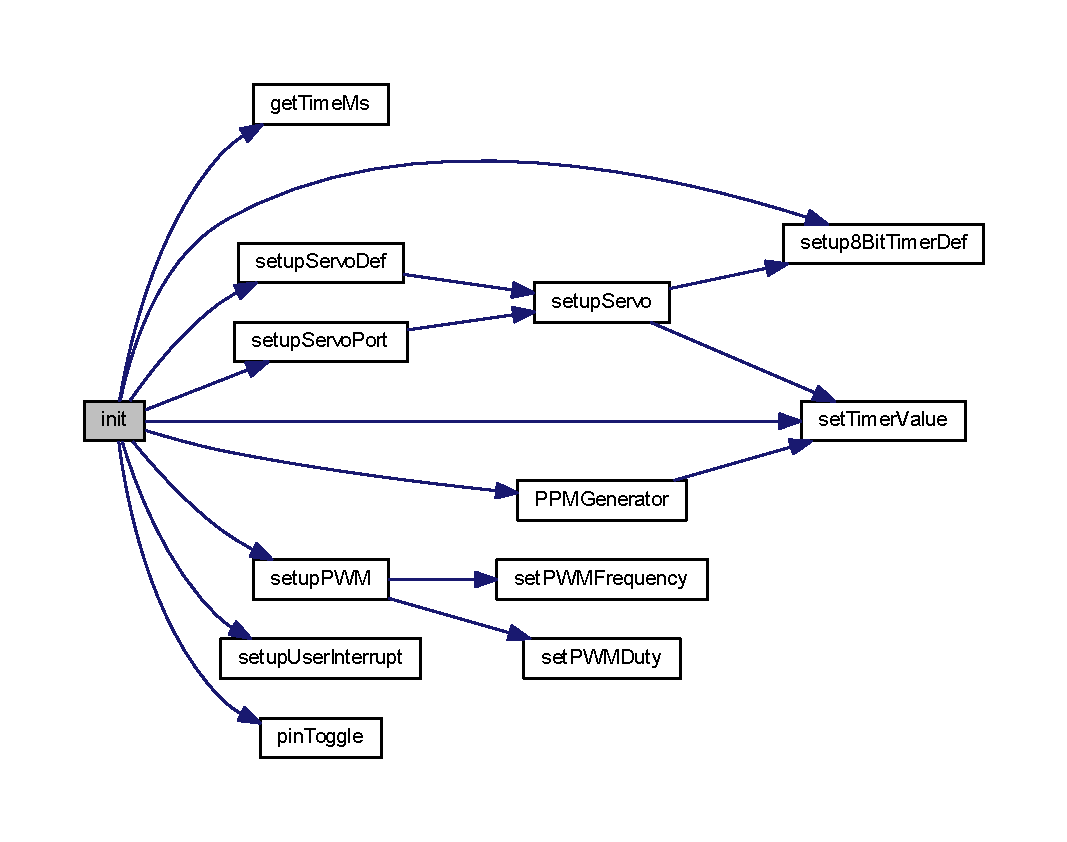
\includegraphics[width=350pt]{_phil_robo_kit___core_lib___macro_8h_a2858154e2009b0e6e616f313177762bc_cgraph}
\end{center}
\end{figure}


\index{Phil\-Robo\-Kit\-\_\-\-Core\-Lib\-\_\-\-Macro.\-h@{Phil\-Robo\-Kit\-\_\-\-Core\-Lib\-\_\-\-Macro.\-h}!philrobokit\-\_\-init@{philrobokit\-\_\-init}}
\index{philrobokit\-\_\-init@{philrobokit\-\_\-init}!PhilRoboKit_CoreLib_Macro.h@{Phil\-Robo\-Kit\-\_\-\-Core\-Lib\-\_\-\-Macro.\-h}}
\subsubsection[{philrobokit\-\_\-init}]{\setlength{\rightskip}{0pt plus 5cm}void philrobokit\-\_\-init (
\begin{DoxyParamCaption}
\item[{void}]{}
\end{DoxyParamCaption}
)}\label{_phil_robo_kit___core_lib___macro_8h_abeecea64dc12504fc8236fdaeee3ae61}


Definition at line 210 of file Phil\-Robo\-Kit\-\_\-\-Core\-Lib\-\_\-\-Macro.\-c.

\index{Phil\-Robo\-Kit\-\_\-\-Core\-Lib\-\_\-\-Macro.\-h@{Phil\-Robo\-Kit\-\_\-\-Core\-Lib\-\_\-\-Macro.\-h}!program@{program}}
\index{program@{program}!PhilRoboKit_CoreLib_Macro.h@{Phil\-Robo\-Kit\-\_\-\-Core\-Lib\-\_\-\-Macro.\-h}}
\subsubsection[{program}]{\setlength{\rightskip}{0pt plus 5cm}void program (
\begin{DoxyParamCaption}
\item[{void}]{}
\end{DoxyParamCaption}
)}\label{_phil_robo_kit___core_lib___macro_8h_a4e60091b55013a9208e1f53f8bc391c9}


Definition at line 27 of file Blink\-Without\-Delay.\-phr.



Here is the call graph for this function\-:\nopagebreak
\begin{figure}[H]
\begin{center}
\leavevmode
\includegraphics[width=350pt]{_phil_robo_kit___core_lib___macro_8h_a4e60091b55013a9208e1f53f8bc391c9_cgraph}
\end{center}
\end{figure}


\index{Phil\-Robo\-Kit\-\_\-\-Core\-Lib\-\_\-\-Macro.\-h@{Phil\-Robo\-Kit\-\_\-\-Core\-Lib\-\_\-\-Macro.\-h}!timer\-Interrupt\-Handler@{timer\-Interrupt\-Handler}}
\index{timer\-Interrupt\-Handler@{timer\-Interrupt\-Handler}!PhilRoboKit_CoreLib_Macro.h@{Phil\-Robo\-Kit\-\_\-\-Core\-Lib\-\_\-\-Macro.\-h}}
\subsubsection[{timer\-Interrupt\-Handler}]{\setlength{\rightskip}{0pt plus 5cm}void timer\-Interrupt\-Handler (
\begin{DoxyParamCaption}
\item[{void}]{}
\end{DoxyParamCaption}
)}\label{_phil_robo_kit___core_lib___macro_8h_ae6b9991ee92a30ad115ef6928829566a}


Definition at line 39 of file corelib\-\_\-timer.\-c.

\index{Phil\-Robo\-Kit\-\_\-\-Core\-Lib\-\_\-\-Macro.\-h@{Phil\-Robo\-Kit\-\_\-\-Core\-Lib\-\_\-\-Macro.\-h}!user\-Interrupt\-Handler@{user\-Interrupt\-Handler}}
\index{user\-Interrupt\-Handler@{user\-Interrupt\-Handler}!PhilRoboKit_CoreLib_Macro.h@{Phil\-Robo\-Kit\-\_\-\-Core\-Lib\-\_\-\-Macro.\-h}}
\subsubsection[{user\-Interrupt\-Handler}]{\setlength{\rightskip}{0pt plus 5cm}void user\-Interrupt\-Handler (
\begin{DoxyParamCaption}
\item[{void}]{}
\end{DoxyParamCaption}
)}\label{_phil_robo_kit___core_lib___macro_8h_aa1ef5be24251d01808e5dec4c6babd01}


Definition at line 178 of file corelib\-\_\-user\-\_\-interrupt.\-c.


\section{P\-P\-M\-Generator.\-phr File Reference}
\label{_p_p_m_generator_8phr}\index{P\-P\-M\-Generator.\-phr@{P\-P\-M\-Generator.\-phr}}
\subsection*{Macros}
\begin{DoxyCompactItemize}
\item 
\#define {\bf N\-U\-M\-\_\-\-O\-F\-\_\-\-C\-H\-A\-N\-N\-E\-L\-S}~6
\item 
\#define {\bf T\-M\-R2\-\_\-\-M\-A\-X\-\_\-\-C\-O\-U\-N\-T}~255
\item 
\#define {\bf P\-U\-L\-S\-E\-\_\-\-P\-E\-R\-I\-O\-D}~15
\item 
\#define {\bf C\-Y\-C\-L\-E\-\_\-\-P\-E\-R\-I\-O\-D}~2500
\item 
\#define {\bf M\-A\-X\-\_\-\-P\-O\-S\-I\-T\-I\-O\-N}~250
\item 
\#define {\bf D\-E\-F\-\_\-\-P\-O\-S\-I\-T\-I\-O\-N}~150
\item 
\#define {\bf M\-I\-N\-\_\-\-P\-O\-S\-I\-T\-I\-O\-N}~50
\item 
\#define {\bf A\-D\-C2\-P\-P\-M\-\_\-\-S\-L\-O\-P\-E}~((250-\/50)$\ast$256/(1023))
\item 
\#define {\bf A\-D\-C2\-P\-P\-M\-\_\-\-O\-F\-F\-S\-E\-T}~{\bf D\-E\-F\-\_\-\-P\-O\-S\-I\-T\-I\-O\-N}
\end{DoxyCompactItemize}
\subsection*{Enumerations}
\begin{DoxyCompactItemize}
\item 
enum {\bf P\-P\-M\-Gen\-States} \{ {\bf S\-E\-N\-D\-\_\-\-P\-U\-L\-S\-E}, 
{\bf S\-E\-N\-D\-\_\-\-C\-H\-A\-N\-N\-E\-L\-\_\-\-P\-E\-R\-I\-O\-D}, 
{\bf W\-A\-I\-T\-\_\-\-E\-N\-D\-\_\-\-O\-F\-\_\-\-C\-Y\-C\-L\-E}
 \}
\end{DoxyCompactItemize}
\subsection*{Functions}
\begin{DoxyCompactItemize}
\item 
void {\bf P\-P\-M\-Generator} ()
\item 
unsigned int {\bf convert\-A\-D\-C2\-Period} (unsigned int A\-D\-C\-Value)
\item 
void {\bf init} ()
\item 
void {\bf program} ()
\end{DoxyCompactItemize}
\subsection*{Variables}
\begin{DoxyCompactItemize}
\item 
unsigned char {\bf Channel\-Periods} [{\bf N\-U\-M\-\_\-\-O\-F\-\_\-\-C\-H\-A\-N\-N\-E\-L\-S}]
\item 
unsigned char {\bf P\-P\-M\-\_\-\-State}
\item 
unsigned char {\bf tempvar}
\item 
signed char {\bf channel\-\_\-ctr}
\item 
unsigned long {\bf Frame\-Blank\-Time}
\item 
unsigned long {\bf Sum\-Of\-Periods}
\item 
bit\-\_\-t {\bf Send\-Pulse}
\item 
bit\-\_\-t {\bf Blank\-Time\-Set}
\end{DoxyCompactItemize}


\subsection{Macro Definition Documentation}
\index{P\-P\-M\-Generator.\-phr@{P\-P\-M\-Generator.\-phr}!A\-D\-C2\-P\-P\-M\-\_\-\-O\-F\-F\-S\-E\-T@{A\-D\-C2\-P\-P\-M\-\_\-\-O\-F\-F\-S\-E\-T}}
\index{A\-D\-C2\-P\-P\-M\-\_\-\-O\-F\-F\-S\-E\-T@{A\-D\-C2\-P\-P\-M\-\_\-\-O\-F\-F\-S\-E\-T}!PPMGenerator.phr@{P\-P\-M\-Generator.\-phr}}
\subsubsection[{A\-D\-C2\-P\-P\-M\-\_\-\-O\-F\-F\-S\-E\-T}]{\setlength{\rightskip}{0pt plus 5cm}\#define A\-D\-C2\-P\-P\-M\-\_\-\-O\-F\-F\-S\-E\-T~{\bf D\-E\-F\-\_\-\-P\-O\-S\-I\-T\-I\-O\-N}}\label{_p_p_m_generator_8phr_a2cc1354c38c7cae0cc329cdff853f61f}


Definition at line 16 of file P\-P\-M\-Generator.\-phr.

\index{P\-P\-M\-Generator.\-phr@{P\-P\-M\-Generator.\-phr}!A\-D\-C2\-P\-P\-M\-\_\-\-S\-L\-O\-P\-E@{A\-D\-C2\-P\-P\-M\-\_\-\-S\-L\-O\-P\-E}}
\index{A\-D\-C2\-P\-P\-M\-\_\-\-S\-L\-O\-P\-E@{A\-D\-C2\-P\-P\-M\-\_\-\-S\-L\-O\-P\-E}!PPMGenerator.phr@{P\-P\-M\-Generator.\-phr}}
\subsubsection[{A\-D\-C2\-P\-P\-M\-\_\-\-S\-L\-O\-P\-E}]{\setlength{\rightskip}{0pt plus 5cm}\#define A\-D\-C2\-P\-P\-M\-\_\-\-S\-L\-O\-P\-E~((250-\/50)$\ast$256/(1023))}\label{_p_p_m_generator_8phr_a4a43ae11482e27b37fc46cea0b99a22a}


Definition at line 15 of file P\-P\-M\-Generator.\-phr.

\index{P\-P\-M\-Generator.\-phr@{P\-P\-M\-Generator.\-phr}!C\-Y\-C\-L\-E\-\_\-\-P\-E\-R\-I\-O\-D@{C\-Y\-C\-L\-E\-\_\-\-P\-E\-R\-I\-O\-D}}
\index{C\-Y\-C\-L\-E\-\_\-\-P\-E\-R\-I\-O\-D@{C\-Y\-C\-L\-E\-\_\-\-P\-E\-R\-I\-O\-D}!PPMGenerator.phr@{P\-P\-M\-Generator.\-phr}}
\subsubsection[{C\-Y\-C\-L\-E\-\_\-\-P\-E\-R\-I\-O\-D}]{\setlength{\rightskip}{0pt plus 5cm}\#define C\-Y\-C\-L\-E\-\_\-\-P\-E\-R\-I\-O\-D~2500}\label{_p_p_m_generator_8phr_abef880b6be4139b7db1a8e0975828ef5}


Definition at line 7 of file P\-P\-M\-Generator.\-phr.

\index{P\-P\-M\-Generator.\-phr@{P\-P\-M\-Generator.\-phr}!D\-E\-F\-\_\-\-P\-O\-S\-I\-T\-I\-O\-N@{D\-E\-F\-\_\-\-P\-O\-S\-I\-T\-I\-O\-N}}
\index{D\-E\-F\-\_\-\-P\-O\-S\-I\-T\-I\-O\-N@{D\-E\-F\-\_\-\-P\-O\-S\-I\-T\-I\-O\-N}!PPMGenerator.phr@{P\-P\-M\-Generator.\-phr}}
\subsubsection[{D\-E\-F\-\_\-\-P\-O\-S\-I\-T\-I\-O\-N}]{\setlength{\rightskip}{0pt plus 5cm}\#define D\-E\-F\-\_\-\-P\-O\-S\-I\-T\-I\-O\-N~150}\label{_p_p_m_generator_8phr_aaeadacb316afe075c2221ff0b5ca2b8b}


Definition at line 11 of file P\-P\-M\-Generator.\-phr.

\index{P\-P\-M\-Generator.\-phr@{P\-P\-M\-Generator.\-phr}!M\-A\-X\-\_\-\-P\-O\-S\-I\-T\-I\-O\-N@{M\-A\-X\-\_\-\-P\-O\-S\-I\-T\-I\-O\-N}}
\index{M\-A\-X\-\_\-\-P\-O\-S\-I\-T\-I\-O\-N@{M\-A\-X\-\_\-\-P\-O\-S\-I\-T\-I\-O\-N}!PPMGenerator.phr@{P\-P\-M\-Generator.\-phr}}
\subsubsection[{M\-A\-X\-\_\-\-P\-O\-S\-I\-T\-I\-O\-N}]{\setlength{\rightskip}{0pt plus 5cm}\#define M\-A\-X\-\_\-\-P\-O\-S\-I\-T\-I\-O\-N~250}\label{_p_p_m_generator_8phr_a850290a622822618b3cfb2fb46f8d269}


Definition at line 10 of file P\-P\-M\-Generator.\-phr.

\index{P\-P\-M\-Generator.\-phr@{P\-P\-M\-Generator.\-phr}!M\-I\-N\-\_\-\-P\-O\-S\-I\-T\-I\-O\-N@{M\-I\-N\-\_\-\-P\-O\-S\-I\-T\-I\-O\-N}}
\index{M\-I\-N\-\_\-\-P\-O\-S\-I\-T\-I\-O\-N@{M\-I\-N\-\_\-\-P\-O\-S\-I\-T\-I\-O\-N}!PPMGenerator.phr@{P\-P\-M\-Generator.\-phr}}
\subsubsection[{M\-I\-N\-\_\-\-P\-O\-S\-I\-T\-I\-O\-N}]{\setlength{\rightskip}{0pt plus 5cm}\#define M\-I\-N\-\_\-\-P\-O\-S\-I\-T\-I\-O\-N~50}\label{_p_p_m_generator_8phr_ae1933db0f5cd1f42ad9d70e345b5d5b6}


Definition at line 12 of file P\-P\-M\-Generator.\-phr.

\index{P\-P\-M\-Generator.\-phr@{P\-P\-M\-Generator.\-phr}!N\-U\-M\-\_\-\-O\-F\-\_\-\-C\-H\-A\-N\-N\-E\-L\-S@{N\-U\-M\-\_\-\-O\-F\-\_\-\-C\-H\-A\-N\-N\-E\-L\-S}}
\index{N\-U\-M\-\_\-\-O\-F\-\_\-\-C\-H\-A\-N\-N\-E\-L\-S@{N\-U\-M\-\_\-\-O\-F\-\_\-\-C\-H\-A\-N\-N\-E\-L\-S}!PPMGenerator.phr@{P\-P\-M\-Generator.\-phr}}
\subsubsection[{N\-U\-M\-\_\-\-O\-F\-\_\-\-C\-H\-A\-N\-N\-E\-L\-S}]{\setlength{\rightskip}{0pt plus 5cm}\#define N\-U\-M\-\_\-\-O\-F\-\_\-\-C\-H\-A\-N\-N\-E\-L\-S~6}\label{_p_p_m_generator_8phr_a9e110db4ce345512a71b6dc84dd92ab1}


Definition at line 1 of file P\-P\-M\-Generator.\-phr.

\index{P\-P\-M\-Generator.\-phr@{P\-P\-M\-Generator.\-phr}!P\-U\-L\-S\-E\-\_\-\-P\-E\-R\-I\-O\-D@{P\-U\-L\-S\-E\-\_\-\-P\-E\-R\-I\-O\-D}}
\index{P\-U\-L\-S\-E\-\_\-\-P\-E\-R\-I\-O\-D@{P\-U\-L\-S\-E\-\_\-\-P\-E\-R\-I\-O\-D}!PPMGenerator.phr@{P\-P\-M\-Generator.\-phr}}
\subsubsection[{P\-U\-L\-S\-E\-\_\-\-P\-E\-R\-I\-O\-D}]{\setlength{\rightskip}{0pt plus 5cm}\#define P\-U\-L\-S\-E\-\_\-\-P\-E\-R\-I\-O\-D~15}\label{_p_p_m_generator_8phr_a7c9123f0f194d229b81ba3052c2f63f2}


Definition at line 6 of file P\-P\-M\-Generator.\-phr.

\index{P\-P\-M\-Generator.\-phr@{P\-P\-M\-Generator.\-phr}!T\-M\-R2\-\_\-\-M\-A\-X\-\_\-\-C\-O\-U\-N\-T@{T\-M\-R2\-\_\-\-M\-A\-X\-\_\-\-C\-O\-U\-N\-T}}
\index{T\-M\-R2\-\_\-\-M\-A\-X\-\_\-\-C\-O\-U\-N\-T@{T\-M\-R2\-\_\-\-M\-A\-X\-\_\-\-C\-O\-U\-N\-T}!PPMGenerator.phr@{P\-P\-M\-Generator.\-phr}}
\subsubsection[{T\-M\-R2\-\_\-\-M\-A\-X\-\_\-\-C\-O\-U\-N\-T}]{\setlength{\rightskip}{0pt plus 5cm}\#define T\-M\-R2\-\_\-\-M\-A\-X\-\_\-\-C\-O\-U\-N\-T~255}\label{_p_p_m_generator_8phr_a9bcdc55e749bca6e890121b015bb1bdd}


Definition at line 3 of file P\-P\-M\-Generator.\-phr.



\subsection{Enumeration Type Documentation}
\index{P\-P\-M\-Generator.\-phr@{P\-P\-M\-Generator.\-phr}!P\-P\-M\-Gen\-States@{P\-P\-M\-Gen\-States}}
\index{P\-P\-M\-Gen\-States@{P\-P\-M\-Gen\-States}!PPMGenerator.phr@{P\-P\-M\-Generator.\-phr}}
\subsubsection[{P\-P\-M\-Gen\-States}]{\setlength{\rightskip}{0pt plus 5cm}enum {\bf P\-P\-M\-Gen\-States}}\label{_p_p_m_generator_8phr_a311ad7b91a32e440fb79217000830a31}
\begin{Desc}
\item[Enumerator\-: ]\par
\begin{description}
\index{S\-E\-N\-D\-\_\-\-P\-U\-L\-S\-E@{S\-E\-N\-D\-\_\-\-P\-U\-L\-S\-E}!P\-P\-M\-Generator.\-phr@{P\-P\-M\-Generator.\-phr}}\index{P\-P\-M\-Generator.\-phr@{P\-P\-M\-Generator.\-phr}!S\-E\-N\-D\-\_\-\-P\-U\-L\-S\-E@{S\-E\-N\-D\-\_\-\-P\-U\-L\-S\-E}}\item[{\em 
S\-E\-N\-D\-\_\-\-P\-U\-L\-S\-E\label{_p_p_m_generator_8phr_a311ad7b91a32e440fb79217000830a31a8dadcb39ce7e264fb28174fb6a5188a7}
}]\index{S\-E\-N\-D\-\_\-\-C\-H\-A\-N\-N\-E\-L\-\_\-\-P\-E\-R\-I\-O\-D@{S\-E\-N\-D\-\_\-\-C\-H\-A\-N\-N\-E\-L\-\_\-\-P\-E\-R\-I\-O\-D}!P\-P\-M\-Generator.\-phr@{P\-P\-M\-Generator.\-phr}}\index{P\-P\-M\-Generator.\-phr@{P\-P\-M\-Generator.\-phr}!S\-E\-N\-D\-\_\-\-C\-H\-A\-N\-N\-E\-L\-\_\-\-P\-E\-R\-I\-O\-D@{S\-E\-N\-D\-\_\-\-C\-H\-A\-N\-N\-E\-L\-\_\-\-P\-E\-R\-I\-O\-D}}\item[{\em 
S\-E\-N\-D\-\_\-\-C\-H\-A\-N\-N\-E\-L\-\_\-\-P\-E\-R\-I\-O\-D\label{_p_p_m_generator_8phr_a311ad7b91a32e440fb79217000830a31aa485cd7c8efb596058e0ca627e9b3325}
}]\index{W\-A\-I\-T\-\_\-\-E\-N\-D\-\_\-\-O\-F\-\_\-\-C\-Y\-C\-L\-E@{W\-A\-I\-T\-\_\-\-E\-N\-D\-\_\-\-O\-F\-\_\-\-C\-Y\-C\-L\-E}!P\-P\-M\-Generator.\-phr@{P\-P\-M\-Generator.\-phr}}\index{P\-P\-M\-Generator.\-phr@{P\-P\-M\-Generator.\-phr}!W\-A\-I\-T\-\_\-\-E\-N\-D\-\_\-\-O\-F\-\_\-\-C\-Y\-C\-L\-E@{W\-A\-I\-T\-\_\-\-E\-N\-D\-\_\-\-O\-F\-\_\-\-C\-Y\-C\-L\-E}}\item[{\em 
W\-A\-I\-T\-\_\-\-E\-N\-D\-\_\-\-O\-F\-\_\-\-C\-Y\-C\-L\-E\label{_p_p_m_generator_8phr_a311ad7b91a32e440fb79217000830a31a2b66206e3b8ae767241d47f20e8a42fd}
}]\end{description}
\end{Desc}



Definition at line 29 of file P\-P\-M\-Generator.\-phr.



\subsection{Function Documentation}
\index{P\-P\-M\-Generator.\-phr@{P\-P\-M\-Generator.\-phr}!convert\-A\-D\-C2\-Period@{convert\-A\-D\-C2\-Period}}
\index{convert\-A\-D\-C2\-Period@{convert\-A\-D\-C2\-Period}!PPMGenerator.phr@{P\-P\-M\-Generator.\-phr}}
\subsubsection[{convert\-A\-D\-C2\-Period}]{\setlength{\rightskip}{0pt plus 5cm}unsigned int convert\-A\-D\-C2\-Period (
\begin{DoxyParamCaption}
\item[{unsigned int}]{A\-D\-C\-Value}
\end{DoxyParamCaption}
)}\label{_p_p_m_generator_8phr_a9bd76a388fd9dd3260bf36afd96d958f}


Definition at line 97 of file P\-P\-M\-Generator.\-phr.

\index{P\-P\-M\-Generator.\-phr@{P\-P\-M\-Generator.\-phr}!init@{init}}
\index{init@{init}!PPMGenerator.phr@{P\-P\-M\-Generator.\-phr}}
\subsubsection[{init}]{\setlength{\rightskip}{0pt plus 5cm}void init (
\begin{DoxyParamCaption}
\item[{void}]{}
\end{DoxyParamCaption}
)}\label{_p_p_m_generator_8phr_a02fd73d861ef2e4aabb38c0c9ff82947}


Definition at line 106 of file P\-P\-M\-Generator.\-phr.



Here is the call graph for this function\-:\nopagebreak
\begin{figure}[H]
\begin{center}
\leavevmode
\includegraphics[width=350pt]{_p_p_m_generator_8phr_a02fd73d861ef2e4aabb38c0c9ff82947_cgraph}
\end{center}
\end{figure}


\index{P\-P\-M\-Generator.\-phr@{P\-P\-M\-Generator.\-phr}!P\-P\-M\-Generator@{P\-P\-M\-Generator}}
\index{P\-P\-M\-Generator@{P\-P\-M\-Generator}!PPMGenerator.phr@{P\-P\-M\-Generator.\-phr}}
\subsubsection[{P\-P\-M\-Generator}]{\setlength{\rightskip}{0pt plus 5cm}void P\-P\-M\-Generator (
\begin{DoxyParamCaption}
{}
\end{DoxyParamCaption}
)}\label{_p_p_m_generator_8phr_abc9a97503459061d4c0e740124645f2e}


Definition at line 36 of file P\-P\-M\-Generator.\-phr.



Here is the call graph for this function\-:\nopagebreak
\begin{figure}[H]
\begin{center}
\leavevmode
\includegraphics[width=278pt]{_p_p_m_generator_8phr_abc9a97503459061d4c0e740124645f2e_cgraph}
\end{center}
\end{figure}


\index{P\-P\-M\-Generator.\-phr@{P\-P\-M\-Generator.\-phr}!program@{program}}
\index{program@{program}!PPMGenerator.phr@{P\-P\-M\-Generator.\-phr}}
\subsubsection[{program}]{\setlength{\rightskip}{0pt plus 5cm}void program (
\begin{DoxyParamCaption}
\item[{void}]{}
\end{DoxyParamCaption}
)}\label{_p_p_m_generator_8phr_aaed33fe77209e582d96078370b5f8da4}


Definition at line 124 of file P\-P\-M\-Generator.\-phr.



Here is the call graph for this function\-:\nopagebreak
\begin{figure}[H]
\begin{center}
\leavevmode
\includegraphics[width=270pt]{_p_p_m_generator_8phr_aaed33fe77209e582d96078370b5f8da4_cgraph}
\end{center}
\end{figure}




\subsection{Variable Documentation}
\index{P\-P\-M\-Generator.\-phr@{P\-P\-M\-Generator.\-phr}!Blank\-Time\-Set@{Blank\-Time\-Set}}
\index{Blank\-Time\-Set@{Blank\-Time\-Set}!PPMGenerator.phr@{P\-P\-M\-Generator.\-phr}}
\subsubsection[{Blank\-Time\-Set}]{\setlength{\rightskip}{0pt plus 5cm}bit\-\_\-t Blank\-Time\-Set}\label{_p_p_m_generator_8phr_a6319ff798958abe5a210736cb945eabd}


Definition at line 27 of file P\-P\-M\-Generator.\-phr.

\index{P\-P\-M\-Generator.\-phr@{P\-P\-M\-Generator.\-phr}!channel\-\_\-ctr@{channel\-\_\-ctr}}
\index{channel\-\_\-ctr@{channel\-\_\-ctr}!PPMGenerator.phr@{P\-P\-M\-Generator.\-phr}}
\subsubsection[{channel\-\_\-ctr}]{\setlength{\rightskip}{0pt plus 5cm}signed char channel\-\_\-ctr}\label{_p_p_m_generator_8phr_ab802a746ef8b6394aaf8bf671ee08c86}


Definition at line 19 of file P\-P\-M\-Generator.\-phr.

\index{P\-P\-M\-Generator.\-phr@{P\-P\-M\-Generator.\-phr}!Channel\-Periods@{Channel\-Periods}}
\index{Channel\-Periods@{Channel\-Periods}!PPMGenerator.phr@{P\-P\-M\-Generator.\-phr}}
\subsubsection[{Channel\-Periods}]{\setlength{\rightskip}{0pt plus 5cm}unsigned char Channel\-Periods[{\bf N\-U\-M\-\_\-\-O\-F\-\_\-\-C\-H\-A\-N\-N\-E\-L\-S}]}\label{_p_p_m_generator_8phr_a2645385d9990125efb50ff67b50df5ec}


Definition at line 18 of file P\-P\-M\-Generator.\-phr.

\index{P\-P\-M\-Generator.\-phr@{P\-P\-M\-Generator.\-phr}!Frame\-Blank\-Time@{Frame\-Blank\-Time}}
\index{Frame\-Blank\-Time@{Frame\-Blank\-Time}!PPMGenerator.phr@{P\-P\-M\-Generator.\-phr}}
\subsubsection[{Frame\-Blank\-Time}]{\setlength{\rightskip}{0pt plus 5cm}unsigned long Frame\-Blank\-Time}\label{_p_p_m_generator_8phr_aa59552485ec3b8a1734aeb0850e41309}


Definition at line 20 of file P\-P\-M\-Generator.\-phr.

\index{P\-P\-M\-Generator.\-phr@{P\-P\-M\-Generator.\-phr}!P\-P\-M\-\_\-\-State@{P\-P\-M\-\_\-\-State}}
\index{P\-P\-M\-\_\-\-State@{P\-P\-M\-\_\-\-State}!PPMGenerator.phr@{P\-P\-M\-Generator.\-phr}}
\subsubsection[{P\-P\-M\-\_\-\-State}]{\setlength{\rightskip}{0pt plus 5cm}unsigned char P\-P\-M\-\_\-\-State}\label{_p_p_m_generator_8phr_a18d8bc8a9be8e37de6acd9dd92fed209}


Definition at line 18 of file P\-P\-M\-Generator.\-phr.

\index{P\-P\-M\-Generator.\-phr@{P\-P\-M\-Generator.\-phr}!Send\-Pulse@{Send\-Pulse}}
\index{Send\-Pulse@{Send\-Pulse}!PPMGenerator.phr@{P\-P\-M\-Generator.\-phr}}
\subsubsection[{Send\-Pulse}]{\setlength{\rightskip}{0pt plus 5cm}bit\-\_\-t Send\-Pulse}\label{_p_p_m_generator_8phr_aafe5d17d764f167e414ce013f279b889}


Definition at line 27 of file P\-P\-M\-Generator.\-phr.

\index{P\-P\-M\-Generator.\-phr@{P\-P\-M\-Generator.\-phr}!Sum\-Of\-Periods@{Sum\-Of\-Periods}}
\index{Sum\-Of\-Periods@{Sum\-Of\-Periods}!PPMGenerator.phr@{P\-P\-M\-Generator.\-phr}}
\subsubsection[{Sum\-Of\-Periods}]{\setlength{\rightskip}{0pt plus 5cm}unsigned long Sum\-Of\-Periods}\label{_p_p_m_generator_8phr_a2945ba2113bb2daae5840aa783f20df3}


Definition at line 20 of file P\-P\-M\-Generator.\-phr.

\index{P\-P\-M\-Generator.\-phr@{P\-P\-M\-Generator.\-phr}!tempvar@{tempvar}}
\index{tempvar@{tempvar}!PPMGenerator.phr@{P\-P\-M\-Generator.\-phr}}
\subsubsection[{tempvar}]{\setlength{\rightskip}{0pt plus 5cm}unsigned char tempvar}\label{_p_p_m_generator_8phr_a6bb5ad6a4f802a6f8f847d997b10f071}


Definition at line 18 of file P\-P\-M\-Generator.\-phr.


\section{P\-W\-M.\-phr File Reference}
\label{_p_w_m_8phr}\index{P\-W\-M.\-phr@{P\-W\-M.\-phr}}
\subsection*{Functions}
\begin{DoxyCompactItemize}
\item 
void {\bf init} ()
\item 
void {\bf program} ()
\end{DoxyCompactItemize}


\subsection{Function Documentation}
\index{P\-W\-M.\-phr@{P\-W\-M.\-phr}!init@{init}}
\index{init@{init}!PWM.phr@{P\-W\-M.\-phr}}
\subsubsection[{init}]{\setlength{\rightskip}{0pt plus 5cm}void init (
\begin{DoxyParamCaption}
\item[{void}]{}
\end{DoxyParamCaption}
)}\label{_p_w_m_8phr_a02fd73d861ef2e4aabb38c0c9ff82947}


Definition at line 2 of file P\-W\-M.\-phr.



Here is the call graph for this function\-:\nopagebreak
\begin{figure}[H]
\begin{center}
\leavevmode
\includegraphics[width=350pt]{_p_w_m_8phr_a02fd73d861ef2e4aabb38c0c9ff82947_cgraph}
\end{center}
\end{figure}


\index{P\-W\-M.\-phr@{P\-W\-M.\-phr}!program@{program}}
\index{program@{program}!PWM.phr@{P\-W\-M.\-phr}}
\subsubsection[{program}]{\setlength{\rightskip}{0pt plus 5cm}void program (
\begin{DoxyParamCaption}
\item[{void}]{}
\end{DoxyParamCaption}
)}\label{_p_w_m_8phr_aaed33fe77209e582d96078370b5f8da4}


Definition at line 8 of file P\-W\-M.\-phr.


\section{servo.\-c File Reference}
\label{servo_8c}\index{servo.\-c@{servo.\-c}}
{\ttfamily \#include \char`\"{}servo.\-h\char`\"{}}\\*
Include dependency graph for servo.\-c\-:\nopagebreak
\begin{figure}[H]
\begin{center}
\leavevmode
\includegraphics[width=350pt]{servo_8c__incl}
\end{center}
\end{figure}
\subsection*{Enumerations}
\begin{DoxyCompactItemize}
\item 
enum {\bf servo\-States} \{ {\bf S\-E\-R\-V\-O\-\_\-\-P\-U\-L\-S\-E\-O\-N}, 
{\bf S\-E\-R\-V\-O\-\_\-\-P\-U\-L\-S\-E\-O\-F\-F}
 \}
\item 
enum {\bf servo\-Info} \{ {\bf S\-E\-R\-V\-O\-\_\-\-P\-I\-N}, 
{\bf S\-E\-R\-V\-O\-\_\-\-P\-U\-L\-S\-E}, 
{\bf S\-E\-R\-V\-O\-\_\-\-S\-L\-O\-P\-E}, 
{\bf N\-U\-M\-B\-E\-R\-O\-F\-I\-N\-F\-O}
 \}
\end{DoxyCompactItemize}
\subsection*{Functions}
\begin{DoxyCompactItemize}
\item 
void {\bf setup\-Servo} (enum {\bf servo\-Modules} Servo\-Mod, unsigned char Servo\-Pin, signed char Default\-Angle, unsigned char Min\-Pulse\-Width, unsigned char Max\-Pulse\-Width, signed char Min\-Angle, signed char Max\-Angle)
\item 
void {\bf setup\-Servo\-Def} (enum {\bf servo\-Modules} Servo\-Mod, unsigned char Servo\-Pin, signed char Default\-Angle)
\item 
void {\bf setup\-Servo\-Port} (signed char Default\-Angle)
\item 
void {\bf set\-Servo\-Angle} (enum {\bf servo\-Modules} Servo\-Mod, signed char servo\-Angle)
\item 
void {\bf set\-Servo\-Port\-Angle} (signed char servo\-Angle)
\end{DoxyCompactItemize}


\subsection{Enumeration Type Documentation}
\index{servo.\-c@{servo.\-c}!servo\-Info@{servo\-Info}}
\index{servo\-Info@{servo\-Info}!servo.c@{servo.\-c}}
\subsubsection[{servo\-Info}]{\setlength{\rightskip}{0pt plus 5cm}enum {\bf servo\-Info}}\label{servo_8c_afe0e37fb54101ef2adb0802da17eeda5}
\begin{Desc}
\item[Enumerator\-: ]\par
\begin{description}
\index{S\-E\-R\-V\-O\-\_\-\-P\-I\-N@{S\-E\-R\-V\-O\-\_\-\-P\-I\-N}!servo.\-c@{servo.\-c}}\index{servo.\-c@{servo.\-c}!S\-E\-R\-V\-O\-\_\-\-P\-I\-N@{S\-E\-R\-V\-O\-\_\-\-P\-I\-N}}\item[{\em 
S\-E\-R\-V\-O\-\_\-\-P\-I\-N\label{servo_8c_afe0e37fb54101ef2adb0802da17eeda5ae983ceb76f93b6419f1584ddc5c5157d}
}]\index{S\-E\-R\-V\-O\-\_\-\-P\-U\-L\-S\-E@{S\-E\-R\-V\-O\-\_\-\-P\-U\-L\-S\-E}!servo.\-c@{servo.\-c}}\index{servo.\-c@{servo.\-c}!S\-E\-R\-V\-O\-\_\-\-P\-U\-L\-S\-E@{S\-E\-R\-V\-O\-\_\-\-P\-U\-L\-S\-E}}\item[{\em 
S\-E\-R\-V\-O\-\_\-\-P\-U\-L\-S\-E\label{servo_8c_afe0e37fb54101ef2adb0802da17eeda5a201fc1bdac08e5532464c7b24819ef71}
}]\index{S\-E\-R\-V\-O\-\_\-\-S\-L\-O\-P\-E@{S\-E\-R\-V\-O\-\_\-\-S\-L\-O\-P\-E}!servo.\-c@{servo.\-c}}\index{servo.\-c@{servo.\-c}!S\-E\-R\-V\-O\-\_\-\-S\-L\-O\-P\-E@{S\-E\-R\-V\-O\-\_\-\-S\-L\-O\-P\-E}}\item[{\em 
S\-E\-R\-V\-O\-\_\-\-S\-L\-O\-P\-E\label{servo_8c_afe0e37fb54101ef2adb0802da17eeda5a1e112850dd00118806412f985d3d558b}
}]\index{N\-U\-M\-B\-E\-R\-O\-F\-I\-N\-F\-O@{N\-U\-M\-B\-E\-R\-O\-F\-I\-N\-F\-O}!servo.\-c@{servo.\-c}}\index{servo.\-c@{servo.\-c}!N\-U\-M\-B\-E\-R\-O\-F\-I\-N\-F\-O@{N\-U\-M\-B\-E\-R\-O\-F\-I\-N\-F\-O}}\item[{\em 
N\-U\-M\-B\-E\-R\-O\-F\-I\-N\-F\-O\label{servo_8c_afe0e37fb54101ef2adb0802da17eeda5a87a3b55147079979a95c53732db281cc}
}]\end{description}
\end{Desc}



Definition at line 41 of file servo.\-c.

\index{servo.\-c@{servo.\-c}!servo\-States@{servo\-States}}
\index{servo\-States@{servo\-States}!servo.c@{servo.\-c}}
\subsubsection[{servo\-States}]{\setlength{\rightskip}{0pt plus 5cm}enum {\bf servo\-States}}\label{servo_8c_a3d7b60ba15dca727fbd3090a2141db04}
\begin{Desc}
\item[Enumerator\-: ]\par
\begin{description}
\index{S\-E\-R\-V\-O\-\_\-\-P\-U\-L\-S\-E\-O\-N@{S\-E\-R\-V\-O\-\_\-\-P\-U\-L\-S\-E\-O\-N}!servo.\-c@{servo.\-c}}\index{servo.\-c@{servo.\-c}!S\-E\-R\-V\-O\-\_\-\-P\-U\-L\-S\-E\-O\-N@{S\-E\-R\-V\-O\-\_\-\-P\-U\-L\-S\-E\-O\-N}}\item[{\em 
S\-E\-R\-V\-O\-\_\-\-P\-U\-L\-S\-E\-O\-N\label{servo_8c_a3d7b60ba15dca727fbd3090a2141db04a9d9773dd4e58bcce61f07da598a575a6}
}]\index{S\-E\-R\-V\-O\-\_\-\-P\-U\-L\-S\-E\-O\-F\-F@{S\-E\-R\-V\-O\-\_\-\-P\-U\-L\-S\-E\-O\-F\-F}!servo.\-c@{servo.\-c}}\index{servo.\-c@{servo.\-c}!S\-E\-R\-V\-O\-\_\-\-P\-U\-L\-S\-E\-O\-F\-F@{S\-E\-R\-V\-O\-\_\-\-P\-U\-L\-S\-E\-O\-F\-F}}\item[{\em 
S\-E\-R\-V\-O\-\_\-\-P\-U\-L\-S\-E\-O\-F\-F\label{servo_8c_a3d7b60ba15dca727fbd3090a2141db04a9c595867152994a1481afbdc288267c4}
}]\end{description}
\end{Desc}



Definition at line 35 of file servo.\-c.



\subsection{Function Documentation}
\index{servo.\-c@{servo.\-c}!set\-Servo\-Angle@{set\-Servo\-Angle}}
\index{set\-Servo\-Angle@{set\-Servo\-Angle}!servo.c@{servo.\-c}}
\subsubsection[{set\-Servo\-Angle}]{\setlength{\rightskip}{0pt plus 5cm}void set\-Servo\-Angle (
\begin{DoxyParamCaption}
\item[{enum {\bf servo\-Modules}}]{Servo\-Mod, }
\item[{signed char}]{servo\-Angle}
\end{DoxyParamCaption}
)}\label{servo_8c_a5a71de0d87a95d500d5ead1ff0572c3a}


Definition at line 107 of file servo.\-c.

\index{servo.\-c@{servo.\-c}!set\-Servo\-Port\-Angle@{set\-Servo\-Port\-Angle}}
\index{set\-Servo\-Port\-Angle@{set\-Servo\-Port\-Angle}!servo.c@{servo.\-c}}
\subsubsection[{set\-Servo\-Port\-Angle}]{\setlength{\rightskip}{0pt plus 5cm}void set\-Servo\-Port\-Angle (
\begin{DoxyParamCaption}
\item[{signed char}]{servo\-Angle}
\end{DoxyParamCaption}
)}\label{servo_8c_ac3d05484a8479f4ccc8a944931a05af3}


Definition at line 112 of file servo.\-c.



Here is the call graph for this function\-:\nopagebreak
\begin{figure}[H]
\begin{center}
\leavevmode
\includegraphics[width=294pt]{servo_8c_ac3d05484a8479f4ccc8a944931a05af3_cgraph}
\end{center}
\end{figure}


\index{servo.\-c@{servo.\-c}!setup\-Servo@{setup\-Servo}}
\index{setup\-Servo@{setup\-Servo}!servo.c@{servo.\-c}}
\subsubsection[{setup\-Servo}]{\setlength{\rightskip}{0pt plus 5cm}void setup\-Servo (
\begin{DoxyParamCaption}
\item[{enum {\bf servo\-Modules}}]{Servo\-Mod, }
\item[{unsigned char}]{Servo\-Pin, }
\item[{signed char}]{Default\-Angle, }
\item[{unsigned char}]{Min\-Pulse\-Width, }
\item[{unsigned char}]{Max\-Pulse\-Width, }
\item[{signed char}]{Min\-Angle, }
\item[{signed char}]{Max\-Angle}
\end{DoxyParamCaption}
)}\label{servo_8c_a9fbd5eba0b22eb119370281f129cb515}


Definition at line 69 of file servo.\-c.



Here is the call graph for this function\-:\nopagebreak
\begin{figure}[H]
\begin{center}
\leavevmode
\includegraphics[width=278pt]{servo_8c_a9fbd5eba0b22eb119370281f129cb515_cgraph}
\end{center}
\end{figure}


\index{servo.\-c@{servo.\-c}!setup\-Servo\-Def@{setup\-Servo\-Def}}
\index{setup\-Servo\-Def@{setup\-Servo\-Def}!servo.c@{servo.\-c}}
\subsubsection[{setup\-Servo\-Def}]{\setlength{\rightskip}{0pt plus 5cm}void setup\-Servo\-Def (
\begin{DoxyParamCaption}
\item[{enum {\bf servo\-Modules}}]{Servo\-Mod, }
\item[{unsigned char}]{Servo\-Pin, }
\item[{signed char}]{Default\-Angle}
\end{DoxyParamCaption}
)}\label{servo_8c_a844602341a3dc4ec61412c3ee9c9026d}


Definition at line 97 of file servo.\-c.



Here is the call graph for this function\-:\nopagebreak
\begin{figure}[H]
\begin{center}
\leavevmode
\includegraphics[width=350pt]{servo_8c_a844602341a3dc4ec61412c3ee9c9026d_cgraph}
\end{center}
\end{figure}


\index{servo.\-c@{servo.\-c}!setup\-Servo\-Port@{setup\-Servo\-Port}}
\index{setup\-Servo\-Port@{setup\-Servo\-Port}!servo.c@{servo.\-c}}
\subsubsection[{setup\-Servo\-Port}]{\setlength{\rightskip}{0pt plus 5cm}void setup\-Servo\-Port (
\begin{DoxyParamCaption}
\item[{signed char}]{Default\-Angle}
\end{DoxyParamCaption}
)}\label{servo_8c_a66d97908134cd09f1b8e8b1d9085697b}


Definition at line 102 of file servo.\-c.



Here is the call graph for this function\-:\nopagebreak
\begin{figure}[H]
\begin{center}
\leavevmode
\includegraphics[width=350pt]{servo_8c_a66d97908134cd09f1b8e8b1d9085697b_cgraph}
\end{center}
\end{figure}



\section{servo.\-h File Reference}
\label{servo_8h}\index{servo.\-h@{servo.\-h}}
{\ttfamily \#include $<$Phil\-Robo\-Kit\-\_\-\-Core\-Lib\-\_\-\-Macro.\-h$>$}\\*
Include dependency graph for servo.\-h\-:\nopagebreak
\begin{figure}[H]
\begin{center}
\leavevmode
\includegraphics[width=350pt]{servo_8h__incl}
\end{center}
\end{figure}
This graph shows which files directly or indirectly include this file\-:\nopagebreak
\begin{figure}[H]
\begin{center}
\leavevmode
\includegraphics[width=350pt]{servo_8h__dep__incl}
\end{center}
\end{figure}
\subsection*{Macros}
\begin{DoxyCompactItemize}
\item 
\#define {\bf S\-E\-R\-V\-O\-\_\-\-I\-D\-L\-E\-\_\-\-P\-E\-R\-I\-O\-D}~2000
\item 
\#define {\bf S\-E\-R\-V\-O\-\_\-\-M\-I\-N\-\_\-\-P\-U\-L\-S\-E\-W\-I\-D\-T\-H}~50
\item 
\#define {\bf S\-E\-R\-V\-O\-\_\-\-M\-A\-X\-\_\-\-P\-U\-L\-S\-E\-W\-I\-D\-T\-H}~250
\item 
\#define {\bf S\-E\-R\-V\-O\-\_\-\-D\-E\-F\-A\-U\-L\-T\-\_\-\-P\-U\-L\-S\-E\-W\-I\-D\-T\-H}~150
\item 
\#define {\bf S\-E\-R\-V\-O\-\_\-\-M\-I\-N\-\_\-\-A\-N\-G\-L\-E\-P\-O\-S\-I\-T\-I\-O\-N}~(-\/90)
\item 
\#define {\bf S\-E\-R\-V\-O\-\_\-\-M\-A\-X\-\_\-\-A\-N\-G\-L\-E\-P\-O\-S\-I\-T\-I\-O\-N}~(+90)
\item 
\#define {\bf S\-E\-R\-V\-O\-\_\-\-D\-E\-F\-A\-U\-L\-T\-\_\-\-A\-N\-G\-L\-E\-P\-O\-S\-I\-T\-I\-O\-N}~(0)
\item 
\#define {\bf S\-E\-R\-V\-O\-\_\-\-P\-U\-L\-S\-E\-\_\-\-O\-F\-F\-S\-E\-T}~{\bf S\-E\-R\-V\-O\-\_\-\-D\-E\-F\-A\-U\-L\-T\-\_\-\-P\-U\-L\-S\-E\-W\-I\-D\-T\-H}
\end{DoxyCompactItemize}
\subsection*{Enumerations}
\begin{DoxyCompactItemize}
\item 
enum {\bf servo\-Modules} \{ \\*
{\bf S\-E\-R\-V0}, 
{\bf S\-E\-R\-V1}, 
{\bf S\-E\-R\-V2}, 
{\bf S\-E\-R\-V3}, 
\\*
{\bf S\-E\-R\-V4}, 
{\bf S\-E\-R\-V5}, 
{\bf S\-E\-R\-V6}, 
{\bf S\-E\-R\-V7}, 
\\*
{\bf N\-U\-M\-B\-E\-R\-O\-F\-M\-O\-D\-U\-L\-E\-S}
 \}
\end{DoxyCompactItemize}
\subsection*{Functions}
\begin{DoxyCompactItemize}
\item 
void {\bf setup\-Servo} (enum {\bf servo\-Modules} Servo\-Mod, unsigned char Servo\-Pin, signed char Default\-Angle, unsigned char Min\-Pulse\-Width, unsigned char Max\-Pulse\-Width, signed char Min\-Angle, signed char Max\-Angle)
\item 
void {\bf setup\-Servo\-Def} (enum {\bf servo\-Modules} Servo\-Mod, unsigned char Servo\-Pin, signed char Default\-Angle)
\item 
void {\bf setup\-Servo\-Port} (signed char Default\-Angle)
\item 
void {\bf set\-Servo\-Angle} (enum {\bf servo\-Modules} Servo\-Mod, signed char servo\-Angle)
\item 
void {\bf set\-Servo\-Port\-Angle} (signed char servo\-Angle)
\end{DoxyCompactItemize}


\subsection{Macro Definition Documentation}
\index{servo.\-h@{servo.\-h}!S\-E\-R\-V\-O\-\_\-\-D\-E\-F\-A\-U\-L\-T\-\_\-\-A\-N\-G\-L\-E\-P\-O\-S\-I\-T\-I\-O\-N@{S\-E\-R\-V\-O\-\_\-\-D\-E\-F\-A\-U\-L\-T\-\_\-\-A\-N\-G\-L\-E\-P\-O\-S\-I\-T\-I\-O\-N}}
\index{S\-E\-R\-V\-O\-\_\-\-D\-E\-F\-A\-U\-L\-T\-\_\-\-A\-N\-G\-L\-E\-P\-O\-S\-I\-T\-I\-O\-N@{S\-E\-R\-V\-O\-\_\-\-D\-E\-F\-A\-U\-L\-T\-\_\-\-A\-N\-G\-L\-E\-P\-O\-S\-I\-T\-I\-O\-N}!servo.h@{servo.\-h}}
\subsubsection[{S\-E\-R\-V\-O\-\_\-\-D\-E\-F\-A\-U\-L\-T\-\_\-\-A\-N\-G\-L\-E\-P\-O\-S\-I\-T\-I\-O\-N}]{\setlength{\rightskip}{0pt plus 5cm}\#define S\-E\-R\-V\-O\-\_\-\-D\-E\-F\-A\-U\-L\-T\-\_\-\-A\-N\-G\-L\-E\-P\-O\-S\-I\-T\-I\-O\-N~(0)}\label{servo_8h_a03fa267da3c796be766ac00fd31fcba4}


Definition at line 57 of file servo.\-h.

\index{servo.\-h@{servo.\-h}!S\-E\-R\-V\-O\-\_\-\-D\-E\-F\-A\-U\-L\-T\-\_\-\-P\-U\-L\-S\-E\-W\-I\-D\-T\-H@{S\-E\-R\-V\-O\-\_\-\-D\-E\-F\-A\-U\-L\-T\-\_\-\-P\-U\-L\-S\-E\-W\-I\-D\-T\-H}}
\index{S\-E\-R\-V\-O\-\_\-\-D\-E\-F\-A\-U\-L\-T\-\_\-\-P\-U\-L\-S\-E\-W\-I\-D\-T\-H@{S\-E\-R\-V\-O\-\_\-\-D\-E\-F\-A\-U\-L\-T\-\_\-\-P\-U\-L\-S\-E\-W\-I\-D\-T\-H}!servo.h@{servo.\-h}}
\subsubsection[{S\-E\-R\-V\-O\-\_\-\-D\-E\-F\-A\-U\-L\-T\-\_\-\-P\-U\-L\-S\-E\-W\-I\-D\-T\-H}]{\setlength{\rightskip}{0pt plus 5cm}\#define S\-E\-R\-V\-O\-\_\-\-D\-E\-F\-A\-U\-L\-T\-\_\-\-P\-U\-L\-S\-E\-W\-I\-D\-T\-H~150}\label{servo_8h_a61e5ce3b97a70c74dfc165f870883086}


Definition at line 54 of file servo.\-h.

\index{servo.\-h@{servo.\-h}!S\-E\-R\-V\-O\-\_\-\-I\-D\-L\-E\-\_\-\-P\-E\-R\-I\-O\-D@{S\-E\-R\-V\-O\-\_\-\-I\-D\-L\-E\-\_\-\-P\-E\-R\-I\-O\-D}}
\index{S\-E\-R\-V\-O\-\_\-\-I\-D\-L\-E\-\_\-\-P\-E\-R\-I\-O\-D@{S\-E\-R\-V\-O\-\_\-\-I\-D\-L\-E\-\_\-\-P\-E\-R\-I\-O\-D}!servo.h@{servo.\-h}}
\subsubsection[{S\-E\-R\-V\-O\-\_\-\-I\-D\-L\-E\-\_\-\-P\-E\-R\-I\-O\-D}]{\setlength{\rightskip}{0pt plus 5cm}\#define S\-E\-R\-V\-O\-\_\-\-I\-D\-L\-E\-\_\-\-P\-E\-R\-I\-O\-D~2000}\label{servo_8h_a09c815389d80b8b0e72769a1e867c198}


Definition at line 49 of file servo.\-h.

\index{servo.\-h@{servo.\-h}!S\-E\-R\-V\-O\-\_\-\-M\-A\-X\-\_\-\-A\-N\-G\-L\-E\-P\-O\-S\-I\-T\-I\-O\-N@{S\-E\-R\-V\-O\-\_\-\-M\-A\-X\-\_\-\-A\-N\-G\-L\-E\-P\-O\-S\-I\-T\-I\-O\-N}}
\index{S\-E\-R\-V\-O\-\_\-\-M\-A\-X\-\_\-\-A\-N\-G\-L\-E\-P\-O\-S\-I\-T\-I\-O\-N@{S\-E\-R\-V\-O\-\_\-\-M\-A\-X\-\_\-\-A\-N\-G\-L\-E\-P\-O\-S\-I\-T\-I\-O\-N}!servo.h@{servo.\-h}}
\subsubsection[{S\-E\-R\-V\-O\-\_\-\-M\-A\-X\-\_\-\-A\-N\-G\-L\-E\-P\-O\-S\-I\-T\-I\-O\-N}]{\setlength{\rightskip}{0pt plus 5cm}\#define S\-E\-R\-V\-O\-\_\-\-M\-A\-X\-\_\-\-A\-N\-G\-L\-E\-P\-O\-S\-I\-T\-I\-O\-N~(+90)}\label{servo_8h_afe91163646330b777ddfb79a5b4e790d}


Definition at line 56 of file servo.\-h.

\index{servo.\-h@{servo.\-h}!S\-E\-R\-V\-O\-\_\-\-M\-A\-X\-\_\-\-P\-U\-L\-S\-E\-W\-I\-D\-T\-H@{S\-E\-R\-V\-O\-\_\-\-M\-A\-X\-\_\-\-P\-U\-L\-S\-E\-W\-I\-D\-T\-H}}
\index{S\-E\-R\-V\-O\-\_\-\-M\-A\-X\-\_\-\-P\-U\-L\-S\-E\-W\-I\-D\-T\-H@{S\-E\-R\-V\-O\-\_\-\-M\-A\-X\-\_\-\-P\-U\-L\-S\-E\-W\-I\-D\-T\-H}!servo.h@{servo.\-h}}
\subsubsection[{S\-E\-R\-V\-O\-\_\-\-M\-A\-X\-\_\-\-P\-U\-L\-S\-E\-W\-I\-D\-T\-H}]{\setlength{\rightskip}{0pt plus 5cm}\#define S\-E\-R\-V\-O\-\_\-\-M\-A\-X\-\_\-\-P\-U\-L\-S\-E\-W\-I\-D\-T\-H~250}\label{servo_8h_ab9548dacdb720587db1caae9343c773c}


Definition at line 53 of file servo.\-h.

\index{servo.\-h@{servo.\-h}!S\-E\-R\-V\-O\-\_\-\-M\-I\-N\-\_\-\-A\-N\-G\-L\-E\-P\-O\-S\-I\-T\-I\-O\-N@{S\-E\-R\-V\-O\-\_\-\-M\-I\-N\-\_\-\-A\-N\-G\-L\-E\-P\-O\-S\-I\-T\-I\-O\-N}}
\index{S\-E\-R\-V\-O\-\_\-\-M\-I\-N\-\_\-\-A\-N\-G\-L\-E\-P\-O\-S\-I\-T\-I\-O\-N@{S\-E\-R\-V\-O\-\_\-\-M\-I\-N\-\_\-\-A\-N\-G\-L\-E\-P\-O\-S\-I\-T\-I\-O\-N}!servo.h@{servo.\-h}}
\subsubsection[{S\-E\-R\-V\-O\-\_\-\-M\-I\-N\-\_\-\-A\-N\-G\-L\-E\-P\-O\-S\-I\-T\-I\-O\-N}]{\setlength{\rightskip}{0pt plus 5cm}\#define S\-E\-R\-V\-O\-\_\-\-M\-I\-N\-\_\-\-A\-N\-G\-L\-E\-P\-O\-S\-I\-T\-I\-O\-N~(-\/90)}\label{servo_8h_a26e609b872bf2b2e4c6907839b7be568}


Definition at line 55 of file servo.\-h.

\index{servo.\-h@{servo.\-h}!S\-E\-R\-V\-O\-\_\-\-M\-I\-N\-\_\-\-P\-U\-L\-S\-E\-W\-I\-D\-T\-H@{S\-E\-R\-V\-O\-\_\-\-M\-I\-N\-\_\-\-P\-U\-L\-S\-E\-W\-I\-D\-T\-H}}
\index{S\-E\-R\-V\-O\-\_\-\-M\-I\-N\-\_\-\-P\-U\-L\-S\-E\-W\-I\-D\-T\-H@{S\-E\-R\-V\-O\-\_\-\-M\-I\-N\-\_\-\-P\-U\-L\-S\-E\-W\-I\-D\-T\-H}!servo.h@{servo.\-h}}
\subsubsection[{S\-E\-R\-V\-O\-\_\-\-M\-I\-N\-\_\-\-P\-U\-L\-S\-E\-W\-I\-D\-T\-H}]{\setlength{\rightskip}{0pt plus 5cm}\#define S\-E\-R\-V\-O\-\_\-\-M\-I\-N\-\_\-\-P\-U\-L\-S\-E\-W\-I\-D\-T\-H~50}\label{servo_8h_a3023f5572bf49a3b5f66cf6c0a639258}


Definition at line 52 of file servo.\-h.

\index{servo.\-h@{servo.\-h}!S\-E\-R\-V\-O\-\_\-\-P\-U\-L\-S\-E\-\_\-\-O\-F\-F\-S\-E\-T@{S\-E\-R\-V\-O\-\_\-\-P\-U\-L\-S\-E\-\_\-\-O\-F\-F\-S\-E\-T}}
\index{S\-E\-R\-V\-O\-\_\-\-P\-U\-L\-S\-E\-\_\-\-O\-F\-F\-S\-E\-T@{S\-E\-R\-V\-O\-\_\-\-P\-U\-L\-S\-E\-\_\-\-O\-F\-F\-S\-E\-T}!servo.h@{servo.\-h}}
\subsubsection[{S\-E\-R\-V\-O\-\_\-\-P\-U\-L\-S\-E\-\_\-\-O\-F\-F\-S\-E\-T}]{\setlength{\rightskip}{0pt plus 5cm}\#define S\-E\-R\-V\-O\-\_\-\-P\-U\-L\-S\-E\-\_\-\-O\-F\-F\-S\-E\-T~{\bf S\-E\-R\-V\-O\-\_\-\-D\-E\-F\-A\-U\-L\-T\-\_\-\-P\-U\-L\-S\-E\-W\-I\-D\-T\-H}}\label{servo_8h_aa531d7dc80e5e1cae4c8685bc46b71a4}


Definition at line 59 of file servo.\-h.



\subsection{Enumeration Type Documentation}
\index{servo.\-h@{servo.\-h}!servo\-Modules@{servo\-Modules}}
\index{servo\-Modules@{servo\-Modules}!servo.h@{servo.\-h}}
\subsubsection[{servo\-Modules}]{\setlength{\rightskip}{0pt plus 5cm}enum {\bf servo\-Modules}}\label{servo_8h_a50b9e09d5b4f6733a4bb24ce08aa4955}
\begin{Desc}
\item[Enumerator\-: ]\par
\begin{description}
\index{S\-E\-R\-V0@{S\-E\-R\-V0}!servo.\-h@{servo.\-h}}\index{servo.\-h@{servo.\-h}!S\-E\-R\-V0@{S\-E\-R\-V0}}\item[{\em 
S\-E\-R\-V0\label{servo_8h_a50b9e09d5b4f6733a4bb24ce08aa4955afe9202c0fa4bb52e3b68718389a4d470}
}]\index{S\-E\-R\-V1@{S\-E\-R\-V1}!servo.\-h@{servo.\-h}}\index{servo.\-h@{servo.\-h}!S\-E\-R\-V1@{S\-E\-R\-V1}}\item[{\em 
S\-E\-R\-V1\label{servo_8h_a50b9e09d5b4f6733a4bb24ce08aa4955a985b7b58f29ece0b1429784d473605dd}
}]\index{S\-E\-R\-V2@{S\-E\-R\-V2}!servo.\-h@{servo.\-h}}\index{servo.\-h@{servo.\-h}!S\-E\-R\-V2@{S\-E\-R\-V2}}\item[{\em 
S\-E\-R\-V2\label{servo_8h_a50b9e09d5b4f6733a4bb24ce08aa4955ad3500f4abcf253bbdec7316d8e46447d}
}]\index{S\-E\-R\-V3@{S\-E\-R\-V3}!servo.\-h@{servo.\-h}}\index{servo.\-h@{servo.\-h}!S\-E\-R\-V3@{S\-E\-R\-V3}}\item[{\em 
S\-E\-R\-V3\label{servo_8h_a50b9e09d5b4f6733a4bb24ce08aa4955a19ffee984774cbcca964ea1bd9a6480b}
}]\index{S\-E\-R\-V4@{S\-E\-R\-V4}!servo.\-h@{servo.\-h}}\index{servo.\-h@{servo.\-h}!S\-E\-R\-V4@{S\-E\-R\-V4}}\item[{\em 
S\-E\-R\-V4\label{servo_8h_a50b9e09d5b4f6733a4bb24ce08aa4955a3eccae4365107d36c8b16ee859b68f6b}
}]\index{S\-E\-R\-V5@{S\-E\-R\-V5}!servo.\-h@{servo.\-h}}\index{servo.\-h@{servo.\-h}!S\-E\-R\-V5@{S\-E\-R\-V5}}\item[{\em 
S\-E\-R\-V5\label{servo_8h_a50b9e09d5b4f6733a4bb24ce08aa4955a66936364177b2adcb29b8f190c655052}
}]\index{S\-E\-R\-V6@{S\-E\-R\-V6}!servo.\-h@{servo.\-h}}\index{servo.\-h@{servo.\-h}!S\-E\-R\-V6@{S\-E\-R\-V6}}\item[{\em 
S\-E\-R\-V6\label{servo_8h_a50b9e09d5b4f6733a4bb24ce08aa4955ad94e31556b2737e6cbde04c50609b041}
}]\index{S\-E\-R\-V7@{S\-E\-R\-V7}!servo.\-h@{servo.\-h}}\index{servo.\-h@{servo.\-h}!S\-E\-R\-V7@{S\-E\-R\-V7}}\item[{\em 
S\-E\-R\-V7\label{servo_8h_a50b9e09d5b4f6733a4bb24ce08aa4955aada16b46985ebbbdca6a0f9a3d2fe32f}
}]\index{N\-U\-M\-B\-E\-R\-O\-F\-M\-O\-D\-U\-L\-E\-S@{N\-U\-M\-B\-E\-R\-O\-F\-M\-O\-D\-U\-L\-E\-S}!servo.\-h@{servo.\-h}}\index{servo.\-h@{servo.\-h}!N\-U\-M\-B\-E\-R\-O\-F\-M\-O\-D\-U\-L\-E\-S@{N\-U\-M\-B\-E\-R\-O\-F\-M\-O\-D\-U\-L\-E\-S}}\item[{\em 
N\-U\-M\-B\-E\-R\-O\-F\-M\-O\-D\-U\-L\-E\-S\label{servo_8h_a50b9e09d5b4f6733a4bb24ce08aa4955af3cd531de1aca2913f70d43c5803cbe9}
}]\end{description}
\end{Desc}



Definition at line 61 of file servo.\-h.



\subsection{Function Documentation}
\index{servo.\-h@{servo.\-h}!set\-Servo\-Angle@{set\-Servo\-Angle}}
\index{set\-Servo\-Angle@{set\-Servo\-Angle}!servo.h@{servo.\-h}}
\subsubsection[{set\-Servo\-Angle}]{\setlength{\rightskip}{0pt plus 5cm}void set\-Servo\-Angle (
\begin{DoxyParamCaption}
\item[{enum {\bf servo\-Modules}}]{Servo\-Mod, }
\item[{signed char}]{servo\-Angle}
\end{DoxyParamCaption}
)}\label{servo_8h_a5a71de0d87a95d500d5ead1ff0572c3a}


Definition at line 107 of file servo.\-c.

\index{servo.\-h@{servo.\-h}!set\-Servo\-Port\-Angle@{set\-Servo\-Port\-Angle}}
\index{set\-Servo\-Port\-Angle@{set\-Servo\-Port\-Angle}!servo.h@{servo.\-h}}
\subsubsection[{set\-Servo\-Port\-Angle}]{\setlength{\rightskip}{0pt plus 5cm}void set\-Servo\-Port\-Angle (
\begin{DoxyParamCaption}
\item[{signed char}]{servo\-Angle}
\end{DoxyParamCaption}
)}\label{servo_8h_ac3d05484a8479f4ccc8a944931a05af3}


Definition at line 112 of file servo.\-c.



Here is the call graph for this function\-:\nopagebreak
\begin{figure}[H]
\begin{center}
\leavevmode
\includegraphics[width=294pt]{servo_8h_ac3d05484a8479f4ccc8a944931a05af3_cgraph}
\end{center}
\end{figure}


\index{servo.\-h@{servo.\-h}!setup\-Servo@{setup\-Servo}}
\index{setup\-Servo@{setup\-Servo}!servo.h@{servo.\-h}}
\subsubsection[{setup\-Servo}]{\setlength{\rightskip}{0pt plus 5cm}void setup\-Servo (
\begin{DoxyParamCaption}
\item[{enum {\bf servo\-Modules}}]{Servo\-Mod, }
\item[{unsigned char}]{Servo\-Pin, }
\item[{signed char}]{Default\-Angle, }
\item[{unsigned char}]{Min\-Pulse\-Width, }
\item[{unsigned char}]{Max\-Pulse\-Width, }
\item[{signed char}]{Min\-Angle, }
\item[{signed char}]{Max\-Angle}
\end{DoxyParamCaption}
)}\label{servo_8h_a9fbd5eba0b22eb119370281f129cb515}


Definition at line 69 of file servo.\-c.



Here is the call graph for this function\-:\nopagebreak
\begin{figure}[H]
\begin{center}
\leavevmode
\includegraphics[width=278pt]{servo_8h_a9fbd5eba0b22eb119370281f129cb515_cgraph}
\end{center}
\end{figure}


\index{servo.\-h@{servo.\-h}!setup\-Servo\-Def@{setup\-Servo\-Def}}
\index{setup\-Servo\-Def@{setup\-Servo\-Def}!servo.h@{servo.\-h}}
\subsubsection[{setup\-Servo\-Def}]{\setlength{\rightskip}{0pt plus 5cm}void setup\-Servo\-Def (
\begin{DoxyParamCaption}
\item[{enum {\bf servo\-Modules}}]{Servo\-Mod, }
\item[{unsigned char}]{Servo\-Pin, }
\item[{signed char}]{Default\-Angle}
\end{DoxyParamCaption}
)}\label{servo_8h_a844602341a3dc4ec61412c3ee9c9026d}


Definition at line 97 of file servo.\-c.



Here is the call graph for this function\-:\nopagebreak
\begin{figure}[H]
\begin{center}
\leavevmode
\includegraphics[width=350pt]{servo_8h_a844602341a3dc4ec61412c3ee9c9026d_cgraph}
\end{center}
\end{figure}


\index{servo.\-h@{servo.\-h}!setup\-Servo\-Port@{setup\-Servo\-Port}}
\index{setup\-Servo\-Port@{setup\-Servo\-Port}!servo.h@{servo.\-h}}
\subsubsection[{setup\-Servo\-Port}]{\setlength{\rightskip}{0pt plus 5cm}void setup\-Servo\-Port (
\begin{DoxyParamCaption}
\item[{signed char}]{Default\-Angle}
\end{DoxyParamCaption}
)}\label{servo_8h_a66d97908134cd09f1b8e8b1d9085697b}


Definition at line 102 of file servo.\-c.



Here is the call graph for this function\-:\nopagebreak
\begin{figure}[H]
\begin{center}
\leavevmode
\includegraphics[width=350pt]{servo_8h_a66d97908134cd09f1b8e8b1d9085697b_cgraph}
\end{center}
\end{figure}



\section{Servo\-Port.\-phr File Reference}
\label{_servo_port_8phr}\index{Servo\-Port.\-phr@{Servo\-Port.\-phr}}
{\ttfamily \#include $<$servo.\-h$>$}\\*
Include dependency graph for Servo\-Port.\-phr\-:\nopagebreak
\begin{figure}[H]
\begin{center}
\leavevmode
\includegraphics[width=350pt]{_servo_port_8phr__incl}
\end{center}
\end{figure}
\subsection*{Functions}
\begin{DoxyCompactItemize}
\item 
void {\bf init} ()
\item 
void {\bf program} ()
\end{DoxyCompactItemize}


\subsection{Function Documentation}
\index{Servo\-Port.\-phr@{Servo\-Port.\-phr}!init@{init}}
\index{init@{init}!ServoPort.phr@{Servo\-Port.\-phr}}
\subsubsection[{init}]{\setlength{\rightskip}{0pt plus 5cm}void init (
\begin{DoxyParamCaption}
\item[{void}]{}
\end{DoxyParamCaption}
)}\label{_servo_port_8phr_a02fd73d861ef2e4aabb38c0c9ff82947}


Definition at line 3 of file Servo\-Port.\-phr.



Here is the call graph for this function\-:\nopagebreak
\begin{figure}[H]
\begin{center}
\leavevmode
\includegraphics[width=350pt]{_servo_port_8phr_a02fd73d861ef2e4aabb38c0c9ff82947_cgraph}
\end{center}
\end{figure}


\index{Servo\-Port.\-phr@{Servo\-Port.\-phr}!program@{program}}
\index{program@{program}!ServoPort.phr@{Servo\-Port.\-phr}}
\subsubsection[{program}]{\setlength{\rightskip}{0pt plus 5cm}void program (
\begin{DoxyParamCaption}
\item[{void}]{}
\end{DoxyParamCaption}
)}\label{_servo_port_8phr_aaed33fe77209e582d96078370b5f8da4}


Definition at line 8 of file Servo\-Port.\-phr.



Here is the call graph for this function\-:\nopagebreak
\begin{figure}[H]
\begin{center}
\leavevmode
\includegraphics[width=350pt]{_servo_port_8phr_aaed33fe77209e582d96078370b5f8da4_cgraph}
\end{center}
\end{figure}



\section{Servos.\-phr File Reference}
\label{_servos_8phr}\index{Servos.\-phr@{Servos.\-phr}}
{\ttfamily \#include $<$servo.\-h$>$}\\*
Include dependency graph for Servos.\-phr\-:\nopagebreak
\begin{figure}[H]
\begin{center}
\leavevmode
\includegraphics[width=350pt]{_servos_8phr__incl}
\end{center}
\end{figure}
\subsection*{Functions}
\begin{DoxyCompactItemize}
\item 
void {\bf init} ()
\item 
void {\bf program} ()
\end{DoxyCompactItemize}


\subsection{Function Documentation}
\index{Servos.\-phr@{Servos.\-phr}!init@{init}}
\index{init@{init}!Servos.phr@{Servos.\-phr}}
\subsubsection[{init}]{\setlength{\rightskip}{0pt plus 5cm}void init (
\begin{DoxyParamCaption}
\item[{void}]{}
\end{DoxyParamCaption}
)}\label{_servos_8phr_a02fd73d861ef2e4aabb38c0c9ff82947}


Definition at line 3 of file Servos.\-phr.



Here is the call graph for this function\-:\nopagebreak
\begin{figure}[H]
\begin{center}
\leavevmode
\includegraphics[width=350pt]{_servos_8phr_a02fd73d861ef2e4aabb38c0c9ff82947_cgraph}
\end{center}
\end{figure}


\index{Servos.\-phr@{Servos.\-phr}!program@{program}}
\index{program@{program}!Servos.phr@{Servos.\-phr}}
\subsubsection[{program}]{\setlength{\rightskip}{0pt plus 5cm}void program (
\begin{DoxyParamCaption}
\item[{void}]{}
\end{DoxyParamCaption}
)}\label{_servos_8phr_aaed33fe77209e582d96078370b5f8da4}


Definition at line 8 of file Servos.\-phr.



Here is the call graph for this function\-:\nopagebreak
\begin{figure}[H]
\begin{center}
\leavevmode
\includegraphics[width=248pt]{_servos_8phr_aaed33fe77209e582d96078370b5f8da4_cgraph}
\end{center}
\end{figure}



\section{spi.\-c File Reference}
\label{spi_8c}\index{spi.\-c@{spi.\-c}}
{\ttfamily \#include \char`\"{}Phil\-Robo\-Kit\-\_\-\-Core\-Lib\-\_\-\-Macro.\-h\char`\"{}}\\*
{\ttfamily \#include \char`\"{}spi.\-h\char`\"{}}\\*
Include dependency graph for spi.\-c\-:\nopagebreak
\begin{figure}[H]
\begin{center}
\leavevmode
\includegraphics[width=350pt]{spi_8c__incl}
\end{center}
\end{figure}
\subsection*{Functions}
\begin{DoxyCompactItemize}
\item 
void {\bf setup\-S\-P\-I} (unsigned char uc\-S\-D\-O\-Pin, unsigned char uc\-S\-D\-I\-Pin, unsigned char uc\-S\-C\-K\-Pin, unsigned char uc\-C\-S\-Pin)
\item 
void {\bf spi\-Send} (unsigned char uc\-S\-D\-O\-Pin, unsigned char uc\-S\-C\-K\-Pin, unsigned char spi\-Data)
\item 
unsigned char {\bf spi\-Read} (unsigned char uc\-S\-D\-I\-Pin, unsigned char uc\-S\-C\-K\-Pin)
\item 
void {\bf spi\-Slave\-Select\-High} (unsigned char uc\-C\-S\-Pin)
\item 
void {\bf spi\-Slave\-Select\-Low} (unsigned char uc\-C\-S\-Pin)
\end{DoxyCompactItemize}


\subsection{Function Documentation}
\index{spi.\-c@{spi.\-c}!setup\-S\-P\-I@{setup\-S\-P\-I}}
\index{setup\-S\-P\-I@{setup\-S\-P\-I}!spi.c@{spi.\-c}}
\subsubsection[{setup\-S\-P\-I}]{\setlength{\rightskip}{0pt plus 5cm}void setup\-S\-P\-I (
\begin{DoxyParamCaption}
\item[{unsigned char}]{uc\-S\-D\-O\-Pin, }
\item[{unsigned char}]{uc\-S\-D\-I\-Pin, }
\item[{unsigned char}]{uc\-S\-C\-K\-Pin, }
\item[{unsigned char}]{uc\-C\-S\-Pin}
\end{DoxyParamCaption}
)}\label{spi_8c_a9605786954db321067bc764c5aa7a587}


Definition at line 33 of file spi.\-c.

\index{spi.\-c@{spi.\-c}!spi\-Read@{spi\-Read}}
\index{spi\-Read@{spi\-Read}!spi.c@{spi.\-c}}
\subsubsection[{spi\-Read}]{\setlength{\rightskip}{0pt plus 5cm}unsigned char spi\-Read (
\begin{DoxyParamCaption}
\item[{unsigned char}]{uc\-S\-D\-I\-Pin, }
\item[{unsigned char}]{uc\-S\-C\-K\-Pin}
\end{DoxyParamCaption}
)}\label{spi_8c_af21f1a67273328b80e03b067f1f5350e}


Definition at line 64 of file spi.\-c.

\index{spi.\-c@{spi.\-c}!spi\-Send@{spi\-Send}}
\index{spi\-Send@{spi\-Send}!spi.c@{spi.\-c}}
\subsubsection[{spi\-Send}]{\setlength{\rightskip}{0pt plus 5cm}void spi\-Send (
\begin{DoxyParamCaption}
\item[{unsigned char}]{uc\-S\-D\-O\-Pin, }
\item[{unsigned char}]{uc\-S\-C\-K\-Pin, }
\item[{unsigned char}]{spi\-Data}
\end{DoxyParamCaption}
)}\label{spi_8c_aeac33bf507dbd0ac0fab8a7a2f9eec98}


Definition at line 41 of file spi.\-c.

\index{spi.\-c@{spi.\-c}!spi\-Slave\-Select\-High@{spi\-Slave\-Select\-High}}
\index{spi\-Slave\-Select\-High@{spi\-Slave\-Select\-High}!spi.c@{spi.\-c}}
\subsubsection[{spi\-Slave\-Select\-High}]{\setlength{\rightskip}{0pt plus 5cm}void spi\-Slave\-Select\-High (
\begin{DoxyParamCaption}
\item[{unsigned char}]{uc\-C\-S\-Pin}
\end{DoxyParamCaption}
)}\label{spi_8c_ade59b95e150b49b80abfb3db6f0f7925}


Definition at line 85 of file spi.\-c.

\index{spi.\-c@{spi.\-c}!spi\-Slave\-Select\-Low@{spi\-Slave\-Select\-Low}}
\index{spi\-Slave\-Select\-Low@{spi\-Slave\-Select\-Low}!spi.c@{spi.\-c}}
\subsubsection[{spi\-Slave\-Select\-Low}]{\setlength{\rightskip}{0pt plus 5cm}void spi\-Slave\-Select\-Low (
\begin{DoxyParamCaption}
\item[{unsigned char}]{uc\-C\-S\-Pin}
\end{DoxyParamCaption}
)}\label{spi_8c_a34f558757cd045d1a9fd9a3ff0bb5830}


Definition at line 92 of file spi.\-c.


\section{spi.\-h File Reference}
\label{spi_8h}\index{spi.\-h@{spi.\-h}}
This graph shows which files directly or indirectly include this file\-:\nopagebreak
\begin{figure}[H]
\begin{center}
\leavevmode
\includegraphics[width=118pt]{spi_8h__dep__incl}
\end{center}
\end{figure}
\subsection*{Functions}
\begin{DoxyCompactItemize}
\item 
void {\bf setup\-S\-P\-I} (unsigned char uc\-S\-D\-O\-Pin, unsigned char uc\-S\-D\-I\-Pin, unsigned char uc\-S\-C\-K\-Pin, unsigned char uc\-C\-S\-Pin)
\item 
void {\bf spi\-Send} (unsigned char uc\-S\-D\-O\-Pin, unsigned char uc\-S\-C\-K\-Pin, unsigned char spi\-Data)
\item 
unsigned char {\bf spi\-Read} (unsigned char uc\-S\-D\-I\-Pin, unsigned char uc\-S\-C\-K\-Pin)
\item 
void {\bf spi\-Slave\-Select\-High} (unsigned char uc\-C\-S\-Pin)
\item 
void {\bf spi\-Slave\-Select\-Low} (unsigned char uc\-C\-S\-Pin)
\end{DoxyCompactItemize}


\subsection{Function Documentation}
\index{spi.\-h@{spi.\-h}!setup\-S\-P\-I@{setup\-S\-P\-I}}
\index{setup\-S\-P\-I@{setup\-S\-P\-I}!spi.h@{spi.\-h}}
\subsubsection[{setup\-S\-P\-I}]{\setlength{\rightskip}{0pt plus 5cm}void setup\-S\-P\-I (
\begin{DoxyParamCaption}
\item[{unsigned char}]{uc\-S\-D\-O\-Pin, }
\item[{unsigned char}]{uc\-S\-D\-I\-Pin, }
\item[{unsigned char}]{uc\-S\-C\-K\-Pin, }
\item[{unsigned char}]{uc\-C\-S\-Pin}
\end{DoxyParamCaption}
)}\label{spi_8h_a9605786954db321067bc764c5aa7a587}


Definition at line 33 of file spi.\-c.

\index{spi.\-h@{spi.\-h}!spi\-Read@{spi\-Read}}
\index{spi\-Read@{spi\-Read}!spi.h@{spi.\-h}}
\subsubsection[{spi\-Read}]{\setlength{\rightskip}{0pt plus 5cm}unsigned char spi\-Read (
\begin{DoxyParamCaption}
\item[{unsigned char}]{uc\-S\-D\-I\-Pin, }
\item[{unsigned char}]{uc\-S\-C\-K\-Pin}
\end{DoxyParamCaption}
)}\label{spi_8h_af21f1a67273328b80e03b067f1f5350e}


Definition at line 64 of file spi.\-c.

\index{spi.\-h@{spi.\-h}!spi\-Send@{spi\-Send}}
\index{spi\-Send@{spi\-Send}!spi.h@{spi.\-h}}
\subsubsection[{spi\-Send}]{\setlength{\rightskip}{0pt plus 5cm}void spi\-Send (
\begin{DoxyParamCaption}
\item[{unsigned char}]{uc\-S\-D\-O\-Pin, }
\item[{unsigned char}]{uc\-S\-C\-K\-Pin, }
\item[{unsigned char}]{spi\-Data}
\end{DoxyParamCaption}
)}\label{spi_8h_aeac33bf507dbd0ac0fab8a7a2f9eec98}


Definition at line 41 of file spi.\-c.

\index{spi.\-h@{spi.\-h}!spi\-Slave\-Select\-High@{spi\-Slave\-Select\-High}}
\index{spi\-Slave\-Select\-High@{spi\-Slave\-Select\-High}!spi.h@{spi.\-h}}
\subsubsection[{spi\-Slave\-Select\-High}]{\setlength{\rightskip}{0pt plus 5cm}void spi\-Slave\-Select\-High (
\begin{DoxyParamCaption}
\item[{unsigned char}]{uc\-C\-S\-Pin}
\end{DoxyParamCaption}
)}\label{spi_8h_ade59b95e150b49b80abfb3db6f0f7925}


Definition at line 85 of file spi.\-c.

\index{spi.\-h@{spi.\-h}!spi\-Slave\-Select\-Low@{spi\-Slave\-Select\-Low}}
\index{spi\-Slave\-Select\-Low@{spi\-Slave\-Select\-Low}!spi.h@{spi.\-h}}
\subsubsection[{spi\-Slave\-Select\-Low}]{\setlength{\rightskip}{0pt plus 5cm}void spi\-Slave\-Select\-Low (
\begin{DoxyParamCaption}
\item[{unsigned char}]{uc\-C\-S\-Pin}
\end{DoxyParamCaption}
)}\label{spi_8h_a34f558757cd045d1a9fd9a3ff0bb5830}


Definition at line 92 of file spi.\-c.


\section{User\-Interrupt.\-phr File Reference}
\label{_user_interrupt_8phr}\index{User\-Interrupt.\-phr@{User\-Interrupt.\-phr}}
\subsection*{Functions}
\begin{DoxyCompactItemize}
\item 
void {\bf pin\-Toggle} ()
\item 
void {\bf init} ()
\item 
void {\bf program} ()
\end{DoxyCompactItemize}


\subsection{Function Documentation}
\index{User\-Interrupt.\-phr@{User\-Interrupt.\-phr}!init@{init}}
\index{init@{init}!UserInterrupt.phr@{User\-Interrupt.\-phr}}
\subsubsection[{init}]{\setlength{\rightskip}{0pt plus 5cm}void init (
\begin{DoxyParamCaption}
\item[{void}]{}
\end{DoxyParamCaption}
)}\label{_user_interrupt_8phr_a02fd73d861ef2e4aabb38c0c9ff82947}


Definition at line 9 of file User\-Interrupt.\-phr.



Here is the call graph for this function\-:\nopagebreak
\begin{figure}[H]
\begin{center}
\leavevmode
\includegraphics[width=242pt]{_user_interrupt_8phr_a02fd73d861ef2e4aabb38c0c9ff82947_cgraph}
\end{center}
\end{figure}


\index{User\-Interrupt.\-phr@{User\-Interrupt.\-phr}!pin\-Toggle@{pin\-Toggle}}
\index{pin\-Toggle@{pin\-Toggle}!UserInterrupt.phr@{User\-Interrupt.\-phr}}
\subsubsection[{pin\-Toggle}]{\setlength{\rightskip}{0pt plus 5cm}void pin\-Toggle (
\begin{DoxyParamCaption}
{}
\end{DoxyParamCaption}
)}\label{_user_interrupt_8phr_a8f39536f12f2285d3614448b9ef005f9}


Definition at line 1 of file User\-Interrupt.\-phr.

\index{User\-Interrupt.\-phr@{User\-Interrupt.\-phr}!program@{program}}
\index{program@{program}!UserInterrupt.phr@{User\-Interrupt.\-phr}}
\subsubsection[{program}]{\setlength{\rightskip}{0pt plus 5cm}void program (
\begin{DoxyParamCaption}
\item[{void}]{}
\end{DoxyParamCaption}
)}\label{_user_interrupt_8phr_aaed33fe77209e582d96078370b5f8da4}


Definition at line 18 of file User\-Interrupt.\-phr.


\printindex
\end{document}
